\documentclass[10pt]{book}
\usepackage[a5paper]{geometry}
\usepackage{mathpazo} % font style
\linespread{1.05} % Palatino needs more leading (space between lines)
\renewcommand{\familydefault}{\sfdefault}
\usepackage[utf8]{inputenc} % allow direct utf8 input
\usepackage[font=small,labelfont=bf]{caption} % make figure captions smaller and label bold
\usepackage{graphicx} % allow figures
\usepackage{hyperref} % allow hyperlinks
\usepackage{alltt} % allow soft-TT environment
\renewcommand{\ttdefault}{qcr} % set TT font to qcr which can be bolded
\usepackage{moresize} % adds intermediate font size used to make TT section fit nicer
\usepackage{varwidth} % make it easier to center text in overpic enviroment
\usepackage[anythingbreaks]{breakurl} % break urls to fit on page
\usepackage{rotating} % allow rotating of e.g. tables
\usepackage{tabulary} % allows tables to automatically adjust to line width
\usepackage{bm,amsmath} % deal with formulas and math
\usepackage{fancyhdr} % nice headers and footers
  \fancypagestyle{plain}{% redefine the plain style, needed to preserve layout on chapter headings with fncychap
    \fancyhf{}
    \fancyhead[LE]{\leftmark}
    \fancyhead[RO]{\rightmark}
    \fancyfoot[LE,RO]{\thepage}
  }
\usepackage[toc,page]{appendix} % allow nice appendix
\usepackage[dvipsnames,table]{xcolor} % allow table cell colors
  \definecolor{deepcyan}{RGB}{47,99,84}
  \definecolor{deepyellow}{RGB}{254,227,68}
  \definecolor{deeporange}{RGB}{254,140,40}
\usepackage{tabularx} % for rare tables that refuse layout by regular means
\usepackage[percent]{overpic} % put text on top of figure, used for back
\usepackage{wrapfig} % text around figure for cv
\usepackage{watermark} % used for making the thumb indices
\usepackage[most]{tcolorbox} % nice rounded color text box
\usepackage{hyperref} % for label-url style hyperlinks
\usepackage{caption} % allow changing the font of captions, ie. make smaller when absolutely needed
\usepackage[nottoc]{tocbibind} % show bibliography in TOC
\usepackage[Glenn]{fncychap} % nicer looking chapter headings
  \ChNameVar{\Huge\fontfamily{lmss}\selectfont\color{black}}
  \ChNumVar{\Huge\fontfamily{lmss}\selectfont\color{black}}
  \ChTitleVar{\Huge\bfseries\fontfamily{lmss}\selectfont\color{deeporange}}
  \ChNameAsIs
  \ChTitleAsIs
  % defaults: \ChNameVar{\bfseries\Large\sf}, \ChNumVar{\Huge}, \ChTitleVar{\bfseries\Large\rm}, ChRuleWidth{1pt}, \ChNameUpperCase, \ChTitleUpperCase

% bibliography reference check:
%\usepackage{refcheck} % warn about unused references, also adds bibliography labels, disable for production
% plus:
%\nocite{*} % nocite will add ?..? to bibliography label when an entry is unused
%\bibliography{references}{}
 % load required packages
\raggedbottom % prevent spreading out paragraphs with lots of whitespace inbetween

\begin{document}

\pagestyle{empty}

\newgeometry{left=-0.50cm,right=-0.50cm,top=0cm,bottom=0cm,centering}

\includegraphics[width=\textwidth,height=0.99999\textheight,keepaspectratio]{img/frontcover}
\restoregeometry
\cleardoublepage


\setcounter{page}{1}

\clearpage
\newgeometry{left=-0.50cm,right=-0.50cm,top=0cm,bottom=0cm,centering}

\includegraphics[width=0.935\textwidth,height=1.0\textheight]{img/cover_zwlight}
\restoregeometry
\clearpage

{\small
\noindent
Kasper Joeri van der Velde. \textbf{Translational software infrastructure for medical genetics.} Thesis, University of Groningen, with summary in English and Dutch.
\\~\\
The research presented in this thesis was mainly performed at the Genomics Coordination Center, Department of Genetics, University Medical Center Groningen, University of Groningen, Groningen, the Netherlands. The work in this thesis was financially supported by European Union Seventh Framework Programme (FP7/2007-2013) research projects BioSHaRE-EU (261433) and PANACEA (222936), BBMRI-NL, a research infrastructure financed by the Dutch government (NWO 184.021.007), and NWO VIDI grant number 917.164.455.
\\~\\
Printing of this thesis was financially supported by Rijksuniversiteit Groningen, University Medical Center Groningen, Groningen University Institute for Drug Exploration (GUIDE) and NWO VIDI grant number 917.164.455.
\\~\\
Cover design and layout by JA Bookdesign.
The front cover features a Gource (\url{http://gource.io}) visualization of the MOLGENIS software repository (\url{http://github.com/molgenis/molgenis}) used throughout this thesis. The sunrise gradient and DNA symbolize the dawn of molecular genetics.
\\~\\
Printed by Ipskamp Drukkers, Enschede.\\
\\
© 2017 K.J. van der Velde. All rights reserved. No part of this book may be reproduced or transmitted in any form or by any means without permission of the author.\\
\\
ISBN: 978-94-034-0351-9 \mbox{~~~~~} ISBN (electronic version): 978-94-034-0350-2
}

\begin{figure}[!htbp]
  \centering
  \begin{minipage}[b]{0.19\textwidth}
    \raisebox{0.15\height}{
\includegraphics[width=\textwidth]{img/colofon_guide_zw}}
  \end{minipage}
  \hfill
  \begin{minipage}[b]{0.24\textwidth}
    
\includegraphics[width=\textwidth]{img/colofon_umcg_zw}
  \end{minipage}
  \hfill
  \begin{minipage}[b]{0.29\textwidth}
    \raisebox{0.4\height}{
\includegraphics[width=\textwidth]{img/colofon_rug_zw}}
  \end{minipage}
  \hfill
  \begin{minipage}[b]{0.23\textwidth}
    \raisebox{0.25\height}{
\includegraphics[width=\textwidth]{img/colofon_fsc_zw}}
  \end{minipage}
\end{figure}

\clearpage

\begin{flushleft}
\includegraphics[scale=0.8]{img/rugr_logonl_zwart_cmyk}
\end{flushleft}

\begin{center}
\linespread{1.00} % squish slightly to fit everyone on page
~\\
\huge
\textbf{Translational software infrastructure for \\ medical genetics}
\\~\\
\linespread{1.05} % and back to normal


\large
\textbf{Proefschrift}
\\~\\
\normalsize
ter verkrijging van de graad van doctor aan de\\
Rijksuniversiteit Groningen\\
op gezag van de\\
rector magnificus prof. dr. E. Sterken\\
en volgens besluit van het College voor Promoties.
\\~\\
De openbare verdediging zal plaatsvinden op
\\~\\
maandag 8 januari 2018 om 14.30 uur 
\\~\\~\\
door
\\~\\~\\
\large
\textbf{Kasper Joeri van der Velde}
\\~\\
\normalsize
geboren op 24 mei 1986\\
te Smallingerland\\
\normalsize
\end{center}

\clearpage

\noindent
\textbf{Promotores}\\
Prof. dr. M.A. Swertz\\
Prof. dr. R.J. Sinke\\

\noindent
\textbf{Copromotor}\\
Dr. Y. Li\\

\noindent
\textbf{Beoordelingscommissie}\\
Prof. dr. R.K. Weersma\\
Prof. dr. V.V.A.M. Knoers\\
Prof. dr. P.L. Horvatovich\\


\clearpage

\noindent
\textbf{Paranimfen}\\
Bart Charbon\\
Freerk van Dijk\\


\tableofcontents

\pagestyle{fancy}
\fancyhf{}
\fancyhead[LE]{\leftmark}
\fancyhead[RO]{\rightmark}
\fancyfoot[LE,RO]{\thepage}

\chapter{Introduction}
\label{chap:introduction}

{ \Large \leftwatermark{
\put(-76.5,-75){\includegraphics[scale=0.8]{img/thumbindex.eps}}  \put(-67,-66.5){ {\color{white} 1 }}
\put(-67,-91.5){ 2 }
\put(-67,-116.5){ 3 }
\put(-67,-141.5){ 4 }
\put(-67,-166.5){ 5 }
\put(-67,-191.5){ 6 }
\put(-67,-216.5){ 7 }
\put(-67,-241.5){ 8 }
} \rightwatermark{
\put(346.5,-75){\includegraphics[scale=0.8]{img/thumbindex.eps}}  \put(350.5,-66.5){ {\color{white} 1 }}
\put(350.5,-91.5){ 2 }
\put(350.5,-116.5){ 3 }
\put(350.5,-141.5){ 4 }
\put(350.5,-166.5){ 5 }
\put(350.5,-191.5){ 6 }
\put(350.5,-216.5){ 7 }
\put(350.5,-241.5){ 8 }
}}

\newpage

\noindent
Translational medical genetics is a cross-disciplinary field of research that strives to advance genomic medicine using state-of-the-art findings from life sciences.
In this thesis, I contribute bioinformatic models, methods and systems to improve the rate and precision of patient diagnoses by harnessing untapped molecular information.

I start this introduction by discussing the origins of the field of genetics and how it evolved to its current state (\ref{intro_origin}).
I then zoom in on medical genetics and explain how our growing understanding of genetic disorders benefits patients (\ref{intro_clingen}).
Recent revolutions in DNA sequencing now allow us to complement genetics with genomics, which is the physical characterization of the genome itself.
I explain how this shift presents medical practice with many exciting opportunities but also with equally big challenges (\ref{intro_bioinfchall}) for successful implementation.
These challenges that feed into the research questions addressed in this thesis (\ref{intro_bioinfopp}).
The introduction ends with an overview of the chapters of this thesis (\ref{intro_outline}).
Each chapter presents research that aims to translate these opportunities into better understanding, diagnosis, and ultimately treatment of genetic disorders.

\section[The origin of genetics]{The origin of genetics: solving the genetic riddle piece by “peas”} \label{intro_origin}

Just over 150 years ago, Gregor Mendel was the first to describe the basic rules of genetic inheritance\cite{Mendel_1866}.
He discovered striking patterns in how the traits of pea plants such as color and shape were transmitted from one generation to the next.
His work established genetics as a science, even though he could not know the molecular basis of his observations.

It was only decades later that Mendel’s theories were finally recognized, and the term \textsl{gene} was coined\cite{Johannsen_1909} as an innate unit of inheritance.
Genes were defined as the effect observed on the traits (i.e. \textsl{phenotype}, these and other terms are clarified in Tables \ref{table:introduction_glossary_1} and \ref{table:introduction_glossary_2}), and were not yet measured on a molecular level.

Traits may be passed on to the next generation independently from each other, but some traits seemed to be passed on together with a certain frequency.
The relative distance of the underlying genes could be estimated by analyzing this effect, called \textsl{linkage}\cite{Morgan_1915}, although it was only realized much later that this is related to physical distance on a DNA molecule.
Further studies showed that genes seemed to direct en\-zyme syn\-the\-sis\cite{Beadle_1941} and that nucleic acid was the carrier of genetic material\cite{Avery_1944,Hershey_1952}, not proteins, as was the popular belief\footnote{Nevertheless, there are known mechanisms for protein-based inheritance\cite{Prusiner_1998,Chakrabortee_2016} and cell memory\cite{Caudron_2013}.}.

How the information of genes was stored in nucleic acid was unclear until the physical structure of DNA was elucidated\cite{Watson_1953}.
This was followed by the cracking of the genetic code\cite{Leder_1964}, specifically how DNA codon triplets are translated via temporary RNA-based copies into amino acid sequences that fold into functional proteins.
These proteins are the workhorses of the cell. They communicate with other cells (e.g. via excretions and receptors), process metabolic substrates (e.g. via glycolysis) and regulate cell homeostasis (e.g. via signal transduction).

The first completely sequenced genome was that of a virus, Bacteriophage MS2, which has just 3,569 DNA bases\cite{Fiers_1976}.
When the human genome sequence was completed in the year 2000\cite{Lander_2001}, it turned out to have over 3,000,000,000 base pairs\footnote{The largest reliably measured genome currently known belongs to the Japanese Canopy plant \textsl{P. japonica}, which has ~150,000,000,000 base pairs\cite{Pellicer_2010}.}.
With this milestone, the field of human molecular genetics gained huge momentum.
Now, traits and diseases could be associated to the actual sequence of DNA instead of an abstract linkage map or approximate cytogenetic location (observable chromosomal aberrations leading to a disease phenotype).

\begin{table}
\begin{tabulary}{\linewidth}{LL}
  \mbox{Term~~~~~~~~~~~~~~~~~~~~~~~~~~~~~~~~~~~~} & Definition \\
  \hline
  \rule{0pt}{2.5ex}Allele & A variant form of a gene or genetic locus \\
  \rule{0pt}{2.5ex}Amino acid & Small organic building block of proteins \\
  \rule{0pt}{2.5ex}Base & Building block of nucleic acid \\
  \rule{0pt}{2.5ex}Base pair & Two bases bound by hydrogen in the DNA double helix \\
  \rule{0pt}{2.5ex}Chromosome & Organizational unit of DNA, humans have 22 pairs plus XX or XY \\
  \rule{0pt}{2.5ex}Codon triplet & Sequence of three bases that codes for a specific amino acid \\
  \rule{0pt}{2.5ex}Complex disease & A disease caused by the joined effect of multiple environmental and genetic factors \\
  \rule{0pt}{2.5ex}Conserved loci & Genomic locations that have changed little in evolution \\
  \rule{0pt}{2.5ex}Diagnostic yield & The percentage of solved patient cases \\
  \rule{0pt}{2.5ex}DNA & Deoxyribonucleic acid, encodes the genetic information of an organism \\
  \rule{0pt}{2.5ex}Dominant disease & A disease caused by a single pathogenic allele on one chromosome of a pair \\
  \rule{0pt}{2.5ex}Enzyme synthesis & Production of proteins that act in, or execute chemical reactions \\
  \rule{0pt}{2.5ex}Exon & Short for 'expressed region', coding sections of a DNA sequence \\
  \rule{0pt}{2.5ex}Genetic code & Rules by which nucleic acid is translated into messenger RNA \\
  \rule{0pt}{2.5ex}Genetic inheritance & Transmission of inborn traits from parent to offspring \\
  \rule{0pt}{2.5ex}Genome sequencing & Determining the order of bases in a genome \\
  \hline
\end{tabulary}
\caption[Glossary of key terms, pt. 1/2.]{\label{table:introduction_glossary_1} Glossary of key terms used in this introduction, pt. 1/2.}
\end{table}

\begin{table}
\begin{tabulary}{\linewidth}{LL}
  \mbox{Term~~~~~~~~~~~~~~~~~~~~~~~~~~~~~~~~~~~~~~~~~~~~~~~~~~~~~~~~~~~~} & Definition \\
  \hline
  \rule{0pt}{2.5ex}Homeostasis & Active regulation to maintain a stable equilibrium of variables in an organism \\
  \rule{0pt}{2.5ex}Mendelian inheritance & Set of rules for the basic modes of inheritance for single-gene diseases \\
  \rule{0pt}{2.5ex}Mutation & A change of the nucleotide sequence of the genome \\
  \rule{0pt}{2.5ex}Non-Mendelian inheritance & More complex inheritance patterns such as additive, co-dominance, polygenic, imprinting or heterosis \\
  \rule{0pt}{2.5ex}Nucleic acid & Biopolymer consisting of sugars, phosphates and nitrogenous bases \\
  \rule{0pt}{2.5ex}Oligogenic & A few genes controlling a trait \\
  \rule{0pt}{2.5ex}Penetrance & The proportion of individuals adversely affected by a pathogenic mutation \\
  \rule{0pt}{2.5ex}Phenotype & Collection of observable characteristics of an organism resulting from the interaction of its genotype with the environment \\
  \rule{0pt}{2.5ex}Polymorphism & A neutral and commonly present mutation \\
  \rule{0pt}{2.5ex}Proteins & Large biomolecules with a variety of functions \\
  \rule{0pt}{2.5ex}Recessive disease & A disease caused by pathogenic alleles on both chromosomes of a pair \\
  \rule{0pt}{2.5ex}RNA & Ribonucleic acid, predominantly acts as a messenger carrying instructions from DNA for controlling protein synthesis \\
  \rule{0pt}{2.5ex}Splicing & The process by which exons are joined to form messenger RNA \\
  \rule{0pt}{2.5ex}Variant & General term for all mutations and polymorphisms \\
  \hline
\end{tabulary}
\caption[Glossary of key terms, pt. 2/2.]{\label{table:introduction_glossary_2} Glossary of key terms used in this introduction, pt. 2/2.}
\end{table}


\section{The genome in the clinic} \label{intro_clingen}
Inheritance patterns of inborn disorders in humans have been studied since the rediscovery of Mendel's work, with study focusing mainly on genes.
The first inborn disorder to be described was al\-kap\-to\-nu\-ria\cite{Garrod_1902}, a recessive disease with a pre\-va\-len\-ce of 1:100,\-000 to 1:250,\-000\cite{Zatkova_2011} caused by mutations (i.e. \textsl{variants}, small genetic differences) in the \textsl{HGD} gene on chromosome 3.
There are now around 8,000 such gene-related disorders catalogued in the OMIM\cite{Hamosh_2000}, Orphanet\cite{Orphanet} and DECIPHER\cite{Firth_2009} databases.
For about 4,300 of these disorders an associated gene has been discovered, of which 3,300 are characterized as clinically actionable to some degree\cite{Solomon_2013}.

The majority of clinical genes currently known usually follow a Men\-de\-li\-an inheritance pattern, because those are more straightforward to discover and characterize.
These Mendelian disease genes are traditionally discovered by investigating the transmission pattern of specific mutations through a family pedigree.
The top candidates for these confirmation studies are usually rare mutations at conserved genomic loci that strongly coincide with being affected by the disease.
After more independent families or patients have been found with the same symptoms and the same mutation or affected gene\cite{Sobreira_2015}, a causal relation is established\cite{Cnossen_2014}.

Finding causal genes is not a trivial effort and additional difficulty may be introduced by oligogenic inheritance\cite{Gazzo_2015}, incomplete pe\-ne\-tran\-ce\cite{Shawky_2014,Natarajan_2016}, or variants that have an unexpected effect\cite{Eriksson_2003}.
Causal mutations and genes are catalogued in databases such as Clinical Genomics Database\cite{Solomon_2013} and ClinVar\cite{Landrum_2013}.

Knowing which genes are responsible for disorders provides many opportunities to improve patient care through applications such as improved disease diagnosis, carrier screening, personalized medicine and life course advice.

Firstly, we can use genomic knowledge for more accurate \textbf{disease diagnosis}.
For example, there are five subtypes of cardiomyopathies, with over 60 genes involved\cite{Jongbloed_2010}. Gene sets specific for a given disease type are called \textsl{panels}.
Gene screening panels have been created for conditions including dystonia, dermatology, autoinflammatory diseases, epilepsy, familial cancer, intellectual disability and metabolic disorders.
Finding a pathogenic mutation in one of these genes may lead to a diagnosis on the molecular level, which is more precise than a diagnosis based only on symptoms.

The second opportunity to improve healthcare is through \textbf{carrier screening}, which assesses whether a person is carrying a specific patho\-gen\-ic mutation present in their family.
A special case of carrier screening is preconception screening where it is determined whether both parents carry alleles in the same gene known to cause severe recessive disease.
In this case the parents are not at risk, but a potential child has - following Mendelian laws - a 25\% chance of inheriting both alleles, and thus being affected.

Lastly, \textbf{personalized medicine} refers to better tailoring of medication and treatment based on the genotype of the patient.
A well-known example is the adjustment of the starting dose of warfarin depending the patient's \textsl{CYP2C9} and \textsl{VKORC1} genes\cite{Limdi_2008,Ventola_2011}, which affect their ability to metabolize this drug.

While DNA analysis was very costly until recently, which limited analysis to one or a few genes, clinical geneticists can now perform DNA-sequencing on their patient using a panel of many genes, or choose to look at all 26,000 genes at once using whole-exome sequencing (WES), or even consider whole-genome sequencing (WGS), thanks to \textsl{next-generation DNA-sequencing} techniques (NGS), which has largely replaced more traditional techniques such as Sanger sequencing\cite{Sanger_1977}.
The cost of sequencing a genome with NGS has dropped dramatically, from \$10 million in 2007 to only \$1,000 in 2015\footnote{\url{https://www.genome.gov/sequencingcostsdata/}}, paving the way for a genomic revolution.

WES allows us to investigate thousands of genes at once in research or diagnostics\cite{Yang_2013}.
This technique is useful for making a genome-driven diagnosis when symptoms are hard to assess, for example in newborns\cite{van_Diemen_2017} and other isolated cases\cite{Wilfert_2016}.
WES allows analysis of exons and corresponding splice-site regions.

Using WGS we can look at 'non-coding' DNA, which is not transcribed to protein but is still involved in the regulation of genes.
From application of WGS we now know that non-coding variants are also implicated in disease\cite{Javierre_2016} and that the genome is organized in topological domains\cite{Dixon_2012}, structural changes in which are linked to pathogenic effects\cite{Franke_2016}.
This relatively new area of genomic research is already becoming of diagnostic relevance\cite{Smedley_2016}.

Regardless which technique is used, a molecular diagnosis provides an unprecedented ability to help patients.
Most notably, a diagnosis can be established long before symptoms have developed, allowing recognition and sometimes intervention that may prevent permanent damage\cite{Saunders_2012}.
In all cases, a more informed diagnosis will lead to a clearer prognosis and more appropriate treatment plan based on the molecular etiology of the disease.
However, when using genome-wide screening approaches, incidental findings have to be dealt with\cite{Green_2013b}, as they can cause serious issues including a high patient opt-out rate\cite{Harris_2016}.

\section{Data interpretation challenges} \label{intro_bioinfchall}

Although genetic screening is successfully employed in many clinics around the world, we now effectively use only a minute amount of the genetic knowledge contained within the data generated.
For most of the genes, and for almost all of the non-coding genome, we do not know the clinical relevance.
A genetic cause has been established for only about half of the known Mendelian disorders, and we are only just starting to understand complex diseases\cite{McCarthy_2008}.
Even within the known genes, it is not always clear if a mutation is harmful\cite{Cooper_2015,Chen_2016}.
As a result, the interpretation and subsequent classification of DNA variants is a major challenge.

The difficulty of this challenge is shown by the diagnostic yields currently achieved, which vary from 15 to 80\%\cite{Wang_2014, Mart_nez_2016, Daoud_2016, Yubero_2016} depending on factors such as disease type, patient inclusion criteria and sequencing technique used.
This challenge is further shown by the discordant results given by direct-to-consumer genomic analysis companies\cite{Corpas_2015} and by the re-classification of pathogenic variants as harmless when more data becomes available\cite{Cassa_2013}.

Furthermore, the production of genomic data is far outpacing the rate at which geneticists can interpret it, a circumstance referred to as the 'NGS data deluge'\cite{Schrijver_2012}.
Big data analytics is thus a major challenge in healthcare\cite{Raghupathi_2014,Belle_2015}, as are related efforts to translate research data and research findings into healthcare improvements\cite{Alyass_2015,Auffray_2016}.
This is especially true for the area of medical genetics\cite{Ginsburg_2014,Wang_2014b,Bowdin_2014}.
Adding more layers of molecular information, such as transcriptomics or epigenetics, only makes sense when combined with infrastructure and analysis methods that use these data to make clinical decisions easier instead of more complicated.

Computers can help us integrate and analyze large and complex data, provided appropriate software is available to do so.
The field of bioinformatics develops these tools, but it takes more than a few lines of code to improve patient care.
This barriers for setting up infrastructure can be broken down into effective data integration, method development and implementation into practice.
In this thesis we identify and address the following challenges:

\begin{enumerate}
  \item We need data \textbf{models} to integrate life science data for genetic disease research. By systematically integrating and visualizing large a\-mounts of data sets, we allow researchers to discover new disease genes. These genes can then be tested in patients, leading to higher diagnostic yield.
  \item We need computational \textbf{methods} to translate research findings to medical genetics. Many research findings are of potential benefit to patient care, but they require tailoring, calibration and validation into a clinical genomics context before they can be used. Using more advanced analysis methods will result in more accurate and efficient characterization of patient mutations.
  \item We need software \textbf{systems} to implement methods into medical genetics practice. These systems are needed to test, validate and utilize new methods and must be flexible enough to allow quick adoption of future developments, including new methods and data modalities.
\end{enumerate}

\section{Bioinformatic opportunities} \label{intro_bioinfopp}

Empowering clinical geneticists with the tremendous amount and variety of new life science data is the huge challenge that forms the objective of this thesis. 
Basic science in biology and genetics includes studies on model organisms, human populations, creation of computational algorithms and the molecular characterization of cells and tissues, and all these types of research present possibilities to improve patient diagnoses.
At the same time, medical practice offers invaluable insights about disease etiology, patient cases, and data gathered in a clinical setting that can be used to develop and validate new methods for medical application.
All these new data offer major opportunities for finding, understanding and treating human disease.
Figure \ref{fig:introduction_overview} illustrates the efforts and collaborations in the translational research needed to realize this potential.
In the paragraphs below and more detailed sections devoted to them that follow, we introduce the key research topics that are the focus of this thesis:

\begin{figure}
\centering
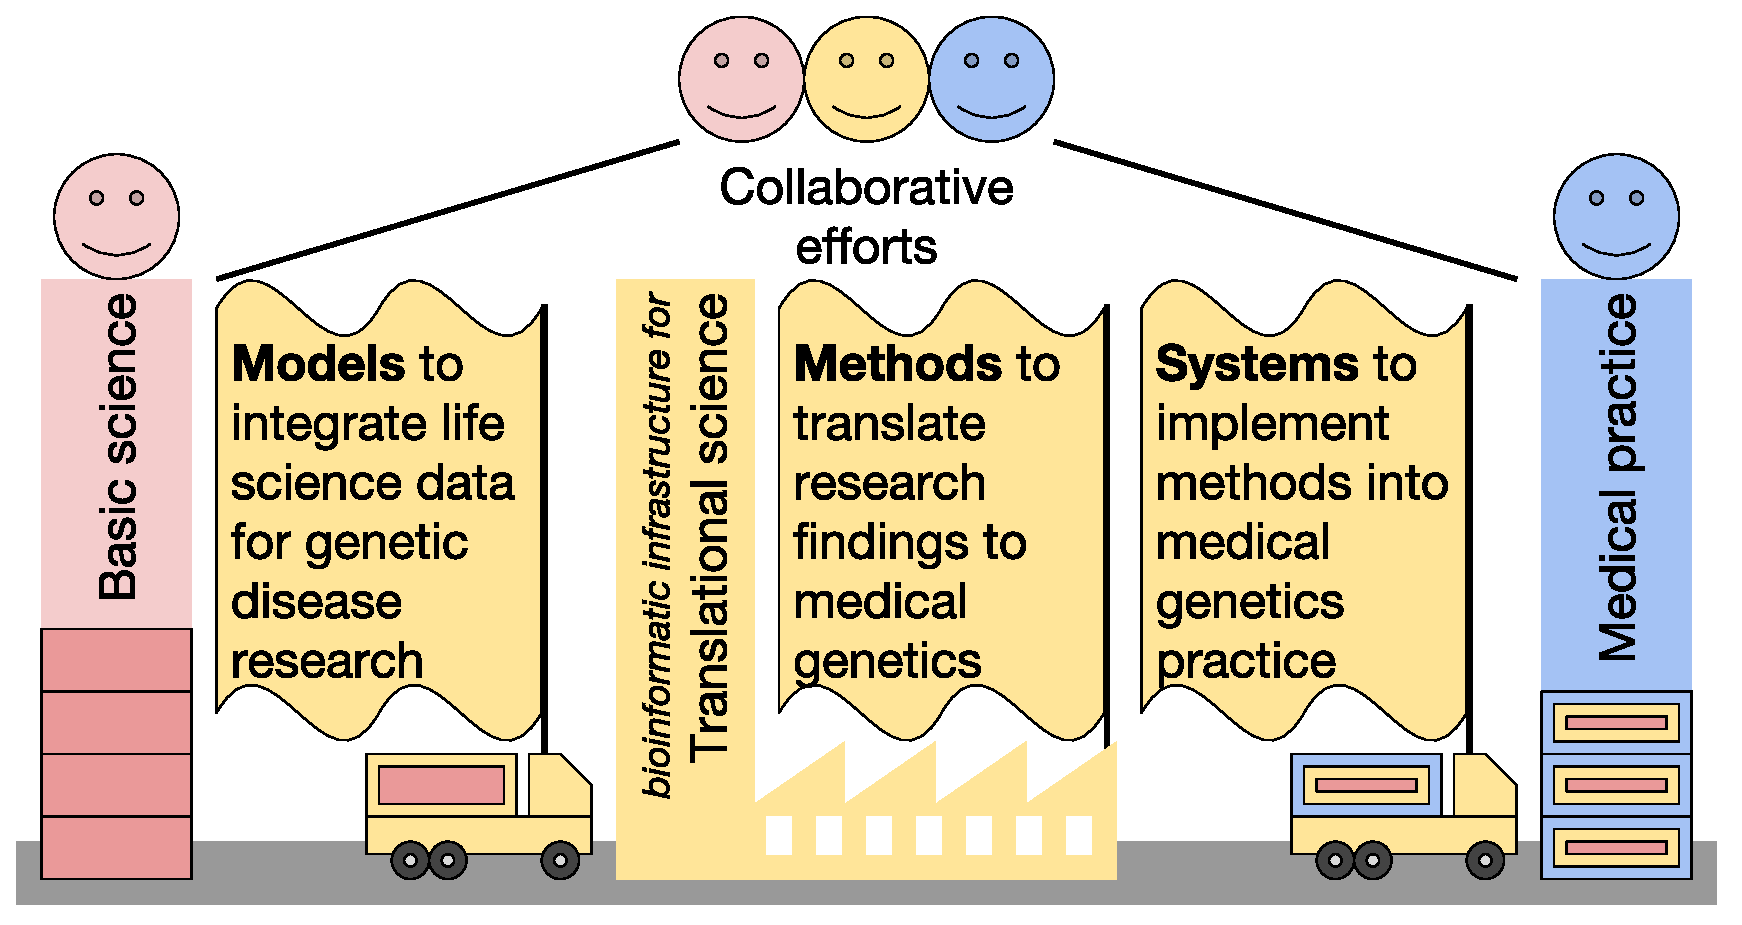
\includegraphics[width=1.0\linewidth]{img/introduction_overview}
\caption[Translational science overview]{Overview of bioinformatic infrastructure for translational science. Fundamental knowledge originates in basic research (red). Translational research (yellow) bridges the gap between basic research and medical practice (blue) by collaborative efforts from all parties involved.}
\label{fig:introduction_overview}
\end{figure}

Reference genomes - Population studies can tell us what to expect in the average individual.
Through phenotypic and molecular characterization of large groups of healthy individuals, we can establish a reference population.
Strong deviation from this reference may point towards causal mechanisms of molecular disease for more severe disorders that are highly damaging or otherwise debilitating at a younger age.

Association studies - Patient studies can tell us how disorders originate.
While studying small numbers of individuals can still uncover new Mendelian disease genes\cite{Witteveen_2016}, larger number of patients are required for statistical association of new disease candidate genes with less obvious effects\cite{Lelieveld_2016}.
By using extremely large sample sizes, we can also detect genetic associations for complex but more common afflictions such as celiac disease or obesity.

Additional molecular data - The genome is the prime information carrier within a living cell, but many more molecular levels stand between the DNA sequence and the eventual expression of a phenotype.
By measuring these different levels we can attempt to reconstruct both the lateral interactions (protein-protein interactions or gene co-expression networks) and perpendicular interactions (protein binding to the genome to silence expression or metabolite accumulation causing neurodegeneration), which can help to understand the workings of disease in detail.

Computational and 'big data' approaches - The rich collection of current life science data provides great opportunities for the development of smart software programs, computational algorithms and statistical tools that can extract knowledge from these growing data resources.
These must perform a multitude of roles and functions, including cleaning and quality control of raw data, imputing missing data points, finding statistical associations, modeling and running predictors, or constructing and pruning networks of detected relations.
In the following paragraphs I will explore these opportunities in detail.

\subsection{Population reference genomes}
Genomes are relatively similar between individuals, therefore, instead of assembling the complete sequence for each person, we only determine points of DNA variation compared to a reference genome.
Subsequently, we can aggregate the results by counting how often each point of variation was observed.
This allows us to store the information of thousands of genomes in files that are still quite computationally manageable and require smaller amounts of data storage capacity.
There are a number of initiatives that have collected the DNA variation of healthy individuals, such as the Thousand Genomes project\cite{McVean_2012} (2,504 genomes), the Genome of the Netherlands\cite{Francioli_2014} (750 genomes), the Exome Aggregation Consortium\cite{Lek_2016} (60,706 exomes), the NHLBI Exome Sequencing Project\cite{EVS} (6,503 exomes) and the upcoming gnomAD from the ExAC authors\cite{Lek_2016} (126,216 exomes and 15,137 genomes).
Here, the term “healthy” refers to individuals who do not suffer from a severe inborn disorder.
They may still develop common late-onset diseases with genetic components such as type 2 diabetes, cardiovascular problems, obesity or common forms of cancer.

These large reference sets find eager uptake in all areas of genetics including research and genome diagnostics.
Variants observed to have a high allele frequency in a population of individuals are called polymorphisms.
Such polymorphisms are very unlikely to directly cause a disease, although they might still act as modifiers (or markers) for disease risk\cite{Donald_2017}.
We may apply a filter based on Minor Allele Frequency (MAF): the alternative allele fraction compared to the most frequent reference allele.
A typical setting may be to exclude any variant from further analysis of a patient's genome when it occurs more than 1\% in the general population.
Depending on the rarity and severity of a disease, we may want to use thresholds as low as 0.01\% (see chapter \ref{chap:gavin}) and as high as 5\%\cite{Strom_2011}.
We can also use the genotype zygocity counts, which is the number of individuals heterozygous or homozygous for an allele.
If only heterozygous genotypes are observed in the general healthy population, we may be dealing with a recessive-acting disease variant, which quickly becomes a candidate for being pathogenic when detected homozygously in a patient.

As other types of population reference data becomes available, e.g. from RNA-sequencing\cite{Deelen_2015}, we have the opportunity to also establish a baseline for healthy individuals for data other than DNA variation.
We can use these references to investigate and manually predict potential pathogenic effects in patients and capture the outcomes.
These results are then used to develop tools to speed up the interpretation of new patient data and initiate a synergistic process leading to exponential tool development.

Furthermore, big population data provide insight into our genomic architecture.
The mention of Mendelian disease genes may give the impression that our genomes are fragile, but there is also evidence that shows they are surprising resilient.
Each healthy human has about 100 Loss of Function (LoF) variants with ~20 genes completely in\-ac\-ti\-va\-ted\cite{MacArthur_2012}.
We now have enough reference data to calculate an accurate LoF rate for every gene\cite{Lek_2016}, and this rate may be compared to a null distribution to determine which genes are LoF-tolerant and which are not. 
Any LoF-intolerant genes found in patients with severe mutations can then be prioritized as potentially disease-causing.
By analyzing the selection pressure on truncating variants we can then characterize genes, and estimate whether one or two dysfunctional alleles are likely to be disease causative\cite{Cassa_2017}.

Lastly, these large reference sets have put things in new perspective.
Some variants that were previously thought to be surely disease-causing were found to have low \textsl{penetrance}, meaning that not every individual with that mutation actually becomes ill\cite{Minikel_2016}.
Other variants once thought to have pathogenic effects have turned out to be far too common with respect to disease prevalence, revealing them as false positives\cite{Walsh_2016}.
Finally, on a more critical note, ethnicity biases in these reference sets may result in misclassifications\cite{Manrai_2016}, indicating a need for more diverse and representative data sets to be used in genome diagnostic interpretation.

\subsection{Genomic association studies}
In Mendelian or \textsl{monogenic} genetic disorders, a single dysfunctional gene can cause severe problems.
There are, however, numerous disease-related phenotypes that are not attributable to just one or a few genes.
Instead, many locations (or \textsl{loci}) on the genome seem to each contribute a small amount to the risk of the disease\cite{McCarthy_2008,Manolio_2009,Boyle_2017}.
Finding these weak associations requires large Genome-Wide Association Studies or \textsl{GWAS} which may include more than 250,000 participants\cite{Wood_2014}.
These large samples sizes can be achieved by genotyping arrays which can cheaply ascertain alleles of a predetermined set of variants.

In human, we have currently discovered about 30,000 trait-genome associations\cite{Welter_2013}.
While these include general traits like word reading ability, alcohol consumption, hair color, height, and freckling, most traits are of medical relevance and include susceptibility to common diseases such as hypertension, arthritis, celiac disease, cancer subtypes, diabetes, cardiovascular disease, ulcerative colitis, obesity, allergies, psoriasis and asthma.

Establishing these associations is important for several reasons.
Most notably, the locations where they are found implicate nearby genes that may be involved, making these genes the best candidates for further study.
However, genes must be carefully considered because the closest gene is often not relevant and statistical approaches have been developed\cite{Zhu_2016} to identify the strongest candidate in the region.

Another application of GWAS associations is modeling of genetic risk scores.
The effect size of the risk-associated alleles that an individual is harboring can be summed to a genetic risk score\cite{Dudbridge_2013}.
This risk, by definition, correlates to either the chance of developing a certain disease or the occurrence of a clinical event\cite{Malik_2014}, but genetic risk scores can also predict the quantitative severity of a clinical phenotype\cite{Belsky_2013}.

Based on a higher risk score, individuals may choose to undergo a specific medical check regularly, or adjust their lifestyles to improve their odds of not developing a certain disease.
Conversely, individuals with strong protective alleles might need fewer periodic examinations than usual, allowing physicians to spend more time on people with a higher risk.

\subsection{Additional molecular data}

Beyond the DNA sequence, much additional molecular data can now be gathered that can be used to identify which DNA variations are relevant for health and disease, and which are not.
Regulation of gene transcription, translation, protein activity and degradation constantly takes place at between different molecular levels.
For instance, the genes on the genome itself can be made harder to transcribe through methylation of the cytosine and adenine nucleotides\cite{Bird_2002}.
In addition, the chromosomal structure of DNA can be decondensated by histone acetylation (transfer of acetyl groups to DNA organizational elements), making it more accessible for transcription\cite{Eberharter_2002}.
The transcriptional expression of genes is further regulated by genetic variants themselves\cite{Albert_2015}.
Finally, proteins form a complex network of interactions\cite{Phizicky_1995} that, in turn, also regulate gene expression\cite{Taniguchi_2012}.

We study the complex patterns of this regulation to understand how genes act in concert, and how a disease phenotype presents in cells, tissues and organisms.
Large initiatives that pursue this goal include studies into expression quantitative trait loci (eQTL)\cite{Westra_2013} and allele-specific expression\cite{Deelen_2015}, characterization of functional genomic elements including methylation and acetylation patterns\cite{Dunham_2012}, comprehensive expression studies across different tissues\cite{Lonsdale_2013} and cell types\cite{Forrest_2014}.

These same kinds of studies can also be performed on model organisms, which can be bred and measured in highly controlled environments for pin-point phenotypic and molecular characterization.
Studies on mice have been an essential tool for biological research for more than a century and continue their important role today\cite{Phifer_Rixey_2015}.
Mice are evolutionarily relatively close to humans, and their size and short generation time allows experiments to be set up and run with large enough numbers for statistical significance.
However, other types of model organisms such as zebrafish\cite{Lieschke_2007} and worm\cite{Kaletta_2006} can offer unique advantages over using rodents.
While these organisms have a larger evolutionary distance to humans, they are cheaper, faster and easier to breed and have transparent bodies that are easy to dissect.
The tiny \textsl{C. elegans} worm has by far the fastest life cycle, simplest anatomy and the unique property of strains that can be frozen and revived.

In addition to transcriptomics and epigenetics, we can also measure the levels of metabolites and proteins present in cells.
These technologies, known as metabolomics and proteomics, can be integrated with genomics data\cite{Grapov_2015} to obtain a more complete understanding of the complex processes in the cell that interplay with all these layers.
Finally, we can also investigate the genomic variation that prevents disease or even increase our health instead of looking for genes that make people ill.
The search for so-called 'protective alleles' is an up and coming area of study that will also result in healthcare advancements\cite{Harper_2015}.

\subsection{Computational and 'big data' approaches}

Measuring and interpreting the large, complex and diverse life-science datasets has driven the development of a plethora of new computational methods and tools to analyze these data.
These include methods to clean and prepare data for analysis, advanced statistical methods, relational databases, web applications, data integration and visualization tools.

A few notable examples include the Variant Quality Score Recalibration (VQSR), a module of the Genome Analysis Toolkit (GATK)\cite{Van_der_Auwera_2013}.
This tool performs comparative machine learning on identified (\textsl{called}) NGS variants versus a reference truth set to find the optimal variables for determining which variants are true positives and which are false.

Variants can also be determined using genotyping platforms, but when multiple platforms are used, data are not comparable.
However, they can be harmonized by inferring missing variants using genotype imputation\cite{Deelen_2014}, which also uses reference knowledge.

After variants are determined, there are many tools that estimate variant pathogenicity to assist genome diagnostics or research into genetic diseases\cite{Eilbeck_2017}.
A powerful method to prioritize variants for further interpretation are CADD scores\cite{Kircher_2014}.
These scores are a measure of evolutionary pressure on genetic variants that builds upon 60+ existing tools and sources.
Variants with a higher score are more likely to be deleterious and are therefore the best candidates in disease research.

Using CADD scores, variants are discovered in genes of which the function is not yet known.
Knowledge net\-works such as Gene\-MA\-NIA\cite{Warde_Farley_2010} may help to infer a putative function by linking unknown genes to genes known from previous studies to show a similar expression pattern.
We can also characterize unknown genes by their evolutionary, loss-of-function and network interaction properties to prioritize candidate variants\cite{Khurana_2013} and even predict disease inheritance mode to a certain degree\cite{Hsu_2016}.

Taking this approach a step further, GeneNetwork\cite{Fehrmann_2015} is constructed from co-regulation patterns found within tens of thousands of samples for which gene expression was measured.
GeneNetwork provides unprecedented resolution and predictive power across multiple cell types and tissues.
Analogous to discovering patterns in expression data, the network of protein-protein interactions can also be computationally predicted using various methods\cite{Zahiri_2013}.

The combined current knowledge of how cells control functions such as growth, movement, differentiation, metabolism, communication, and response to stress or pathogens is captured in high-level pathway databases such as WikiPathways\cite{Kutmon_2015}, Reactome\cite{Fabregat_2015} or KEGG\cite{Kanehisa_2015}.

Taken together, these tools provide important clues for wet-lab studies, which then in turn provide better and more meaningful biological measurements that can help to develop new and improved methods.


\section{Thesis outline} \label{intro_outline}

In this thesis I show how, by addressing data challenges and bioinformatics opportunities in translational infrastructure, we can advance our genetic knowledge and its application in medical genetics.
The focus of the first two chapters is on models that integrate life science data as a basis for finding new gene-disease associations.
I then develop methods to discover leads for human disease and utilize pathogenicity estimates for clinical application. 
Finally, I implement software systems that translate what we have learned to medical genetics practice.
An overview of the chapter progression in this thesis is shown in Figure \ref{fig:introduction_chapters}.

\begin{figure}
\centering
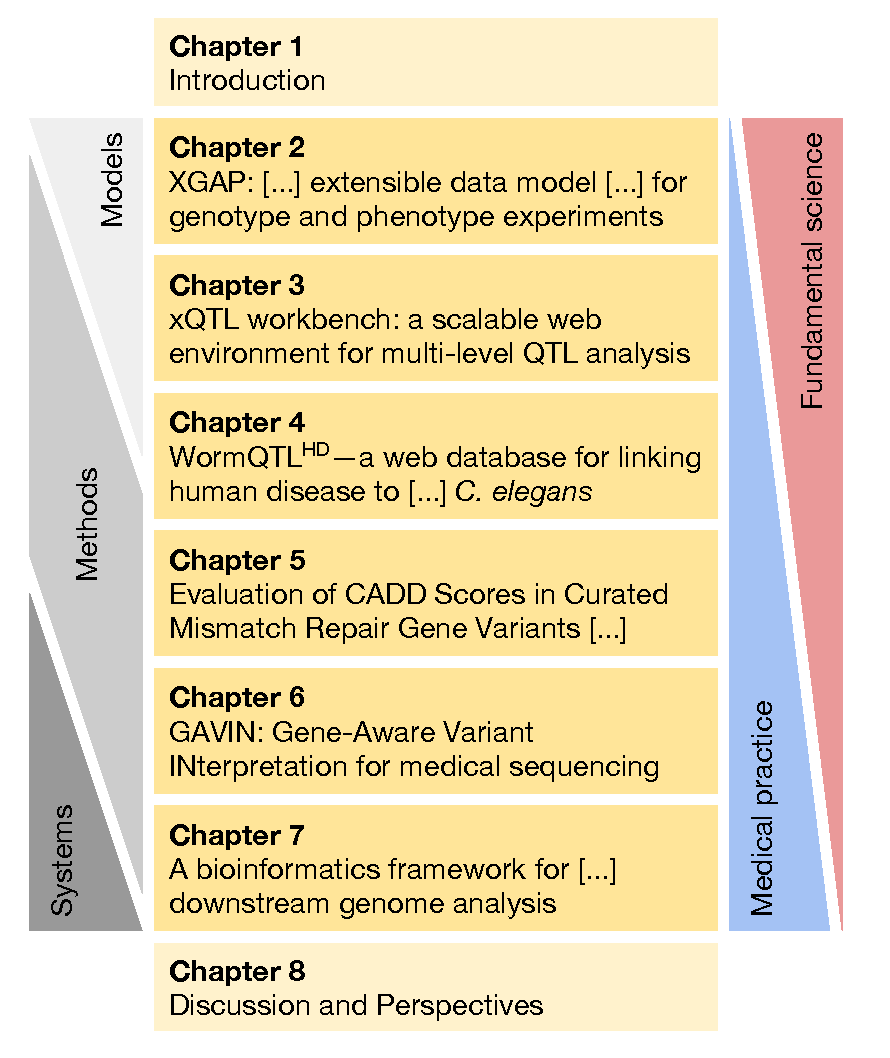
\includegraphics[width=1.0\linewidth]{img/introduction_chapters.eps}
\caption[Overview of thesis chapter progression]{Overview of thesis chapter progression in terms of type of output and area of application. We can define an overall gradient from fundamental science to medical practice, as well as transitions from models to integrate life science data towards methods to translate discovered knowledge and systems to implement new methods into patient care.}
\label{fig:introduction_chapters}
\end{figure}

\subsection[New models to integrate life science data]{New models to integrate life science data for genetic disease research (chapters \ref{chap:xgap} and \ref{chap:xqtl})}

There are many approaches for gathering, structuring, integrating and analyzing life science data, each best suited to test a spe\-ci\-fic hy\-po\-the\-sis\cite{Ritchie_2015}.
To help domain experts test new ideas and quickly interpret interesting findings, they should be able run the necessary queries, tools and visualizations themselves.
To achieve this, the underlying data has to be both properly modeled ('computer-readable') and fortified with enough metadata to describe what the data means\cite{Wilkinson_2016} so that it can be automatically addressed by applicable tools.

As data volumes grow ever larger, these tools have to be executed on external high-throughput computational environments such as multi-node computer clusters.
To facilitate storage of these huge datasets and parallelized computation, we investigated how to store complex data using the flexible XGAP model in chapter \ref{chap:xgap}, and used this as a basis to develop xQTL workbench in chapter \ref{chap:xqtl}.
xQTL workbench is a flexible database system designed to store any genotype and phenotype information with basic visualization and computational capabilities.

\subsection[New methods to translate research findings]{New methods to translate research findings to medical genetics (chapters \ref{chap:wormqtl} and \ref{chap:caddmmr})}

Translational medicine investigates how relevant new findings can be used to improve patient diagnosis and care.
To demonstrate how new findings can be generated, we loaded almost 100 data sets of \textsl{C. elegans} into an xQTL database, containing around 300 million measurements.
To show value for human health applications, we connected worm phenotypes to human disease at a molecular level using protein orthology.
Chapter \ref{chap:wormqtl} shows how these data can now be used to find models and leads for human disease research.
Furthermore, a biologist-friendly online environment enables the research community to join in and dig through the data.

Interesting findings need to be explored further and placed into clinical context before medical genetics can benefit from them.
The previously mentioned CADD scores\cite{Kircher_2014} are an example of an innovation with great potential.
Doctors and clinical geneticists have an interest in such developments, but cannot use it in practice without guidelines about how to interpret these scores in patient cases.
To explore how such a guideline is created and used, we translated CADD scores to the clinical classification of variants in mismatch repair genes in chapter \ref{chap:caddmmr}.
These genes may harbor variants that cause hereditary colorectal cancer.
By characterizing these scores in this context, we learned both their pitfalls and how they can be used to prioritize new mutations or double-check existing classifications.

\subsection[New systems for medical genetics practice]{New systems to implement methods into medical genetics practice (chapters \ref{chap:gavin} and \ref{chap:frameworkforgenomics})}

Large reference datasets and computational resources, when guided by translational research, should allow us to transform patient care.
To facilitate this, we need to design, build and maintain reliable software systems\cite{Prins_2015} running on a stable server and database infrastructure\cite{Swertz_2007}.
These systems must handle rapidly increasing quantities of whole-ge\-no\-me data as sequencing costs dropped from a billion dollars to just a thousand dollars per patient.
The data produced needs to be contrasted against large population reference sets and other patient genomes for research, interpretation or diagnosis using computational methods.
The storage, processing and filtering solutions for these massive datasets need the capabilities to be scaled up, fine-tuned and clinically validated accordingly.

Encouraged by results of chapter \ref{chap:caddmmr}, we generalized the CADD score calibration approach and applied it to $>$3,000 disease genes.
We emphasize practical use by excluding variants that would also excluded by existing methods.
On the variants that remain that are hard to interpret, we find out if CADD scores can be of further help.
The resulting predictor tool, GAVIN, is described in chapter \ref{chap:gavin} and works remarkably well for clinically characterized genes.
It serves as a first-lead causal variant screening tool with broad application in clinical genomics.

This work then feeds into chapter \ref{chap:frameworkforgenomics}, where we define a framework to automate the interpretation of genomic data, and to fast-track innovations in this process. 
We implement the GAVIN+ interpretation tool, which combines GAVIN with additional knowledge and criteria from clinical genetics to quickly identify variants and genotypes that are potentially disease-causing.
This tool outputs its result in the new rVCF (Report VCF) format, which captures any relevant analysis results along with detailed provenance information and the reason why a variant is of interest.

Using this format, we can run fast validation on known pathogenic variants and estimation of false discovery rate on healthy control samples.
The final result can be visualized in a customizable doctor-friendly report, analyzed further as the format is fully compliant with existing tools, and shared with peers.
The modular framework design separates the enrichment, interpretation and visualization of the data.

Our proposed solution is flexible and maintainable and its standardized formats allows the community to develop focused software tools that produce and utilize these files.
As a result, newly developed methods can be quickly adapted and validated within local installation of the framework.
This high-throughput infrastructure will speed up molecular diagnostic practice, and prepare it for seamless future integration of new analysis methods and powerful new omics techniques.

\chapter[XGAP model for genotype and phenotype experiments]{XGAP: A uniform and extensible data model and software platform for genotype and phenotype experiments}
\chaptermark{XGAP model for genotype and phenotype}
\label{chap:xgap}

{ \Large \leftwatermark{
\put(-67,-66.5){ 1 }
\put(-76.5,-100){\includegraphics[scale=0.8]{img/thumbindex.eps}} \put(-67,-91.5){ {\color{white} 2 }}
\put(-67,-116.5){ 3 }
\put(-67,-141.5){ 4 }
\put(-67,-166.5){ 5 }
\put(-67,-191.5){ 6 }
\put(-67,-216.5){ 7 }
\put(-67,-241.5){ 8 }
} \rightwatermark{
\put(350.5,-66.5){ 1 }
\put(346.5,-100){\includegraphics[scale=0.8]{img/thumbindex.eps}} \put(350.5,-91.5){ {\color{white} 2 }}
\put(350.5,-116.5){ 3 }
\put(350.5,-141.5){ 4 }
\put(350.5,-166.5){ 5 }
\put(350.5,-191.5){ 6 }
\put(350.5,-216.5){ 7 }
\put(350.5,-241.5){ 8 }
}}

\hfill \underline{Genome Biol.} 2010;11(3):R27.

\hfill DOI: \href{https://doi.org/10.1186/gb-2010-11-3-r27}{10.1186/gb-2010-11-3-r27}

\hfill PubMed ID: \href{https://www.ncbi.nlm.nih.gov/pubmed/20214801}{20214801}

\newpage

\noindent
Morris A. Swertz\textsuperscript{1,2,3,*}, K. Joeri van der Velde\textsuperscript{1,2}, Bruno M. Tesson\textsuperscript{2}, Richard A Scheltema\textsuperscript{2}, Danny Arends\textsuperscript{1,2}, Gonzalo Vera\textsuperscript{2}, Rudi Alberts\textsuperscript{4}, Martijn Dijkstra\textsuperscript{5}, Paul Schofield\textsuperscript{6}, Klaus Schughart\textsuperscript{4}, John M. Hancock\textsuperscript{7}, Damian Smedley\textsuperscript{3}, Katy Wolstencroft\textsuperscript{8}, Carole Goble\textsuperscript{8}, Engbert O. de Brock\textsuperscript{9}, Andrew R. Jones\textsuperscript{10}, Helen E. Parkinson\textsuperscript{3}, members of the Coordination of Mouse Informatics Resources (CASIMIR)\textsuperscript{6}, Genotype-To-Phenotype (GEN2PHEN) Consortiums\textsuperscript{1}, Ritsert C. Jansen\textsuperscript{1,2}\\

\noindent
1. Genomics Coordination Center, Department of Genetics, University Medical Center Groningen and University of Groningen, 9700 RB Groningen, The Netherlands\\
2. Groningen Bioinformatics Center, University of Groningen, 9750 AA Haren, The Netherlands\\
3. EMBL - European Bioinformatics Institute, Hinxton, Wellcome Trust Genome Campus Hinxton, Cambridge CB10 1SD, UK\\
4. Experimental Mouse Genetics, Helmholtz Center for Infection Research, Inhoffenstraße 7, D-38124 Braunschweig, Germany\\
5. Center for Medical Biomics, University of Groningen, Groningen, A. Deusinglaan 1, 9713 AV Groningen, The Netherlands\\
6. Physiological Development and Neuroscience, University of Cambridge, Downing Street, Cambridge CB2 3DY, UK
7. Bioinformatics Group, MRC Harwell, Harwell, Oxfordshire OX11 0RD, UK\\
8. Information Management Group, School of Computer Science, University of Manchester, Kilburn Building, Oxford Road, Manchester M13 9PL, UK\\
9. Department of Business and ICT, Faculty of Economics and Business, University of Groningen, 9700 AV Groningen, The Netherlands\\
10. Department of Pre-Clinical Veterinary Science and Veterinary Pathology, Faculty of Veterinary Science, University of Liverpool, Liverpool L69 7ZJ, UK\\

\noindent
Received 2009 Jul 14; Revised 2009 Dec 17; Accepted 2010 Mar 9.
\\~\\
* Corresponding author.


\section*{Abstract}
We present an extensible software model for the genotype and phenotype community, XGAP.
Readers can download a standard XGAP (\url{http://www.xgap.org}) or auto-generate a custom version using MOLGENIS with programming interfaces to R-software and web-services or user interfaces for biologists.
XGAP has simple load formats for any type of genotype, epigenotype, transcript, protein, metabolite or other phenotype data.
Current functionality includes tools ranging from eQTL analysis in mouse to genome-wide association studies in humans.

\section{Background}
Modern genetic and genomic technologies provide researchers with unprecedented amounts of raw and processed data.
For example, recent genetical genomics\cite{Li_2008, Jansen_2001, Li_2005} studies have mapped gene expression (eQTL), protein abundance (pQTL) and metabolite abundance (mQTL) to genetic variation using genome-wide linkage and genome-wide association experiments on various microarray, mass spectrometry and proton nuclear magnetic resonance (NMR) platforms and in a wide range of organisms, including human\cite{Editorial_2007, G_ring_2007, Dixon_2007, Stranger_2007a, Heap_2009}, yeast\cite{Brem_2002, Foss_2007}, mouse\cite{Bystrykh_2005}, rat\cite{Hubner_2005}, \textsl{Caenorhabditis elegans}\cite{Li_2006} and \textsl{Arabidopsis thaliana}\cite{Keurentjes_2007, Keurentjes_2006, Fu_2009}.

Understanding these and other high-tech genotype-to-phenotype data is challenging and depends on suitable ‘cyber infrastructure’ to integrate and analyze data\cite{Stein_2008, Fay_2008}: data infrastructures to store and query the data from different organisms, biomolecular profiling technologies, analysis protocols and experimental designs; graphical user interfaces (GUIs) to submit, trace and retrieve these particular data; communicating infrastructure in, for example, R\cite{Ihaka_1996}, Java and web services to connect to different processing infrastructures for statistical analysis\cite{Carey_2006, Alberts_2007, Fu_2007, Bhave_2007, Broman_2003} and/or integration of background information from public databases\cite{Smedley_2008}; and a simple file format to load and exchange data within and between projects.

Many elements of the required cyber infrastructure are available: The Generic Model Organism Database (GMOD) community developed the Chado schema for sequence, expression and phenotype data\cite{Mungall_2007} and delivered reusable software components like gbrowse\cite{Stein_2002}; the BioConductor community has produced many analysis packages that include data structures for particular profiling technologies and experimental protocols\cite{Gentleman_2004}; and numerous bespoke databases, data models, schemas and formats have been produced, such as the public and private microarray expression databases and exchange formats\cite{Brazma_2006, Saal_2002, Galperin_2009}.
Some integrated cyber infrastructures are also available: the National Center for Biotechnology Information (NCBI) has launched dbGaP (database of genotypes and phenotypes)\cite{Mailman_2007}, a public database to archive genotype and clinical phenotype data from human studies; and the Complex Trait Consortium has launched GeneNetwork\cite{Chesler_2005}, a database for mouse genotype, classical phenotype and gene expression phenotype data with tools for ‘per-trait’ quantitative trait loci (QTL) analysis.

However, a suitable and customizable integration of these elements to support high throughput genotype-to-phenotype experiments is still needed\cite{Thorisson_2009b}: dbGaP, GeneNetwork and the model organism databases are designed as international repositories and not to serve as general data infrastructure for individual projects; many of the existing bespoke data models are too complicated and specialized, hard to integrate between profiling technologies, or lack software support to easily connect to new analysis tools; and customization of the existing infrastructures dbGaP, GeneNetwork or other international repositories\cite{Zeng_2007, Hu_2007} or assembly of Bioconductor and generic model organism database components to suit particular experimental designs, organisms and biotechnologies still requires many minor and sometimes major manual changes in the software code that go beyond what individual lab bioinformaticians can or should do, and result in duplicated efforts between labs if attempted.

To fill this gap we here report development of an extensible data infrastructure for genotype and phenotype experiments (XGAP) that is designed as a platform to exchange data and tools and to be easily customized into variants to suit local experimental models.
We therefore adopted an alternative software engineering strategy, as outlined in our recent review\cite{Swertz_2007}, that enables generation of such software efficiently using three components: a compact and extensible ‘standard’ model of data and software; a high-level domain-specific language (DSL) to simply describe biology-specific customizations to this software; and a software code generator to automatically translate models and extensions into all low-level program files of the complete working software, building on reusable elements such as listed above as well as general informatics elements and some new/optimized elements that were missing.

Below we detail XGAPs extensible ‘standard’ software model (XGAP-OM) and evaluate the auto-generated text file exchange format (XGAP-TAB) and customizable database software (XGAP-DB) that should help researchers to quickly use and adapt XGAP as a platform for their genetics and/or *omics experiments (Table \ref{table:xgap_features}).
Harmonized data representations and programmatic interfaces aim to reduce the need for multiple format convertors and easy sharing of downstream analysis tools via a hub-and-spoke architecture.
Use of software auto-generation, implemented using MOLGENIS, aims to ease and speed up customization/variation into new XGAP versions for new biotechnologies and alternative experimental designs while ensuring consistent programming interfaces for the integration and sharing of existing analysis tools.
Standardized extension mechanisms should balance between format/interface stability for existing data types and tools, and flexibility to adopt new ones.

\begin{table}
\footnotesize
\begin{tabularx}{\linewidth}{ l X }
  \hline
  \rule{0pt}{2.5ex}\textbf{Store} & Store genotype and phenotype experimental data using only four ‘core’ data types: \textsl{Trait}, \textsl{Subject}, \textsl{Data}, and \textsl{DataElement}. For example: a single-channel microarray reports raw gene expression \textsl{Data} for each microarray probe \textsl{Trait} and each individual \textsl{Subject}. Add information on data provenance by giving details in \textsl{Investigation}, \textsl{Protocols} and \textsl{ProtocolApplications}\\
  \rule{0pt}{2.5ex}\textbf{Customize} & Customize ‘my’ XGAP database with extended variants of \textsl{Trait} and \textsl{Subject}. In the online XGAP demonstrator, \textsl{Probe} traits have a sequence and genome location and \textsl{Strain} subjects have parent strains and (in)breeding method. Describe extensions using MOLGENIS language and the generator automatically changes XGAP database software to your research\\
  \rule{0pt}{2.5ex}\textbf{Upload} & Upload data from measurement devices, public databases, collaborating XGAP databases, or a public XGAP repository with community data. Simply download trait information as tab-delimited files from one XGAP and upload it into another; this works because of the uniformity of the core data types (and extensions thereof)\\
  \rule{0pt}{2.5ex}\textbf{Search} & Search genetical genomics data using the graphical user interface with advanced query tools. The uniformity of the ‘code generated’ interfaces make it easy to learn and use interfaces for both ‘core’ data types as well as customized extensions\\
  \rule{0pt}{2.5ex}\textbf{Analyze} & Analyze data by connecting tools using simple methods in Java, R, Web Services or Internet hyperlinks. For example, map and plot quantitative trait loci in R using XGAP data retrieved via the R interface\\
  \rule{0pt}{2.5ex}\textbf{Plug-in} & Plug-in the best analysis tools into the user interface so biologists can use them. Bioinformaticians are provided with simple mechanisms to seamlessly add such tools to XGAP, building on the automatically generated GUI and API building blocks\\
  \rule{0pt}{2.5ex}\textbf{Share} & Share data, customizations, connected analysis tools and user interface plug-ins with the genetical genomics community, using XGAP as exchange platform. For example, the MetaNetwork R package can talk to data in XGAP. This makes it easy for other XGAP owners to also use it\\
  \hline
  ~ & {\scriptsize API: application programming interface; GUI: graphical user interface; MOLGENIS: biosoftware generator for MOLecular GENetics Information Systems.}\\
\end{tabularx}
\caption[Features of XGAP database]{Features of XGAP database for genotype and phenotype experiments.}
\label{table:xgap_features}
\end{table}

\section{Minimal and extensible object model}
We developed the XGAP object model to uniformly capture the wide variety of (future) genotype and phenotype data, building on generic standard model FuGE (Functional Genomics Experiment)\cite{Jones_2007} for describing the experimental ‘metadata’ on samples, protocols and experimental variables of functional genomics experiments, the OBO model (of the Open Biological and Biomedical Ontologies foundry for use of standard and controlled vocabularies and ontologies that ease integration\cite{Smith_2007}, and lessons learned from previous, profiling technology-specific modeling efforts\cite{Brazma_2006}.

Figure \ref{fig:xgap_model}b shows the core components of a genotype-to-phenotype investigation: the biological subjects studied (for example, human individuals, mouse strains, plant tissue samples), the biomolecular protocols used (for example, Affymetrix, Illumina, Qiagen, liquid chromatography-mass spectrometry (LC/MS), Orbitrap, NMR), the trait data generated (usually data matrices with, for example, phenotype or transcript abundance data), the additional information on these traits (for example, genome location of a transcript, masses of LC/MS peaks), the wet-lab or computational protocols used (for example, MetaNetwork\cite{Fu_2007} in the case of QTL and network analysis) and the derived data (for example, QTL likelihood curves).

\linespread{1.00} % need to squeeze a bit to fit caption nicely
\begin{figure}
	\centering
	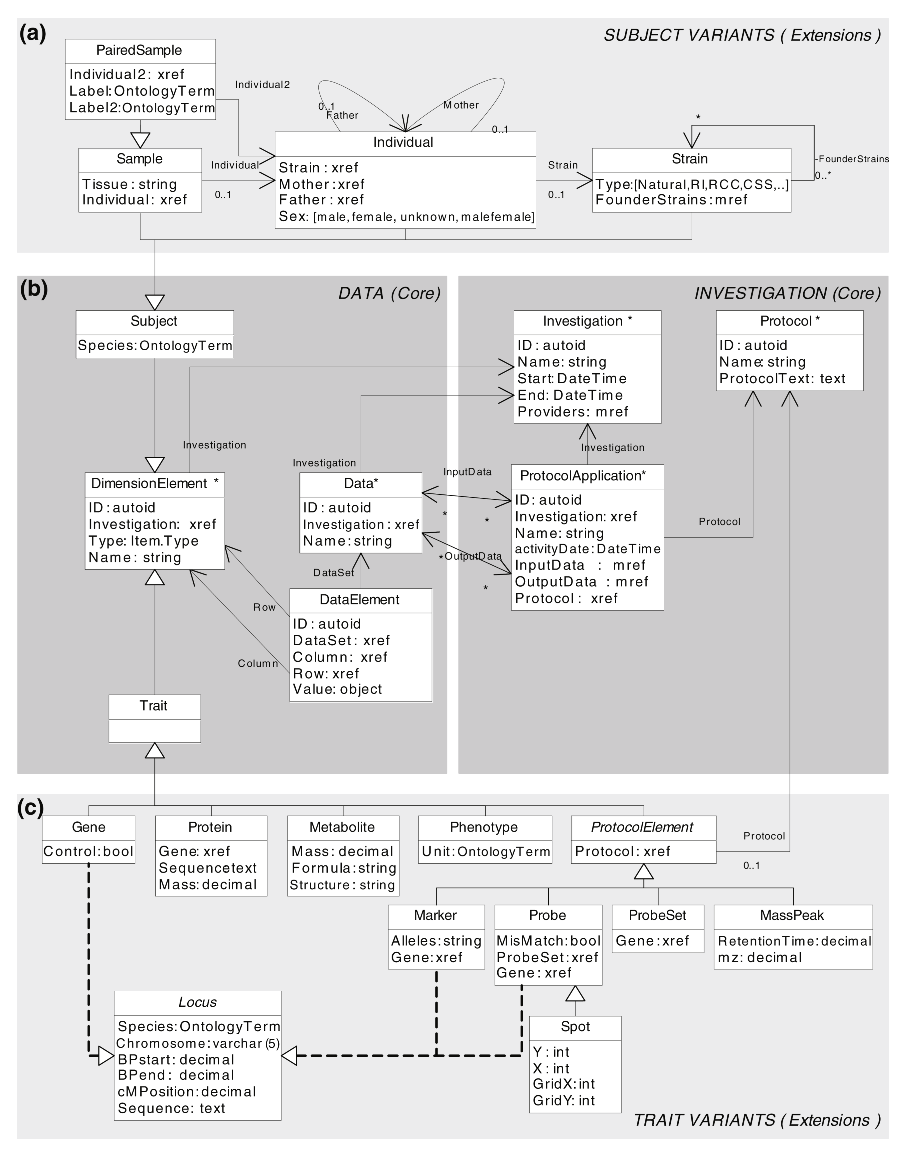
\includegraphics[width=0.87\linewidth]{img/xgap_model}
	\captionsetup{font=scriptsize,labelfont=scriptsize}
	\caption[Extensible genotype and phenotype object model]{Extensible genotype and phenotype object model. Experimental genotype and (molecular) phenotype data can be described using \textsl{Subject}, \textsl{Trait}, \textsl{Data} and \textsl{DataElement}; the experimental procedures can be described using \textsl{Investigation}, \textsl{Protocol} and \textsl{ProtocolApplication} \textbf{(b)}. Specific attributes and relationships can be added by extending core data types, for example, \textsl{Sample} and \textsl{Gene} \textbf{(a, c)}. See Table \ref{table:xgap_core_usecases}, \ref{table:xgap_extension_usecases} and \ref{table:xgap_annotation_usecases} for uses of this model. The model is visualized in the Unified Modeling Language (UML): arrows denote relationships (\textsl{Data} has a field Investigation that refers to \textsl{Investigation} ID); triangle terminated lines denote inheritance (\textsl{Metabolite} inherits all properties ID, Name, Type from \textsl{Trait}, next to its own attributes Mass, Formula and Structure); triangle terminated dotted lines denote use of interfaces (\textsl{Probe} ’implements’ properties of \textsl{Locus}); relationships are shown both as arrows and as properties (’xref’ for one-to-many, ‘mref’ for many-to-many relationships). Asterisks mark FuGE-derived types (for example, \textsl{Protocol}*).}
	\label{fig:xgap_model}
\end{figure}
\linespread{1.05} % and back to normal

We describe these biological components using FuGE data types and XGAP extensions thereof.
\textsl{Investigation} binds all details of an investigation.
Each investigation may apply a series of biomolecular\cite{Brown_2005} and computational\cite{Carey_2006, Alberts_2007, Fu_2007, Bhave_2007} \textsl{Protocols}.
The applications of such \textsl{Protocols} are termed \textsl{ProtocolApplications}, which in the case of computational \textsl{Protocols} may require input \textsl{Data} and will deliver output \textsl{Data}.
These \textsl{Data} have the form of matrices, the \textsl{DataElements} of which have a row and a column index.
Each row and column refers to a \textsl{DimensionElement}, being a particular \textsl{Subject} or a particular \textsl{Trait}.
Table \ref{table:xgap_core_usecases} illustrates the usage of these core data types.

\begin{table}
\begin{tabulary}{\linewidth}{L}
  \hline
  A growth measurement (\textsl{Data}) reports the time (\textsl{DataElement}) it took to flower (\textsl{Trait}) for an \textsl{Arabidopsis} plant (\textsl{Subject})\\
  ~\\
  A two-color microarray result (\textsl{Data}) describes raw intensities measured (\textsl{DataElement}) for gene transcript probe hybrdization (\textsl{Trait}) for each pair of \textsl{Arabidopsis} individuals (\textsl{Subject})\\
  ~\\
  A marker measurement (\textsl{ProtocolApplication}) resulted in a genetic profile (\textsl{Data}) with genotype values (\textsl{DataElement}) for each SNP/microsatellite marker (\textsl{Trait}) for each human individual (\textsl{Subject})\\
  ~\\
  A genetical genomics stem cell \textsl{Investigation} was carried out on 30 recombinant mouse inbred strains (\textsl{Subject}). It involved a \textsl{ProtocolApplication} of the ‘Affymetrix MG-U74Av2’ \textsl{Protocol} to produce expression profiles (\textsl{Data}) for 12,422*16 microarray probes (\textsl{Traits}). These profiles consisted of a matrix of signals (\textsl{DataElement}) for each Probe (\textsl{Traits}) and each InbredStrain (\textsl{Subject}). Subsequently, these \textsl{Data} were taken as \textsl{inputData} in a normalization procedure (\textsl{ProtocolApplication}) using RMA normalization \textsl{Protocol}, which resulted in \textsl{outputData} of normalized profiles (\textsl{Data}) of Probe*InbredStrain (Trait*Subject)\\
  \hline
  {\footnotesize RMA: robust multi-array average.}\\
\end{tabulary}
\caption{Use cases of core data types.}
\label{table:xgap_core_usecases}
\end{table}

Figure \ref{fig:xgap_model}a, c shows how the XGAP model can be extended to accommodate details on particular types of subjects and traits in a uniform way.
A \textsl{Trait} can be a classical phenotype (for example, flowering - the flowering time is stored in the \textsl{DataElement}) or a biomolecular phenotype (for example, \textsl{Gene} X - its transcript abundance is stored in the \textsl{DataElement}).
A \textsl{Trait} can also be a genotype (for example, \textsl{Marker} Y is a genomic feature observation that is stored in the \textsl{DataElement}).
Genomic traits such as \textsl{Gene}, \textsl{Marker} and \textsl{Probe} all need additional information about their genome \textsl{Locus} to be provided.
Similarly, a \textsl{Subject} can be a single \textsl{Sample} (for example, a labeled biomaterial as put on a microarray) and such a sample may originate from one particular \textsl{Individual}.
It may also be a \textsl{PairedSample} when biomaterials come from two individuals - for example, if biomaterial has been pooled as in two-color microarrays.
An individual belongs to a particular \textsl{Strain}.
When new experiments are added new variants of \textsl{Trait} and \textsl{Subject} can be added in a similar way.
Table \ref{table:xgap_extension_usecases} illustrates the generic usage of these extended data types.

\begin{table}
\begin{tabulary}{\linewidth}{L}
  \hline
  \textsl{Sample} is a \textsl{Subject} with the additional property that ‘Tissue’ can be specified\\
  ~\\
  \textsl{Individual} is a \textsl{Subject} with the additional property that relationships with Mother and Father individuals, as well as \textsl{Strain}, can be specified\\
  ~\\
  \textsl{PairedSample} is a \textsl{Sample} with the additional property that ‘Dye’ has to be specified and which two Subjects (or subclasses such as Individual) are labeled with ‘Cy3’ and ‘Cy5’\\
  ~\\
  An \textsl{InbredStrain} is a \textsl{Strain} with the additional property that the ‘Parents’ (mother Individual and father Individual) are specified and the ‘type’ of inbreeding used\\
  ~\\
  An amplified fragment length polymorphism, microsatellite or SNP \textsl{Marker} (is a \textsl{Trait}) may refer to genetic and possible genomics location (\textsl{Marker} also is a \textsl{Locus})\\
  ~\\
  A correlation computation (\textsl{Data}) reports associations (\textsl{DataElement}) between \textsl{Metabolite} (is a \textsl{Trait}); because \textsl{Trait} and \textsl{Subject} are both extensions of \textsl{DimensionElement}, they can be connected to a row and column of \textsl{DataElement} interchangeably\\
  \hline
\end{tabulary}
\caption[Use cases of extended data types]{Use cases of extended data types.}
\label{table:xgap_extension_usecases}
\end{table}

Several standard data types were also inherited from FuGE to enable researchers to provide ‘Minimum Information’ for QTLs and Association Studies such as defined in the MIQAS checklist\cite{xgap_miqas} - a member of the Minimum Information for Biological and Biomedical Investigations (MIBBI) guideline effort\cite{Taylor_2008}.
Data types \textsl{Action(Application)}, \textsl{Software(Application)}, \textsl{Equipment (Application)} and \textsl{Parameter(Value)} can be used to describe \textsl{Protocol(Application)s} in more detail.
For example, a normalization \textsl{Protocol} may involve a ‘robust multiarray average (RMA) normalization’ \textsl{Action} that uses Bioconductor ‘affy’ \textsl{Software}\cite{Irizarry_2003} with certain \textsl{ParameterValues}.
Data types \textsl{Description}, \textsl{BibliographicReferences}, \textsl{DatabaseEntry}, \textsl{URI}, and \textsl{FileAttachment} enable researchers to freely add additional annotations to certain data types - \textsl{DimensionElement}, \textsl{Investigation}, \textsl{Protocol}, \textsl{ProtocolApplication}, and \textsl{Data}.
For example, researchers can annotate a \textsl{Gene} with one or more \textsl{DatabaseEntries}, referring to unique database accession numbers for automated data integration.

A unique feature of XGAP is the uniform treatment of the various trait and subject annotations.
The drawback of allowing users to freely add additional annotations such as described above is that users and tools using metabolite and gene traits, for example, would have to inspect each \textsl{Trait} instance to see whether it is actually a metabolite or gene, and how it is annotated.
That is why we instead use the object-oriented method of ‘inheritance’ to explicitly add essential properties to \textsl{Trait} and \textsl{Subject} variants to make sure that they are described in a uniform way.
For example, \textsl{Metabolite} extends \textsl{Trait}, which explicitly adds properties ID, Name and Type (inherited from \textsl{DimensionElement}) to metabolite specific properties Mass, Formula and Structure.
See Jones \textsl{et al.}\cite{Jones_2007} for the complete FuGE specifications and Jones and Paton\cite{Jones_2005} for a discussion on the benefits and drawbacks of alternative mechanisms for supporting extension in object models.
Table \ref{table:xgap_annotation_usecases} illustrates the usage of these annotation data types.

\begin{table}
\begin{tabulary}{\linewidth}{L}
  \hline
  A \textsl{Gene} in an \textsl{Arabidopsis Investigation} can be connected to a \textsl{DatabaseEntry} describing a reference to related information in the TAIR database\cite{xgap_tair} and another \textsl{DatabaseEntry} describing a reference to the MIPS database\cite{Pagel_2004}\\
  ~\\
  Each \textsl{Individual} in a \textsl{C. elegans Investigation} is annotated with an \textsl{OntologyTerm} to indicate that it was grown in an environment of either 16$^{\circ}$C or 24$^{\circ}$C\\
  ~\\
  The \textsl{Arabidopsis Investigation} was annotated with the \textsl{BibliographicReferences} pointing to the paper describing the investigation and expected results\\
  ~\\
  A \textsl{Protocol} describes the ‘MapTwoPart’ method for QTL mapping and was annotated with the \textsl{URI} linking to the ‘MetaNetwork R-package’, which contains this method, and a \textsl{BibliographicReference} pointing to the paper\cite{Fu_2007, O_Connor_2008} that describes the MapTwoPart protocol\\
  ~\\
  A file with a Venn diagram describing the number of masses detected in each population was added as \textsl{FileAttachement} to the \textsl{Arabidopsis} metabolite \textsl{Investigation}\\
  \hline
\end{tabulary}
\caption[Use cases of annotation data types]{Use cases of annotation data types.}
\label{table:xgap_annotation_usecases}
\end{table}

Another feature of XGAP is the uniform treatment of all data on these subjects and traits.
To understand basic data in XGAP, newcomers just have to learn that all data are stored as \textsl{Data} matrices with each \textsl{DataElement} describing an observation on \textsl{Subjects} and/or \textsl{Traits} (rows $\times$ columns).
Unlike the proven matrix structures used in MAGE-TAB (tabular format for microarray gene expression experiments)\cite{Rayner_2006}, in XGAP these data can be on any \textsl{Trait} and/or \textsl{Subject} combination, that is, we did not create many variants of \textsl{DataElement} to accommodate each combination of \textsl{Trait} and \textsl{Subject} such as MAGE-TAB’s ExpressionDataElement (Probe $\times$ Sample), MassSpecDataElement (MassPeak $\times$ Sample), eQtlMappingDataElement (Marker $\times$ Probe), and so on.
Instead, we store all these data using the generic type \textsl{DataElement} and limit extension to \textsl{Trait} and \textsl{Subject} only.
This avoids the (combinatorial) explosion of \textsl{DataElement} extensions so researchers can provide basic data as common data matrices (of \textsl{DataElements}) and can still add particular annotations flexibly to the matrix row and columns to allow for (new) biotechnologies as demonstrated in the various \textsl{Trait} extensions in Figure \ref{fig:xgap_model}.
Keeping this simple and uniform data structure greatly enhances data and software (re)usability and hence productivity, in line with the findings by Brazma \textsl{et al.}\cite{Brazma_2006} and Rayner \textsl{et al.}\cite{Rayner_2006} that the simple tabular structures underlying biological data should be exploited instead of making it overly complicated.

After structural homogenization, such as provided by FuGE and XGAP, semantic queries are the remaining major barrier for integration of experimental metadata.
This requires ontologies that describe the properties of the materials and also descriptions of experimental processes, data and instruments.
The former are provided by species-specific ontologies that are available from various sources.
The Ontology for BioMedical investigation\cite{xgap_pubchem} may provide a solution for the experimental descriptors and is being used in this context by, for example, the Immune Epitope Database\cite{Peters_2005}.
To enable researchers to use these well understood descriptors, XGAP inherits from FuGE the mechanism of ‘annotations’, a special field to link any data object to one or more ontology terms.
For example, researchers can annotate a \textsl{Gene} with one or more \textsl{OntologyTerms} if required, referring to standard ontology terms from OBO\cite{Smith_2007} or ontology terms defined locally.

\section{Simple text-file format for data exchange}
To enable data exchange using the XGAP model, we produced a simple text-file format (XGAP-TAB) based on the experience that for data formats to be used, data files should be easily created using simple Excel and text editor tools and closely resemble existing practices.
This format is automatically derived from the model by requiring that all annotations on \textsl{Investigations}, \textsl{Protocols}, \textsl{Traits}, \textsl{Subjects}, and extensions thereof, are described as delimited text files (one file per data type) with columns matching the properties described in the object model and each row describing one data instance.
Optionally, sets of \textsl{DataElements} can also be formatted as separate text matrices with row and column names matching these in the \textsl{Trait} and \textsl{Subject} annotation files, and with each matrix value matching one \textsl{DataElement}.
The dimensions of each data matrix are then listed by a row in the annotations on \textsl{Data}.

Figure \ref{fig:xgap_format} shows one investigation in the XGAP tabular data format with one delimited text file per data type - that is, there are files named ‘probe.txt’ and ‘individual.txt’, with each row describing a microarray probe or individual, respectively - and one text matrix file per set of \textsl{DataElements} - that is, there are files named ‘data/expressions.txt’ and ‘data/genotypes.txt’.
The properties of each data matrix is then described in ‘data.txt’; that is, for the ‘data/expressions.txt’ there is a row in ‘data.txt’ that says that its columns refer to ‘individual.txt’, that its rows refer to ‘probe.txt’ and that its values are ‘decimal’.
Raw data sets and data sets in other formats can be retained in a directory labeled ‘original’.

\begin{figure}
	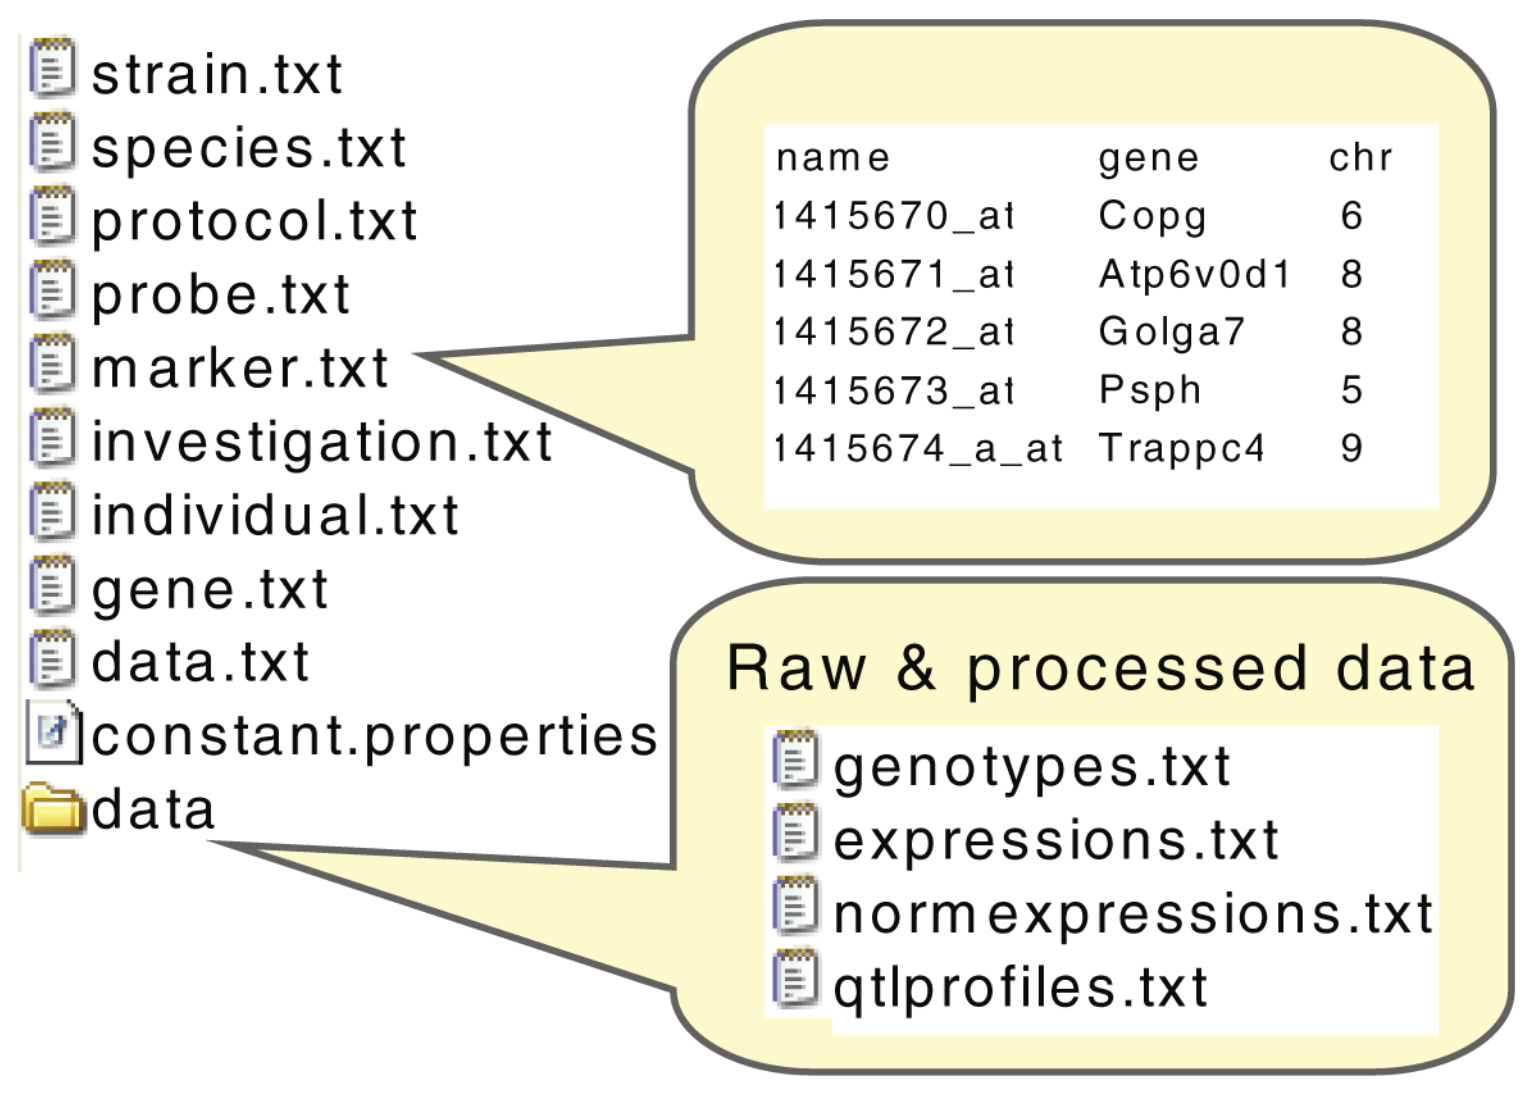
\includegraphics[width=1.0\linewidth]{img/xgap_format}
	\caption[Simple text file format]{Simple text file format. A whole investigation can be stored by using easy-to-create tabular text files for annotations or matrix-shaped text files for raw and processed data. Each ‘annotation’ file relates to one data type in the object model shown in Figure \ref{fig:xgap_model} - for example, the rows in the file ‘probe.txt’ will have the columns named in data type ‘Probe’. Each ‘data’ file contains data elements and has row names and column names referring to annotation files - for example, ‘genotypes.txt’ may refer to ‘marker.txt’ names as row names and ‘individual.txt’ names as column names. If convenient, constant values can be described in the constant.properties file such as ‘species\_name’.}
	\label{fig:xgap_format}
\end{figure}

After proving its value in several proprietary projects, a growing array of public data sets are now available at\cite{xgap_datasets} demonstrating the use of XGAP-TAB\cite{Heap_2009, Bystrykh_2005, Li_2006, Keurentjes_2007, Stranger_2007b, Myers_2007}.

\section{Easy to customize software infrastructure}
A pilot software infrastructure is available at\cite{xgap_url} to help genotype-to-phenotype researchers to adopt XGAP as a backbone for their data and tool integration.
We chose to use the MOLGENIS toolkit (biosoftware generator for MOLecular GENetics Information Systems; see Materials and methods) to auto-generate from the XGAP model: 1, an SQL (Structured Query Language for relational databases) file with all necessary statements for setting up your own, customized variant of the XGAP database; 2, application programming interfaces (APIs) in R, Java and Web Services that allow bioinformaticians to plug-in their R processing scripts, Taverna workflows\cite{Smedley_2008, xgap_taverna, Hull_2006} and other tools; 3, a bespoke web-based graphical user interface (GUI) by which researchers can submit and retrieve data and run plugged-in tools; and 4, import/export wizards to (un)load and validate data sets exchanged in XGAP-TAB format.
The auto-generation process can be repeated to quickly customize XGAP from an extended model, for example, to accommodate a particular new type of measurement technology or experimental design.

\subsection{Graphical user interface}
Figure \ref{fig:xgap_gui} shows the GUI to upload, manage, find and download genotype and phenotype data to the database.
The GUI is generated with a uniform ‘look-and-feel’, thereby lowering the barrier for novice users.
Investigations can be described with all subjects, traits, data and protocol applications involved (1).
(The numbers refer to steps in the figure.)
Data can be entered using either the edit boxes or using menu-option ‘file$|$upload’ (2).
This option enables upload of whole lists of traits and subjects from a simple tab-delimited format (3), which can easily be produced with Excel or R; MOLGENIS automatically generates online documentation describing the expected format (4).
Subsequently, the protocol applications involved can be added with the resulting raw data (for example, genetic fingerprints, expression profiles) and processed data (for example, normalized profiles, QTL profiles, metabolic networks).
These data can be uploaded, again using the common tab-delimited format or custom parsers (5) that bioinformaticians can ‘plug-in’ for specific file formats (for example, Affymetrix CEL files).
The software behind the GUI checks the relationships between subjects, traits, and data elements so no ‘orphaned’ data are loaded into the database - for example, genetic fingerprint data cannot be added before all information is uploaded on the markers and subjects involved.
Standard paths through the data upload process are employed to ensure that only complete and valid data are uploaded and to provide a consistent user experience.

\begin{figure}
	\includegraphics[width=1.0\linewidth]{img/xgap_gui}
	\caption[Graphical User Interfaces]{Graphical User Interfaces. A user interface enables biologists to add and retrieve data and run integrated tools. Genotype and phenotype information can be explored by investigation, subjects, traits or data. Hyperlinks following cross-references of the object model point to related information. Items indicated by 1-9 are described in the main text. See Table \ref{table:xgap_gui_usecases} for uses of this GUI. See also our online demonstrator at\cite{xgap_url}.}
	\label{fig:xgap_gui}
\end{figure}

Biologists can use the graphical user interface to navigate and retrieve available data for analysis.
They can use the advanced search options (6) to find certain traits, subjects, or data.
Using menu option ‘file|download’ (7) they can download visible/selected (8) data as tab-delimited files to analyze them in third party software.
Bioinformaticians can ‘plug-in’ a custom-built screen (see ‘customization’ section) that allows processing of selected data inside the GUI, for example, visualizing a correlation matrix as a graph (9) without the additional steps of downloading data and uploading it into another tool.
Biologists can create link-outs to related information, for example, to probes in GeneNetwork.org (not shown).
Table \ref{table:xgap_gui_usecases} summarizes use cases of the graphical user interface.

\begin{table}
\begin{tabulary}{\linewidth}{L}
  \hline
  Navigate all \textsl{Investigations}, and for each \textsl{Investigation}, see the \textsl{Assays} and available \textsl{Data}\\
  ~\\
  Select a \textsl{Gene} and find all \textsl{Investigations} in which this \textsl{Gene} is regulated as suggested by significant eQTL \textsl{Data} (\textsl{P}-value $<$ 0.001)\\
  ~\\
  For a given \textsl{Locus}, select all \textsl{Genes} that have QTL \textsl{Data} mapping ‘in \textsl{trans}’; and this may be regulated by this \textsl{Locus}, for example, absolute(QTL locus - gene locus) $>$ 10 Mb and QTL \textsl{P}-value $<$ 0.001\\
  ~\\
  Download a selection of raw gene expression \textsl{Data} as a tab-delimited file (to import into other software)\\
  ~\\
  Upload \textsl{Investigation} information from tab-delimited files\\
  ~\\
  Upload Affymetrix \textsl{Assays} using custom *.CEL/*.CDF file readers\\
  ~\\
  Plot highly correlated metabolic network \textsl{Data} in a network visualization graph\\
  ~\\
  Define security levels for \textsl{Assays/Investigations} to ensure that appropriate data can be viewed only by collaborators, and not by other people\\
  ~\\
  A \textsl{MassPeak} has been identified to be ‘proline’ and we can follow the link-out \textsl{URI} to Pubchem\cite{xgap_pubchem}, because it was annotated to have ‘cid’ 614, to find information on structure, activity, toxicology, and more\\
  \hline
\end{tabulary}
\caption[Use cases of the graphical user interface]{Use cases of the graphical user interface for biologists.}
\label{table:xgap_gui_usecases}
\end{table}

\subsection{Application programming interfaces}
\textsl{De facto} standard analysis tools are emerging, for example, tools for transcript data\cite{Carey_2006, Alberts_2007, Broman_2003} or metabolite abundance data\cite{Fu_2007} to mention just a few.
These tools are typically implemented using the open source software for statistical analysis and graphics named R\cite{Ihaka_1996}.
Bioinformaticians can connect their particular R or Java programs to the XGAP database using an API with similar functionality to the GUI, that is, using simple commands like ‘find’, ‘add’ and ‘update’ (R/API, Java/API).
Scripts in other programming languages and workflow tools like Taverna\cite{Hull_2006} can use web services (SOAP/API) or a simple hyperlink-based interface (HTTP/API), for example, \url{http://my-xgap/api/find/Data?investigation=1} returns all data in investigation ‘1’.
On top of this, conversion tools have been added to the R interface to read and write XGAP data to the widely used R/qtl package\cite{Broman_2003}.

Figure \ref{fig:xgap_rapi} demonstrates how researchers can use the R/API to download (or upload) all trait/subject/data involved in their investigation from (or to) their XGAP database for (after) analysis in R.
When XGAP is customized with additional data type variants, the APIs are automatically extended in the XGAP database instances by re-running the MOLGENIS generator, thus also allowing interaction with new data types in a uniform way.
These new types can then be used as standard parameters for new analysis software written in R and Java.
Table \ref{table:xgap_api_usecases} summarizes use of the application programming interface.

\begin{figure}
	\includegraphics[width=1.0\linewidth]{img/xgap_rapi}
	\caption[Application programming interfaces]{Application programming interfaces. APIs enable bioinformaticians to integrate data and tools with XGAP using web services, R-project language, Java, or simple HTTP hyperlinks. The figure shows how scientists can use the R/API to upload raw investigation data (Scientist A) so another researcher can download these data and immediately use it for the calculation of QTL profiles and upload the results thereof back to the XGAP database for use by another collaborator (Scientist B). Note how ‘add.datamatrix’ enables flexible upload of matrices for any \textsl{Subject} or \textsl{Trait} combination; this function adds one row to \textsl{Data} for each matrix, and as many rows to \textsl{DataElement} as the matrix has cells. See Table \ref{table:xgap_api_usecases} for uses of these APIs.}
	\label{fig:xgap_rapi}
\end{figure}

\begin{table}
\begin{tabulary}{\linewidth}{L}
  \hline
  In R, parse a set of tab-delimited \textsl{Marker}, \textsl{Genotype} and \textsl{Trait} files and load them into the database (R/API)\\
  ~\\
  In R, retrieve all \textsl{Trait}, \textsl{Markers}, expression \textsl{Data}, and genotype \textsl{Data} from an investigation as data matrices, before QTL mapping with MetaNetwork (R/API)\\
  ~\\
  In Java, retrieve a list of QTL profile correlation \textsl{Data} to show them as a regulatory network graph (J/API)\\
  ~\\
  In Java, customize generated file readers to load specific file formats (J/API)\\
  ~\\
  In Taverna, retrieve \textsl{Genes} from XGAP to find pathway information in KEGG (WS/API)\\
  ~\\
  In Python, retrieve a list of QTL mapping \textsl{Data} using a hyperlink to XGAP (HTTP/API)\\
  \hline
  {\footnotesize KEGG: Kyoto Encyclopedia of Genes and Genomes.}\\
\end{tabulary}
\caption[Use cases of the application programming interface]{Use cases of the application programming interface for bioinformaticians}
\label{table:xgap_api_usecases}
\end{table}

\subsection{Import/export wizards}
A generated import tool takes care of checking the consistency of all traits, subjects and data that are provided in XGAP-TAB text files and loads them into the database.
The entries in all files should be correctly linked, the data must be imported in the right order and the names and IDs need to be resolved between all the annotation files to check and link genes, microarray probes and gene expression to the data.
The import program takes care of all these issues (conversion, relationship checks, dependency ordering, and so on).
Moreover, the import program supports ‘transactions’, which ensures that all data inserts are rolled back if an import fails halfway, preventing incomplete or incorrect investigation data to be stored in the database.
In a similar way, an export wizard is provided to download investigation data as a zipped directory of XGAP-TAB files.

When XGAP is customized with additional data type variants, the import/export program is automatically extended by the MOLGENIS generator, ‘future-proofing’ the data format for new biotechnological profiling platforms.
Moreover, the auto-generated import program can also be used as a template for parsers of proprietary data formats, such as implemented in parsers for the PED/MAP, HapMap, and GeneNetwork data.
Collaborations are underway within EBI and GEN2PHEN to also enable import/export of MAGE-TAB\cite{Rayner_2006} files, the standard format for microarray experiments, of PAGE-OM\cite{xgap_pageom} files, a specialized format for genome-variation oriented genotype-to-phenotype experiments, and of ISA-TAB\cite{xgap_gen2phen} files, a generalized evolution of MAGE-TAB to represent all experimental metadata on any investigation, study and assay designed to be FuGE compatible.
Also, convertors to ease retrieval and submission to public repositories like dbGaP are under development.
It is envisaged that integration of all these formats will enable integrated analysis of experimental data from, for example, mouse and human experiments using various biotechnology platforms, which was previously near impossible for biological labs to implement.

\subsection{Customizing XGAP}
Customizations and extensions of the XGAP object model can be described in a single text file using MOLGENIS\cite{Swertz_2007, Swertz_2004} DSL.
On the push of a button, the MOLGENIS generator instantly produces an extended version of the XGAP database software from this DSL file.
A regression test procedure assists XGAP developers to ensure their extensions do not break the XGAP exchange format.
Figure \ref{fig:xgap_custom}a shows how the addition of a \textsl{Metabolite} data entity as a new variant of \textsl{Trait} takes only a few lines in this DSL.
Figure \ref{fig:xgap_custom}b shows how the GUI can be customized to suit a particular experimental process.
Figure \ref{fig:xgap_custom}c shows how programmers can add a ‘plug-in’ program that is not generated by MOLGENIS but written by hand in Java (for example, a viewer that plots QTL profiles interactively).
Moreover, use of Cascading Style Sheets (CSS) enables research projects to completely customize the look and feel of their XGAP.

\begin{figure}
	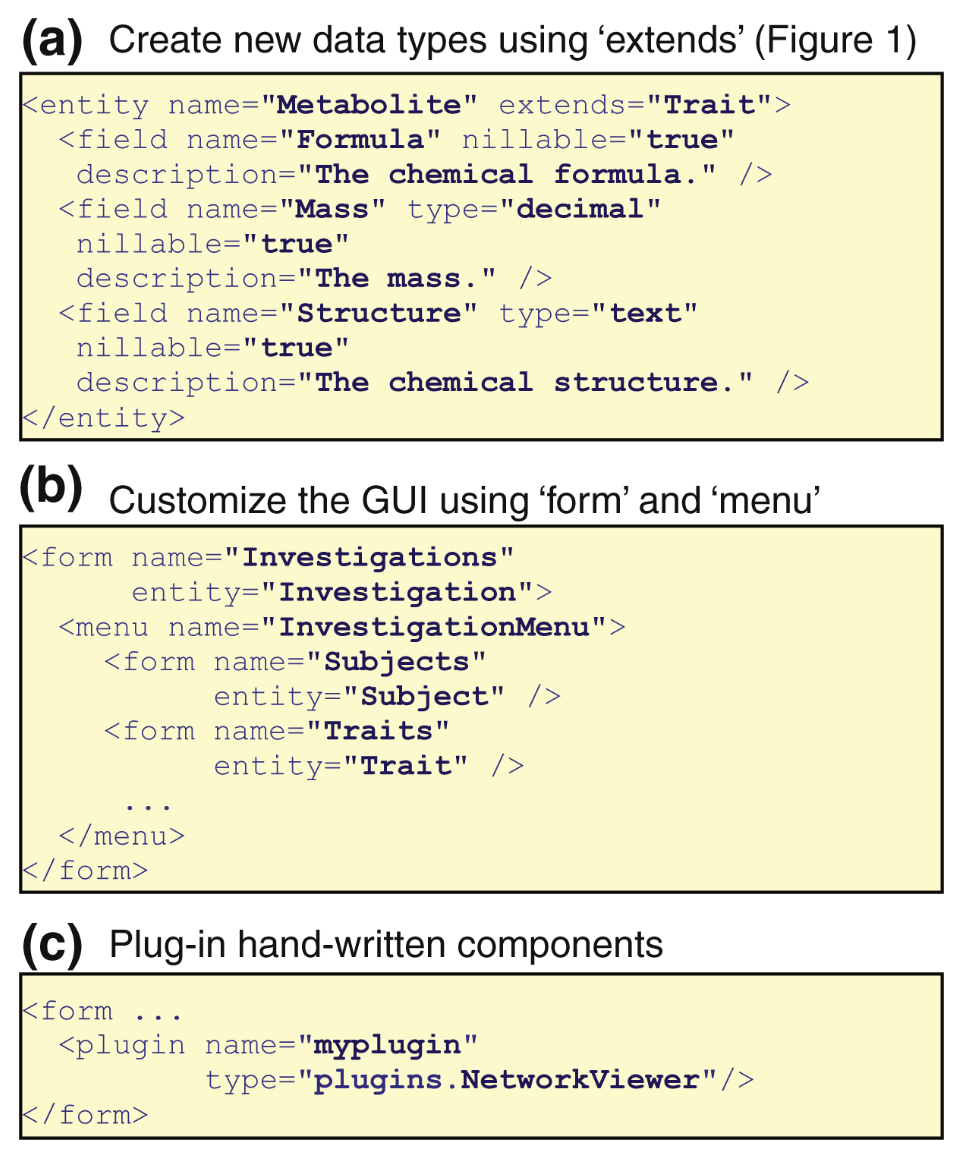
\includegraphics[width=0.97\linewidth]{img/xgap_custom}
	\caption[Customizing XGAP]{Customizing XGAP. A file in MOLGENIS domain-specific language is used to describe and customize the XGAP database infrastructure in a few lines. \textbf{(a)} Shows how the addition of a \textsl{Metabolite} data entity as a new variant of \textsl{Trait} takes only a few lines in this DSL. \textbf{(b)} Shows how the GUI can be customized to suit a particular experimental process. \textbf{(c)} Shows how programmers can add a ‘plug-in’ program that is not generated by MOLGENIS but written by hand in Java.}
	\label{fig:xgap_custom}
\end{figure}

All XGAP and MOLGENIS software can be downloaded for free under the terms of the open source license LGPL.
Extended documentation on XGAP and MOLGENIS customization is available online at the XGAP and MOLGENIS wikis\cite{xgap_url, xgap_molgenurl}.

\section{Conclusions}
In this paper we report a minimal and extensible data infrastructure for the management and exchange of genotype-to-phenotype experiments, including an object model for genotype and phenotype data (XGAP-OM), a simple file format to exchange data using this model (XGAP-TAB) and easy-to-customize database software (XGAP-DB) that will help groups to directly use and adapt XGAP as a platform for their particular experimental data and analysis protocols.

We successfully evaluated the XGAP model and software in a broad range of experiments: array data (gene expression, including tiling arrays for detection of alternative splicing, ChIP-on-chip for methylation, and genotyping arrays for SNP detection); proteomics and metabolomics data (liquid chromatography time of flight mass spectrometry (LC-QTOF MS), NMR); classical phenotype assays\cite{Heap_2009, Bystrykh_2005, Li_2006, Keurentjes_2006, Stranger_2007b, Myers_2007, Bailey_2008, Beamer_1999}; other assays for detection of genetic markers; and annotation information for panel, gene, sample and clone.
Nontechnical partners successfully evaluated the practical utility by independently formatting and loading parts of their consortium data: EU-CASIMIR (for mouse; Table \ref{table:xgap_consortia}), EU-GEN2PHEN (for human; Table \ref{table:xgap_consortia}), EU-PANACEA (for \textsl{C. elegans}) and IOP-Brassica (for plants).
A public subset of these data sets is available for download at\cite{xgap_url}.
When needed we could quickly add customizations to the model, building on the general schema, and then use MOLGENIS to generate a new version of the software at the push of a button, for example, to support \textsl{NMR} methods as an extended type of \textsl{Trait}\cite{Fu_2009}.
Furthermore we successfully integrated processing tools, such as a two-way communication with R/QTL\cite{Broman_2003} enabling QTL mapping on XGAP stored genotypes and phenotypes with QTL results stored back into XGAP.

\linespread{1.00} % need to squeeze a bit to fit these tables nicely

\begin{table}
\small
\begin{tabularx}{\linewidth}{ l X }
  Consortium & Remit \\
  \hline
  \rule{0pt}{2.5ex}CASIMIR & The collection and distribution of large volumes of complex data typical of functional genomics is carried out by an increasing number of disseminated databases of hugely variable scale and scope. Combined analysis of highly distributed datasets provides much of the power of the approach of functional genomics, but depends on databases’ ability to exchange data with each other and on analytical tools with semantic and structural integrity. Agreement on the standards adopted by databases will inevitably be a matter of community consensus and to that end a recent coordination action funded by the European Commission, CASIMIR\cite{xgap_casimir}, is engaged in a community consultation on the nature of the technical and semantic standards needed. What has already become clear in use-case studies conducted so far is that whatever standards are adopted, they will inevitably remain dynamic and continue to develop, particularly as new data types are collected. Crucially, they should allow the open-ended development of analytical and datamining software, while integration of efforts to agree such standards and develop new software is essential.\\
  \rule{0pt}{2.5ex}GEN2PHEN & Currently available genotype-to-phenotype (G2P) databases are few and far between, have great diversity of design, and limited or no interoperability between them. This arrangement provides no convenient way to populate the databases, no easy way to exchange, compare or integrate their content, and absolutely no way to search the totality of gathered information. In this context, the European Commission has recently funded the GEN2PHEN project\cite{xgap_gen2phen}, which intends to significantly improve the database infrastructure available within Europe for the collation, storage, and analysis of human and model-organism G2P data. This will be achieved by first developing various cutting-edge solutions, and then deploying these in conjunction with proven concepts, so as to transform the current elementary G2P database reality into a powerful networked hierarchy of interlinked databases, tools and standards.\\
  \hline
\end{tabularx}
\caption[XGAP participating consortia]{XGAP participating consortia.}
\label{table:xgap_consortia}
\end{table}

\linespread{1.05} % and back to normal

Based on these experiences, we expect use of XGAP to help the community of genome-to-phenome researchers to share data and tools, notwithstanding large variations in their research aims.
The XGAP data format can be used to represent and exchange all raw, intermediate and result data associated with an investigation, and an XGAP database, for instance, can be used as a platform to share both data and computational protocols (for example, written in the R statistical language) associated with a research publication in an open format.
We envision a directory service to which XGAP users can publish metadata on their investigations either manually or automatically by configuring this option in the XGAP administration user interface.
This directory service can then be used as an entry point for federated querying between the community of XGAPs to share data and tools.

Groups that already have an infrastructure can assimilate XGAP to ease evolution of their existing software.
Next to their existing user tools, they can ‘rewire’ algorithms and visual tools to also use the MOLGENIS APIs as data backend.
Thus, researchers still have the same features as before, plus the features provided by the generated infrastructure (for example, data management GUIs, R/API) and connected tools (for example, R packages developed elsewhere).
Moreover, much less software code needs to be maintained by hand when replacing hand-written parts by MOLGENIS-generated parts, allowing software engineers to add new features for researchers much more rapidly.

We invite the broader community to join our efforts at the public XGAP.org wiki, mailing list and source code versioning system to evolve and share the best XGAP customizations and GUI/API ‘plug-in’ enhancements, to support the growing range of profiling technologies, create data pipelines between repositories, and to push developments in the directions that will most benefit research.

\section{Materials and methods}
Software modeling, auto-generation/configuration and component toolboxes are increasingly used in bioinformatics to speed up (bespoke) biological software development; see our recent review\cite{Swertz_2007}.
For XGAP we required a software toolbox providing query interfaces, data management interfaces, programming interfaces to R and web services, simple data exchange formats and a minimal requirement of programming knowledge.
The MOLGENIS modeling language and software generator toolbox\cite{Swertz_2007, xgap_molgenurl} was chosen as it combines all these features.

Several alternative toolboxes were evaluated: BioMart\cite{xgap_molgenurl, Smedley_2009} and InterMine\cite{Lyne_2007} generate powerful query interfaces for existing data but are not suited for data management; Omixed\cite{xgap_omixed} generates programmatic interfaces onto databases, including a security layer, but lacks user interfaces; PEDRO/Pierre\cite{Jameson_2008} generates data entry and retrieval user interfaces but lacks programmatic interfaces; and general generators such as AndroMDA\cite{xgap_andromda} and Ruby-on-Rails\cite{xgap_ror} require much more programming/configuration efforts compared to tools specific to the biological domain.
Turnkey\cite{O_Connor_2008} seemed to be closest to our needs: it emerged from the GMOD community having GUI and SOAP interfaces but lacks auto-generation of R interfaces and a file exchange format.

Figure \ref{fig:xgap_generate} summarizes how MOLGENIS generates the XGAP da\-ta\-ba\-se software in three layers: database, API and GUI.
MOLGENIS either generates a high-performance ‘server’ edition, which requires installation on server software, or a limited ‘standalone’ edition that runs on a desktop computer without any additional configuration.
The database layer is generated as SQL files with ‘database CREATE statements’ that are loaded into either MySQL (server), PostgreSQL (server) or HSQLDB (standalone).
Each data type in the XGAP object model (Figure \ref{fig:xgap_model}) is mapped to its own table - for example, there is a ‘Trait’ table.
Each inheritance adds another table, for example, each \textsl{Gene} has an entry in the ‘Gene’ table and also in the ‘Trait’ table.
One-to-many crossreferences between data types are mapped as foreign keys - for example, \textsl{Data} has a numeric field called ‘Investigation’ that must refer to the \textsl{foreign key} ‘molgenisid’ of \textsl{Investigation}.
Many-to-many cross-references are mapped via a ‘link-table’ - for example, an additional table \textsl{‘mref\_import\_data’} is generated for two foreign keys to \textsl{Data} and \textsl{ProtocolApplication}, respectively, to model the \textsl{importData} relationship between them.
The API layer is generated as Java files either served via Tomcat (server) or Jetty (standalone).
A Java class is generated for each data type - for example, there is a class \textsl{Gene}.
All data can be queried programmatically via a central \textsl{Database} class, that is, command \textsl{db.find(Gene.class)} returns all \textsl{Gene} objects in the database.
To enhance performance, the API uses the ‘batched’ update methods of Java’s DataBase Connectivity (JDBC) package and the ‘multi-row-syntax’ of MySQL to allow inserts of 10,000s of data entries in a single command, an optimization that is 5 to 15 times quicker than standard one-by-one updates.
The Java/API is exposed with a SOAP/API, HTTP/API and R/API, so XGAP can also be accessed via web service tools like Taverna, HTTP or R, respectively (accessible via hyperlinks in the GUI).
The GUI layer is also generated as Java files.
The GUI includes classes for each Menu and Form - for example, the \textsl{InvestigationForm} class generates a view- and editform for investigations in the GUI.
The generation is steered from one XML file written in MOLGENIS DSL (partially shown in Figure \ref{fig:xgap_custom}).
To enable FuGE extension, the FuGE model was automatically translated into MOLGENIS DSL.
We therefore first downloaded the FuGE v1 MagicDraw file from\cite{xgap_fuge}, exported from MagicDraw to XMI 2.1, parsed the XMI using the EMF parser from Eclipse\cite{xgap_eclipse} and then automatically translated it into MOLGENIS DSL using a newly built XmiToMolgenis tool.
Compatibility with the FuGE standard is ensured via inheritance; that is, \textsl{Investigation}, \textsl{Protocol}, \textsl{ProtocolApplication}, \textsl{Data} and \textsl{DimensionElement} in XGAP all extend FuGE data types of the same name.
Further implementation details can be found at \cite{xgap_url, xgap_molgenurl}.

\begin{figure}
	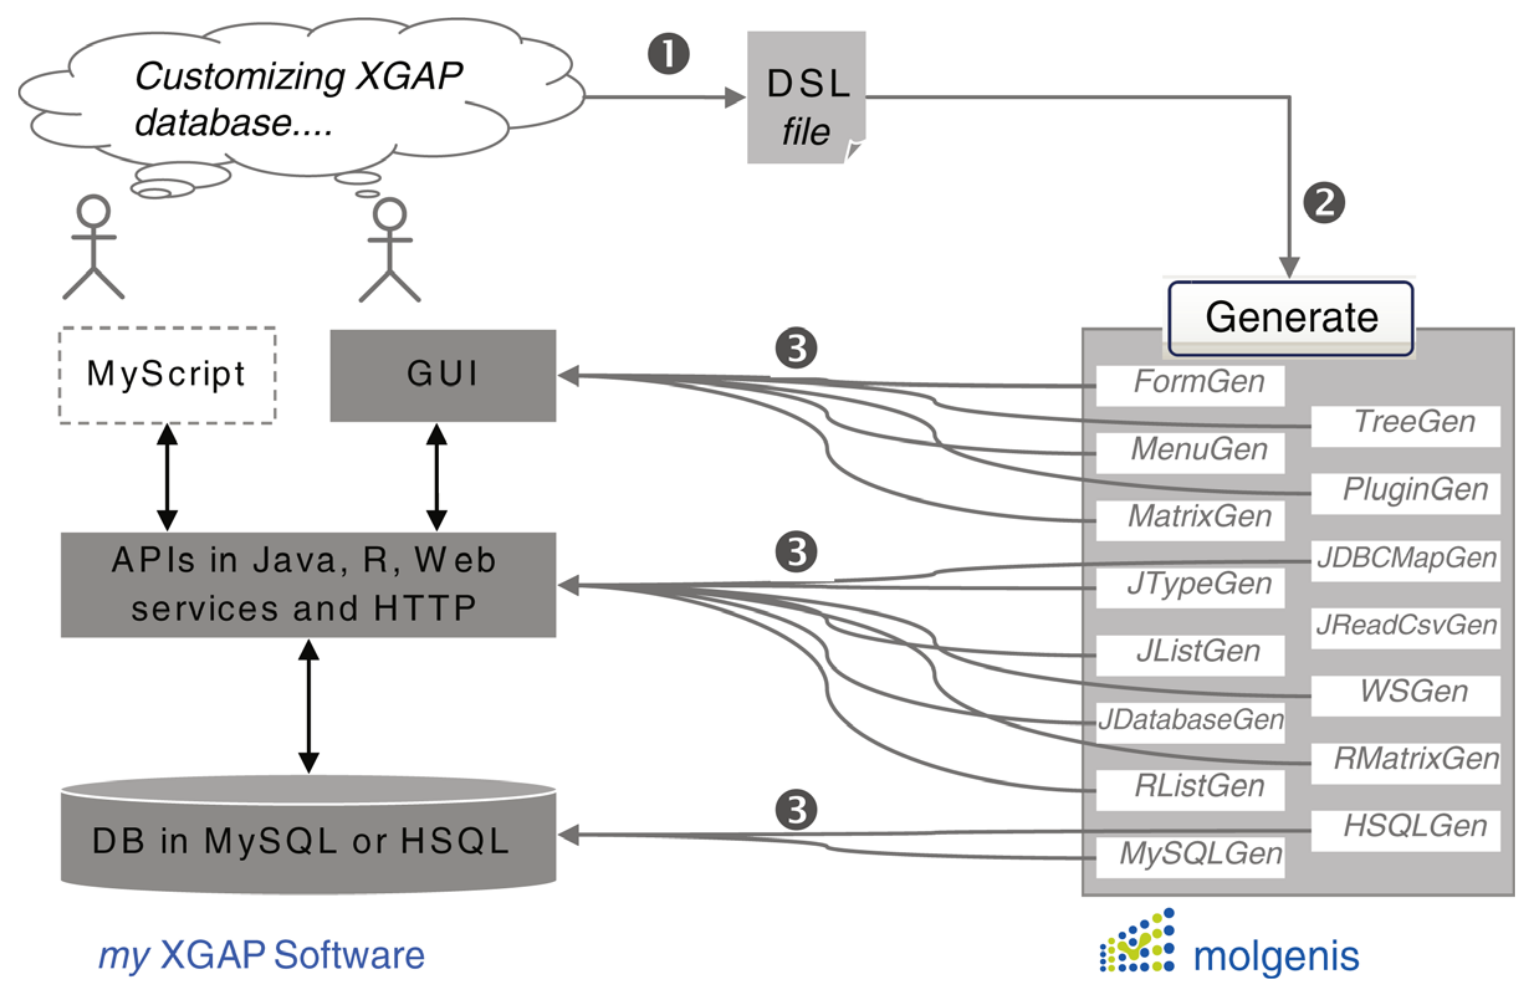
\includegraphics[width=1.0\linewidth]{img/xgap_generate}
	\caption[Auto-generation of XGAP software]{Auto-generation of XGAP software. Open source generator tools are used to produce a customized XGAP software infrastructure. 1, The XGAP object model is described using the MOLGENIS’ little modeling language (Figure \ref{fig:xgap_rapi}). 2, Central software termed MolgenisGenerate runs several generators, building on the MOLGENIS catalogue of reusable assets. 3, At the push of the button, the software code for a working XGAP implementation is automatically generated from the DSL file. GUI and APIs provide simple tools to add and retrieve data, while the reusable assets of MOLGENIS hide the complexity normally needed to implement such tools. For customization, only simple changes to the XGAP model file are required; the MOLGENIS generator takes care of rewriting all the necessary files of SQL and Java software code, saving time and ensuring a consistent quality.}
	\label{fig:xgap_generate}
\end{figure}

\subsection*{Abbreviations}
API: application programming interface; dbGaP: database of genotypes and phenotypes; DSL: domain-specific computer language; FuGE: Functional Genomics Experiment model; GMOD: Generic Model Organism Database; GUI: graphical user interface; LC/MS: liquid chromatography-mass spectrometry; MAGE-TAB: tabular format for microarray gene expression experiments; MOLGENIS: biosoftware generator for MOLecular GENetics Information Systems; NMR: proton nuclear magnetic resonance; QTL: quantitative trait locus; SOAP: web services using simple object access protocol; SQL: Structured Query Language for relational databases; XGAP: eXtensible Genotype And Phenotype platform.

\subsection*{Acknowledgements}
The authors thank CASIMIR (funded by the European Commission under contract number LSHG-CT-2006-037811,\cite{xgap_casimir}; Table \ref{table:xgap_consortia}), and GEN2PHEN, a FP7 project funded by the European Commission (FP7-HEALTH contract 200754,\cite{xgap_gen2phen}; Table \ref{table:xgap_consortia}).
The authors also thank NWO (Rubicon Grant 825.09.008) for financial support.

\subsection*{Authors’ contributions}
MAS, ARJ, PS, KS, JMH, DS, EOB, HEP and RCJ compiled the functional requirements for the XGAP community platform and drafted the extensible data model.
MAS, KJV, BMT, RAS, and MD refined and implemented the model using MOLGENIS, and added all parsers, and user interfaces.
MAS and KW implemented Taverna compatible web services and GV, DA, KJV and MS implemented R-services.
MAS, HEP and RCJ drafted the manuscript.
All authors evaluated XGAP components in various settings.
All authors read and approved the final manuscript.

\chapter[A scalable web environment for multi-level QTL analysis]{xQTL workbench: A scalable web environment for multi-level QTL analysis}
\chaptermark{A web environment for QTL analysis}
\label{chap:xqtl}

{ \Large \leftwatermark{
\put(-67,-66.5){ 1 }
\put(-67,-91.5){ 2 }
\put(-76.5,-125){\includegraphics[scale=0.8]{img/thumbindex.eps}} \put(-67,-116.5){ {\color{white} 3 }}
\put(-67,-141.5){ 4 }
\put(-67,-166.5){ 5 }
\put(-67,-191.5){ 6 }
\put(-67,-216.5){ 7 }
\put(-67,-241.5){ 8 }
} \rightwatermark{
\put(350.5,-66.5){ 1 }
\put(350.5,-91.5){ 2 }
\put(346.5,-125){\includegraphics[scale=0.8]{img/thumbindex.eps}} \put(350.5,-116.5){ {\color{white} 3 }}
\put(350.5,-141.5){ 4 }
\put(350.5,-166.5){ 5 }
\put(350.5,-191.5){ 6 }
\put(350.5,-216.5){ 7 }
\put(350.5,-241.5){ 8 }
}}

\hfill \underline{Bioinformatics.} 2012 Apr 1;28(7):1042-4.

\hfill DOI: \href{https://doi.org/10.1093/bioinformatics/bts049}{10.1093/bioinformatics/bts049}

\hfill PubMed ID: \href{https://www.ncbi.nlm.nih.gov/pubmed/22308096}{22308096}

\newpage

\noindent
Danny Arends\textsuperscript{1,†}, K. Joeri van der Velde\textsuperscript{1,†}, Pjotr Prins\textsuperscript{1,2}, Karl W. Broman\textsuperscript{3}, Steffen Möller\textsuperscript{4}, Ritsert C. Jansen\textsuperscript{1} and Morris A. Swertz\textsuperscript{1,5,6,*}\\

\noindent
1. Groningen Bioinformatics Centre, University of Groningen, Groningen.\\
2. Laboratory of Nematology, Wageningen University, Wageningen, The Netherlands.\\
3. Department of Biostatistics and Medical Informatics, University of Wisconsin-Madison, Madison, WI, USA.\\
4. Institut für Neuro- und Bioinformatik, Universität zu Lübeck.\\
5. Genomics Coordination Centre, University Medical Centre Groningen, University of Groningen, The Netherlands.\\
6. EMBL-EBI, the European Bioinformatics Institute, Hinxton, UK.\\

\noindent
Associate Editor: Jeffrey Barrett
\\~\\
Received on September 30, 2011; revised on December 19, 2011; accepted on January 20, 2012
\\~\\
* To whom correspondence should be addressed.\\
† The authors wish it to be known that, in their opinion, the first two authors should be regarded as joint First Authors.

\section*{Abstract}
\textbf{Summary:} \textsl{x}QTL workbench is a scalable web platform for the mapping of quantitative trait loci (QTLs) at multiple levels: for example gene expression (eQTL), protein abundance (pQTL), metabolite abundance (mQTL) and phenotype (phQTL) data. Popular QTL mapping methods for model organism and human populations are accessible via the web user interface. Large calculations scale easily on to multi-core computers, clusters and Cloud. All data involved can be uploaded and queried online: markers, genotypes, microarrays, NGS, LC-MS, GC-MS, NMR, etc. When new data types come available, \textsl{x}QTL workbench is quickly customized using the Molgenis software generator.\\
\textbf{Availability:} \textsl{x}QTL workbench runs on all common platforms, including Linux, Mac OS X and Windows. An online demo system, installation guide, tutorials, software and source code are available under the LGPL3 license from \url{http://www.molgenis.org/xqtl}\footnote{The URL in the original paper is no longer active and was updated here.}.\\
\textbf{Contact:} m.a.swertz@rug.nl

\section{Introduction}
Modern high-throughput technologies generate large amounts of genomic, transcriptomic, proteomic and metabolomic data. However, existing open source web-based tools for QTL analysis, such as webQTL \cite{Wang_2003} and QTLNetwork \cite{Yang_2008}, are not easily extendable to different settings and computationally scalable for whole genome analyses. \textsl{x}QTL workbench makes it easy to analyse large and complex datasets using state-of-the-art QTL mapping tools and to apply these methods to millions of phenotypes using parallelized ‘Big Data’ solutions \cite{Trelles_2011}. \textsl{x}QTL workbench also supports storing of raw, intermediate and final result data, and analysis protocols and history for reproducibility and data provenance. Use of Molgenis \cite{Swertz_2010a} helps to customize the software. All is conveniently accessible via standard Internet browsers on Windows, Linux or Mac (and using Java, R for the server).

\section{Features}
\textsl{x}QTL workbench provides visualization of QTL profiles, single and multiple QTL mapping methods, easy addition of new QTL analyses, scalable data management and analysis tracking.

\subsection{Explore QTL profiles}
Through the web interface, users can explore mapped QTLs, and underlying information by viewing QTL plots in an interactive scrollable and zoomable window. \textsl{x}QTL workbench has support for other common image formats, such as PNG, JPG, SVG and embedded postscript; useful for publishing scientific results online, and on paper. From the output, main database identifiers, such as gene, protein and/or metabolite identifiers are automatically linked-out to matching external web pages of public database such as NCBI, KEGG and Wormbase.

\subsection{Single and multiple QTL mapping}
\textsl{x}QTL workbench wraps R/qtl \cite{Arends_2010, Broman_2003} in a web-based analysis framework offering all important QTL mapping routines, such as the EM algorithm, imputation, Haley-Knott regression, the extended Haley-Knott method, marker regression and Multiple QTL mapping. In addition, \textsl{x}QTL workbench includes R/qtlbim, a library that provides a Bayesian model selection approach for mapping multiple interacting QTL \cite{Yandell_2007} and Plink, a library for association QTL mapping on single nucleotide polymorphisms (SNP) in natural populations \cite{Purcell_2007}.

\subsection{Add new analysis tools}
\textsl{x}QTL workbench supports flexible adding of more QTL analysis software: any R-based, or command-line tool, can be plugged in. All analysis results are uploaded, stored and tracked in the \textsl{x}QTL workbench database through an R-API. When new tools are added, they can build on the high-level multi-core computer, cluster and Cloud management functions, based on TORQUE/OpenPBS and BioNode \cite{Prins_2012}. \textsl{x}QTL workbench can be made part of a larger analysis pipeline using interfaces to R, Excel, REST and SOAP web services and Galaxy \cite{Goecks_2010}.


\begin{figure}
	\centering
	\includegraphics[scale=0.33]{img/xqtl_overview}
	\caption[Screenshot of xQTL workbench with all features]{Screenshot of \textsl{x}QTL workbench with all features enabled; (1) import phenotype, genotype and genetic map data, examples are given per import type; (2) search through the whole database, explore and browse your data using molgenis generated web-interfaces; (3) run R/qtl QTL mapping, the general plugin allows users to perform not only QTL mapping but also other analyze; (4) use default (or custom) plugins to explore results (e.g. Heatmaps, QTL profiles); (5) add new tools to the workbench (for Bio informaticians); (6) user management and access control of the system (Only for admins); (7) expert settings can be altered in the admin tab (Only for admins); (8) connect/share data using generated API’s to R statistics, REST/JSON, SOAP.}
		\label{fig:xqtl_overview}
\end{figure}

\subsection{Track analysis and monitor performance}
When a new analysis protocol or R script is defined, this protocol can easily be applied to new data. Also, \textsl{x}QTL workbench keeps track of history. Re-use of analysis protocols can be done in an automated fashion. Previous analyses can be rerun without resetting parameters. \textsl{x}QTL workbench provides an online overview of past analyses e.g. which analyses were performed, by who, when and display settings applied.

\subsection{Scalable data management}
\textsl{x}QTL workbench has a consistency checking database based on XGAP specification \cite{Swertz_2010b}, user interfaces to manage and query genotype and phenotype datasets and support for various database back-ends including HSQL (standalone) and MySQL. Phenotype, genotype and genetic map data can be imported as text (TXT), comma separated (CSV) and Excel files. \textsl{x}QTL workbench handles and stores large data in a new and efficient binary edition of the XGAP format, named XGAPbin (extension .xbin), documented online. Such binary formats are essential when handling, storing and transporting multi-Gigabyte datasets.

\subsection{Customizable to research needs}
Additional modules for new data modalities can be added using Molgenis software generator \cite{Swertz_2010b}.
The ‘look and feel’ of \textsl{x}QTL workbench is adaptable to institute or consortium style by changing a simple template, which is described in the \textsl{x}QTL workbench documentation enabling seamless integration into an existing website or intranet site, such as recently for EU-PANACEA model organism project and LifeLines biobank.

\section{Implementation}
We built \textsl{x}QTL workbench on top of Molgenis \cite{Swertz_2004}, a Java-based software to generate tailored research infrastructure on-demand \cite{Swertz_2007}. From a single ‘blueprint’ describing the whole system, Molgenis auto-generates a full application including user interface, database infrastructure, application programming interfaces in R, REST and SOAP (APIs). Molgenis' flexibility and robustness is proven by the wide range of research projects, e.g. the Nordic GWAS Control database \cite{Leu_2010}, EB mutation database \cite{van_den_Akker_2011} and the Animal observation database \cite{Swertz_2010a}.

For data storage, the eXtensible Genotype and Phenotype (XGAP) data model was adopted \cite{Swertz_2010b} and extended for big data. To support the increased demand for computational resources for included mapping routines, we added high-level cluster and cloud management functions for computation. The scalable QTL mapping routines of \textsl{x}QTL workbench are written in R and C. The choice of R ties in with the general practice of using R for QTL mapping. The user interface includes direct access to the R interpreter. Both \textsl{x}QTL workbench and Molgenis are open-source software, and source code is transparently stored and tracked in online source control repositories.

\section{Conclusion}
\textsl{x}QTL workbench provides a total solution for web-based analysis: major QTL mapping routines are integrated for use by experienced and inexperienced users.
Researchers can upload raw data, run analyses, explore mapped QTL and underlying information, and link-out to important databases.
New algorithms can be flexibly added, immediately available to all users. Large analyses can be easily executed on a cluster or in the Cloud.
Future work include visualizations and search options to explore the results.
We also had an EU-SYSGENET workshop that envisioned further integration of \textsl{x}QTL with analysis tools like HAPPY, databases like GeneNetwork, and the workflow manager TIQS \cite{Durrant_2011}.

\section*{Acknowledgements}
We thank Konrad Zych for Figure \ref{fig:xqtl_overview}.
\\~\\
\textsl{Funding}: National Institutes of Health (GM074244 to KB); Netherlands Organisation for Scientific Research (NWO)/TTI Green Genetics (1CC029RP to P.P.); NWO (Rubicon 825.09.008 to M.A.S), Centre for BioSystems Genomics (CBSG), Netherlands Consortium of Systems Biology (NCSB) (to D.A.), Netherlands Bioinformatics Center (NBIC) (to M.A.S.), all part of Netherlands Genomics Initiative/NWO; Target/LifeLines co-funded by the European Regional Development Fund and NWO (to M.A.S.); and EU-FP7 Projects PANACEA (222936 to K.J.v.d.v.) and EURATRANS (241504 to R.C.J.).
\\~\\
\textsl{Conflict of Interest}: none declared.





\chapter[A web database for linking human disease to \textsl{C. elegans}]{WormQTL\textsuperscript{HD}: A web database for linking human disease to natural variation data in ~~~~~~~~~~~~~~~~~~ \textsl{C. elegans}}
\chaptermark{Linking human disease to \textsl{C. elegans}}
\label{chap:wormqtl}

{ \Large \leftwatermark{
\put(-67,-66.5){ 1 }
\put(-67,-91.5){ 2 }
\put(-67,-116.5){ 3 }
\put(-76.5,-150){\includegraphics[scale=0.8]{img/thumbindex.eps}} \put(-67,-141.5){ {\color{white} 4 }}
\put(-67,-166.5){ 5 }
\put(-67,-191.5){ 6 }
\put(-67,-216.5){ 7 }
\put(-67,-241.5){ 8 }
} \rightwatermark{
\put(350.5,-66.5){ 1 }
\put(350.5,-91.5){ 2 }
\put(350.5,-116.5){ 3 }
\put(346.5,-150){\includegraphics[scale=0.8]{img/thumbindex.eps}} \put(350.5,-141.5){ {\color{white} 4 }}
\put(350.5,-166.5){ 5 }
\put(350.5,-191.5){ 6 }
\put(350.5,-216.5){ 7 }
\put(350.5,-241.5){ 8 }
}}

\hfill \underline{Nucleic Acids Res.} 2014 Jan;42(Database issue):D794-801.

\hfill DOI: \href{https://doi.org/10.1093/nar/gkt1044}{10.1093/nar/gkt1044}

\hfill PubMed ID: \href{https://www.ncbi.nlm.nih.gov/pubmed/24217915}{24217915}

\newpage

\noindent
K. Joeri van der Velde\textsuperscript{1,2,3}, Mark de Haan\textsuperscript{1,2,3,4}, Konrad Zych\textsuperscript{2}, Danny Arends\textsuperscript{2},
L. Basten Snoek\textsuperscript{5}, Jan E. Kammenga\textsuperscript{5}, Ritsert C. Jansen\textsuperscript{2}, Morris A. Swertz\textsuperscript{1,2,3,*} and Yang Li\textsuperscript{2,3,*}\\

\noindent
1. Genomics Coordination Center, University of Groningen, University Medical Center Groningen, P.O. Box 30001, 9700 RB Groningen, The Netherlands.\\
2. Groningen Bioinformatics Center, University of Groningen, P.O. Box 11103, 9700 CC Groningen, The Netherlands.\\
3. Department of Genetics, University of Groningen, University Medical Center Groningen, P.O. Box 30001, 9700 RB Groningen, The Netherlands.\\
4. Department of Bioinformatics, Hanze University of Applied Sciences, Groningen, Zernikeplein 11, 9747 AS, The Netherlands.\\
5. Laboratory of Nematology, Wageningen University, 6708 PB Wageningen, The Netherlands.\\

\noindent
Received August 14, 2013; Revised October 9, 2013; Accepted October 10, 2013
\\~\\
*To whom correspondence should be addressed. Tel: +31 50 367100; Fax: +31 50 361 7230; Email: m.a.swertz@rug.nl\\
Correspondence may also be addressed to Yang Li. Tel: +31 50 367100; Fax: +31 50 361 7230; Email: yang.li@rug.nl
\\~\\
The authors wish it to be known that, in their opinion, the first two authors should be regarded as Joint First Authors.

\section*{Abstract}
Interactions between proteins are highly conserved across species.
As a result, the molecular basis of multiple diseases affecting humans can be studied in model organisms that offer many alternative experimental opportunities.
One such organism ---\textsl{Caenorhabditis elegans}--- has been used to produce much molecular quantitative genetics and systems biology data over the past decade.
We present WormQTL\textsuperscript{HD} (Human Disease), a database that quantitatively and systematically links expression Quantitative Trait Loci (eQTL) findings in \textsl{C. elegans} to gene-disease associations in man.
WormQTL\textsuperscript{HD}, available online at \url{http://www.wormqtl-hd.org}, is a user-friendly set of tools to reveal functionally coherent, evolutionary conserved gene networks.
These can be used to predict novel gene-to-gene associations and the functions of genes underlying the disease of interest.
We created a new database that links \textsl{C. elegans} eQTL data sets to human diseases (34,337 gene-disease associations from OMIM, DGA, GWAS Central and NHGRI GWAS Catalogue) based on overlapping sets of orthologous genes associated to phenotypes in these two species.
We utilized QTL results, high-throughput molecular phenotypes, classical phenotypes and genotype data covering different developmental stages and environments from WormQTL database.
All software is available as open source, built on MOLGENIS and xQTL workbench.

\section{Introduction}
Many exciting data sets have been collected in recent years for \textsl{Cae\-nor\-hab\-di\-tis elegans}, a free-living, non-parasitic soil-related nematode that feeds on the bacteria of decaying organic matter.
This worm has many useful features that have made it one of the most studied model organisms: it is small and easy to house, has a short generation time and is transparent.
As a consequence, its genomic information is now available \cite{The_C_nbsp_elegans_Sequencing_Consortium_1998}, and the developmental path and function of almost every cell in its body has been described \cite{Gerstein_2010}.
In addition, recent genetical genomics studies in \textsl{C. elegans} have revealed thousands of genomic regions (loci) that are associated to the quantitative variation in a diverse range of phenotypes, such as gene expression [expression Quantitative Trait Loci (eQTLs)] \cite{Gaertner_2010,Kammenga_2008,Palopoli_2008,Li_2010,Vinuela_2010,Vinuela_2012,Rockman_2010}, lifespan \cite{Doroszuk_2009}, development \cite{Gutteling_2007,Gutteling_2006,Kammenga_2007}, stress resistance \cite{Rodriguez_2012,Harvey_2008}, behaviour \cite{McGrath_2009,Reddy_2009}, dauer formation \cite{Harvey_2008,Green_2013a} and sensitivity to RNAi treatments \cite{Elvin_2011}.

Genes having eQTLs mapping to the same genomic region (i.e. hotspot) are possibly involved in the same biological pathway/process. Palopoli \textsl{et al.} \cite{Palopoli_2008} have shown that biochemical processes and molecular functions of genes are generally highly conserved.
Lee \textsl{et al.} \cite{Lee_2008} have shown that using the OMIM database \cite{Hamosh_2000} (\url{http://omim.org/}) and orthologue mapping data from INPARANOID \cite{Ostlund_2009}, it is possible to infer new gene-gene interactions that are responsible for a certain disease in man from model organism data.
McGary \textsl{et al.} \cite{McGary_2010} have shown that the conservation level between \textsl{C. elegans} and man is sufficient to infer gene-gene interactions in man from worm data.
Even though the global disease phenotypes may not be at all comparable, the molecular basis may be common (e.g. breast cancer and high male incidence of progeny).
For example, research on stress response in \textsl{C. elegans} has provided detailed insight into the genetic and molecular mechanisms underlying complex human diseases \cite{Rodriguez_2013}.
In addition, Shaye and Greenwald \cite{Shaye_2011} have generated a compendium of \textsl{C. elegans} genes with human orthologues using four orthology prediction programmes for identifying \textsl{C. elegans} orthologues of human disease genes for potential functional analysis.
As a result, linking \textsl{C. elegans} and human data could help to understand the mechanisms underlying many human diseases.

To facilitate the exploitation of the worm eQTL data for human disease research we developed a new database, WormQTL\textsuperscript{HD}, which quantitatively and systematically links many eQTLs findings in \textsl{C. elegans} to gene-disease associations in human.
The database is based on the detection of the overlapping sets of orthologous genes associated with different phenotypes, or ‘phenologs’ \cite{McGary_2010} between these two species.
The data, mainly eQTL results, were taken from different platforms (e.g. Agilent) and experiments (e.g. developmental stages).
We provide a set of web-based analysis tools to search the database and explore phenotypes based on gene orthologues between worm and man.
The result can be downloaded and visualized in a comprehensive yet clear way. All data and tools can be accessed via a public web user interface, as well as basic programming interfaces, which were built using the MOLGENIS biosoftware toolkit \cite{Swertz_2010a}.

To our knowledge, this is the first online database for the systematic investigation of \textsl{C. elegans} phenotype equivalents of human diseases by integrating known disease-gene associations, gene orthologue data, molecular phenotypes and QTL results.
WormQTL\textsuperscript{HD} allows researchers to explore these complex data in a user-friendly way, finding new genes, interactions and loci for human disease models.

WormQTL\textsuperscript{HD} is freely accessible without registration and is hosted at \url{http://www.wormqtl-hd.org}.
All underlying software is open source and can be downloaded and freely used, for example, as a local mirror of the database and/or to host new studies, which can be uploaded using XGAP format \cite{Swertz_2010b}.
Below we describe the results, methods used to implement the system and future plans.


\begin{figure}
	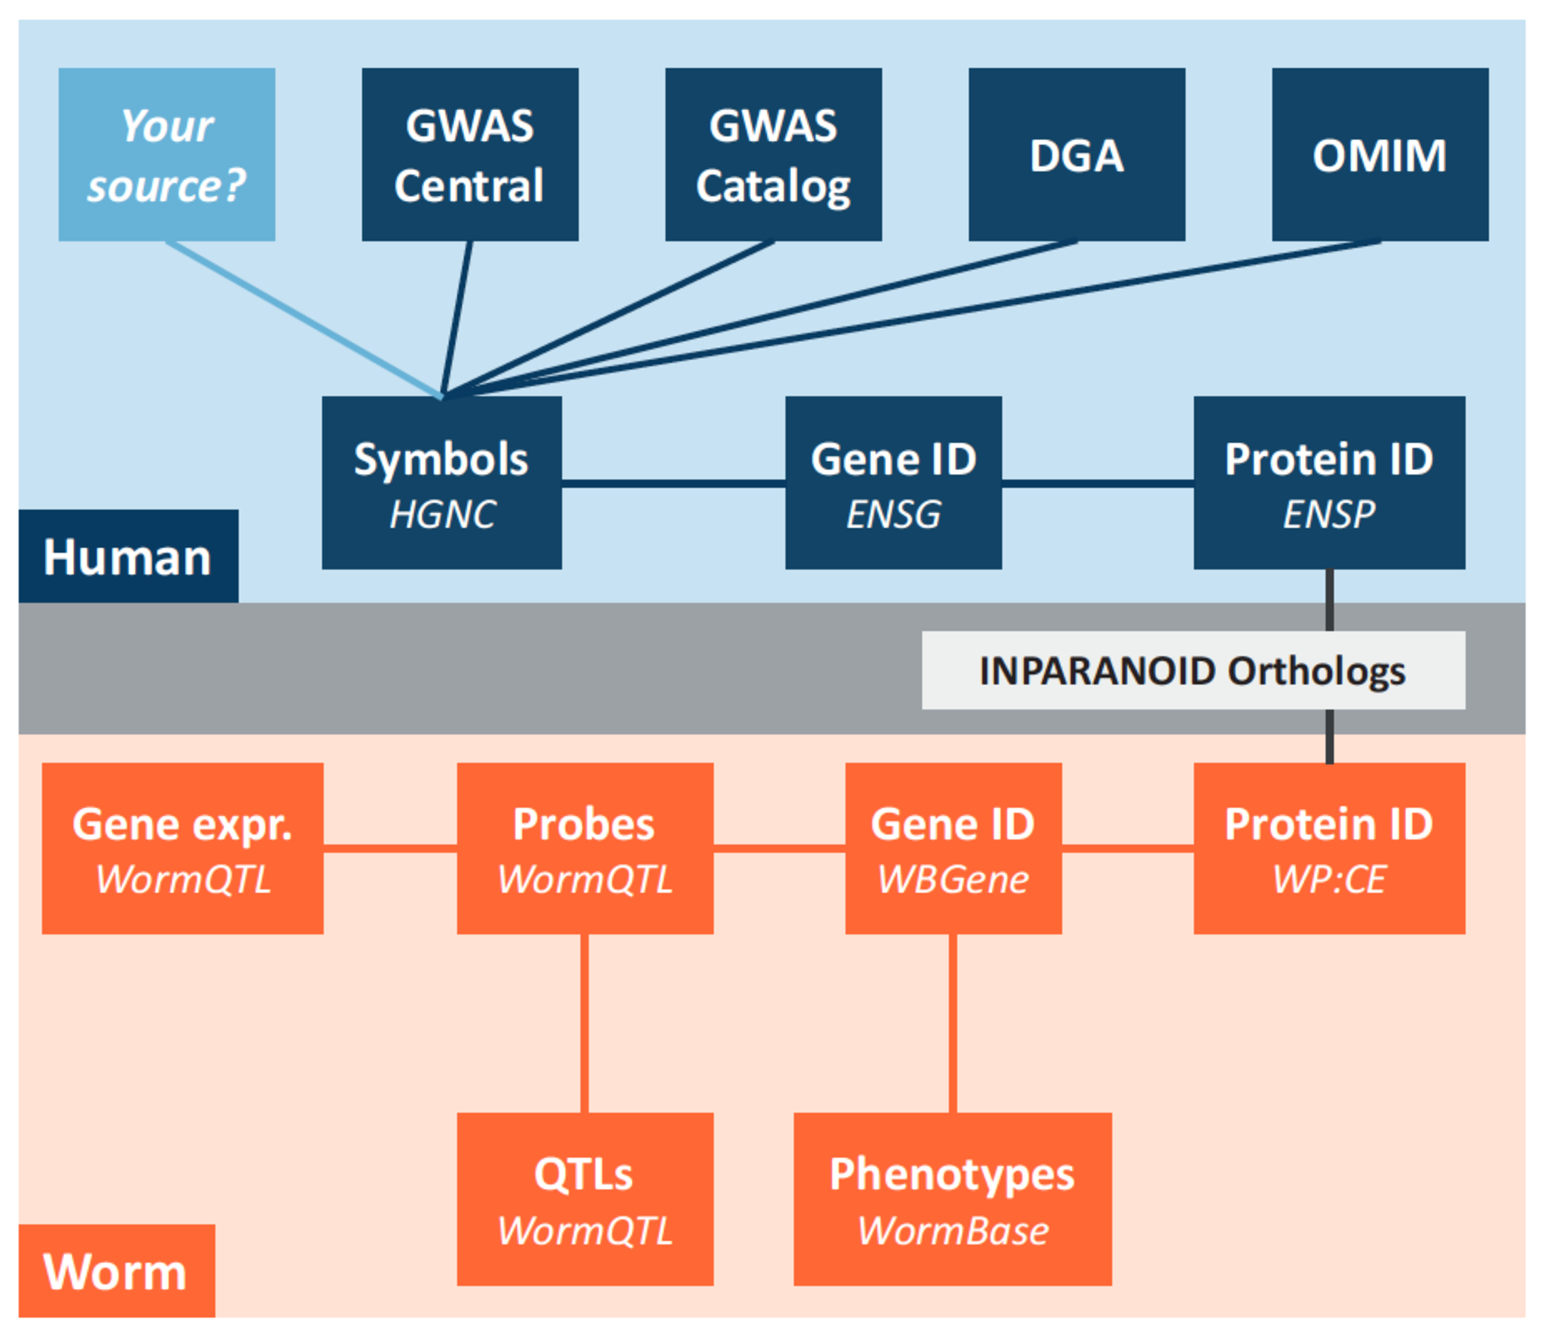
\includegraphics[scale=0.4]{img/wormqtl_mapping}
	\caption[Human and worm data integration]{Human and worm data integration. WormQTL\textsuperscript{HD} was compiled using data derived from WormQTL, WormBase, OMIM, DGA, GWAS Catalogue and GWAS Central.}
	\label{fig:wormqtl_mapping}
\end{figure}


\section{Implementation}
WormQTL\textsuperscript{HD} was compiled using data from six sources that are described below:
(I) WormQTL \cite{Snoek_2012}\footnote{The original paper erroneously cited \cite{Rodriguez_2013,Volkers_2013} here.}, (II) WormBase Phenotypes (\cite{Yook_2011}, (III) Online Mendelian Inheritance in Man (OMIM) \cite{Hamosh_2000}, (IV) The Disease and Gene Annotations (DGA) \cite{Peng_2012}, (V) NHGRI GWAS Catalogue \cite{Hindorff_2009} (\url{http://www.genome.gov/gwastudies}) and (VI) GWAS Central \cite{Thorisson_2009,Brookes_2000} (Figure \ref{fig:wormqtl_mapping}).
(I) WormQTL (\url{http://www.wormqtl.org}) contains many published ‘genetical genomics’ experiments and consists of 47 public data sets with eQTL data on 500 panels (Recombinant Inbred Lines or natural strains), 68,452 microarray probes, 1,630 samples and 1,579 markers.
The tools that were present in WormQTL, such as the QTL Finder and the Genome Browser, are also available in WormQTL\textsuperscript{HD}.
(II) WormBase is ‘an international consortium of biologists and computer scientists dedicated to providing the research community with accurate, current, accessible information concerning the genetics, genomics and biology of C. elegans and related nematodes’ (WormBase Mission statement, Todd Harris, 26 November 2012). From WormBase, we downloaded all the gene-phenotype associations (total 227,216) via WormMart.
(III) OMIM is one of the most popular databases containing 14,164 human gene-disease associations.
(IV) The DGA database (2,961 associations) was started in 2013 and claims to be more comprehensive than OMIM.
(V) The NHGRI GWAS Catalogue is a collection of 12,925 SNP-to-disease associations published in GWAS studies with at least 100,000 assayed SNPs and a \textsl{P}-value of $<$1.0 x 10\textsuperscript{-5}. The SNPs were linked to human genes by the authors of the original papers that have been included in the catalogue.
(VI) GWAS Central \cite{Thorisson_2009,Brookes_2000,Fredman_2002} is a database of summary level findings from genetic association studies.
The authors of GWAS Central gathered and curated many datasets from public domain projects, and supplied us with a list of 4,487 gene-disease associations having a \textsl{P}-value of $<$1.0 x 10\textsuperscript{-10}.
Because of the non-overlapping information in these four sources of human genes linked to disease, they are all provided and can be selected by the user.
Human and worm data are connected based on the detection of orthologous genes in these two species. We downloaded all INPARANOID orthologues between \textsl{C. elegans} and \textsl{Homo sapiens} with a 100\% bootstrap value.
The bootstrap value indicates how often the pair is found as reciprocally best matched in a sampling with a replacement procedure that was applied to the original Blast alignment.

To explore this database, WormQTL\textsuperscript{HD} features four major searching tools for different purposes. The starting points are summarized in Figure \ref{fig:wormqtl_overview} and described in detail below, followed by a short summary of the software used.


\begin{figure}
	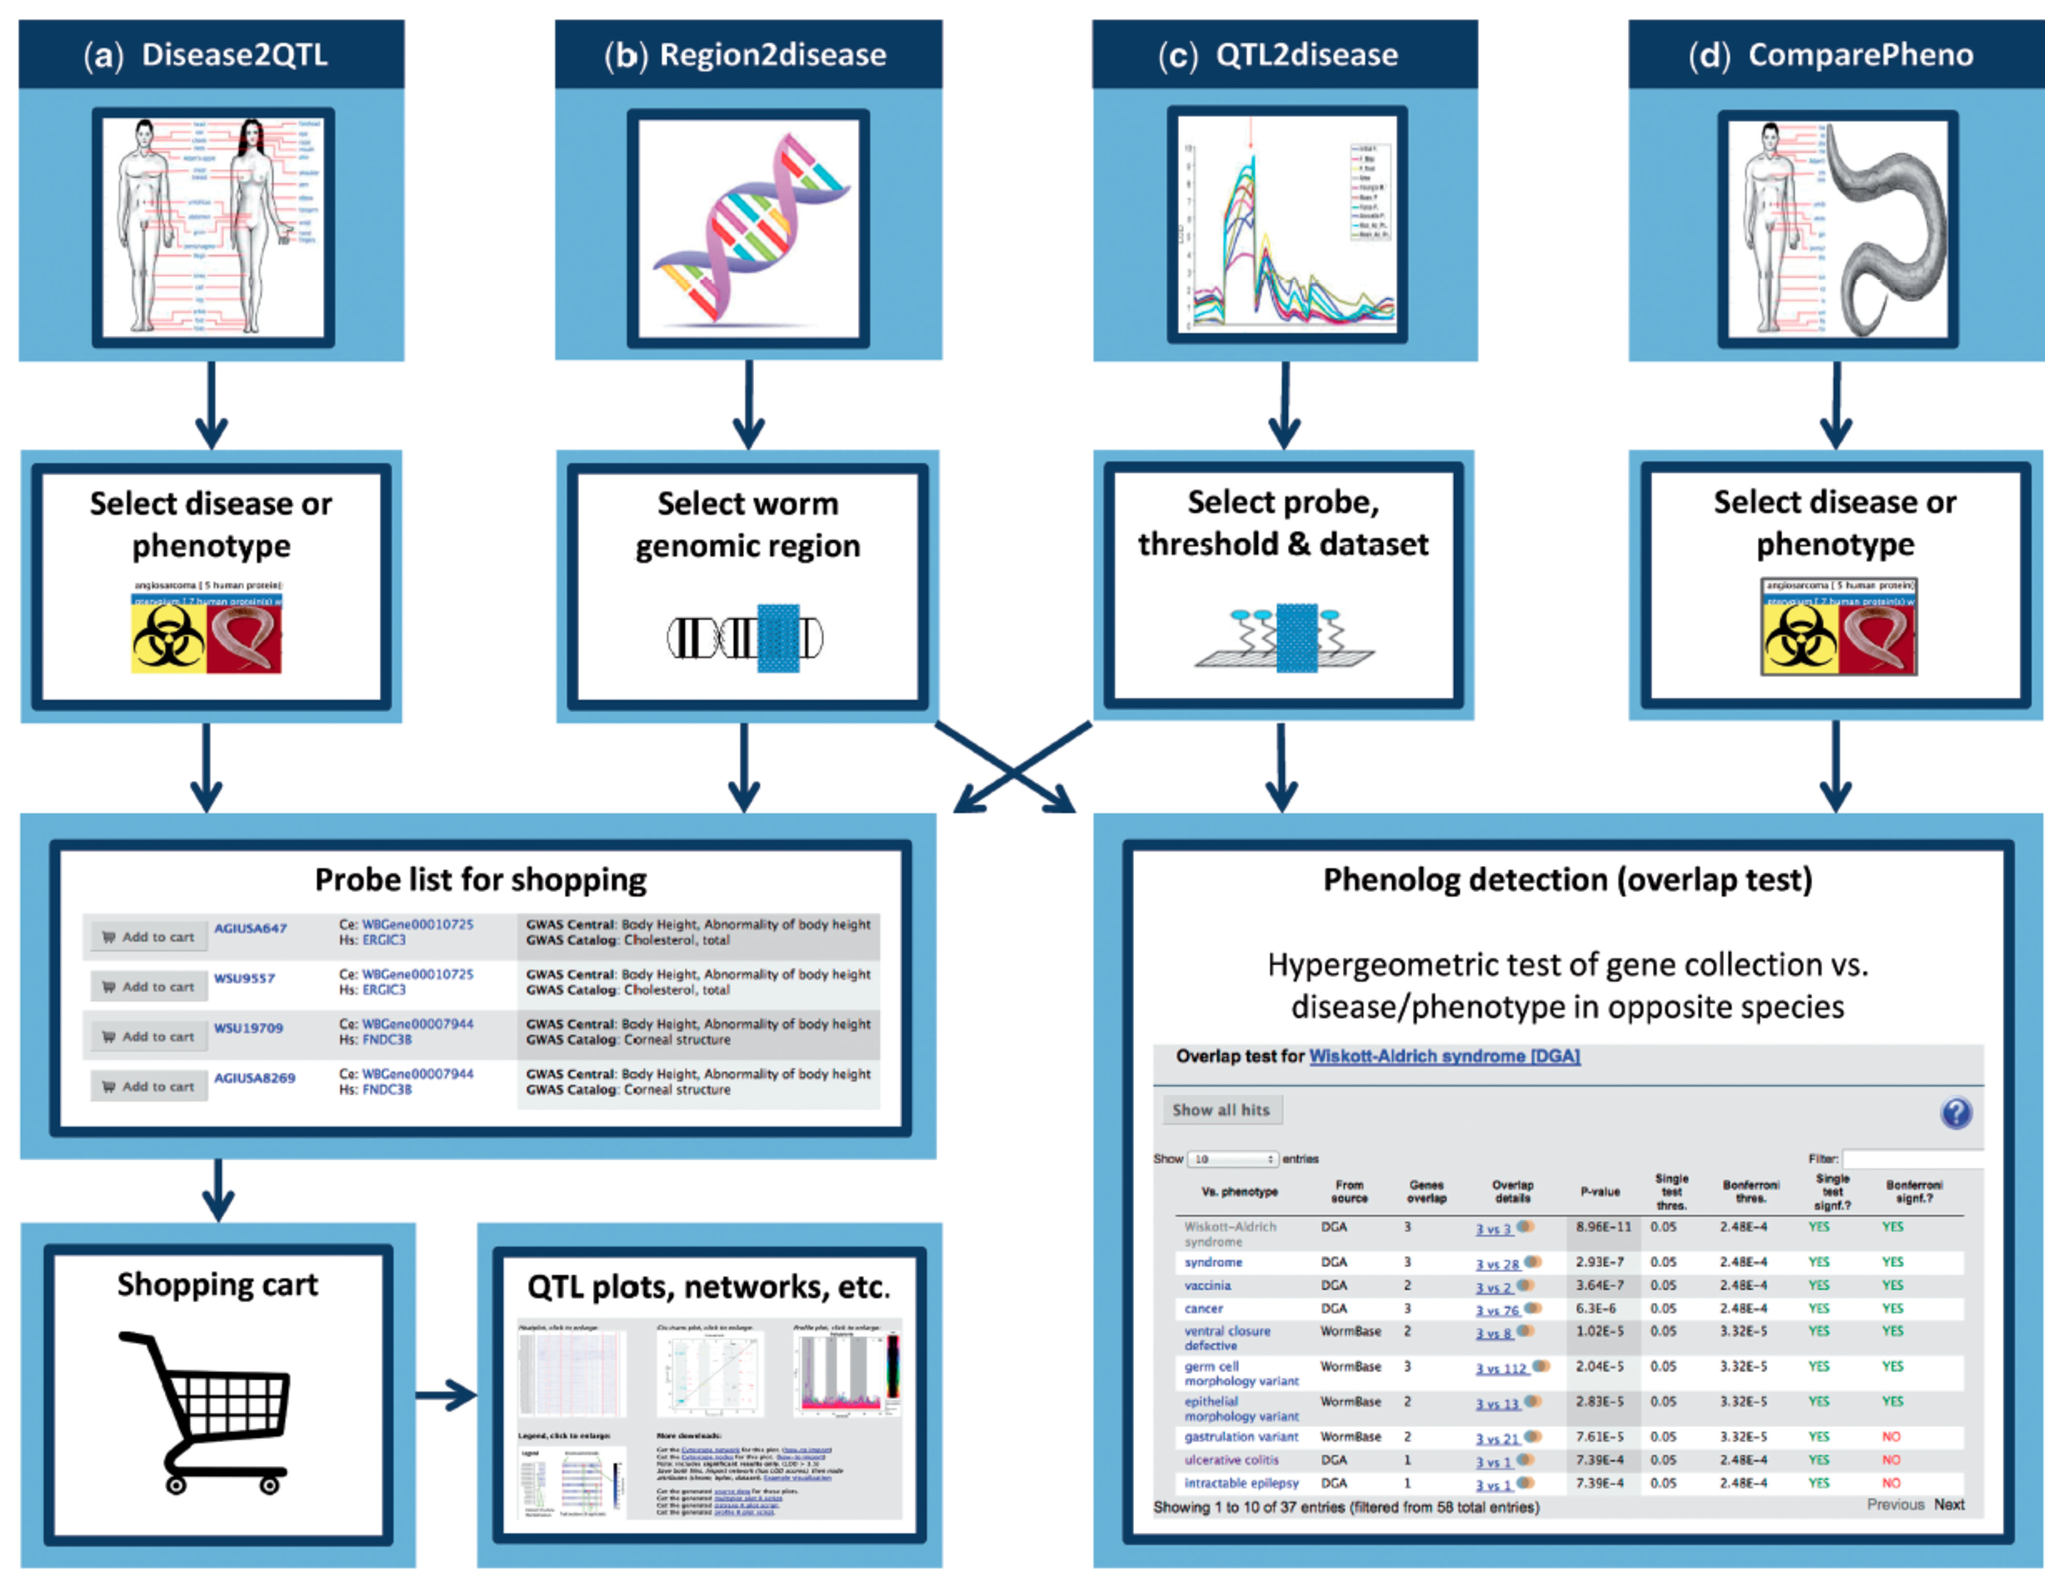
\includegraphics[width=1.0\linewidth]{img/wormqtl_overview}
	\caption[Cross-experiment search]{Cross-experiment search. WormQTL\textsuperscript{HD} provides four tools to explore the database: mapping human diseases to worm QTLs (Disease2QTL); mapping a worm genomic region to human diseases (Region2disease); mapping worm QTLs to human diseases (QTL2disease); and linking worm phenotypes to human diseases (ComparePheno).}
	\label{fig:wormqtl_overview}
\end{figure}


\subsection[Tool 1: ‘Disease2QTL’]{Tool 1: ‘Disease2QTL’, mapping human diseases to worm eQTLs}
Exploring the genetic variation data for human gene orthologues in worm can provide useful insight into the function and regulation of human diseases. WormQTL\textsuperscript{HD} provides a tool for human geneticists to explore novel causal genes for a specific human disease by using worm QTL findings.
Using a selection of one or multiple human diseases (from OMIM, DGA, NHGRI GWAS Catalogue or GWAS Central), a ‘shopping’ page is presented with worm gene expression probes and their human disease association.
More information about the gene orthology mapping and association studies can be browsed.
Users can put individual probes, or all probes at once, into the ‘shopping cart’.
Subsequently, they can explore the genetic variation of those genes across the different experiments and studies that are stored in the WormQTL\textsuperscript{HD} database.
The shopping cart is a central place in WormQTL\textsuperscript{HD} where users can see the various worm gene probes that they have selected, and create QTL/eQTL visualizations from the items in the shopping cart using ‘Plot QTLs’.

Using the ‘Plot QTLs’ function, researchers can test if genes associated with the selected diseases have any QTLs and if they map to a common genomic region.
Shared QTLs suggest that those genes are regulated by the same genetic variation and are possibly involved in the same biological pathways.
The genes with \textsl{cis}-QTLs in that genomic region are used as candidate genes in several types of studies \cite{Keurentjes_2007,Terpstra_2010,Snoek_2013}.
The same approach can be used for causal genes of human diseases.
Alternatively, users can also select worm phenotypes (1,504 total) instead of human diseases as a starting point. The shopping window is presented in exactly the same way as before, so users can browse human diseases from a worm phenotype perspective instead, or simply shop for probes of choice for a given worm phenotype and plot their QTLs, without considering any human disease relation.

\subsection[Tool 2: ‘Region2disease’]{Tool 2: ‘Region2disease’, mapping worm genomic regions to human diseases}
Researchers can link worm genomic regions to human diseases. This approach starts by selecting a region in the worm genome, e.g. a known ‘eQTL hotspot’, where a number of eQTLs are located.
The region is selected by providing the chromosome name, start and end base pair positions.
Users can quickly define a region of interest by using the location of any \textsl{C. elegans} gene.
The database then returns all worm gene expression probes that are annotated in this region.
From the probes, the corresponding worm genes are gathered, plus their human orthologues. The user is presented with a table containing the human-worm orthology and disease/phenotype associations in man and worm.
After shopping for some or all of the relevant probes, users can choose to visualize eQTL results for them (similar to Tool 1), or perform a disease enrichment test.

The hypergeometric gene overlap test \cite{Rivals_2006} to discover phenologs (phenotype orthologues) can be performed by clicking on ‘Disease enrichment’.
All probes in the region are linked to their corresponding genes in worm, and a test is performed whether this entire group of genes is significantly ‘enriched’ for one or more human diseases by overlapping orthologous groups and worm and human genes. The statistical significance of phenologs (\textsl{P}-value) is listed in an output table.
A significant result means that the input genomic region shares a significantly larger set of orthologous genes with a human disease than would be expected at random, even if the expressed phenotype in worm appears very different from the human disease phenotype (e.g. breast cancer and fertility).
This tool can provide novel interpretation of genomic regions of interest.

\subsection[Tool 3: ‘QTL2disease’]{Tool 3: ‘QTL2disease’, mapping worm QTLs to human diseases}
Researchers can start by selecting a QTL/eQTL in worm to find potential relationships with human diseases.
We can select QTLs of interest based on three criteria: a selected experiment, a certain threshold for significance (LOD score) and a specific gene expression probe with a suspected QTL.
If there is a QTL with a LOD score above the threshold, we automatically select the closest 50 probes on both sides of the highest peak marker.
These probes are presented and available for browsing, shopping and plotting of QTLs, or can be the input for the disease enrichment test to find phenologs.

\subsection[Tool 4: ‘ComparePheno’]{Tool 4: ‘ComparePheno’, linking worm phenotypes to human diseases}
WormQTL\textsuperscript{HD} also provides a tool that links human diseases to classical worm phenotypes (and \textsl{vice versa}) to discover phenologs in a systematic way.
Users begin by selecting one or more human diseases and clicking on ‘Compare’.
The genes associated with the selected disease are tested for enrichment against all sets of known associated genes for worm phenotypes. The result reveals functionally coherent, evolutionarily conserved gene networks.

Alternatively, users can also start by selecting worm phenotypes, which are tested against human diseases. In addition to cross-species testing, results of within-species disease enrichment are also available (e.g. to find the closest related human disease for another input human disease).

\subsection{Software used}
All the software has been implemented using the open source ‘MOLecular GENetics Information Systems’— MOLGENIS—toolkit \cite{Swertz_2010a}.
The MOLGENIS toolkit is Java-based software to generate tailored research infrastructure on-demand \cite{Swertz_2007}.
In particular, we built on an existing MOLGENIS application, the extensible xQTL workbench \cite{Arends_2012} and the R/qtl QTL mapping and visualization package for the R language \cite{Broman_2003,Arends_2010}.
All software is available as open source on \url{http://github.com/molgenis} for others to reuse locally.
Related technical documentation is available at \url{http://www.molgenis.org/xqtl}\footnote{The URL in the original paper is no longer active and was updated here.}, \url{http://www.rqtl.org} and \url{http://www.molgenis.org}.



\section{Results}
To demonstrate the added value of WormQTL\textsuperscript{HD}, we have reproduced findings from known studies and have shown that novel insights and hypotheses can be achieved with little time and effort.
Subsequently, we performed a broad-sweep disease-enrichment test to find all non-evident phenologs and to explore which new putative candidate genes for human diseases could be elucidated for future research.

\subsection[Case 1: McGary \textsl{et al.}]{Case 1: Linking disease to worm phenotype from McGary \textsl{et al.} \cite{McGary_2010}}
McGary \textsl{et al.} performed a phenolog mapping between the high incidence of male \textsl{C. elegans} progeny to human breast/ovarian cancers. Of 4,649 total orthologues, McGary \textsl{et al.} reported 3 overlapping genes of 12 human disease-associated genes and 16 worm phenotype-associated genes—which is a significant enrichment (hypergeometric test \textsl{P}-value of $\leq$ 7.2 x 10\textsuperscript{-6}).
From the 13 worm phenotype-associated genes that were not overlapping, 9 had orthologues that had already been linked to breast cancer in the primary literature.
They implicated the remaining four genes as new breast cancer candidates. We replicated these findings using the ComparePheno tool of WormQTL\textsuperscript{HD}, searching for the WormBase phenotype ‘high incidence male progeny’.
The first human disease among the results is ‘\{Breast cancer, susceptibility to\}, 114480 (3)’ from OMIM. Our tool reported 2 overlapping genes of 4 human disease-associated genes and 63 genes from the worm phenotype.
This resulted in a \textsl{P}-value $\leq$ 1.4 x 10\textsuperscript{-3} (uncorrected). The second best human hit in the results is ‘malignant neoplasm of ovary’ from DGA.
We found two overlapping genes of six ovarian cancer associated genes, resulting in a \textsl{P}-value $\leq$ 3.41 x 10\textsuperscript{-3} (uncorrected).
ComparePheno also indicated enrichment of these categories.
The \textsl{P}-values are ‘less significant’ than McGary et al. because (i) their definition of ‘high incidence male progeny’ included only 16 rather than 63 genes and (ii) they used an older INPARANOID version, so the overlap test was performed on a different orthologue mapping.
Together, these results from our  database do indeed replicate their findings.
See Online Use Case 1 on the Help page to repeat this case.

\subsection[Case 2: Li \textsl{et al.}]{Case 2: Worm eQTL hotspot from two temperature expression data from Li \textsl{et al.} \cite{Li_2006}}
Li \textsl{et al.} \cite{Li_2006} found an eQTL hotspot (77.56Mb on chromosome V) on the worm genome in which genetic variation is associated with the expression of 66 genes, while these genes are located elsewhere on the genome.
This indicates that these genes are possibly involved in the same biological process/pathway and potentially share a regulatory element.
They may be physically located on the eQTL hotspot, which controls gene expression responding to different ambient temperatures.
First, we used the Region2disease tool and input positions ChrV:15430739-16430739 (a non-cumulative 1 Mb region around the hotspot).
We put all 931 probes located in this region in the shopping cart, and selected ‘Disease enrichment’.
The best hit was ‘Response to antineoplastic agents’ (agents used in chemotherapeutic treatment of cancer) from GWAS Catalogue (\textsl{P}-value $\leq$ 4.92 x 10\textsuperscript{-3}, uncorrected).
For this hit, the associated human gene, \textsl{PPP2R5E}, is orthologous to WBGene00012348 (\textsl{pptr-1}) present in this region. The best WormBase hit is ‘thermotolerance increased’ (\textsl{P}-value $\leq$ 1.5 x 10\textsuperscript{-2}, uncorrected), also via association with \textsl{pptr-1}.
Padmanabhan \textsl{et al.} \cite{Padmanabhan_2009} showed that \textsl{pptr-1} is involved in regulating subcellular localization and transcriptional activity of the forkhead transcription factor \textsl{daf-16}.
Rodriguez \textsl{et al.} \cite{Rodriguez_2013} reviewed the role of heat stress response experiments in \textsl{C. elegans} for detecting human disease genes.
They reported that \textsl{daf-16} in worms controls lifespan and stress response.
In humans, the \textsl{daf-16} orthologue \textsl{FOXO3A} is associated with aging and prevalence of cancer \cite{Willcox_2008}.
Using the Disease2QTL tool, a search for ‘Response to antineoplastic agents’ results in six probes for orthologues of \textsl{PPP2R5E} (WBGene00012348) and \textsl{ACOX3} (WBGene00019060).
We selected them all and plotted the QTLs.
This revealed a highly significant (LOD $>$ 50) \textsl{cis}-eQTL for \textsl{pptr-1} in the Rockman \textsl{et al.} \cite{Rockman_2010} dataset.
Given all the evidence, we believe \textsl{pptr-1} might be an interesting candidate in the further development of a temperature-based \textsl{C. elegans} model for understanding human cancer and developing potential therapeutic drugs.
Moreover, it shows that combining the ‘Region2disease’ and ‘Disease2QTL’ tools can lead to an interesting hypothesis ready for experimental validation.
See Online Use Case 2 on the Help page to reproduce this case.

\subsection[Case 3: Rodriguez \textsl{et al.}]{Case 3: Osmotic stress as a model for Bar\-det-\-Biedl syndrome from Rodriguez \textsl{et al.} \cite{Rodriguez_2013}}
Rodriguez \textsl{et al.} proposed hypertonic or osmotic stress in \textsl{C. elegans} as a model to study human diseases related to protein aggregation, such as Alzheimer’s and Parkinson’s.
Hypertonic stress due to loss of water causes an intracellular ionic imbalance, which leads to rapid accumulation of organic osmotic glycerol and accumulation of damaged proteins.
Shaye and Greenwald \cite{Shaye_2011} showed that \textsl{osm-12} (associated with osmotic stress response) is orthologous to \textsl{BBS7} in man, which is associated to Bardet-Biedl syndrome \cite{Badano_2003}.
We used the Disease2QTL tool to look for QTLs associated with Bardet-Biedl syndrome by selecting all ‘Bardet-Biedl syndrome’ entries (seven in total) from OMIM.
When we plotted the QTLs in worm for these entries, three significant eQTLs (LOD $>$ 5) were found for \textsl{osm-12} (in \textsl{cis}), \textsl{bbs-5} (also in \textsl{cis}) and \textsl{bbs-2} (in \textsl{trans}).
The strongest QTL (LOD $>$ 6) was found for \textsl{bbs-5}, reported by probe AGIUSA3442 in the Rockman \textsl{et al.} dataset.
We used the QTL2disease tool to investigate this QTL further. It revealed a nearby, very significant eQTL (LOD $>$ 10) for a gene named \textsl{T07C4.10}, which can be investigated further as a potential candidate for this disease model.
See Online Use Case 3 on the Help page to replicate this example.

\subsection[Novel disease-gene associations]{Novel disease-gene associations by ‘broad-sweep’ disease-enrichment test}
We performed hypergeometric gene overlap tests to find phenologs between all worm phenotypes versus all human diseases.
Table \ref{table:wormqtl_enrichment} lists the 15 most significant hits for human diseases that have significant gene overlap with worm phenotypes (see Tables \ref{table:wormqtl_enrichment_suppl1} and \ref{table:wormqtl_enrichment_suppl2} for the top 100).
New candidate genes for human diseases can be discovered from phenologs by investigating human orthologues of worm genes that did not overlap with known human genes of the disease of interest.

McGary \textsl{et al.} \cite{McGary_2010} reported ‘Zellweger syndrome’ in man to be a phenolog with ‘Reduced number of peroxisomes’ in yeast (\textsl{P}-value $<$ 1.0 x 10\textsuperscript{-9}).
Our best hit was ‘Zellweger syndrome’ with ‘peroxisome physiology variant’ in worm (\textsl{P}-value $<$ 3.6 x 10\textsuperscript{-10}).
Encouragingly, certain top hits such as ‘coenzyme Q depleted’ in worm versus ‘Coenzyme Q10 deficiency’ in man, and ‘spontaneous mutation rate increased’ in worm versus ‘Mismatch repair cancer syndrome’ in man make sense, thereby validating this approach and adding credibility to potentially non-evident human disease models.

\begin{sidewaystable}
\footnotesize
\begin{tabulary}{\linewidth}{LLRRRL}
  Phenotype\textsubscript{1} (Ce) & Phenotype\textsubscript{2} (Hs) & \textsl{n}\textsubscript{1} & \textsl{n}\textsubscript{2} & \textsl{k} & \mbox{\textsl{P}-value~~~~~~} \\
  \hline
  Peroxisome physiology variant & Zellweger syndrome, 214100 (3) [OMIM] & 3 & 4 & 3 & 3.58E-10 \\
  Coenzyme Q depleted & Coenzyme Q10 deficiency, 607426 (3) [OMIM] & 9 & 3 & 3 & 7.53E-09 \\
  Spontaneous mutation rate increased & Mismatch repair cancer syndrome, 276300 (3) [OMIM] & 42 & 4 & 4 & 9.88E-09 \\
  Mitochondrial metabolism variant & Coenzyme Q10 deficiency, 607426 (3) [OMIM] & 17 & 3 & 3 & 6.09E-08 \\
  AWA odorant chemotaxis defective & Cardiofaciocutaneous syndrome, 115150 (3) [OMIM] & 3 & 2 & 2 & 3.64E-07 \\
  Peroxisome physiology variant & Adrenoleukodystrophy, neonatal, 202370 (3) [OMIM] & 3 & 3 & 2 & 1.09E-06 \\
  AWC odorant chemotaxis defective & Cardiofaciocutaneous syndrome, 115150 (3) [OMIM] & 5 & 2 & 2 & 1.21E-06 \\
  Germ nuclei rachis & Cardiofaciocutaneous syndrome, 115150 (3) [OMIM] & 6 & 2 & 2 & 1.82E-06 \\
  Excretory cell development variant & Rheumatoid arthritis [GWAS Catalogue] & 3 & 5 & 2 & 3.64E-06 \\
  Bacterially unswollen & Cardiofaciocutaneous syndrome, 115150 (3) [OMIM] & 11 & 2 & 2 & 6.67E-06 \\
  Organism starvation response variant & Ovarian cancer, somatic, 604370 (3) [OMIM] & 12 & 2 & 2 & 8.00E-06 \\
  Neuron development variant & Diastolic blood pressure [GWAS Catalog] & 17 & 11 & 3 & 9.85E-06 \\
  Ventral closure defective & Wiskott-Aldrich syndrome [DGA] & 8 & 3 & 2 & 1.02E-05 \\
  Egg laying imipramine resistant & Bone mineral density [GWAS Catalog] & 26 & 23 & 4 & 1.08E-05 \\
  mRNA export variant & disease by infectious agent [DGA] & 4 & 6 & 2 & 1.09E-05 \\
  \hline
\end{tabulary}
\caption[Top 15 results for the disease enrichment]{Top 15 results for the ‘broad-sweep’ disease enrichment. \textsl{n}\textsubscript{1} indicates the number of orthologues in \textsl{C. elegans} (Ce) with phenotype\textsubscript{1}, \textsl{n}\textsubscript{2} the number in \textsl{H. sapiens} (Hs) with phenotype\textsubscript{2} and k the number in both sets. The significance of each phenolog is assessed by the hypergeometric probability (\textsl{P}-value).}
\label{table:wormqtl_enrichment}
\end{sidewaystable}

\linespread{1.00} % need to squeeze a bit to fit these tables nicely

\begin{table}
\tiny
\begin{tabulary}{\linewidth}{LLRRRL}
  Phenotype\textsubscript{1} (Ce) & Phenotype\textsubscript{2} (Hs) & \textsl{n}\textsubscript{1} & \textsl{n}\textsubscript{2} & \textsl{k} & \mbox{\textsl{P}-value~~~~~~} \\
  \hline
  constipated & Cardiofaciocutaneous syndrome, 115150 (3) [OMIM] & 14 & 2 & 2 & 1.10E-05 \\
  neuron development variant & Blood Pressure [GWAS Central] & 17 & 12 & 3 & 1.31E-05 \\
  reproductive system development variant & Palmitoleic acid (16:1n-7) plasma levels [GWAS Catalog] & 6 & 5 & 2 & 1.82E-05 \\
  germ cell morphology variant & Wiskott-Aldrich syndrome [DGA] & 112 & 3 & 3 & 2.04E-05 \\
  life span variant & Coenzyme Q10 deficiency, 607426 (3) [OMIM] & 114 & 3 & 3 & 2.15E-05 \\
  organism starvation response variant & Colorectal cancer, somatic, 114500 (3) [OMIM] & 12 & 3 & 2 & 2.40E-05 \\
  gastrulation variant & vaccinia [DGA] & 21 & 2 & 2 & 2.55E-05 \\
  neuron development variant & Blood pressure [GWAS Catalog] & 17 & 15 & 3 & 2.69E-05 \\
  epithelial morphology variant & Wiskott-Aldrich syndrome [DGA] & 13 & 3 & 2 & 2.83E-05 \\
  osmotic stress response variant & Chronic obstructive pulmonary disease [GWAS Catalog] & 13 & 3 & 2 & 2.83E-05 \\
  radiation induced reproductive cell death variant & Mismatch repair cancer syndrome, 276300 (3) [OMIM] & 10 & 4 & 2 & 3.26E-05 \\
  distal tip cell development variant & Pulmonary function (interaction) [GWAS Catalog] & 6 & 7 & 2 & 3.81E-05 \\
  dauer arrest variant & Ovarian cancer, somatic, 604370 (3) [OMIM] & 26 & 2 & 2 & 3.94E-05 \\
  bag of worms & Heart Rate [GWAS Central] & 29 & 2 & 2 & 4.92E-05 \\
  halothane hypersensitive & Leigh syndrome, 256000 (3) [OMIM] & 6 & 8 & 2 & 5.07E-05 \\
  vulvaless & Cardiofaciocutaneous syndrome, 115150 (3) [OMIM] & 30 & 2 & 2 & 5.27E-05 \\
  transgene expression variant & Pulmonary function (interaction) [GWAS Catalog] & 147 & 7 & 4 & 5.30E-05 \\
  sodium chloride chemotaxis defective & Cardiofaciocutaneous syndrome, 115150 (3) [OMIM] & 31 & 2 & 2 & 5.64E-05 \\
  synaptogenesis variant & Hippocampal atrophy [GWAS Catalog] & 13 & 4 & 2 & 5.65E-05 \\
  body size variant & Inflammatory bowel disease [GWAS Catalog] & 11 & 30 & 3 & 5.77E-05 \\
  gastrulation variant & Wiskott-Aldrich syndrome [DGA] & 21 & 3 & 2 & 7.61E-05 \\
  pathogen susceptibility increased & Cardiofaciocutaneous syndrome, 115150 (3) [OMIM] & 36 & 2 & 2 & 7.64E-05 \\
  level of protein expression variant & hepatitis B [DGA] & 39 & 2 & 2 & 8.98E-05 \\
  male gonad morphology variant & Bone mineral density [GWAS Catalog] & 3 & 23 & 2 & 9.17E-05 \\
  flaccid & Electrocardiographic traits [GWAS Catalog] & 13 & 5 & 2 & 9.41E-05 \\
  paraquat resistant & Ovarian cancer, somatic, 604370 (3) [OMIM] & 41 & 2 & 2 & 9.94E-05 \\
  reproductive system development variant & Metabolic traits [GWAS Catalog] & 6 & 11 & 2 & 9.94E-05 \\
  spontaneous mutation rate increased & Muir-Torre syndrome, 158320 (3) [OMIM] & 42 & 2 & 2 & 1.04E-04 \\
  dauer formation variant & Ovarian cancer, somatic, 604370 (3) [OMIM] & 43 & 2 & 2 & 1.09E-04 \\
  dauer arrest variant & Colorectal cancer, somatic, 114500 (3) [OMIM] & 26 & 3 & 2 & 1.18E-04 \\
  loss of asymmetry ASE & Cardiofaciocutaneous syndrome, 115150 (3) [OMIM] & 47 & 2 & 2 & 1.31E-04 \\
  large cytoplasmic granules early emb & Eye Color [GWAS Central] & 28 & 3 & 2 & 1.37E-04 \\
  gonad sheath contraction rate reduced & Systolic blood pressure [GWAS Catalog] & 7 & 11 & 2 & 1.39E-04 \\
  osmotic stress response variant & Sudden cardiac arrest [GWAS Catalog] & 13 & 6 & 2 & 1.41E-04 \\
  male tail morphology variant & substance dependence [DGA] & 29 & 3 & 2 & 1.47E-04 \\
  dauer constitutive & Ovarian cancer, somatic, 604370 (3) [OMIM] & 50 & 2 & 2 & 1.49E-04 \\  
  excessive blebbing early emb & Eye Color [GWAS Central] & 30 & 3 & 2 & 1.57E-04 \\
  nucleus reforms cell division remnant early emb & lymphoma [DGA] & 14 & 6 & 2 & 1.64E-04 \\
  egg laying variant & Body mass index (interaction) [GWAS Catalog] & 228 & 3 & 3 & 1.75E-04 \\
  cell polarity reversed & Bone mineral density [GWAS Catalog] & 4 & 23 & 2 & 1.83E-04 \\
  nuclear positioning variant & hepatitis [DGA] & 18 & 5 & 2 & 1.84E-04 \\
  alae variant & Immune reponse to smallpox (secreted IFN-alpha) [GWAS Catalog] & 11 & 8 & 2 & 1.85E-04 \\
  habituation variant & Asthma [GWAS Catalog] & 15 & 6 & 2 & 1.89E-04 \\
  \hline
\end{tabulary}
\caption[Result hits 16-58 for the disease enrichment]{Result hits 16-58 for the ‘broad-sweep’ disease enrichment. \textsl{n}\textsubscript{1} indicates the number of orthologues in \textsl{C. elegans} (Ce) with phenotype\textsubscript{1}, \textsl{n}\textsubscript{2} the number in \textsl{H. sapiens} (Hs) with phenotype\textsubscript{2} and k the number in both sets. The significance of each phenolog is assessed by the hypergeometric probability (\textsl{P}-value).}
\label{table:wormqtl_enrichment_suppl1}
\end{table}

\begin{table}
\tiny
\begin{tabulary}{\linewidth}{LLRRRL}
  Phenotype\textsubscript{1} (Ce) & Phenotype\textsubscript{2} (Hs) & \textsl{n}\textsubscript{1} & \textsl{n}\textsubscript{2} & \textsl{k} & \mbox{\textsl{P}-value~~~~~~~} \\
  \hline
  age associated fluorescence increased & narcolepsy [DGA] & 57 & 2 & 2 & 1.94E-04 \\
  pharyngeal development variant & PR interval [GWAS Catalog] & 24 & 4 & 2 & 1.99E-04 \\
  movement variant & Acute lymphoblastic leukemia (childhood) [GWAS Catalog] & 19 & 5 & 2 & 2.06E-04 \\
  miRNA expression variant & Type 2 diabetes [GWAS Catalog] & 50 & 25 & 4 & 2.12E-04 \\
  hypoxia hypersensitive & Mismatch repair cancer syndrome, 276300 (3) [OMIM] & 25 & 4 & 2 & 2.17E-04 \\
  P0 spindle rotation failure early emb & Colitis, Ulcerative [GWAS Central] & 9 & 11 & 2 & 2.38E-04 \\
  paralyzed body & Dyssegmental dysplasia, Silverman-Handmaker type, 224410 (3) [OMIM] & 1 & 1 & 1 & 2.46E-04 \\
  protein phosphorylation increased & glioma [DGA] & 21 & 5 & 2 & 2.52E-04 \\
  transgene expression variant & Red blood cell traits [GWAS Catalog] & 147 & 17 & 5 & 2.52E-04 \\
  anaphase bridging & lymphoma [DGA] & 18 & 6 & 2 & 2.75E-04 \\
  body wall muscle morphology variant & Response to antidepressant treatment [GWAS Catalog] & 22 & 5 & 2 & 2.77E-04 \\
  coelomocyte uptake defective & Peters anomaly, 604229 (3) [OMIM] & 70 & 2 & 2 & 2.93E-04 \\
  paraquat resistant & Colorectal cancer, somatic, 114500 (3) [OMIM] & 41 & 3 & 2 & 2.96E-04 \\
  HSN migration variant & Bone mineral density [GWAS Catalog] & 24 & 23 & 3 & 2.97E-04 \\
  small & Leukoencephalopathy with vanishing white matter, 603896 (3) [OMIM] & 174 & 4 & 3 & 2.99E-04 \\
  embryo osmotic integrity defective early emb & Cardiofaciocutaneous syndrome, 115150 (3) [OMIM] & 71 & 2 & 2 & 3.01E-04 \\
  endomitotic oocytes & glioma [DGA] & 23 & 5 & 2 & 3.04E-04 \\
  egg laying defective & Bone mineral density [GWAS Catalog] & 174 & 23 & 6 & 3.11E-04 \\
  dauer formation variant & Colorectal cancer, somatic, 114500 (3) [OMIM] & 43 & 3 & 2 & 3.26E-04 \\
  P0 spindle rotation delayed early emb & Platelet counts [GWAS Catalog] & 6 & 20 & 2 & 3.41E-04 \\
  drug induced gene expression variant & Ventricular conduction [GWAS Catalog] & 10 & 12 & 2 & 3.55E-04 \\
  multiple nuclei oocyte & Cholesterol [GWAS Central] & 45 & 3 & 2 & 3.58E-04 \\
  extended life span & Leigh syndrome, 256000 (3) [OMIM] & 206 & 8 & 4 & 3.83E-04 \\
  short & Palmitoleic acid (16:1n-7) plasma levels [GWAS Catalog] & 26 & 5 & 2 & 3.89E-04 \\
  lipid composition variant & Urate levels [GWAS Catalog] & 9 & 14 & 2 & 3.92E-04 \\
  fat content increased & Ovarian cancer, somatic, 604370 (3) [OMIM] & 81 & 2 & 2 & 3.93E-04 \\
  fewer germ cells & Mean corpuscular hemoglobin [GWAS Catalog] & 34 & 4 & 2 & 4.04E-04 \\
  oogenesis variant & rheumatoid arthritis [DGA] & 83 & 2 & 2 & 4.13E-04 \\
  oocyte number decreased & Cholesterol, LDL [GWAS Central] & 194 & 4 & 3 & 4.14E-04 \\
  germ cell compartment anucleate & Cardiofaciocutaneous syndrome, 115150 (3) [OMIM] & 84 & 2 & 2 & 4.23E-04 \\
  early larval lethal & kidney disease [DGA] & 85 & 2 & 2 & 4.33E-04 \\
  dauer constitutive & Colorectal cancer, somatic, 114500 (3) [OMIM] & 50 & 3 & 2 & 4.42E-04 \\
  transgene expression variant & Systolic blood pressure [GWAS Catalog] & 147 & 11 & 4 & 4.46E-04 \\
  sex determination variant & Bone mineral density [GWAS Catalog] & 6 & 23 & 2 & 4.54E-04 \\
  body wall muscle thick filament variant & Atrial septal defect 3 (3) [OMIM] & 2 & 1 & 1 & 4.92E-04 \\
  response to injury variant & Ulcerative colitis [GWAS Catalog] & 6 & 24 & 2 & 4.95E-04 \\
  diplotene progression during oogenesis variant & Response to Vitamin E supplementation [GWAS Catalog] & 38 & 4 & 2 & 5.05E-04 \\
  osmotic stress response variant & Systolic blood pressure [GWAS Catalog] & 13 & 11 & 2 & 5.12E-04 \\
  male tail morphology variant & Bone mineral density [GWAS Catalog] & 29 & 23 & 3 & 5.27E-04 \\
  anchor cell invasion variant & Attention deficit hyperactivity disorder [GWAS Catalog] & 57 & 12 & 3 & 5.27E-04 \\
  exploded through vulva & Bone mineral density [GWAS Catalog] & 277 & 23 & 7 & 6.03E-04 \\
  antimicrobial gene expression variant & Ventricular conduction [GWAS Catalog] & 13 & 12 & 2 & 6.13E-04 \\
  \hline
\end{tabulary}
\caption[Result hits 59-100 for the disease enrichment]{Result hits 59-100 for the ‘broad-sweep’ disease enrichment. \textsl{n}\textsubscript{1} indicates the number of orthologues in \textsl{C. elegans} (Ce) with phenotype\textsubscript{1}, \textsl{n}\textsubscript{2} the number in \textsl{H. sapiens} (Hs) with phenotype\textsubscript{2} and k the number in both sets. The significance of each phenolog is assessed by the hypergeometric probability (\textsl{P}-value).}
\label{table:wormqtl_enrichment_suppl2}
\end{table}

\linespread{1.05} % and back to normal

\section{Discussion}
The current version of WormQTL\textsuperscript{HD} (August 2013) is a comprehensive and compendious database that enables molecular model organism data to be studied in the context of human diseases.
Just as with WormQTL \cite{Snoek_2012}\footnote{The original paper erroneously cited \cite{Rodriguez_2013} here.}, we believe that WormQTL\textsuperscript{HD} will be continuously curated by the members of the \textsl{C. elegans} community.
The results of the ‘broad-sweep’ disease-enrichment test in combination with the web tool will be of special interest to researchers in the human or worm domain.
We believe these results could also be applied to prioritize the pathogenic variants increasingly being produced by next-generation sequencing in diagnostic labs.
Genetic variants affecting human genes of unknown function may have worm orthologues that are part of human-worm phenologs and these may reveal or imply a role in a human disease.
Thus, through functionally conserved networks, missing information can be inferred and candidate genes can be selected via model organisms.

The approach of WormQTL\textsuperscript{HD} is conceptually similar to that described by Smedley \textsl{et al.} \cite{Smedley_2013}.
They created an automated method called PhenoDigm to provide evidence about gene-disease associations by analysing phenotypic information. In their case, phenotypes consist of a collection of ontology terms, which are aligned and scored to derive an overall phenotype-similarity score.
Using this method, known gene-phenotype associations in model organisms (mouse, zebrafish) can be transferred to other organisms such as man, and help us to understand the genetic cause of disease.
This method works best when the model organism is physiologically close to man and has comparable classical phenotypes. It would therefore be less useful for \textsl{C. elegans}.
However, combining the molecular (WormQTL\textsuperscript{HD}) and phenotypical (PhenoDigm) approaches may result in a very powerful tool to discover novel gene-disease associations in man, especially when using physiologically close model organisms.

We plan to further develop the WormQTL\textsuperscript{HD} data and toolset.
There might be more ways in which researchers would like to search through the large amounts of data, for example, based on custom lists of gene identifiers, or by combining tools such as finding QTLs within specific regions.
The QTL plots could be improved or replaced with interactive graphs that are more informative and would allow the users to continue ‘drilling down’ in the data instead of returning to the home page for a new analysis with a different tool.
Furthermore, we envisage close integration with other data sources and tools such as WormNet, R/qtl and GO Enrichment to provide even more biological context and analytical tools for the user.

Our new database makes this data attractive and easy-to-use for an even wider community of quantitative geneticists working on worms and man.
We are committed to maintaining the data and software in the future and invite the community to add and share their new data and ideas.

\section*{Supplementary Data}
Supplementary Data are available at NAR Online.

\section*{Acknowledgements}
We thank Prof. Anthony J. Brookes and Dr Robert Hastings at the Department of Genetics, University of Leicester, UK, for providing us with the data from GWAS Central via a custom batch query, WormBase, the McKusick-Nathans Institute of Genetic Medicine (OMIM), Northwestern University, Chicago, Illinois (DGA) and The National Human Genome Research Institute (GWAS CATALOG) for openly providing their data in a structured way. We also thank Bart Charbon, Erwin Winder and Dennis Hendriksen for proofreading the manuscript and for their helpful suggestions, Jackie Senior for editing, Patrick Deelen, Roan Kanninga and Pieter Dopheide for testing the WormQTL\textsuperscript{HD} software, and many members of the \textsl{C. elegans} community for their comments and ideas.

\section*{Funding}
European Union Seventh Framework Programme (FP7/ 2007-2013) research projects BioSHaRE-EU [261433 to K.J.V. and M.A.S.]; Research Project PANACEA [222936 to J.E.K. and R.C.J.]; TI Food and Nutrition [TIFN GH001 to M.A.S.]; Dutch Carbohydrate Competence Center [CCC WP23 to K.Z.]; Centre for BioSystems Genomics (CBSG) and the Netherlands Consortium of Systems Biology (NCSB), both of which are part of the Netherlands Genomics Initiative/ Netherlands Organisation for Scientific Research [to D.A.]; ERASysbio-plus ZonMW project GRAPPLE— Iterative modelling of gene regulatory interactions underlying stress, disease and ageing in \textsl{C. elegans} [90201066 to L.B.S.]; Netherlands Organisation for Scientific Research (NWO) VENI grant [863.13.011 to Y.L.]. Funding for open access charge: EU FP7.
\\~\\
\textsl{Conflict of interest statement.} None declared.

\begin{figure}
	\includegraphics[width=1.0\linewidth]{img/wormqtlhdposter}
	\caption[WormQTL\textsuperscript{HD} poster]{WormQTL\textsuperscript{HD} poster. Special thanks to Roberto Robert for kind permission to use his incredible artwork. This figure was not part of the published article but has eye-catching properties (anecdotal evidence only). }
	\label{fig:wormqtlhdposter}
\end{figure}

\linespread{1.00} % need a squeeze to fit title plus publishing info
\chapter[Evaluation of CADD Scores in Mismatch Repair Genes]{Evaluation of CADD Scores in Curated Mismatch Repair Gene Variants Yields a Model for Clinical Validation and Prioritization}
\chaptermark{Evaluation of CADD Scores in MMR Genes}
\label{chap:caddmmr}
\linespread{1.05} % and back to normal

{ \Large \leftwatermark{
\put(-67,-66.5){ 1 }
\put(-67,-91.5){ 2 }
\put(-67,-116.5){ 3 }
\put(-67,-141.5){ 4 }
\put(-76.5,-175){\includegraphics[scale=0.8]{img/thumbindex.eps}} \put(-67,-166.5){ {\color{white} 5 }}
\put(-67,-191.5){ 6 }
\put(-67,-216.5){ 7 }
\put(-67,-241.5){ 8 }
} \rightwatermark{
\put(350.5,-66.5){ 1 }
\put(350.5,-91.5){ 2 }
\put(350.5,-116.5){ 3 }
\put(350.5,-141.5){ 4 }
\put(346.5,-175){\includegraphics[scale=0.8]{img/thumbindex.eps}} \put(350.5,-166.5){ {\color{white} 5 }}
\put(350.5,-191.5){ 6 }
\put(350.5,-216.5){ 7 }
\put(350.5,-241.5){ 8 }
}}

\hfill \underline{Hum Mutat.} 2015 Jul;36(7):712-9.

\hfill DOI: \href{https://doi.org/10.1002/humu.22798}{10.1002/humu.22798}

\hfill PubMed ID: \href{https://www.ncbi.nlm.nih.gov/pubmed/25871441}{25871441}


\newpage

\noindent
K. Joeri van der Velde\textsuperscript{1,2,†}, Joël Kuiper\textsuperscript{2,3,†}, Bryony A. Thompson\textsuperscript{4}, John-Paul Plazzer\textsuperscript{5}, Gert van Valkenhoef\textsuperscript{3}, Mark de Haan\textsuperscript{1,2}, Jan D.H. Jongbloed\textsuperscript{2}, Cisca Wijmenga\textsuperscript{2}, Tom J. de Koning\textsuperscript{2}, Kristin M. Abbott\textsuperscript{2}, Richard Sinke\textsuperscript{2}, Amanda B. Spurdle\textsuperscript{4}, Finlay Macrae\textsuperscript{5,6}, Maurizio Genuardi\textsuperscript{7}, Rolf H. Sijmons\textsuperscript{2}, Morris A. Swertz\textsuperscript{1,2,*} and InSiGHT Group\textsuperscript{2,4,5,6,7}\\

\noindent
1. Genomics Coordination Center, University Medical Center Groningen, University of Groningen, Groningen, The Netherlands.\\
2. Department of Genetics, University Medical Center Groningen, University of Groningen, Groningen, The Netherlands.\\
3. Department of Epidemiology, University Medical Center Groningen, University of Groningen, Groningen, The Netherlands.\\
4. Department of Genetics and Computational Biology, QIMR Berghofer Medical Research Institute, Brisbane, Australia.\\
5. Department of Colorectal Medicine and Genetics, Royal Melbourne Hospital, Melbourne, Australia.\\
6. Department of Medicine, The Royal Melbourne Hospital, University of Melbourne, Melbourne, Australia.\\
7. Institute of Medical Genetics, “A. Gemelli” School of Medicine, Catholic University of the Sacred Heart, Rome, Italy.\\

\noindent
Communicated by Peter N. Robinson
\\~\\
Received 9 January 2015; accepted revised manuscript 30 March 2015. Published online 13 April 2015 in Wiley Online Library.
\\~\\
† The authors wish it to be known that the first two authors should be regarded as joint first authors.\\
* Correspondence to: Morris A. Swertz. E-mail: m.a.swertz@rug.nl

\section*{Abstract}
Next-generation sequencing in clinical diagnostics is providing valuable genomic variant data, which can be used to support healthcare decisions.
In silico tools to predict pathogenicity are crucial to assess such variants and we have evaluated a new tool, Combined Annotation Dependent Depletion (CADD), and its classification of gene variants in Lynch syndrome by using a set of 2,210 DNA mismatch repair gene variants. These had already been classified by experts from InSiGHT’s Variant Interpretation Committee.
Overall, we found CADD scores do predict pathogenicity (Spearman’s $\rho$ = 0.595, \textsl{P} $<$ 0.001). However, we discovered 31 major discrepancies between the InSiGHT classification and the CADD scores; these were explained in favor of the expert classification using population allele frequencies, cosegregation analyses, disease association studies, or a second-tier test.
Of 751 variants that could not be clinically classified by InSiGHT, CADD indicated that 47 variants were worth further study to confirm their putative pathogenicity.
We demonstrate CADD is valuable in prioritizing variants in clinically relevant genes for further assessment by expert classification teams.\\
\textbf{Key words:} Lynch syndrome; variant classification; pathogenicity prediction; cumulative link model

\section{Introduction}

Reliable estimation of gene variant pathogenicity, especially for missense variants and small in-frame insertions/deletions (indels), is a major challenge in clinical genetics.
This challenge is now being exacerbated by the introduction of next-generation sequencing in clinical diagnostics, which is identifying large numbers of candidate disease-causative variants, ranging from about 250 \cite{Lohmann_2014}, to 400–700 \cite{Yang_2013}, up to a mean of 1,083 \cite{Saunders_2012} variants per exome, depending on which filter steps and stringency are applied.
Since it is not feasible to perform functional analysis of each variant, in silico tools have become an important tool in assessing variant pathogenicity.
Unfortunately, although there are many potential methodologies and tools \cite{Cooper_2011}, they often lack clinical validation.
As the adaptation of high-throughput sequencing in clinical practice increases, the need for standardized, validated, and easy-to-use in silico classification tools is becoming even more pressing \cite{Saunders_2012,Yang_2013}.

The recently launched Combined Annotation Dependent Depletion (CADD) \cite{Kircher_2014} method offers a standardized, genome-wide, variant scoring metric (C-score) that incorporates the weighted results of widely used in silico pathogenicity prediction tools, such as SIFT \cite{Kumar_2009} and PolyPhen \cite{Adzhubei_2010}, and of genomic annotation sources like ENCODE \cite{Dunham_2012}.
The resulting CADD scores are expressed as a measure of deleteriousness (selection pressure bias) for single-nucleotide variants (SNVs) and small indels.
A high score represents variants that are not stabilized by selection, which are more often disease-causing than expected by random chance \cite{Kircher_2014}. In contrast, a low score indicates that a variant resembles evolutionary stable, commonly occurring genetic variation that poses no apparent disadvantage for an organism.
The scores were shown to correlate strongly to known variant pathogenicity, such as those causing a predisposition to autism spectrum disorders, intellectual disability, thalassemia, and more broadly to pathogenic variants taken from the NHGRI GWAS catalog \cite{Welter_2013} and ClinVar \cite{Landrum_2013} database.
To make interpretation and comparison easier, C-scores are logarithmically ranked to form scaled C-scores, similar to how PHRED scores are used in the FASTQ format.

As an easy-to-use resource that brings out the predictive power of many programs and data combined, CADD may replace the plethora of tools currently being used.
However, before considering implementation of CADD in clinical work, it is important to evaluate and validate its utility by comparing its outcome with that of existing, consistent, large-scale expert assessments.

The Variant Interpretation Committee (VIC) is an expert panel of the International Society for Gastrointestinal Hereditary Tumours (InSiGHT).
They conducted a thorough clinical classification of 2,360 variants (as of February 2014) in the DNA mismatch repair (MMR) genes \textsl{MLH1} (MIM \#120436), \textsl{MSH2} (MIM \#609309), \textsl{MSH6} (MIM \#600678), and \textsl{PMS2} (MIM \#600259) that had been identified in patients suspected of having Lynch syndrome \cite{Thompson_2013b}.
This cancer predisposition syndrome, previously known as hereditary nonpolyposis colorectal cancer, is caused by DNA MMR deficiency.

The InSiGHT variant classification method is based on a combination of clinical and experimental (molecular) evidence, such as family history and cosegregation with the disease, tumor findings, population allele frequencies, and mRNA/protein functional assays (in accordance with established guidelines, available at \url{http://www.insight-group.org/criteria}).

The variants were classified following a five-tier system \cite{Plon_2008}, with class descriptions as follows:

\begin{itemize}
\item Class 1: not pathogenic/no clinical significance.
\item Class 2: likely not pathogenic/little clinical significance.
\item Class 3: uncertain clinical significance.
\item Class 4: likely pathogenic.
\item Class 5: pathogenic.
\end{itemize}

Variants that cannot be placed in classes 1, 2, 4, or 5 based on existing evidence are assigned to class 3 by default and are considered variants of uncertain clinical significance. It is recognized \cite{Thompson_2013b} that class 3 may include some cases with conflicting evidence.

Here, we investigate whether CADD scores are concordant with variant classifications assigned by the InSiGHT VIC. We show that, overall, CADD and InSiGHT yield similar results, but that there are also some important discordant cases. Our contributions in this paper are:
\begin{enumerate}
\item An extensive evaluation of agreement between the in silico CADD predictions and the InSiGHT expert classifications of variant pa\-tho\-ge\-ni\-ci\-ty.
\item Detection and assessment of conflicting classifications.
\item A CADD-based prioritization of variants of uncertain clinical
significance.
\item Assessment of the reliability of CADD for use in a clinical
setting.
\end{enumerate}
These contributions shed light on an important question in clinical genetic diagnostics: are bioinformatics tools powerful enough to enable genome-wide variant interpretation without loss of quality when compared with classification by clinical expert panels that can also take into account a range of clinical and molecular data relevant for specific genetic diseases?





\section{Materials \& Methods}
\label{methods}
\subsection{Data processing}
We downloaded 2,744 variants (as of February 2014) from the InSiGHT LOVD database (at \url{http://chromium.liacs.nl/LOVD2/colon_cancer/}) for \textit{MLH1}, \textit{MSH2}, \textit{MSH6} and \textit{PMS2}.
RefSeq identifiers NM\_000249.3, NM\_000251.2, NM\_000179.2, NM\_000535.5 were added to the cDNA position.
This allowed the successful conversion of 2,582 variants to genomic DNA notation in VCF format by running Ensembl VEP5\cite{McLaren_2010}.
CADD (version 1.0) was able to score 2,580 of those (NM 000249.3:c.1254T$>$R and NM 000535.5:c.1875A$>$Y failed). Of these 2,580 variants, 370 were not assessed by InSiGHT, or in a few cases belonged to multiple classes. This means that 2,210 variants were classified and belong to one of the five classes of the International Agency for Research on Cancer (IARC) five-tiered classification system: 151 variants belong to class 1 (not pathogenic), 84 to class 2, 751 to class 3, 181 to class 4, and 1,043 to class 5 (pathogenic).

In addition, we ran SnpEff to obtain functional effect predictions using canonical transcript references and an upstream downstream interval length of five bases. The output was curated to reduce the number of effects from two to one in the case of both INTRON and SPLICE SITE “effects,” by removing the INTRON effect. We used NM 000251.2 for MSH2 (whereas the LOVD was based on NM 000251.1) to enable ENSEMBL VEP to process the data, without issues (out of 920 MSH2 variants, 855 were successfully converted to VCF/gDNA notation).

\subsection{Cumulative link model}
To detect discrepancies between the CADD scores and the InSiGHT classification, we assumed that a partitioning of the scores would exist.
In other words, the continuous scaled C-scores can be binned into the ordinal IARC classes.
Working on this assumption, we were able to define a cumulative link model (ordinal regression) \cite{Agresti_2002,Mccullagh_1980}.
In a cumulative link model, an ordinal response variable $Y_i$ can fall in $j = 1,\ldots,J$ ordered classes.
This response variable $Y_i$ then follows a distribution with parameter $\bm{\pi}_i$ where $\pi_{ij}$ denotes the probability that the $i$th observation falls in the $j$th response class (such that $\sum^J_{j=1}\pi_{ij}=1$).
Since we are dealing with individual observations (instead of counts) the categorical distribution is used, which can be viewed as  a special case of the multinomial distribution of $n$ observations $Y_i \sim \text{Mult}(n,\bm{\pi}_i)$  with $n = 1$:

\begin{equation*}
Y_i \sim \text{Categorical}(\bm{\pi}_i)
\end{equation*}

\noindent The cumulative probability is then defined as:

\begin{equation*}
\gamma_{ij} = P(Y_i \le j) = \pi_{i1} + \ldots + \pi_{ij}
\end{equation*}

\noindent Here we considered a proportional odds model, using a $\text{logit}$ link function:  $\text{logit}(p) = \log[p/(1-p)]$.
The cumulative logits for all but the last class, $j = 1,\ldots,J - 1$, are then defined as:

\begin{align*}
\text{logit}(\gamma_{ij})
&=  \text{logit}(P(Y_i \le j)) \\
&=  \log{\frac{P(Y_i \le j)}{1 - P(Y_i \le j)}}
\end{align*}

\noindent This gives a regression for the cumulative logits:

\begin{equation*}
  \text{logit}(\gamma_{ij}) = \theta_j - \bm{x}^\top_i\bm{\beta}
\end{equation*}

\noindent where $\theta_j$ represents the logit-scaled cut-off for class $j$,  $\bm{x}_i$ being the vector of explanatory variables for the $i$th observation and $\bm{\beta}$ is the corresponding set of regression parameters.
Note that $\bm{x}^\top_i\bm{\beta}$ does not contain an intercept.
The parameters $\theta_j$ act as a set of continuous "cut-off points" such that \mbox{$-\infty < \theta_1 < \ldots < \theta_{J-1} < \infty$}.
To assess the probability that the $i$th observation falls within one of ordinal response classes $j$, we can write:

\[ P(Y_{i}=j \mid \bm{x}^\top_i\bm{\beta}) =
\left\{
\begin{array}{l l}
  \gamma_{ij}, & \text{$j = 1$}\\
  \gamma_{ij} - \gamma_{i(j-1)},  & \text{$j=2,\dots,J-1$} \\
  1 - \gamma_{i(J-1)}, & \text{$j = J$}\\
\end{array} \right.\]

We used the CADD score as an explanatory variable for the ordinal response of InSiGHT.
The parameters were estimated using JAGS, a program for analysis of Bayesian graphical models using Gibbs sampling \cite{Plummer_2003}.
Convergence of the Markov Chain Monte Carlo inference was assessed using the potential scale reduction factor\cite{Plummer_2006, Gelman_1992}.
Figure~\ref{fig:caddmmr_regression} shows the probability that a given CADD score belongs to a certain InSiGHT class by using the posterior distributions for $\theta$ after convergence.
Discrepancies were detected by analyzing the deviance of the observations.
Deviance can be thought of as a measure of "surprise", how likely a certain observation is under the fitted parameters of the model.
Formally:

\begin{equation*}
D(Y_i, \hat{\theta}) = -2\log[P(Y_i|\hat{\theta})]
\end{equation*}

\noindent with $Y_i$ being the observation and $\hat{\theta}$ the parameters of the fitted model.
Observations of $\theta$ corresponding to variants in the 95th percentile of the mean deviance---those with the highest deviance---were re-examined.

\begin{figure}[htb]
  \centering
  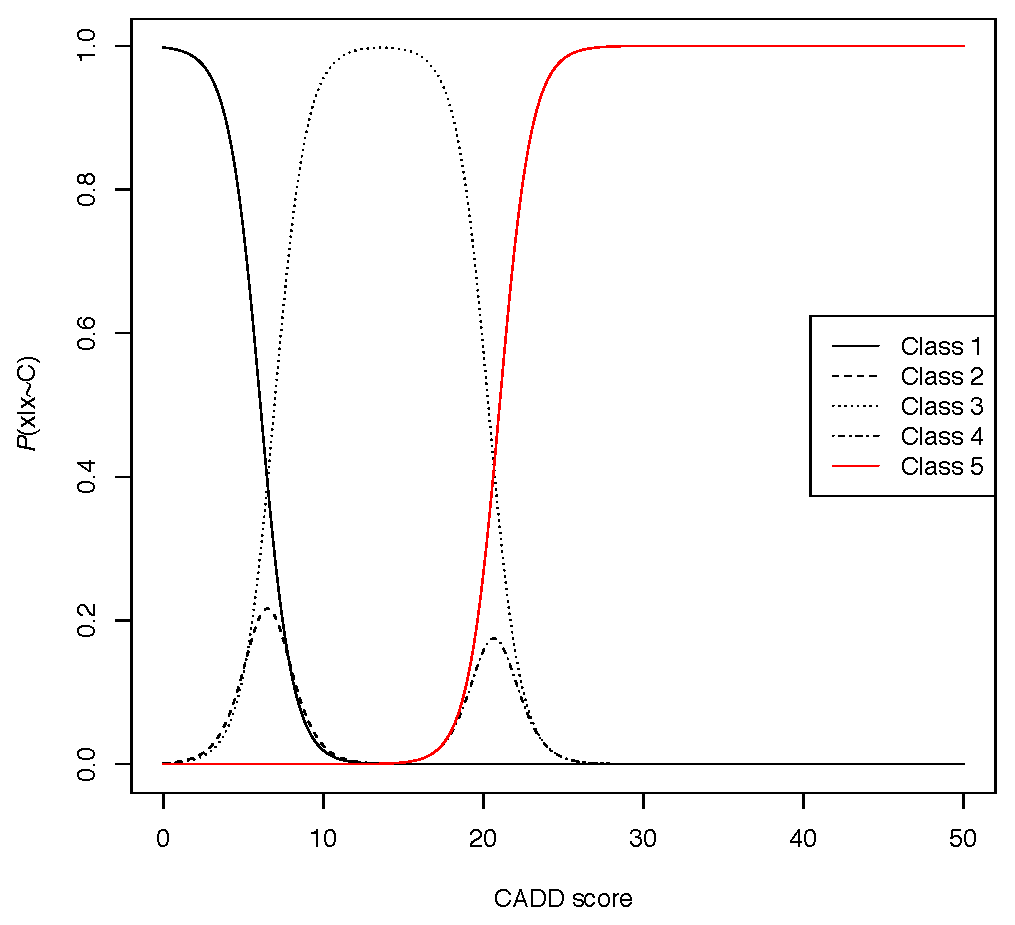
\includegraphics[width=1.00\linewidth]{img/caddmmr_regression}
  \caption[Probability that a CADD score belongs to a class]{
      \label{fig:caddmmr_regression} Probability that a CADD score will belong to a certain InSiGHT class.
      The inverse logit ($\text{logit}^{-1}$) was applied to each of the response variables.
      Classes 2 and 4 are dominated by class 3 under this model.
  }
\end{figure}

\subsection{Data availability}
The data and scripts used in this paper can be downloaded from: \url{http://molgenis.org/downloads/vdVelde_Kuiper_etal_2015/}

\section{Results}

\subsection{Exploratory data analysis}
We calculated the CADD scores for 2,744 MMR gene variants that were downloaded from the InSiGHT group LOVD (available at \url{http://chromium.liacs.nl/LOVD2/colon_cancer/}).
A total of 534 variants had to be omitted, either because converting the complementary DNA HGVS nomenclature\cite{den_Dunnen_2003} based notation to genomic DNA VCF (Variant Call Format version 4.0 \cite{Danecek_2011}) based notation failed (162 variants), or the CADD scores could not be unambiguously assigned (2 variants with \textsl{T$>$R} and \textsl{A$>$Y} substitutions), or because they had not yet been classified by the InSiGHT VIC (i.e., they were recent submissions, or not reported as germline variants [370 variants]).
See Figure~\ref{fig:flowchart} and \textsl{\nameref{methods}} for details.
The 2,210 remaining variants fell within one of the five classes: class 1 ($n$ = 151), class 2 ($n$ = 84), class 3 ($n$ = 751), class 4 ($n$ = 181), or class 5 ($n$ = 1,043).

\begin{figure*}[htb]
  \begin{center}
    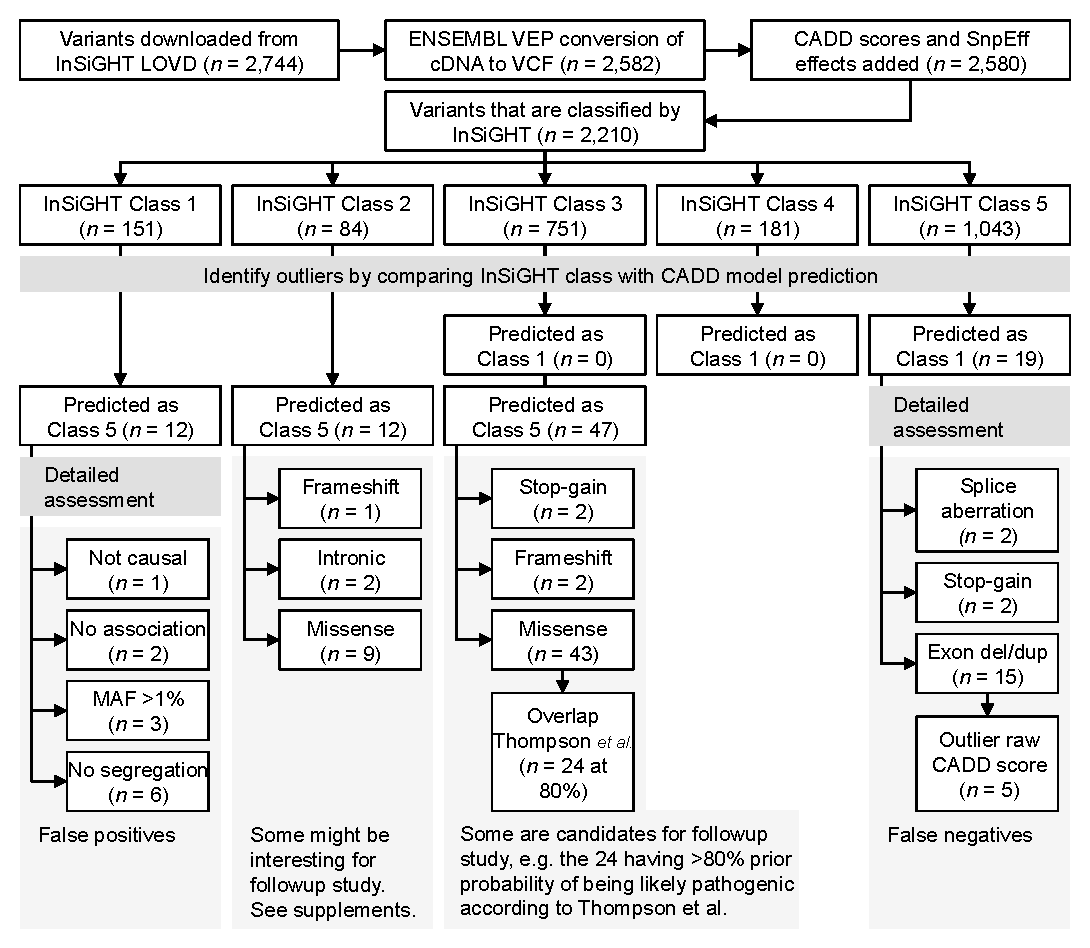
\includegraphics[width=1.00\linewidth]{img/caddmmr_flowchart}
  \end{center}
    \caption[Flowchart describing the analysis]{\label{fig:flowchart} Flowchart describing the steps and results of the analysis. \textsl{[Note: the original figure mentions 2,274 downloaded variants, this was corrected to 2,744 here.]}}
\end{figure*}

Overall, the CADD scaled C-score distributions for each class correlate with the InSiGHT classification (Spearman’s $\rho$ = 0.595, p $<$ 0.001).
In Figure~\ref{fig:beanplot}, the distribution of the scores per class is represented in a beanplot\cite{Kampstra_2008}.
See also Figures \ref{fig:caddmmr_mlh1}, \ref{fig:caddmmr_msh2}, \ref{fig:caddmmr_msh6} and \ref{fig:caddmmr_pms2} for CADD scores of the InSiGHT variants for each gene, using known variants identified in the Genome of the Netherlands\cite{Boomsma_2014,Francioli_2014} and 1000 Genomes\cite{McVean_2012} projects as population background reference.

\begin{figure}[htb]
\centering
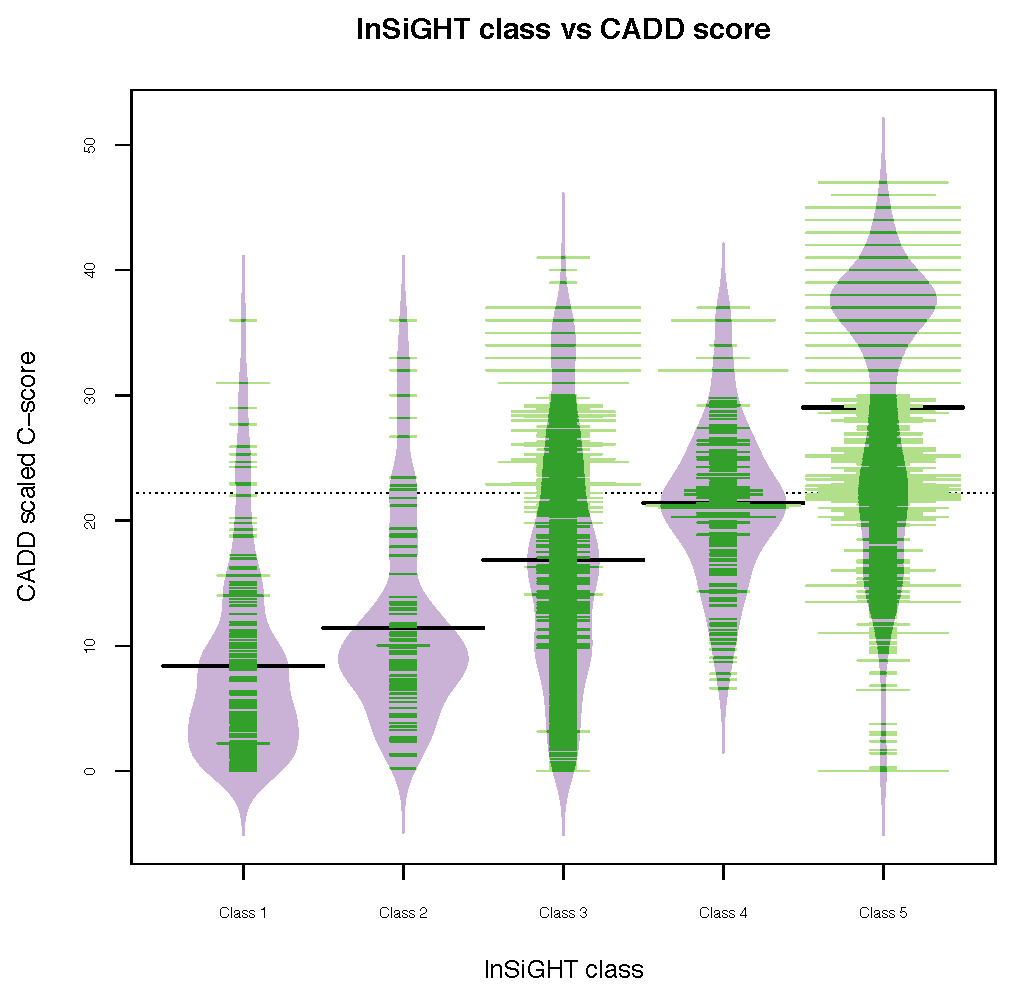
\includegraphics[width=1.0\linewidth]{img/caddmmr_beanplot}
\caption[Beanplot showing CADD score data and density]{
    \label{fig:beanplot}
    Beanplot\cite{Kampstra_2008} showing the data points (green) and density estimation (purple) of the scaled CADD C-score per InSiGHT class.
    The width of the green lines is relative to the number of data points at that score.
    Black horizontal lines indicate the mean per InSiGHT class; the dotted line shows the overall mean.
    The mean scores of classes 1-5 show a respective stepwise increase of 8.41 ($\sigma$ = 7.46), 11.44 ($\sigma$ = 7.72), 16.87 ($\sigma$ = 9.40), 21.41 ($\sigma$ = 6.13), and 29.04 ($\sigma$ = 10.28).
    The unclassified group (class 3) shows a flatter distribution than the other classes.}
\end{figure}

\begin{sidewaysfigure}
\centering
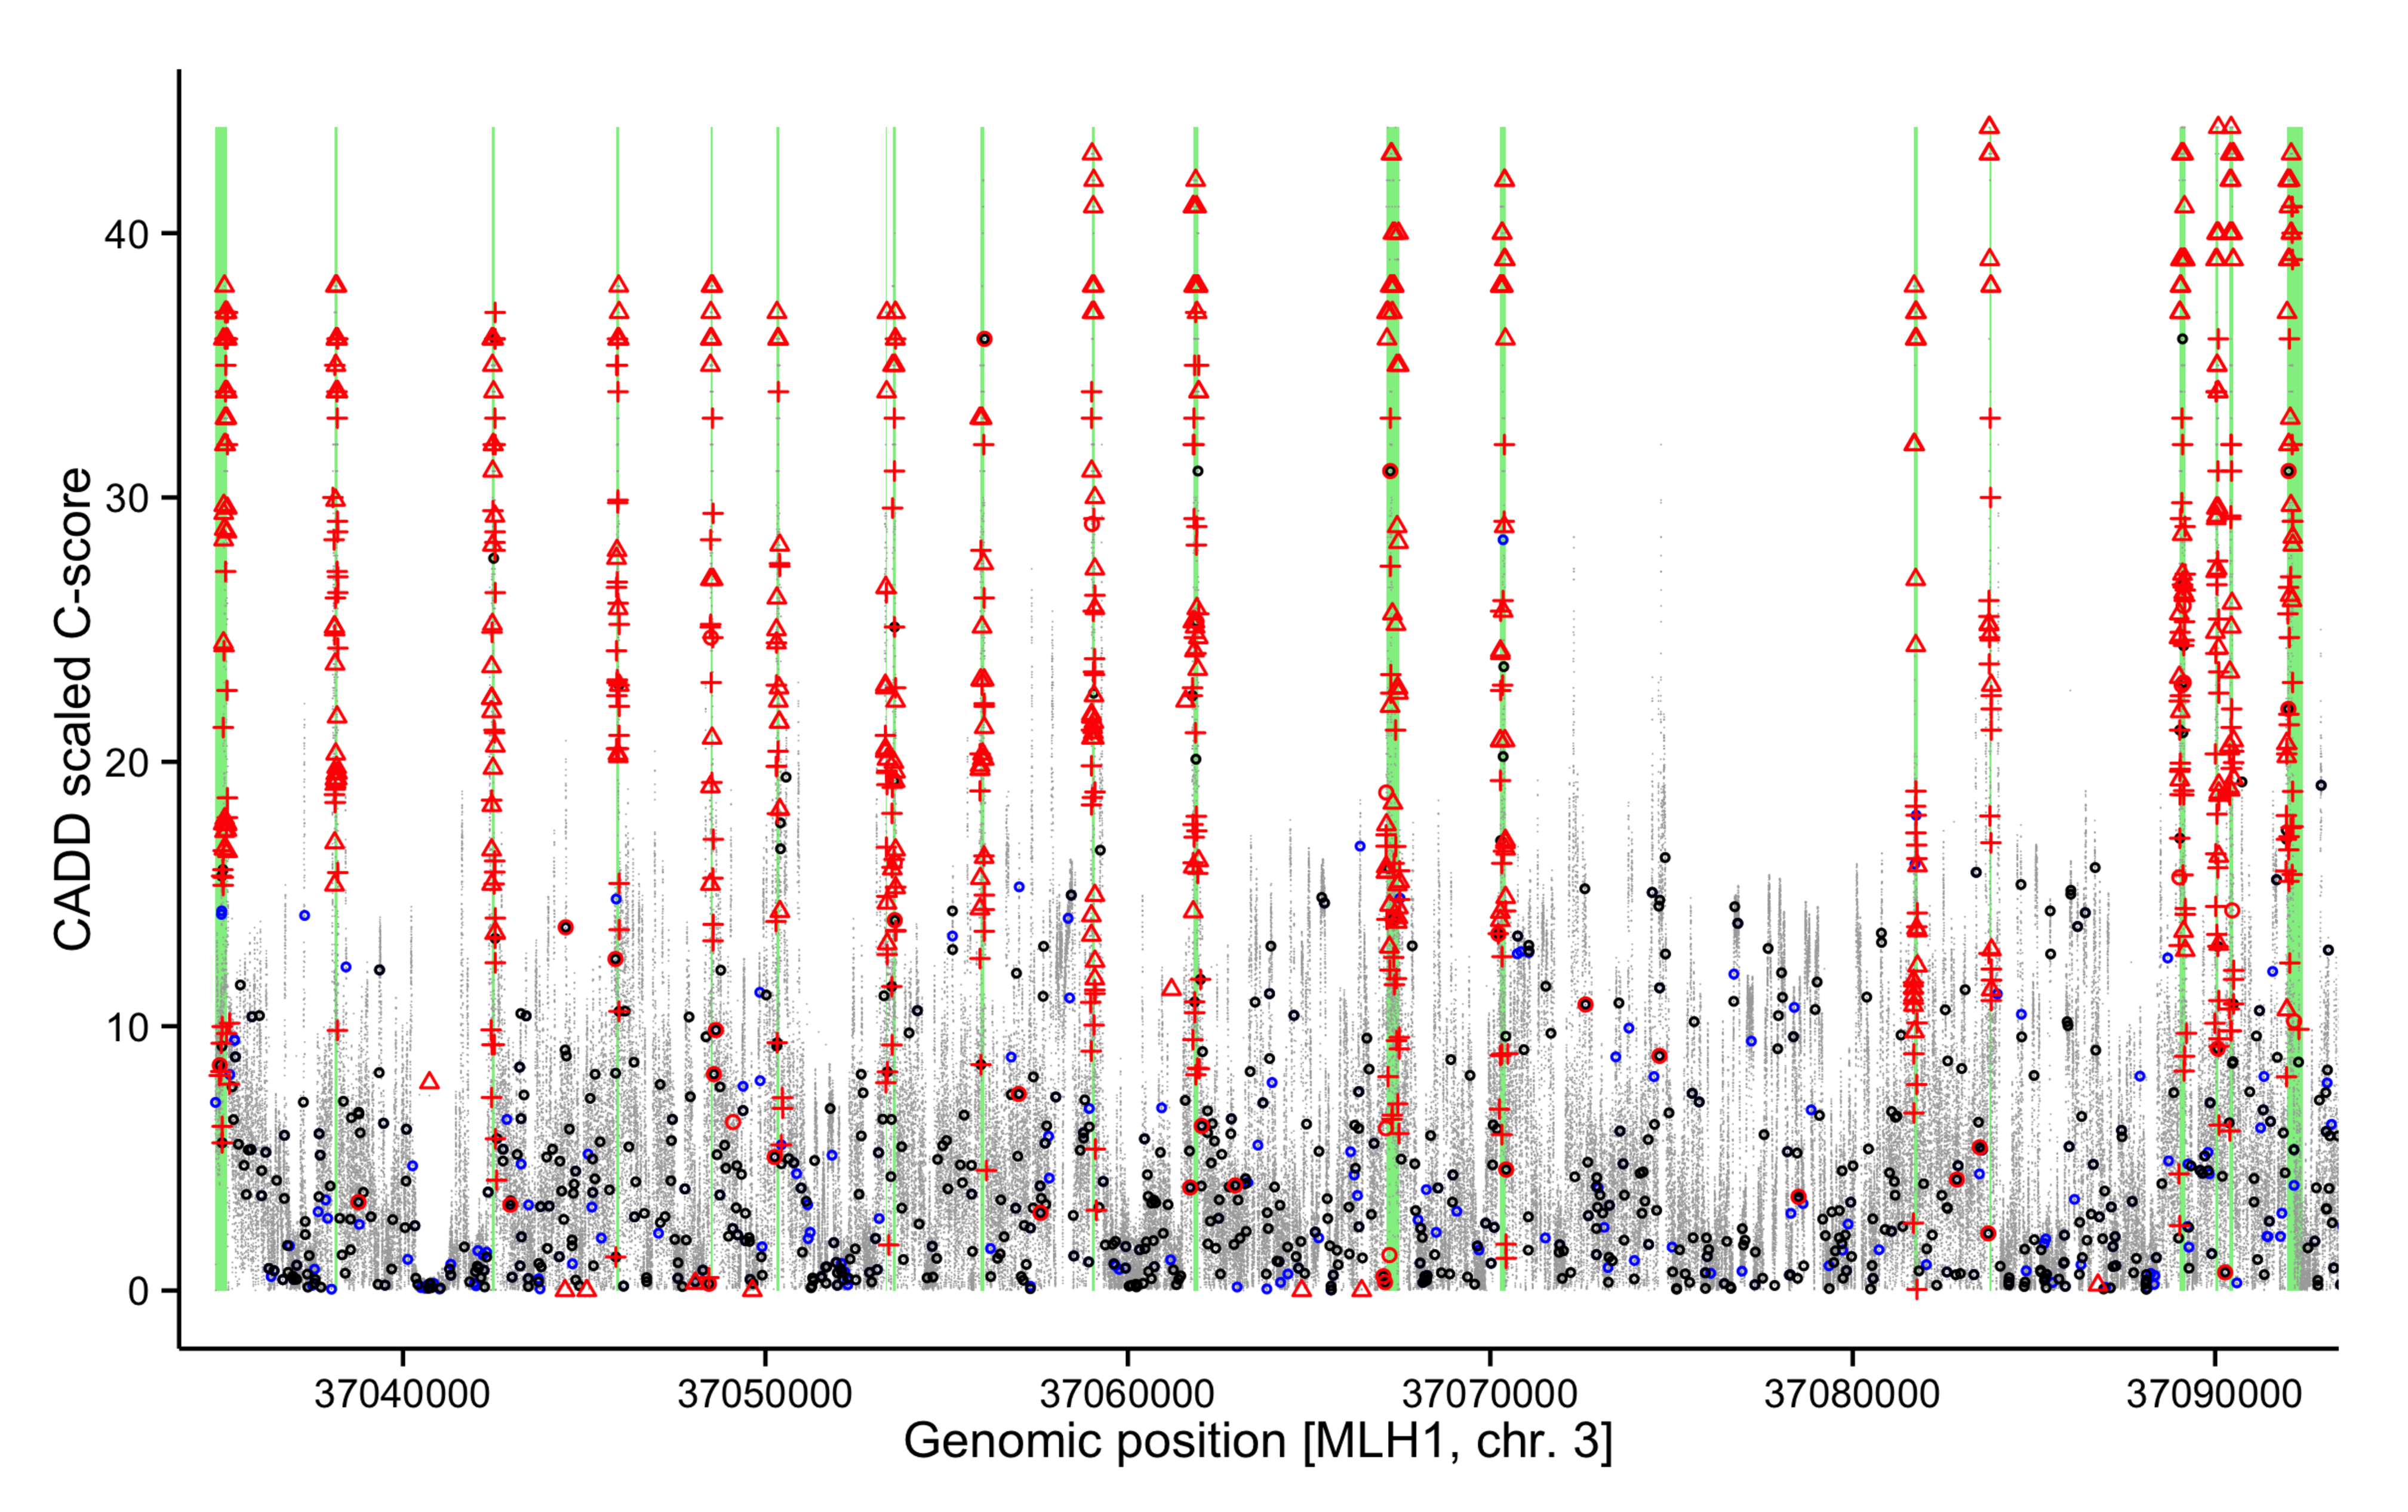
\includegraphics[width=1.0\linewidth]{img/caddmmr_mlh1}
\caption[CADD scaled C-scores for MLH1 gene]{CADD scaled C-scores vs. genomic coordinates for MLH1 gene variants. The green bands are the exons. Red are InSiGHT variants, where triangles represent class 5, circles class 1, and plusses class 2-4. The black circles are variants seen in 1000 Genomes\cite{McVean_2012}, blue circles are seen in the Genome of the Netherlands\cite{Boomsma_2014,Francioli_2014}. The gray dots represent all potential SNVs.}
\label{fig:caddmmr_mlh1}
\end{sidewaysfigure}

\begin{sidewaysfigure}
\centering
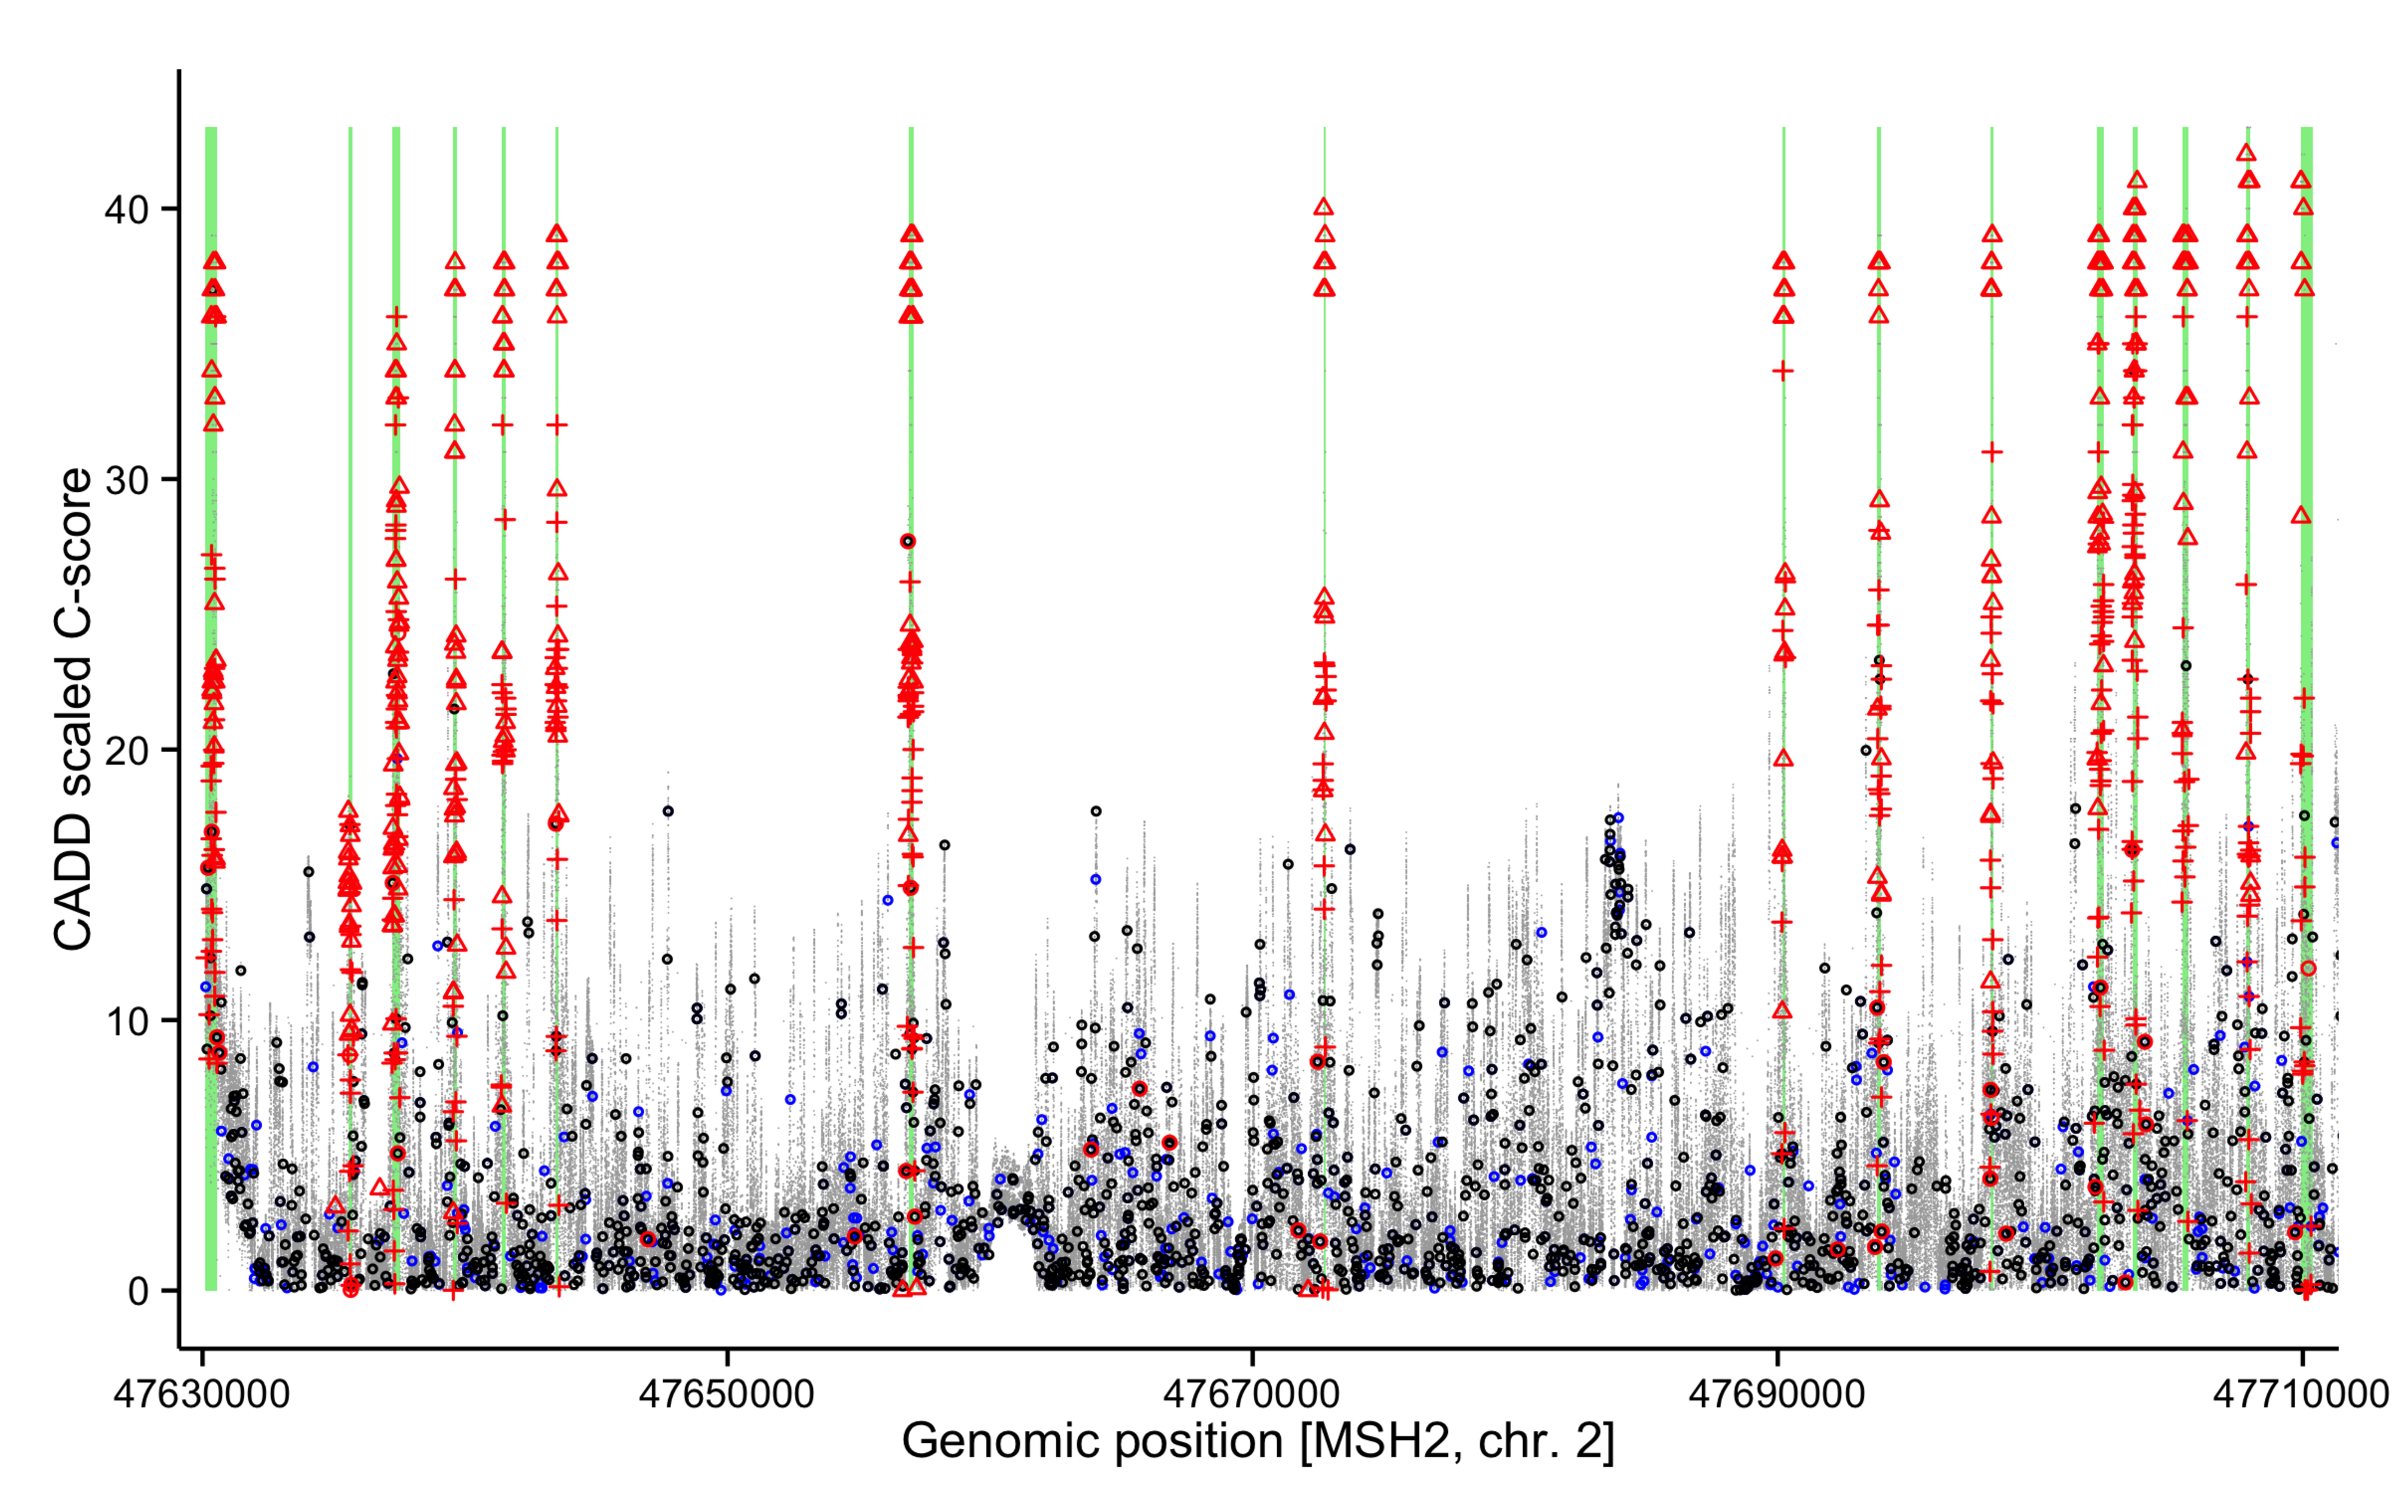
\includegraphics[width=1.0\linewidth]{img/caddmmr_msh2}
\caption[CADD scaled C-scores for MSH2 gene]{CADD scaled C-scores vs. genomic coordinates for MSH2 gene variants. The green bands are the exons. Red are InSiGHT variants, where triangles represent class 5, circles class 1, and plusses class 2-4. The black circles are variants seen in 1000 Genomes\cite{McVean_2012}, blue circles are seen in the Genome of the Netherlands\cite{Boomsma_2014,Francioli_2014}. The gray dots represent all potential SNVs.}
\label{fig:caddmmr_msh2}
\end{sidewaysfigure}

\begin{sidewaysfigure}
\centering
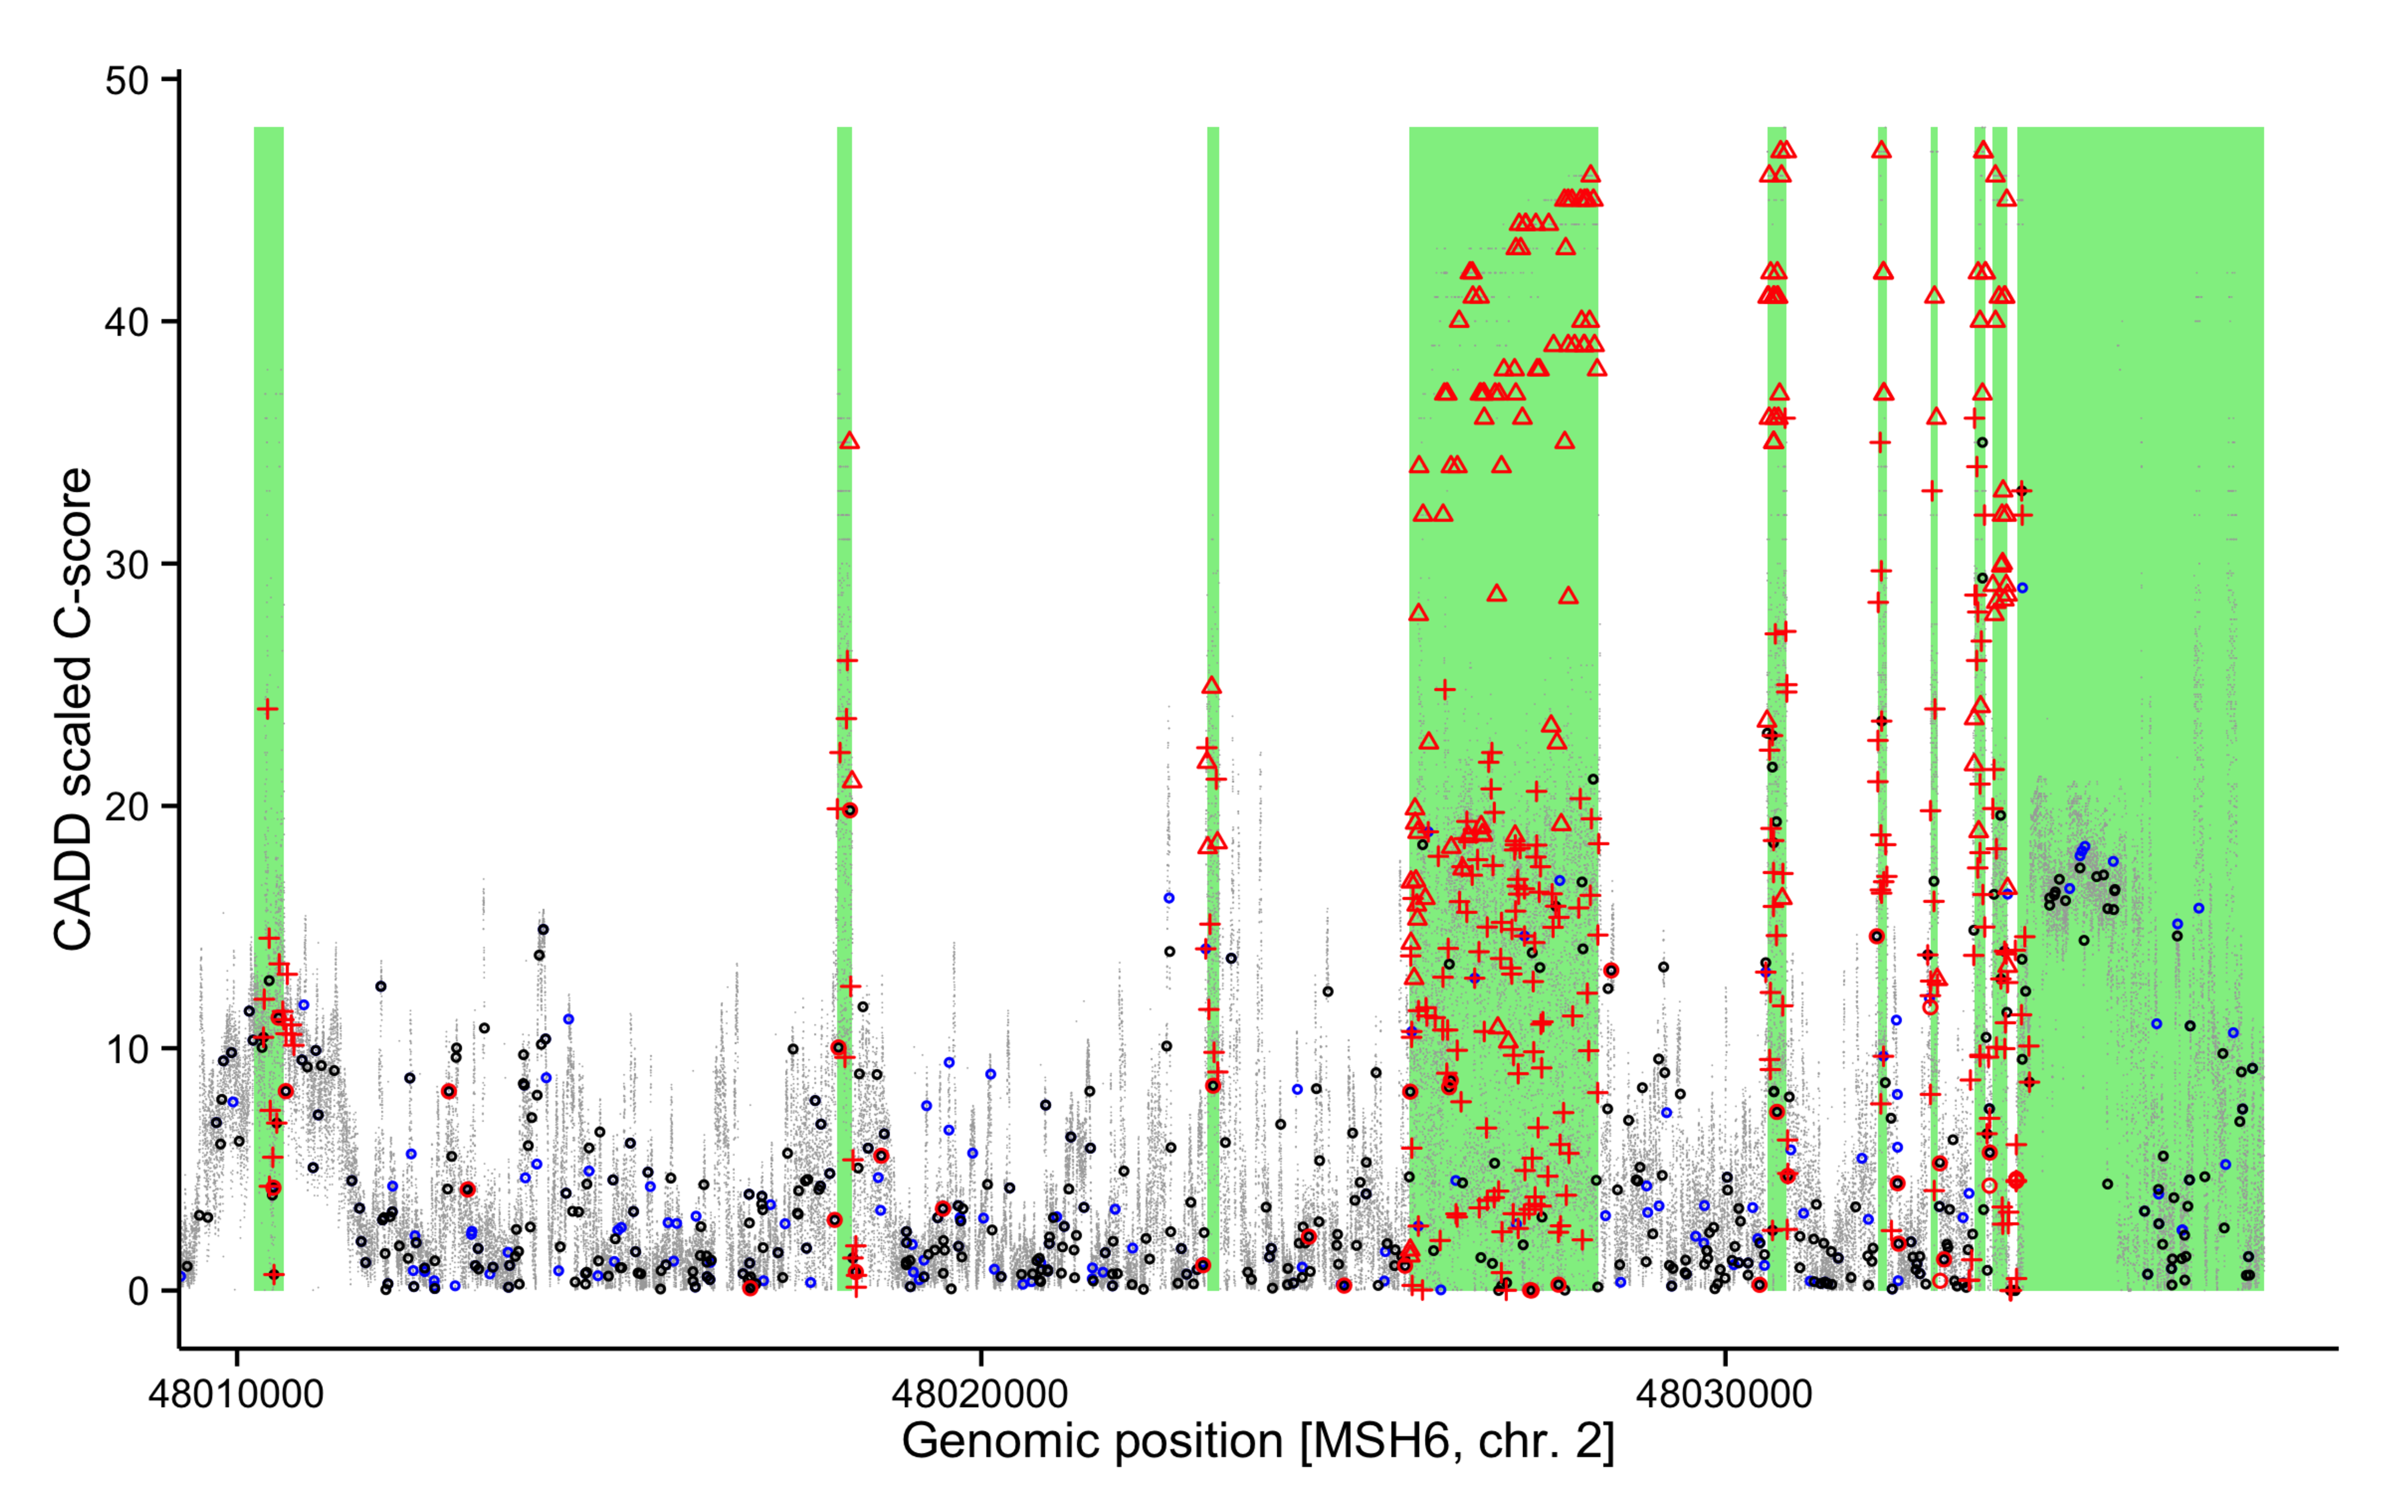
\includegraphics[width=1.0\linewidth]{img/caddmmr_msh6}
\caption[CADD scaled C-scores for MSH6 gene]{CADD scaled C-scores vs. genomic coordinates for MSH6 gene variants. The green bands are the exons. Red are InSiGHT variants, where triangles represent class 5, circles class 1, and plusses class 2-4. The black circles are variants seen in 1000 Genomes\cite{McVean_2012}, blue circles are seen in the Genome of the Netherlands\cite{Boomsma_2014,Francioli_2014}. The gray dots represent all potential SNVs.}
\label{fig:caddmmr_msh6}
\end{sidewaysfigure}

\begin{sidewaysfigure}
\centering
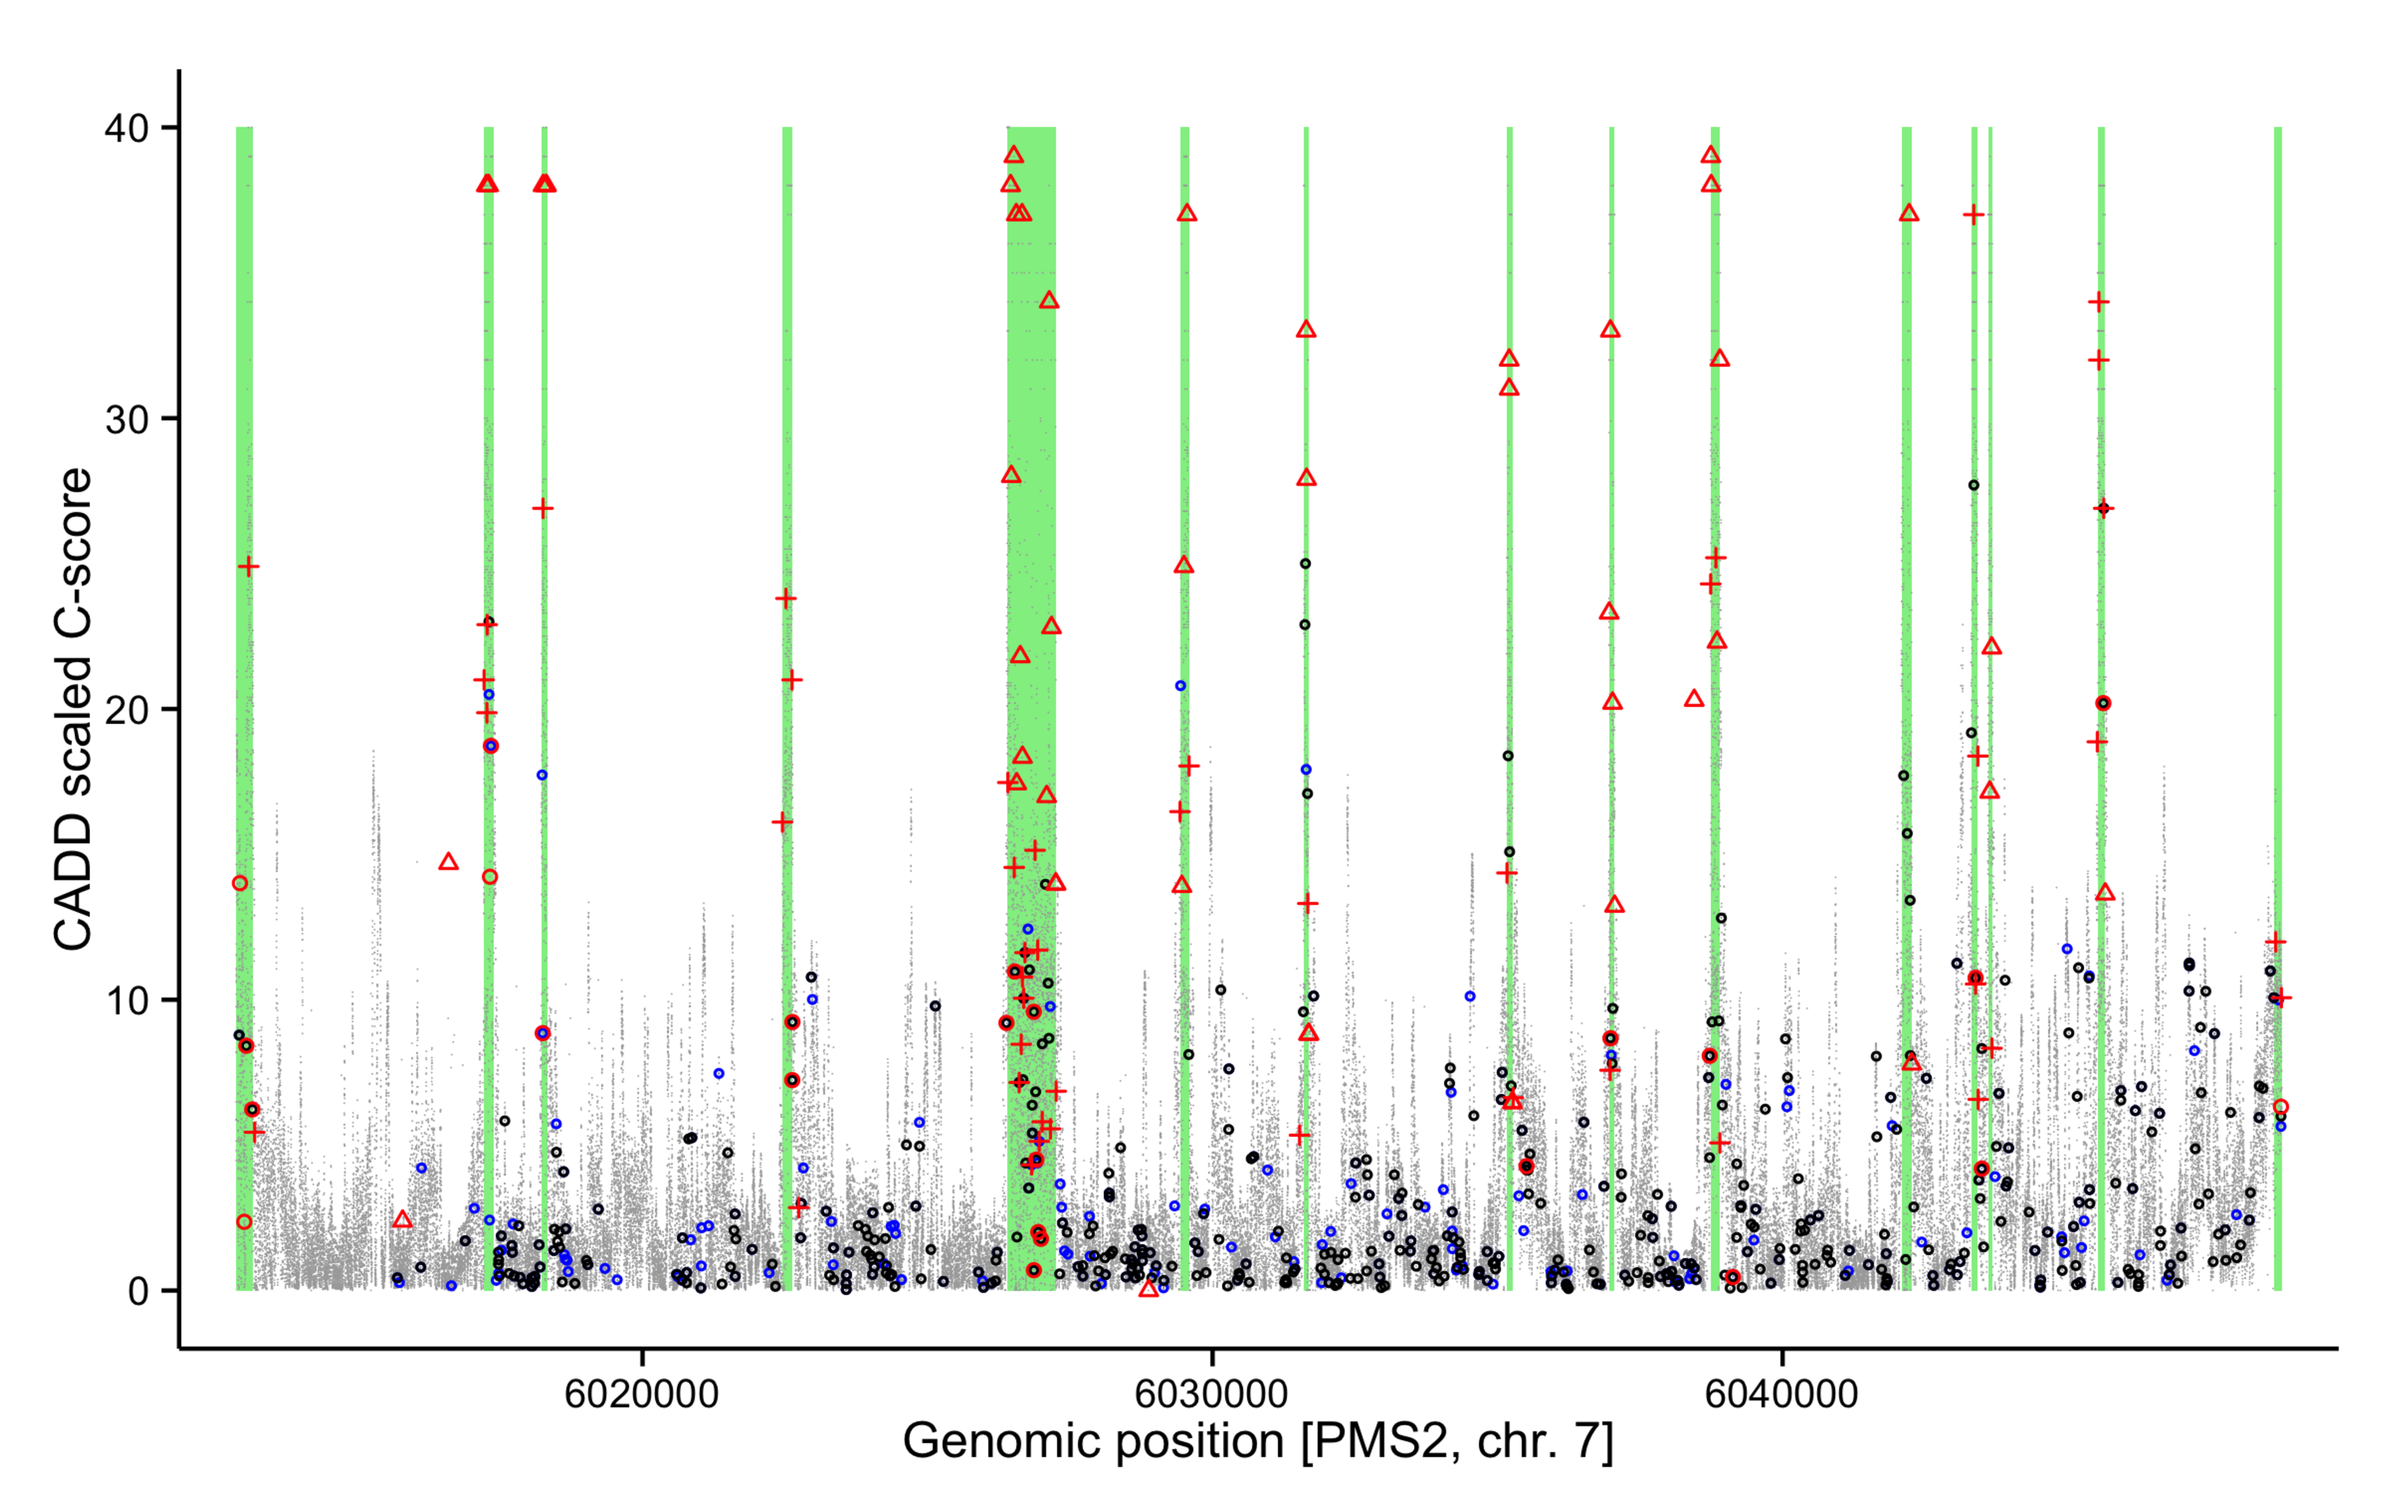
\includegraphics[width=1.0\linewidth]{img/caddmmr_pms2}
\caption[CADD scaled C-scores for PMS2 gene]{CADD scaled C-scores vs. genomic coordinates for PMS2 gene variants. The green bands are the exons. Red are InSiGHT variants, where triangles represent class 5, circles class 1, and plusses class 2-4. The black circles are variants seen in 1000 Genomes\cite{McVean_2012}, blue circles are seen in the Genome of the Netherlands\cite{Boomsma_2014,Francioli_2014}. The gray dots represent all potential SNVs.}
\label{fig:caddmmr_pms2}
\end{sidewaysfigure}


\subsection{Discrepancy assessment}
Using a Bayesian cumulative link model, we identified 108 (4.89\% of 2,210) cases for which a different class would be assigned (see \textsl{\nameref{methods}}).
Further analysis focused on the cases for which the nonpathogenic (class 1) and pathogenic (class 5) classifications were reversed, as these suggested major disagreements between CADD and the InSiGHT VIC verdict (see Table~\ref{table:caddmmr_reassigned}).
The explanations per variant for this analysis can be found in Table~\ref{table:caddmmr_explanations1} and Table~\ref{table:caddmmr_explanations2}.

\begin{table}[htb]
\begin{tabular}{ l r r r r r }
  ~ & \multicolumn{5}{c}{InSiGHT classification} \\\cline{2-6}
  CADD model & Class 1 & Class 2 & Class 3 & Class 4 & Class 5 \\
  \hline
  Class 1 & 135 & & & & 19 \\
  Class 2 & & 71 & & & \\
  Class 3 & 4 & 1 & 704 & 3 & 3 \\
  Class 4 & & & & 171 & \\
  Class 5 & 12 & 12 & 47 & 7 & 1021 \\
  \hline
\end{tabular}
\caption[Number of InSiGHT variants reassigned]{\label{table:caddmmr_reassigned} Number of InSiGHT variants reassigned to alternative classes according to the cumulative link model fitted on CADD scores.}
\end{table}

\linespread{1.00} % need to squeeze a bit to fit these tables nicely

\begin{table}
\footnotesize
\begin{tabulary}{\linewidth}{LLRRL}
  \mbox{Gene~~~~~~~~~~~} & \mbox{Variant~~~~~~~~~~~~~~~~~~~~~~~~~~~~~} & InSiGHT class & CADD-based class & Explanation \\
  \hline
  \rule{0pt}{1.5ex}MLH1 & c.394G$>$C & 1 & 5 & Attenuated protein function, but does not cause Lynch syndrome. Multifactorial likelihood analysis posterior probability $<$0.001 \\
  \rule{0pt}{1.5ex}MLH1 & c.1852\_ 1853delinsGC & 1 & 5 & Low risk, not associated with Lynch. Multifactorial likelihood analysis posterior probability $<$0.001 \\
  \rule{0pt}{1.5ex}MLH1 & c.803A$>$G & 1 & 5 & Multiple microsatellite stable tumours and does not segregate with disease. Multifactorial likelihood analysis posterior probability $<$0.001 \\
  \rule{0pt}{1.5ex}MLH1 & c.977T$>$C & 1 & 5 & Multiple microsatellite stable tumours and does not segregate with disease. Multifactorial likelihood analysis posterior probability $<$0.001 \\
  \rule{0pt}{1.5ex}MLH1 & c.1853A$>$C & 1 & 5 & Multiple microsatellite stable tumours and does not segregate with disease. Multifactorial likelihood analysis posterior probability $<$0.001 \\
  \rule{0pt}{1.5ex}MLH1 & c.2146G$>$A & 1 & 5 & Multiple microsatellite stable tumours and does not segregate with disease. Multifactorial likelihood analysis posterior probability $<$0.001 \\
  \rule{0pt}{1.5ex}MLH1 & c.1151T$>$A & 1 & 5 & Population minor allele frequency $>$1\% \\
  \rule{0pt}{1.5ex}MLH1 & c.2152C$>$T & 1 & 5 & Population minor allele frequency $>$1\% \\
  \rule{0pt}{1.5ex}MSH2 & c.1077-10T$>$C & 1 & 5 & Population minor allele frequency $>$1\% \\
  \rule{0pt}{1.5ex}MLH1 & c.1799A$>$G & 1 & 5 & Does not segregate with disease. Multifactorial likelihood analysis posterior probability $<$0.001 \\
  \rule{0pt}{1.5ex}MLH1 & c.790+10A$>$G & 1 & 5 & Does not cause splicing aberration and does not segregate with disease. Multifactorial likelihood analysis posterior probability $<$0.001 \\
  \rule{0pt}{1.5ex}MSH2 & c.593A$>$G & 1 & 5 & May be low-moderate risk, but certainly not high-risk associated with Lynch \\
  \rule{0pt}{1.5ex}MSH6 & c.642C$>$A & 5 & 1 & Stop-gain variant causing protein truncation \\
  \hline
\end{tabulary}
\caption[Explanations according to InSiGHT, pt. 1/2]{\label{table:caddmmr_explanations1} Overview of explanations according to InSiGHT why the cumulative link model based on CADD scores encountered certain false positives and false negatives, pt. 1/2.}
\end{table}

\begin{table}
\footnotesize
\begin{tabulary}{\linewidth}{LLRRL}
  \mbox{Gene~~~~~~~~~~~} & \mbox{Variant~~~~~~~~~~~~~~~~~~~~~~~~~~~~~~~~~~~~~~} & InSiGHT class & CADD-based class & Explanation \\
  \hline
  \rule{0pt}{1.5ex}MSH6 & c.642C$>$G & 5 & 1 & Stop-gain variant causing protein truncation \\
  \rule{0pt}{1.5ex}MSH2 & c.212-478T$>$G & 5 & 1 & Splicing aberration introduces premature termination codon (also missed by SnpEff) \\
  \rule{0pt}{1.5ex}MSH2 & c.646-3T$>$G & 5 & 1 & Splicing aberration introduces premature termination codon \\
  \rule{0pt}{1.5ex}MSH2 & c.367-480\_ 645+644del & 5 & 1 & Deletion of Exon 3 \\
  \rule{0pt}{1.5ex}MLH1 & c.307-1420\_ 380+624del & 5 & 1 & Deletion of Exon 4 \\
  \rule{0pt}{1.5ex}MLH1 & c.307-820\_ 380+896del & 5 & 1 & Deletion of Exon 4 \\
  \rule{0pt}{1.5ex}MLH1 & c.381-415\_ 453+733del & 5 & 1 & Deletion of Exon 5 \\
  \rule{0pt}{1.5ex}MLH1 & c.454-665\_ 545+49del & 5 & 1 & Deletion of Exon 6 (raw score of 527) \\
  \rule{0pt}{1.5ex}MLH1 & c.1039-675\_ 1409+26del & 5 & 1 & Deletion of Exon 12 (raw score of 361) \\
  \rule{0pt}{1.5ex}MLH1 & c.1039-2329\_ 1409+827del & 5 & 1 & Deletion of Exon 12 (raw score of 353) \\
  \rule{0pt}{1.5ex}MLH1 & c.1732-2243\_ 1896+404del & 5 & 1 & Deletion of Exon 16 \\
  \rule{0pt}{1.5ex}MSH2 & c.1077-135\_ 1276+119dup & 5 & 1 & Duplication of Exon 7 (also missed by SnpEff) \\
  \rule{0pt}{1.5ex}MSH2 & c.1077-220\_ 1276+6245del & 5 & 1 & Deletion of Exon 7 \\
  \rule{0pt}{1.5ex}MSH2 & c.1277-572\_ 1386+2326del & 5 & 1 & Deletion of Exon 8 (raw score of 464) \\
  \rule{0pt}{1.5ex}PMS2 & c.804-?\_ 903+?del & 5 & 1 & Deletion of Exon 8 \\
  \rule{0pt}{1.5ex}PMS2 & c.804-?\_ 2006+?del & 5 & 1 & Deletion of Exons 8-11 \\
  \rule{0pt}{1.5ex}PMS2 & c.989-296\_ 1144+706del & 5 & 1 & Deletion of Exon 10 (raw score of 527) \\
  \rule{0pt}{1.5ex}PMS2 & c.2276-113\_ 2445+1596del & 5 & 1 & Deletion of Exon 14 \\
  \hline
\end{tabulary}
\caption[Explanations according to InSiGHT, pt. 2/2]{\label{table:caddmmr_explanations2} Overview of explanations according to InSiGHT why the cumulative link model based on CADD scores encountered certain false positives and false negatives, pt. 2/2.}
\end{table}

\linespread{1.05} % and back to normal

\subsection{False positives}
We identified 12 variants (0.54\% of 2,210) that were classified as nonpathogenic (class 1) by the InSiGHT VIC, but they were predicted to be pathogenic (class 5) according to the CADD-based cumulative link model (see \textsl{\nameref{methods}}).
Re-examination of the available data for these variants strongly supports the original InSiGHT classification based on the following evidence:
\begin{itemize}
  \item Segregation data is inconsistent with the variant being a dominant, high-risk, pathogenic sequence variant in pedigrees (likelihood ratio $\leq$0.01).
  \item Variant with reported frequency $\geq$1\% in the general population (1000 Genomes Project), and no evidence that variant is a founder mutation.
  \item These are not high-risk variants that are uniquely associated with Lynch syndrome (they have also been seen in individuals who do not meet the international criteria for Lynch syndrome).
  \item Variant leads to a known attenuated protein function, but this does not cause Lynch syndrome (it has also been seen in healthy individuals and there is a lack of evidence for MMR deficiency as shown by MSI and immunohistochemical testing).
\end{itemize}
Although these explanations are specific to Lynch syndrome-related variants, they indicate that CADD might overestimate the general pathogenicity of some variants.
Most overestimations could be easily resolved in a clinical Standard Operating Procedure (SOP) by using population allele frequency as a filter or incorporating the use of patient pedigree analysis data; these are already common practices in many clinical laboratories.
The remainder could be resolved by incorporating more in-depth findings from validated protein functional assays or from risk estimates based on large, well-designed, case-control studies that consider cohort size, geography/ethnicity, and quality control measures\cite{Thompson_2013a}.
An evaluation of likely not pathogenic (class 2) variants predicted to be pathogenic (class 5) can be found in Table \ref{table:caddmmr_vic2to5}.

\begin{sidewaystable}
\small
\begin{tabulary}{\linewidth}{LLLLL}
  Gene & Variant & AA change & Probability & VIC justification \\
  \hline
  \rule{0pt}{2.5ex}MLH1 & c.117-43\_ 117-39del & intronic & 0.99 & Intronic substitution with no associated splicing aberration, tested with NMD inhibitors \\
  \rule{0pt}{2.5ex}MLH1 & c.845C$>$G & A282G & 0.92 &  Posterior probability 0.001-0.049 \\
  \rule{0pt}{2.5ex}MLH1 & c.885-24T$>$A & intronic & 0.81 & Intronic substitution with no effect on splicing and MAF 0.01-1\% \\
  \rule{0pt}{2.5ex}MLH1 & c.974G$>$A & R325Q & 0.99 &  Posterior probability 0.001-0.049 \\
  \rule{0pt}{2.5ex}MLH1 & c.1742C$>$T & P581L & 0.55 & Posterior probability 0.001-0.049. No CMMRD phenotype with co-occurrence and MAF 0.01-1\% \\
  \rule{0pt}{2.5ex}MLH1 & c.1808C$>$G & P603R & 0.99 & Posterior probability 0.001-0.049 \\
  \rule{0pt}{2.5ex}MLH1 & c.1820T$>$A & L607H & 0.99 &  Posterior probability 0.001-0.049 \\
  \rule{0pt}{2.5ex}MSH2 & c.991A$>$G & N331D & 0.69 & Posterior probability 0.001-0.049 \\
  \rule{0pt}{2.5ex}MSH2 & c.1730T$>$C & I577T & 0.86 & Posterior probability 0.001-0.049 \\
  \rule{0pt}{2.5ex}MSH2 & c.2500G$>$A & A834T & 0.99 &  Posterior probability 0.001-0.049 \\
  \rule{0pt}{2.5ex}MSH6 & c.3488A$>$T & E1163V & 0.92 & MAF $>$1\% in specific population \\
  \rule{0pt}{2.5ex}MSH6 & c.4068\_ 4071dup & Lys1358 Aspfs*2 & 0.99 & MAF $>$1\% in specific ethnic group \\
  \hline
\end{tabulary}
\caption[Variants of class 2 for which class 5 is the predicted]{\label{table:caddmmr_vic2to5} Variants of class 2 (likely benign) for which class 5 (pathogenic) is the predicted class according to the CADD-based model. Posterior probabilities are derived from a multifactorial likelihood analysis.}
\end{sidewaystable}

\subsection{False negatives}
We identified 19 cases (0.86\% of 2,210) for which the cumulative link model predicted the respective variants to be class 1, whereas InSiGHT scored them as class 5.
This indicates that the model might also underestimate effects.
Similar to the approach to the false-positives, outlined above, our re-examination of these variants supported the original InSiGHT classification.

CADD scores are developed for scoring any possible human SNVs or small indels\cite{Kircher_2014}.
It was therefore expected that large structural variants would be missed or inaccurately scored (for 5/15 structural variants) by CADD.
To simplify the interpretation, the scaled C-scores are based on the rank of the C-score relative to all the C-scores for 8.6 billion possible SNVs.
Typical variant C-scores in this study ranged from -4 to 14, while the five structural variants in question scored very highly (between 350 and 550), whereas was expected considering the likely pathogenicity of exon deletions relative to missense variants or codon deletions, for example.
However, the scaling algorithm seems to fail for such extreme C-scores, and this results in reverting the score for the respective variant into a very low scaled C-score instead.
We applied SnpEff\cite{Cingolani_2012} as a second-tier test.
This tool has been developed to annotate and predict the effects of variants in genes in a robust and qualitative way, thereby complementing the quantitative nature of CADD scores.
Using SnpEff, we were able to correct 17 of the 19 false-negative cases.
SnpEff recognized 14 of the 15 structural variants, most as "EXON\_DELETED", one of two splice aberrations as "FRAME\_SHIFT", and two of two truncating mutations as "STOP\_GAINED".
These effect types are annotated as HIGH impact in SnpEff, in contrast to MODIFIER, LOW or MODERATE effect types.
By using SnpEff information, we have shown that CADD results should be complemented by this tool, or a comparable tool, to compensate for sporadic underestimations.
See Figure~\ref{fig:caddmmr_snpeffvscadd} for an overview of SnpEff variant effect predictions in relation to CADD scores and InSiGHT classifications.

\begin{sidewaysfigure}
\centering
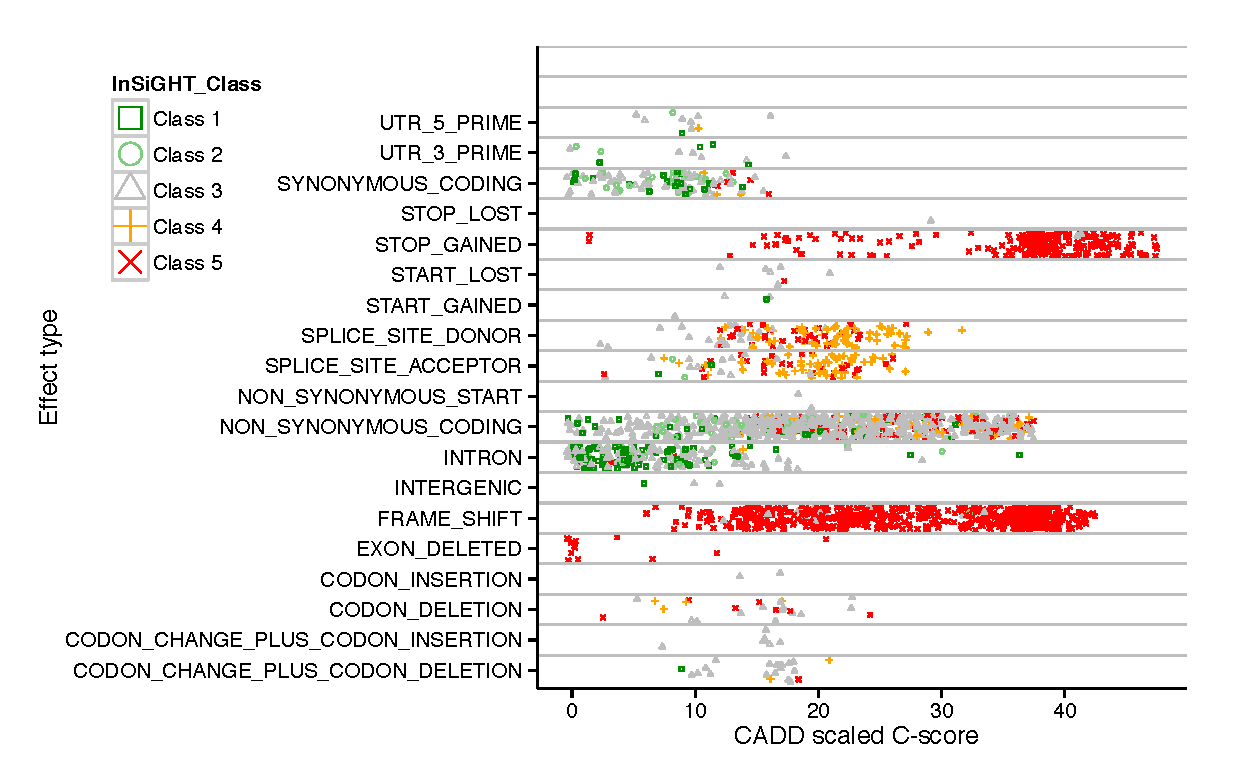
\includegraphics[width=1.0\linewidth]{img/caddmmr_snpeffvscadd}
\caption[SnpEff effect vs. CADD score]{Primary SnpEff effect prediction vs. CADD scaled C-score, with InSiGHT classifications colored.}
\label{fig:caddmmr_snpeffvscadd}
\end{sidewaysfigure}

\subsection{Variants of unknown significance}
Class 3 mainly contains variants for which insufficient clinical or molecular data are available, but also a limited number of variants that have discordant findings (i.e., are resistant to classification).
Most of these variants can easily be assigned to another class as soon as more data become available.
As expected, the distribution of the CADD scores for class 3 variants, as visualized in Figure~\ref{fig:beanplot}, is much flatter than the distributions for the other classes.
Matching the CADD score of each class 3 variant to the distributions of the other classes (and thus, the likelihood of belonging to one of them) allows us to propose an endpoint classification that is, according to the model, more likely than belonging to class 3 for these variants.
In other words, we can suggest prioritization of a variant for reclassification (using additionally obtained clinical and molecular evidence) when its CADD score deviates far enough from this mean, reaching a score that falls into the distributions of known nonpathogenic or pathogenic variant classes (see \textsl{\nameref{methods}}).

We performed this analysis and 47 variants (2.13\% of 2,210) that the InSiGHT VIC classified as class 3 (uncertain significance) had CADD scores $\geq$34, which fell in the $>$99\% probability range for known class 5 (pathogenic) variants (see Figure~\ref{fig:caddmmr_regression}).
Of these 47 variants, 43 were missense with a mean CADD score of 35.33 ($\sigma$ = 1.04, 27 in \textit{MLH1}, 10 in \textit{MSH2}, four in \textit{MSH6} and two in \textit{PMS2}).
The remaining four were truncating mutations: two stop-gain variants (c.2250C$>$A and c.2250C$>$G, both with a CADD score of 41), and two frameshift variants (c.2252\_2253del and c.2262del) with CADD scores of 39 and 40.
These four variants are all located in the \textit{MLH1} gene; they were classified as class 3 by the InSiGHT VIC due to insufficient evidence, because the stop codons are introduced in the last exon (19) and are located outside any known functional domains.

We compared these findings with the previous use of a prediction model\cite{Thompson_2013b} on 481 substitutions\cite{Thompson_2013a} of uncertain effect.
In this analysis, 173 InSiGHT missense variants of uncertain significance (class 3) with a $>$80\% probability in favor of pathogenicity, were prioritized for further investigation using multifactorial likelihood analysis.
The model calibrated a combination of in silico tools to predict probabilities of pathogenicity, which is conceptually somewhat similar to the way CADD scores are constructed, except here the model was specifically for MMR gene variants associated with Lynch syndrome.

By comparing the two sets of results, that is, the 173 previously identified variants with our 43 prioritized variants, we found an overlap of 24 variants(see Table~\ref{table:caddmmr_overlap}).
Since they were called by both models, we consider these 24 missense variants to be the most urgent candidates for further research to determine their pathogenicity.
Of the remaining 19 variants prioritized uniquely by CADD, 17 had been evaluated before with prior probabilities of pathogenicity ranging from 7\% (MSH2:c.1418C$>$T) to 74-76\% (MLH1: c.85G$>$T, c.187G$>$A, c.299G$>$A, c.794G$>$A, c.955G$>$A, c.1976G$>$A, PMS2: 137G$>$A).

\begin{table}[h]
\begin{tabular}{ l l l r l }
  Gene & Variant & AA ch. & Previous\cite{Thompson_2013b} & Here\\
  \hline
  \rule{0pt}{2.5ex}MLH1 & c.1037A$>$G & Q346R & 0.95 & 0.99 \\
  \rule{0pt}{2.5ex}MLH1 & c.109G$>$A & E37K & 0.87 & 0.99 \\
  \rule{0pt}{2.5ex}MLH1 & c.112A$>$G & N38D & 0.94 & 0.99 \\
  \rule{0pt}{2.5ex}MLH1 & c.125C$>$T & A42V & 0.96 & 0.99 \\
  \rule{0pt}{2.5ex}MLH1 & c.184C$>$A & Q62K & 0.88 & 0.99 \\
  \rule{0pt}{2.5ex}MLH1 & c.1918C$>$T & P640S & 0.82 & 0.99 \\
  \rule{0pt}{2.5ex}MLH1 & c.1919C$>$T & P640L & 0.93 & 0.99 \\
  \rule{0pt}{2.5ex}MLH1 & c.304G$>$A & E102K & 0.87 & 0.99 \\
  \rule{0pt}{2.5ex}MLH1 & c.307G$>$C & A103P & 0.97 & 0.99 \\
  \rule{0pt}{2.5ex}MLH1 & c.331G$>$C & A111P & 0.97 & 0.99 \\
  \rule{0pt}{2.5ex}MLH1 & c.347C$>$A & T116K & 0.93 & 0.99 \\
  \rule{0pt}{2.5ex}MLH1 & c.65G$>$C & G22A & 0.89 & 0.99 \\
  \rule{0pt}{2.5ex}MLH1 & c.67G$>$A & E23K & 0.86 & 0.99 \\
  \rule{0pt}{2.5ex}MLH1 & c.74T$>$C & I25T & 0.86 & 0.99 \\
  \rule{0pt}{2.5ex}MLH1 & c.80G$>$C & R27P & 0.97 & 0.99 \\
  \rule{0pt}{2.5ex}MLH1 & c.925C$>$T & P309S & 0.83 & 0.99 \\
  \rule{0pt}{2.5ex}MSH2 & c.1799C$>$T & A600V & 0.96 & 0.99 \\
  \rule{0pt}{2.5ex}MSH2 & c.1826C$>$T & A609V & 0.96 & 0.99 \\
  \rule{0pt}{2.5ex}MSH2 & c.2064G$>$A & M688I & 0.89 & 0.99 \\
  \rule{0pt}{2.5ex}MSH2 & c.2141C$>$T & A714V & 0.87 & 0.99 \\
  \rule{0pt}{2.5ex}MSH2 & c.2168C$>$T & S723F & 0.88 & 0.99 \\
  \rule{0pt}{2.5ex}MSH2 & c.2187G$>$T & M729I & 0.88 & 0.99 \\
  \rule{0pt}{2.5ex}MSH2 & c.529G$>$A & E177K & 0.86 & 0.99 \\
  \rule{0pt}{2.5ex}MSH6 & c.3682G$>$C & A1228P & 0.97 & 0.99 \\
  \hline
\end{tabular}
\caption[The 24 variants predicted to be likely pathogenic]{\label{table:caddmmr_overlap} The 24 variants that are still uncertain and predicted by bioinformatic tools to be likely pathogenic, according to the probabilities of the MAPP + PolyPhen2 calibrated model\cite{Thompson_2013b} and the CADD model.}
\end{table}

We also compared a CADD-based binary classifier for missense variants with the multifactorial likelihood model\cite{Thompson_2013b}.
The multifactorial model's combination of customized MAPP + PolyPhen2 was found to perform best with an $R^2$ (the coefficient of determination) of 0.62 and an area under curve receiver operating characteristic (ROC-AUC) of 93\%, when distinguishing classes 1 + 2 collapsed as "likely not pathogenic" versus classes 4 + 5 collapsed as "likely pathogenic".
As a comparison, and not related to the cumulative link model, we performed a binary classification using CADD scores and obtained a ROC-AUC of 85\%, showing that while a CADD-based binary classifier for MMR gene missense variants performs reasonably well, it does not perform as well as a disease-specific model.

\section{Discussion}
We investigated the use of CADD scores for the prediction of clinical classifications by comparing them with a high quality clinical data set developed by the InSiGHT VIC, which is based on quantitative and qualitative interpretation of both clinical and molecular data.
Generally, the CADD model predictions fitted the InSiGHT classification.
Out of the 2,210 variants we tested and classified by InSiGHT, we identified 12 (0.54\%) nonpathogenic (class 1) variants that the CADD model predicted to be pathogenic (class 5), and 19 variants (0.86\%) of class 5 that CADD predicted to be class 1.
The difference could be explained by two considerations: the CADD model was not designed to classify large structural or splice-site variants (55\% of all the discordant cases, 89\% of the false-negatives), and the clinical observations, population allele frequencies, and experimental molecular data sometimes convincingly suggested an alternative interpretation (39\% of all discordant cases, 100\% of the false-positives).
CADD’s main underestimation of pathogenicity was due to its inability to accurately predict the effects of whole exon deletions or duplications.
In five such cases, the C-score was in fact extremely high, but this was not translated into a high scaled C-score.
The use of a second-tier test, in this case SnpEff, boosted the sensitivity of classifying via CADD by correcting 17 out of 19 of these underestimations.

We showed that estimating the deleteriousness of whole exon deletions/duplications is a weakness of CADD and this needs to be addressed.
The InSiGHT data shows that such structural variation is often pathogenic, but this is not always recognized by CADD.
To avoid incorrect results, and in line with the design limitations of CADD as acknowledged by its authors, we recommend CADD should not be used to judge the pathogenicity of large structural variation as part of an automated variant processing pipeline.

We also investigated the 12 cases of pathogenicity overestimation by CADD, which showed that these false-positives could be explained by data used for the InSiGHT classification that was not used for in silico prediction (such as the presence of the variant in the general population or lack of cosegregation of the variant with the disease).
These results underscore the importance of using clinical data in the diagnostic interpretation of variants.

There are a few variants in the InSiGHT database with a known negative effect, such as attenuated protein function, that are classified as nonpathogenic.
The InSiGHT VIC require both concordant functional and clinical evidence to assign pathogenicity; they do not accept that attenuated function would necessarily be associated with Lynch Syndrome – or any phenotype for that matter.
In our analysis, for example, CADD predicted a deleterious effect for MLH1:c.394G$>$C, which is indeed known to cause attenuated protein function\cite{Lipkin_2004}, but is not considered to be pathogenic in the context of Lynch syndrome because it is not known to be associated with the causal phenotype.
Variant classifications such as those currently provided by the InSiGHT VIC for MMR genes are specifically developed for a given phenotype, namely, Lynch syndrome.
Therefore, as acknowledged by the VIC\cite{Thompson_2013a}, they may not capture modest disease penetrance or other disease phenotypes associated with a given variant.
This highlights the fact that some apparent discrepancies may simply be explained by the difference in application of "research tools" such as CADD and "clinical tools" such as the InSiGHT database;
the latter focuses on results that are of practical value for a clinical geneticist instead of yielding a spectrum of variants with possible intermediate penetrance that then require further interpretation and individualized risk management protocols.

In general, there is limited added value in using CADD scores to assess truncating variants since they are already known to often be pathogenic for known disease genes.
The field of in silico prediction benefits most from the power of CADD scores when they are applied to predict the pathogenicity of nonsynonymous SNVs.
Here, we show that CADD performs well on this type of variant for Lynch syndrome, although a disease-specific model performs better.

We identified 47 variants that had been assigned by InSiGHT to class 3 (uncertain significance), which, according to the CADD model, had a high probability of being pathogenic.
Of these, 24 missense variants were already strongly suspected of being pathogenic by a previous in silico study on MMR gene variant classification\cite{Thompson_2013b} and we consider them to be top candidates for further study to confirm their pathogenicity.
This suggests that CADD, in a fashion similar to existing disease-specific pathogenicity prediction models, can help in prioritizing variants for the collection of missing clinical and molecular data.

Taken together, we have shown that CADD scores are in high agreement with expert assessments of MMR gene variant pathogenicity that is based on multiple data sources for quantitative-multifactorial and qualitative analysis.
As expected, CADD scores are not yet suitable to interpret large structural variants such as deletions and duplications of exons.
Other underestimation effects are rare and often detectable with a second-tier test.
Any overestimated variants could be excluded based on population frequency, cosegregation analyses, or evidence showing no association or causality.

Calibrated in silico pathogenicity prediction models are not intended to replace functional wet-laboratory studies, but are instead complementary methods to let clinics benefit from existing gold standard classifications, by accessing their expert knowledge and making it possible to assess and prioritize novel variants with reasonable confidence, without the need for often unfeasible amounts of laboratory work.
We believe CADD fits this translatory role very well, particularly because of its generic and high-throughput nature.
Although CADD cannot replace clinical and molecular validation, it can, in a practical sense, assist in prioritizing variants for functional testing when an affected patient carries multiple poorly understood candidate variants, reducing waiting time for results.

However, translating this knowledge into a clinical setting is not trivial.
We constructed a model based on ordinal regression of known classifications to calibrate CADD scores as a predictor of pathogenicity for gene variants in the Lynch syndrome-associated MMR genes.
Similar efforts are required to unlock the potential of CADD scores as predictors for other disorders, leading to gene- or disease-specific guidelines that can help clinicians translate CADD scores into clinical practice.
The threshold for "what is pathogenic" is expected to be rather different to define depending on whether the disease is caused by dominantly or recessively acting mutations, whether the disease is Mendelian or complex/multigenic in origin, and so on.
Although the fact that CADD scores are largely based on conservation indicates that it may not work as well for every gene, we believe that its overall usefulness is currently unmatched by other quantitative pathogenicity estimates.

As a preliminary proof of principle, we compared the distributions of CADD scores of known pathogenic variants (from ClinVar\cite{Landrum_2013}) with the distributions of variants found in the general population (from Genome of the Netherlands\cite{Boomsma_2014,Francioli_2014} and 1000 Genomes\cite{McVean_2012}), for as many genes as data availability allowed.
This approach can be used to estimate the predictive power of CADD scores and, thereby, provide valuable information to clinicians regarding how effective CADD scores are for predicting variant pathogenicity in the context of a specific gene.
Encouragingly, out of 373 genes with sufficient data, we found 272 genes (73\%) for which CADD has good predictive power (AUC of $>$90\%).

However, this approach is currently still in development.
For reliable automated calibration of CADD scores on many genes into a clinical setting, we need to consider many factors and sources of bias potentially influencing the informativity of CADD scores, such as mutation spectrum, penetrance, disorder heterogeneity, variant classification quality, classification semantics, and disorder inheritance patterns.

We conclude that in silico pathogenicity predictions are becoming powerful enough to facilitate accurate variant prioritization, at least for dominantly inherited disorders such as Lynch syndrome.

\section*{Acknowledgements}
This work was supported by grants from BBMRI-NL, a research infrastructure financed by the Dutch government (NWO 184.021.007).
We thank Jackie Senior for editing.
Amanda Spurdle was supported by an NHMRC Senior Research Fellowship.
K. Joeri van der Velde was supported by UMCG MGE Systems medicine (project nr. 671285).

\section*{Author contributions}
RHS and MAS conceived and supervised the research.
JPP, BAT and AS supplied the data from the InSiGHT database and helped in interpreting discrepancies, and critical review of the manuscript.
KJvdV and JK performed the data analysis and wrote the manuscript with input from MdH, JDHJ, CW, TdK, KMA, RS, MG and FM.
GvV and JK defined the cumulative-link model in R.
All authors read and approved the manuscript.

\chapter[Variant interpretation for medical sequencing]{GAVIN: Gene-Aware Variant INterpretation for medical sequencing}
\chaptermark{Variant interpretation for medical seq.}
\label{chap:gavin}

{ \Large \leftwatermark{
\put(-67,-66.5){ 1 }
\put(-67,-91.5){ 2 }
\put(-67,-116.5){ 3 }
\put(-67,-141.5){ 4 }
\put(-67,-166.5){ 5 }
\put(-76.5,-200){\includegraphics[scale=0.8]{img/thumbindex.eps}} \put(-67,-191.5){ {\color{white} 6 }}
\put(-67,-216.5){ 7 }
\put(-67,-241.5){ 8 }
} \rightwatermark{
\put(350.5,-66.5){ 1 }
\put(350.5,-91.5){ 2 }
\put(350.5,-116.5){ 3 }
\put(350.5,-141.5){ 4 }
\put(350.5,-166.5){ 5 }
\put(346.5,-200){\includegraphics[scale=0.8]{img/thumbindex.eps}} \put(350.5,-191.5){ {\color{white} 6 }}
\put(350.5,-216.5){ 7 }
\put(350.5,-241.5){ 8 }
}}

\hfill \underline{Genome Biol.} 2017 Jan 16;18(1):6.

\hfill DOI: \href{https://doi.org/10.1186/s13059-016-1141-7}{10.1186/s13059-016-1141-7}

\hfill PubMed ID: \href{https://www.ncbi.nlm.nih.gov/pubmed/28093075}{28093075}

\newpage

\noindent
K. Joeri van der Velde\textsuperscript{1,2}, Eddy N. de Boer\textsuperscript{2}, Cleo C. van Diemen\textsuperscript{2}, Birgit Sikkema-Raddatz\textsuperscript{2}, Kristin M. Abbott\textsuperscript{2}, Alain Knopperts\textsuperscript{2}, Lude Franke\textsuperscript{2}, Rolf H. Sijmons\textsuperscript{2}, Tom J. de Koning\textsuperscript{2}, Cisca Wijmenga\textsuperscript{2}, Richard J. Sinke\textsuperscript{2} and Morris A. Swertz\textsuperscript{1,2,*}

\noindent
1. University of Groningen, University Medical Center Groningen, Genomics Coordination Center, Groningen, The Netherlands.\\
2. University of Groningen, University Medical Center Groningen, Department of Genetics, Groningen, The Netherlands.\\

\noindent
Received: 13 July 2016; accepted: 19 December 2016; published: 16 January 2017
\\~\\
* Correspondence: m.a.swertz@gmail.com

\section*{Abstract}

We present Gene-Aware Variant INterpretation (GAVIN), a new method that accurately classifies variants for clinical diagnostic purposes.
Classifications are based on gene-specific calibrations of allele frequencies from the ExAC database, likely variant impact using SnpEff, and estimated deleteriousness based on CADD scores for $>$3,000 genes.
In a benchmark on 18 clinical gene sets, we achieve a sensitivity of 91.4\% and a specificity of 76.9\%.
This accuracy is unmatched by 12 other tools.
We provide GAVIN as an online MOLGENIS service to annotate VCF files and as an open source executable for use in bioinformatic pipelines.
It can be found at \url{http://molgenis.org/gavin}.\\
\textbf{Keywords:} Clinical next-generation sequencing, Variant classification, Automated protocol, Gene-specific calibration,
Allele frequency, Protein impact, Pathogenicity prediction


\section{Background}

Only a few years ago, the high costs and technological challenges of whole exome and whole genome sequencing were limiting their application.
Today, the practice of human genome sequencing has become routine even within the healthcare sector.
This is leading to new and daunting challenges for clinical and laboratory geneticists\cite{Berg_2011}.
Interpreting the thousands of variations observed in DNA and determining which are pathogenic and which are benign is still difficult and time-consuming, even when variants are prioritized by state-of-the-art in silico prediction tools and heuristic filters\cite{Cooper_2011}.
Using the current, largely manual, variant classification protocols, it is not feasible to assess the thousands of genomes per year now produced in a single hospital.
It is the challenge of variant assessment which now impedes the effective uptake of next-generation sequencing into routine medical practice.

The recently introduced CADD\cite{Kircher_2014} scores are a promising al\-ter\-na\-ti\-ve\cite{van_der_Velde_2015}.
These are calculated on the output of multiple in silico tools in combination with other genomic features.
They trained a computer model on variants that have either been under long-term selective evolutionary pressure or none at all.
The result was an estimation of deleteriousness for variants in the human genome, whether already observed or not.
It has been shown to be a strong and versatile predictor for pathogenicity\cite{Kircher_2014} with applications and popular uptake in many areas of genome research.
Variant interpretation in a diagnostic setting may also benefit from this method.
However, succesful uptake requires a translational effort because CADD scores are intended to rank variants, whereas NGS diagnostics requires a discrete classification for each variant.
For example, SIFT\cite{Kumar_2009} probabilities are used to partition ‘tolerated’ (probability $>$0.05) from ‘damaging’ variants (probability $\leq$0.05).
CADD scores may be used to define such a binary classifier, but using a single, arbitrary cut-off value is not recommended by the CADD authors\cite{CaddSite}.
Moreover, clinicians and laboratories cannot rely on a single threshold approach because it has been shown that individual genes differ in their cut-off thresholds for what should be considered the optimal boundary between pathogenic or benign\cite{van_der_Velde_2015}.
This issue has been partly addressed by mutation significance cutoff (MSC) \cite{Itan_2016}, which provides gene-based CADD cut-off values to remove inconsequential variants safely from sequencing data.
While MSC aims to quickly and reliably reduce the number of benign variants left to interpret, it was not developed to detect/classify pathogenic variants.

The challenge is thus to find robust algorithms that classify both pathogenic and benign variants accurately and that fit into existing best practice, diagnostic filtering protocols\cite{Richards_2015}.
Implementing such tools is not trivial because genes have different levels of tolerance to various classes of variants that may be considered harmful\cite{Lek_2016}.
In addition, the pathogenicity estimates for benign variants are intrinsically lower because these are more common and of less severe consequence on protein transcription.
Comparing the prediction score distributions of pathogenic variants with those of typical benign variants is therefore biased and questionable.
Using such an approach means it will be unclear how well a predictor truly performs if a benign variant shares the same allele frequency and consequence with known pathogenic variants.
Here, we present Gene-Aware Variant Interpretation (GAVIN), a new method that addresses these issues by gene-specific calibrations on closely matched sets of variants.
GAVIN delivers accurate and reliable automated classification of variants for clinical application.


\section{Results}

\subsection{Development of GAVIN}
GAVIN classifies variants as benign, pathogenic or a variant of uncertain significance (VUS).
It considers ExAC\cite{Lek_2016} minor allele frequency, SnpEff\cite{Cingolani_2012} impact and CADD score using gene-specific thresholds.
For each gene, we ascertained ExAC allele frequencies and effect impact distributions of variants described in ClinVar (November 2015 release) \cite{Landrum_2015} as pathogenic or likely pathogenic.
From the same genes we selected ExAC variants that were not present in ClinVar as a benign reference set.
We stratified this benign set to match the pathogenic set with respect to the effect impact distribution and minor allele frequencies (MAFs).
Using these comparable variant sets we calculated gene-specific mean values for CADD scores (across all genes, the pathogenic mean of means was 28.44 and that of benign 23.08) and MAFs, as well as 95th percentile sensitivity/specificity CADD thresholds for both benign and pathogenic variants.
Of 3,237 genes that underwent the calibration process, we found 2,525 informative gene calibrations, i.e. thresholds for CADD, effect impact, pathogenic 95th percentile MAFs or a combination thereof (see Additional file 1: Table S1).
We used fixed genome-wide classification thresholds as a fall-back strategy based on CADD scores $<$ 15 for benign, $>$ 15 for pathogenic and on a MAF threshold of 0.00426, which was the mean of all gene-specific pathogenic 95th percentile MAFs.
This allowed classification when insufficient variant training data were available to allow for gene-specific calibrations, or when the gene-specific rules failed to classify a variant.
Based on the gene calibrations we then implemented GAVIN, which can be used online or via commandline (see \url{http://molgenis.org/gavin}) to perform variant classification.

\subsection{Performance benchmark}
To test the robustness of GAVIN, we evaluated its performance using six benchmark variant classification sets from VariBench\cite{Nair_2012}, Mu\-ta\-tion\-Tas\-ter2\cite{Schwarz_2014}, ClinVar (only recently added variants that were not used for calibrating GAVIN), and a high-quality variant classification list from the University Medical Center Groningen (UMCG) genome diagnostics laboratory.
These sets and the origins of their variants and classifications are described in Table \ref{table:gavin_variantorigins}.
The combined set comprises 25,765 variants (17,063 benign, 8,702 pathogenic).
All variants were annotated by SnpEff, ExAC and CADD prior to classification by GAVIN.
To assess the clinical relevance of our method, we stratified the combined set into clinically relevant variant subsets based on organ-system specific genes.
We formed 18 subset panels such as Cardiovascular, Dermatologic, and Oncologic based on the gene-associated physical manifestation categories from Clinical Genomics Database\cite{Solomon_2013}.
A total of 11,679 out of 25,765 variants were not linked to clinically characterized genes and formed a separate panel (see Table \ref{table:gavin_variantpanels} for an overview, which includes the number of pathogenic variants in each panel).
In addition, we assessed the performance of GAVIN in comparison to 12 common in silico tools for pathogenicity prediction: MSC (using two different settings), CADD (using three different thresholds), SIFT\cite{Kumar_2009}, PolyPhen2\cite{Adzhubei_2010}, PROVEAN\cite{Choi_2012}, Condel\cite{Gonz_lez_P_rez_2011}, PON-P2\cite{Niroula_2015}, PredictSNP2\cite{Bendl_2016}, FATHMM-MKL\cite{Shihab_2015}, GWAVA\cite{Ritchie_2014}, FunSeq\cite{Fu_2014} and DANN\cite{Quang_2014}.

\begin{table}
\begin{tabulary}{\linewidth}{LRRL}
  Dataset & Benign variants (n) & Patho\-genic variants (n) & Origin \\
  \hline
  \rule{0pt}{2.5ex}VariBench tolerance DS7, training set & 11,347 & 6,143 & PhenCode database, IDbases, and 18 individual LSDBs \\
  \rule{0pt}{2.5ex}VariBench tolerance DS7, test set & 1,377 & 510 & PhenCode database, IDbases, and 18 individual LSDBs \\
  \rule{0pt}{2.5ex}MutationTaster2 benchmark set & 1,194 & 161 & HGMD Professional and 1000 Genomes \\
  \rule{0pt}{2.5ex}ClinVar (additions of Nov 2015 to Feb 2016) & 1,668 & 1,688 & Submissions by clinical molecular geneticists, expert panels, diagnostic laboratories and companies \\
  \rule{0pt}{2.5ex}UMCG, variants exported from clinical diagnostic interpretation software & 1,176 & 174 & Clinical diagnostic classifications of variants in cardiology, dermatology, epilepsy, dystonia and preconception screening \\
  \rule{0pt}{2.5ex}UMCG, germline variants for familial cancer cases & 301 & 26 & Hereditary cancer variant classifications by an M.D. following ACMG guidelines \\
  \rule{0pt}{2.5ex}Total & 17,063 & 8,702 & 25,765 \\
  \hline
\end{tabulary}
\caption[Origins of the benchmark data sets used]{Variant and classification origins of the benchmark data sets used.}
\label{table:gavin_variantorigins}
\end{table}


\begin{table}
\begin{tabulary}{\linewidth}{LRRR}
  CGD manifestation panel & Genes (n) & Variants (n) & Likely pathogenic/pathogenic variants (n) \\
  \hline
  \rule{0pt}{2.5ex}Allergy / Immunology / Infectious & 253 & 1,952 & 1,324 \\
  \rule{0pt}{2.5ex}Audiologic / Otolaryngologic & 217 & 1,215 & 668 \\
  \rule{0pt}{2.5ex}Biochemical & 354 & 2,538 & 1,933 \\
  \rule{0pt}{2.5ex}Cardiovascular & 446 & 4,360 & 2,408 \\
  \rule{0pt}{2.5ex}Craniofacial & 387 & 1,861 & 1,106 \\
  \rule{0pt}{2.5ex}Dental & 80 & 783 & 518 \\
  \rule{0pt}{2.5ex}Dermatologic & 345 & 2,749 & 1,662 \\
  \rule{0pt}{2.5ex}Endocrine & 240 & 1,801 & 1,340 \\
  \rule{0pt}{2.5ex}Gastrointestinal & 338 & 2,351 & 1,620 \\
  \rule{0pt}{2.5ex}Genitourinary & 149 & 1,026 & 753 \\
  \rule{0pt}{2.5ex}Hematologic & 267 & 2,571 & 1,914 \\
  \rule{0pt}{2.5ex}Musculoskeletal & 676 & 4,935 & 2,864 \\
  \rule{0pt}{2.5ex}Neurologic & 1,012 & 6,363 & 4,055 \\
  \rule{0pt}{2.5ex}Obstetric & 34 & 223 & 140 \\
  \rule{0pt}{2.5ex}Oncologic & 203 & 2,157 & 1,207 \\
  \rule{0pt}{2.5ex}Ophthalmologic & 479 & 3,649 & 2,406 \\
  \rule{0pt}{2.5ex}Pulmonary & 90 & 717 & 485 \\
  \rule{0pt}{2.5ex}Renal & 302 & 2,143 & 1,459 \\
  \rule{0pt}{2.5ex}\textsl{NotInCGD} & \textsl{5,806} & \textsl{11,679} & \textsl{122} \\
  \hline
\end{tabulary}
\caption[Stratification of data set into manifestations]{Stratification of the combined variant data set into manifestation categories. The categories are defined by Clinical Genomics Database and are associated to clinically relevant genes. Variants were allocated to the manifestation categories based on their gene and were placed in multiple categories if a gene was associated to multiple manifestations.}
\label{table:gavin_variantpanels}
\end{table}


Across all test sets, GAVIN achieved a median sensitivity of 91.4\% and a median specificity of 76.9\%.
Other tools with $>$90\% sensitivity were CADD (93.6\% at threshold 15, with specificity 57.1\%, and 90.4\% at threshold 20, with specificity 68.8\%) and MSC (97.1\%, specificity 25.7\%).
The only tool with a higher specificity was CADD at threshold 25 (85.3\%, sensitivity 71.5\%).
See Table \ref{table:gavin_performance} for an overview of tool performance or Figure \ref{fig:gavin_performance} for more detail.
In all the clinical gene sets GAVIN scored $>$89.7\% sensitivity, including $>$92\% for Cardiovascular, Biochemical, Obstetric, Neurologic, Hematologic, Endocrine and Dermatologic genes.
The non-clinical genes scored 71.3\%.
The specificity in clinical subsets ranged from 70.3\% for Endocrine to 84.2\% for Dental.
Non-clinical gene variants were predicted at 70.6\% specificity.
See Additional file 2: Table S2 for detailed results.


\begin{table}
\begin{tabulary}{\linewidth}{LLL}
  Tool & Median sensitivity (\%) & Median specificity (\%) \\
  \hline
  \rule{0pt}{2.5ex}CADD (thr. 15) & 93.6 & 57.1 \\
  \rule{0pt}{2.5ex}CADD (thr. 20) & 90.4 & 68.8 \\
  \rule{0pt}{2.5ex}CADD (thr. 25) & 71.5 & 85.3 \\
  \rule{0pt}{2.5ex}Condel & 70.3 & 39.5 \\
  \rule{0pt}{2.5ex}DANN & 63.8 & 66.7 \\
  \rule{0pt}{2.5ex}FATHMM & 69.5 & 61.9 \\
  \rule{0pt}{2.5ex}FunSeq & 61.7 & 50.2 \\
  \rule{0pt}{2.5ex}GAVIN & 91.4 & 76.9 \\
  \rule{0pt}{2.5ex}GWAVA & 47.6 & 26.2 \\
  \rule{0pt}{2.5ex}MSC\_ClinVar95CI & 84.7 & 64.4 \\
  \rule{0pt}{2.5ex}MSC\_HGMD99CI & 97.1 & 25.7 \\
  \rule{0pt}{2.5ex}PolyPhen2 & 68.0 & 46.8 \\
  \rule{0pt}{2.5ex}PONP2 & 47.5 & 26.9 \\
  \rule{0pt}{2.5ex}PredictSNP2 & 66.8 & 70.6 \\
  \rule{0pt}{2.5ex}PROVEAN & 65.9 & 62.1 \\
  \rule{0pt}{2.5ex}SIFT & 67.9 & 57.9 \\
  \hline
\end{tabulary}
\caption{Performance overview of all tested tools.}
\label{table:gavin_performance}
\end{table}

\begin{figure}
	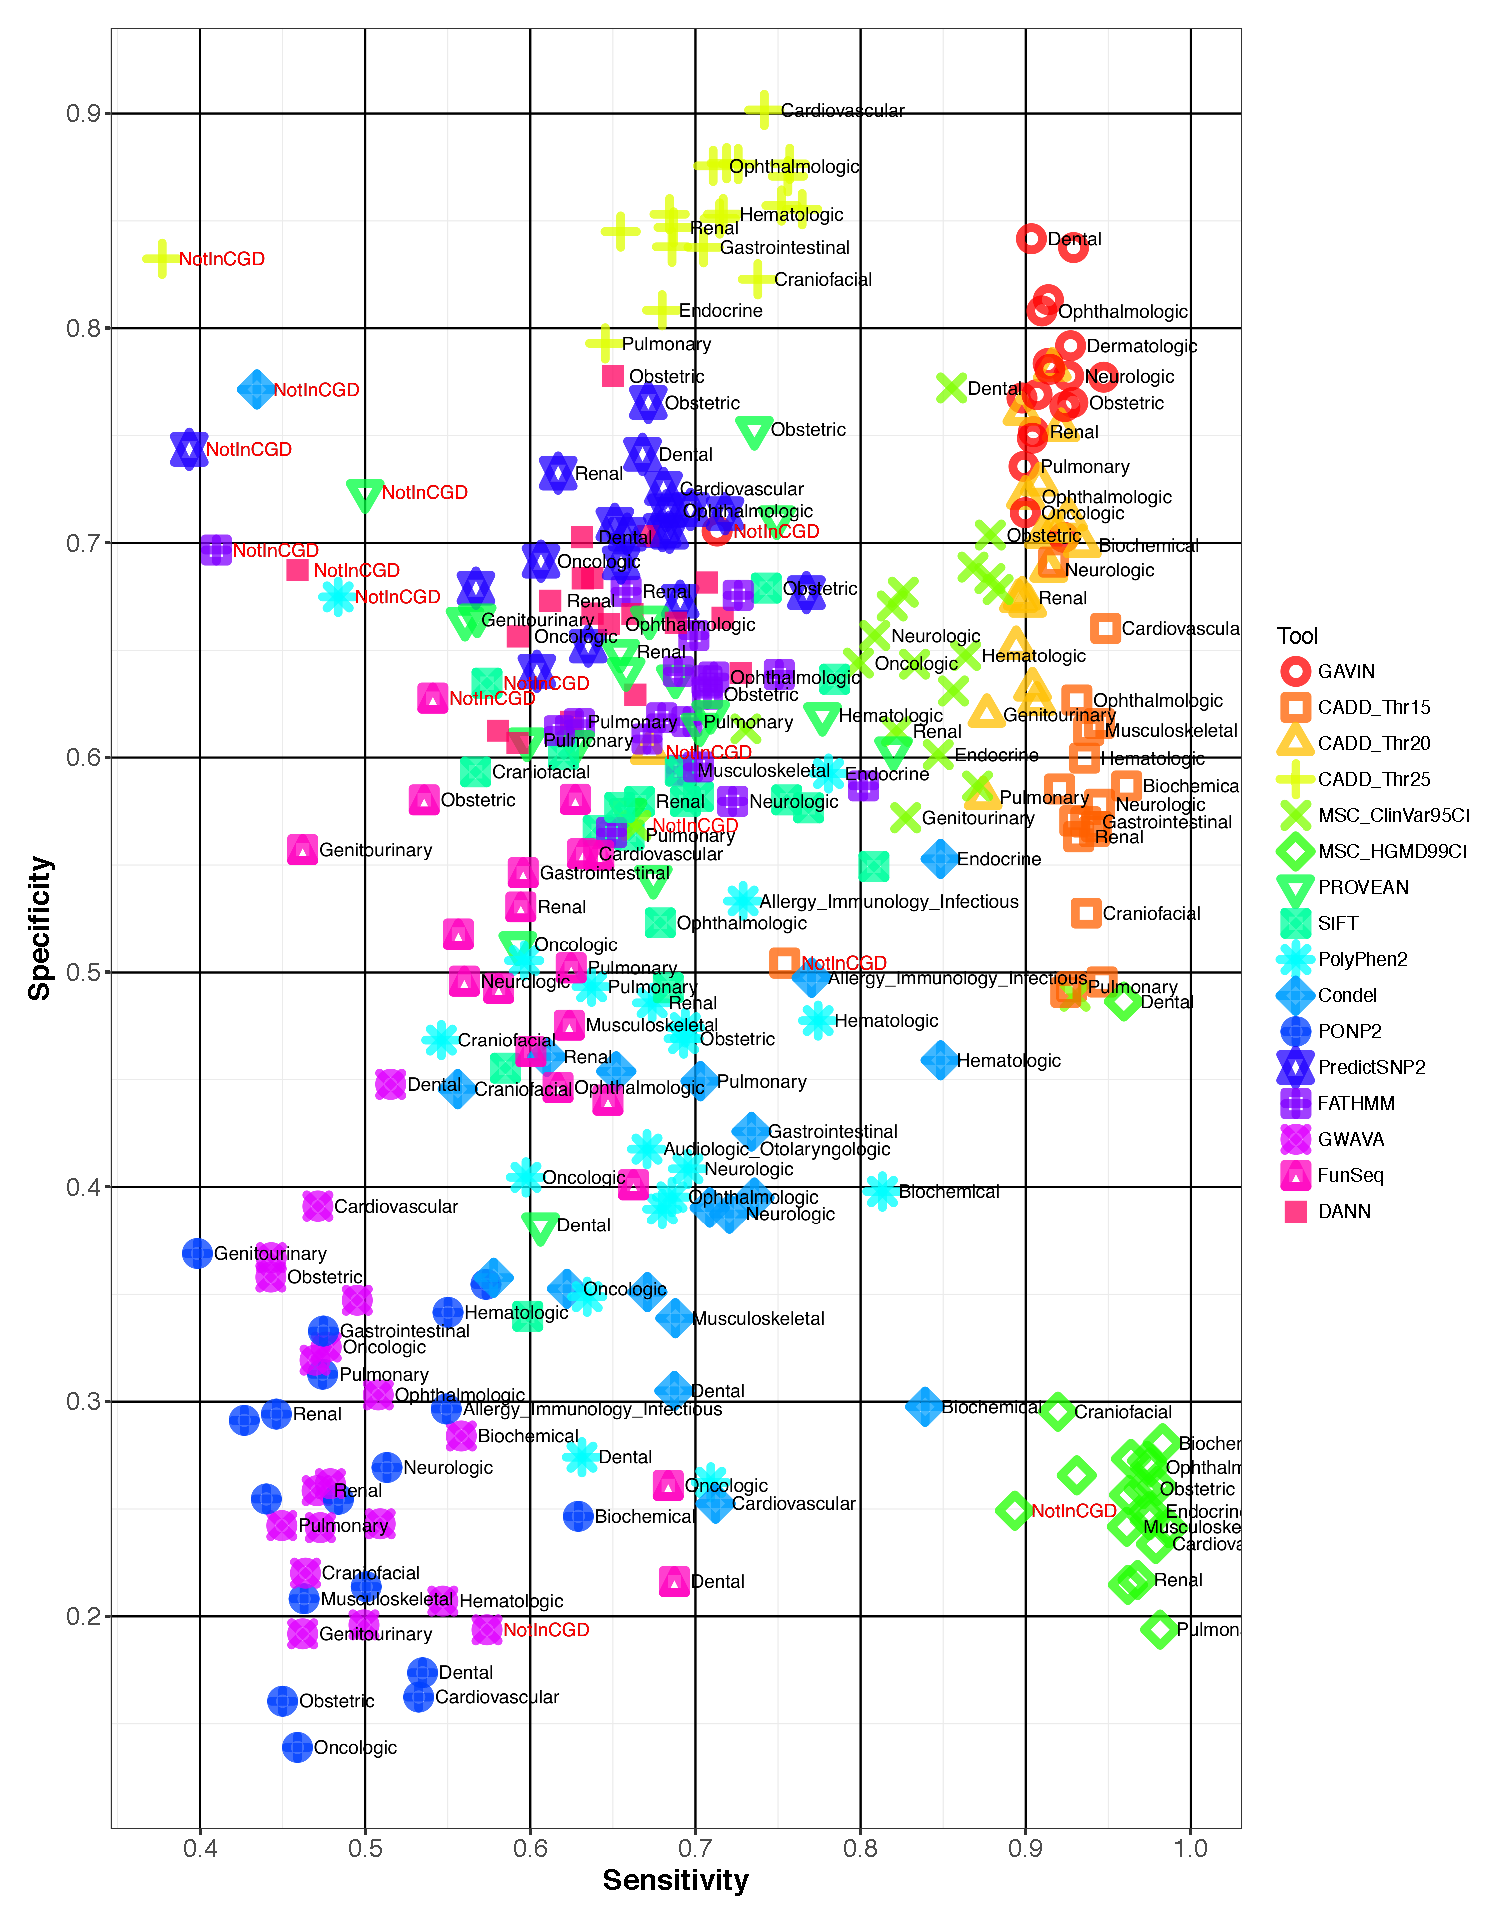
\includegraphics[width=1.0\linewidth]{img/gavin_performance}
	\caption[Performance of GAVIN and other tools]{Performance of GAVIN and other tools across different clinical gene sets. Prediction quality is measured as sensitivity and specificity, i.e. the fraction of pathogenic variants correctly identified and the fraction of misclassifications/non-classifications while doing so.}
	\label{fig:gavin_performance}
\end{figure}


\subsection{Added value of gene-specific calibration}
We then investigated the added value of using gene-specific thresholds on classification performance relative to using genome-wide thresholds.
We bootstrapped the performance on 10,000 random samples of 100 benign and 100 pathogenic variants.
These variants were drawn from the three groups of genes described in "\nameref{gavinmethods}": (1) genes for which CADD was significantly predictive for pathogenicity (\textsl{n} = 681); (2) genes where CADD was not significantly predictive (\textsl{n} = 732); and (3) genes with scarce variant data available for calibration (\textsl{n} = 774).
For each of these sets we compared the use of gene-specific CADD and MAF classification thresholds with that of genome-wide filtering rules.

We observed the highest accuracy on genes for which CADD had significant predictive value and for the gene-specific classification method (median accuracy = 87.5\%);
this was significantly higher than using the genome-wide method for these same genes (median accuracy = 84.5\%, Mann-Whitney U test \textsl{p} value $<$ 2.2e-16).
For genes for which CADD had less predictive value we found a lower overall performance, but still reached a significantly better result using the gene-specific approach (median accuracy = 84.5\% versus genome-wide 82.5\%, \textsl{p} value $<$ 2.2e-16).
Lastly, the worst performance was seen for variants in genes with scarce training data available.
The gene-specific performance, however, was still significantly better than using genome-wide thresholds (median accuracy = 82.5\% and 80.5\% respectively, \textsl{p} value = 2.2e-16).
See Figure \ref{fig:gavin_bootstrap}.


\begin{sidewaysfigure}
	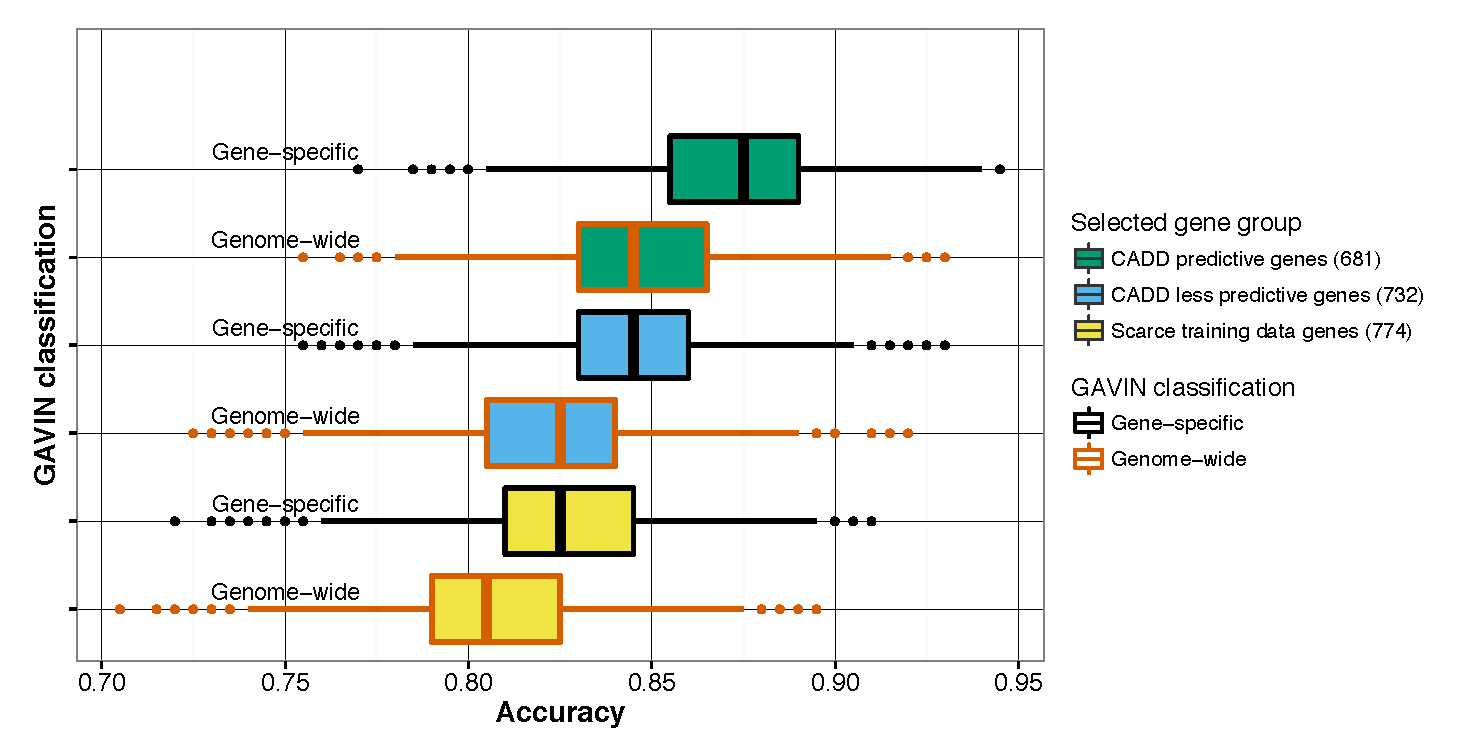
\includegraphics[width=1.0\linewidth]{img/gavin_bootstrap}
	\caption[Comparison of gene-specific thresholds]{Comparison of gene-specific classification thresholds with genome-wide fixed thresholds in three groups of genes: 737 genes for which CADD is predictive, 684 genes for which CADD is less predictive, and 766 genes with scarce training data. For each group, 10,000 sets of 100 benign and 100 pathogenic variants were randomly sampled and tested from the full set of 25,765 variants and accuracy was calculated for gene-specific and genome-wide CADD and MAF thresholds.}
	\label{fig:gavin_bootstrap}
\end{sidewaysfigure}


\section{Discussion}

We have developed GAVIN, a method for automated variant classification using gene-specific calibration of classification thresholds for benign and pathogenic variants.

Our results show that GAVIN is a powerful classifier with consistently high performance in clinically relevant genes.
The robustness of our method arises from a calibration strategy that first corrects for calibration bias between benign and pathogenic variants, in terms of consequence and rarity, before calculating the classification thresholds.
A comprehensive benchmark demonstrates a unique combination of high sensitivity ($>$90\%) and high specificity ($>$70\%) for variants in genes related to different organ systems.
This is a significant improvement over existing tools that tend to achieve either a high sensitivity (MSC, CADD at lower thresholds) or a high specificity (PredictSNP2, CADD at higher thresholds).
A high sensitivity is crucial for clinical interpretation because pathogenic variants should not be falsely discarded.
In addition, having a higher specificity means that the results will be far less "polluted" with false positives and thus less risk of patients being given a wrong molecular diagnosis.
GAVIN decreases false positives by 10-20\% compared to using CADD for the same purpose, thereby reducing interpretation time.
The difference between using a high and low performance method can be dramatic in practice.
In a hypothetical example, GAVIN would make downstream variant interpretation twice as effective as a low performance method, with more sensitive detection of pathogenic variants (see Table \ref{table:estimateofimpact}).


\begin{table}
\begin{tabulary}{\linewidth}{L|L|L|L|}
  Hypothetical data set & \textsl{90\% sensitive method} & \textsl{70\% sensitive method} \\
  100 benign variants & 9 pathogenic found & 7 pathogenic found \\
  10 pathogenic variants & 1 pathogenic missed & 3 pathogenic missed \\
  \hline
  \textsl{80\% specific method} & 9+20 = 29 variants to interpret & 7+20 = 27 variants to interpret \\
  80 benign found, 20 benign missed & 9/29 = 31\% positive predictive value & 7/27 = 26\% positive predictive value \\
  \hline
  \textsl{60\% specific method} & 9+40 = 49 variants to interpret & 7 + 40 = 47 variants to interpret \\
  60 benign found, 40 benign missed & 9/49 = 18\% positive predictive value & 7/47 = 15\% positive predictive value \\
  \hline
\end{tabulary}
\caption[Estimate of impact in clinical diagnostics]{Estimate of the practical impact in clinical diagnostics of using methods of different sensitivity and specificity on a data set with 100 benign and 10 pathogenic variants.}
\label{table:estimateofimpact}
\end{table}


Even though an optimal combination of sensitivity and specificity may be favorable in general terms, there may still be a need for tools that perform differently.
The MSC gene-specific thresholds based on HGMD\cite{Stenson_2013} at 99\% confidence interval show a very high sensitivity (97.1\%), but at the expense of a very low specificity (25.7\%).
Such low specificity thresholds will pick up almost all the pathogenic variants with scores exceeding gene thresholds.
This allows safe removal ($<$3\% error) of benign variants that fall below these thresholds, which was their authors’ aim.
However, this tool cannot detect pathogenic variants due its low specificity.
Other tools, such as PON-P2, may show a relatively low performance, but not necessarily because of true errors.
Such tools may simply be very ‘picky’ and only return a classification when the verdict carries high confidence.
If we ignore the variants that PON-P2 did not classify (52\% of total benchmark variants) and only consider how many of the variants that it did classify were correct, we find a positive predictive value of 96\% and a negative predictive value of 94\%.
Thus, while this tool might not be useful for exome screening because too many pathogenic variants would be lost, it can still be an excellent choice for further investigation of interesting variants.
We would therefore emphasize that appropriate tools should be selected depending on the question or analysis protocol used and by taking their strengths and weaknesses into account.

Not surprisingly, we could confirm that the use of gene-specific thresholds instead of genome-wide thresholds led to a consistent and significant improvement of classification performance.
This shows the added value of our strategy.
Overall performance was slightly lower in genes for which CADD has limited predictive value and even lower in genes with few "gold standard" pathogenicity data available.
Evaluating variants in uncharacterized genes is rare in clinical diagnostics, although it may occur when exome sequencing is aimed at solving complex phenotypes or undiagnosed cases.
Nevertheless, GAVIN is likely to improve continuously in an increasing number of genes, propelled by the speed at which pathogenic variants are now being reported.
The results of this paper are based on the ClinVar release of November 2015 and comprise 2,525 informative gene calibrations, i.e. thresholds for CADD, impact, MAF or a combination thereof.
When we calibrate on the September 2016 ClinVar release, we obtain more informative gene calibrations (2,770) with stable gene CADD thresholds (mean pathogenic difference of 0.1\%, mean benign difference of 1.1\%) and a slight drop in pathogenic MAF (0.00426 to 0.00346).
Using these newer calibrations, the benchmark performance of GAVIN increases to 91.7\% sensitivity (up from 91.4\%) and 78.2\% specificity (up from 76.9\%).
If this trend continues and (2770-2525)/10 = 24.5 genes per month are added, we estimate that calibrating all disease genes in CGD (3,316 per Sept. 2016) will take another (3316-2770)/24.5/12 = 1.86 $\approx$ 2 years.

With GAVIN, we were also able to demonstrate the residual power of CADD scores as a predictor for pathogenicity on a gene-by-gene basis, revealing that the scores are informative for many genes (these results can be accessed at \url{http://molgenis.org/gavin}).
There are several possible explanations for potential non-informativity of CADD scores.
It may have bias towards the in silico tools and sources it was trained on, limiting their predictiveness for certain genomic regions or disease mechanisms\cite{Mather_2016}.
Furthermore, calibration of pathogenic variants could be difficult in genes with high damage tolerance, i.e. having many missense or loss-of-function mutations\cite{Itan_2015}.
In addition, calibration may be impaired by false input signals, such as an incorrect pathogenic classification in ClinVar or inclusion of disease cohorts in large databases such as ExAC could misrepresent allele frequencies\cite{Song_2015}.
Lastly, pathogenic variants could have a low penetrance or their effect mitigated by genetic modifiers, causing high deleteriousness to be tolerated in the general population against expectations\cite{Cooper_2013}.

The field of clinical genomics is now moving towards interpretation of non-coding disease variants (NCVs) identified by WGS \cite{Zhang_2015}.
A number of recently introduced metrics, including EIGEN\cite{Ionita_Laza_2016}, FATHMM-MKL, DeepSEA\cite{Zhou_2015}, and GWAVA, specialize in predicting the functional effects of non-coding sequence variation.
When a pathogenic NCV reference set of reasonable quantity becomes available, a calibration strategy as described here will be essential to be able to use these metrics effectively in whole-genome diagnostics.


\section{Conclusions}

GAVIN provides an automated decision-support protocol for classifying variants, which will continue to improve in scope and precision as more data is publicly shared by genome diagnostic laboratories.
Our approach bridges the gap between estimates of genome-wide and population-wide variant pathogenicity and contributes to their practical usefulness for interpreting clinical variants in specific patient populations.
Databases such as ClinVar contain a wealth of implicit rules now used manually by human experts to classify variants.
Rules on minor allele frequencies, estimated effect impact and CADD scores are deduced and employed by GAVIN to classify variants that have not been seen before.

We envision GAVIN accelerating NGS diagnostics and becoming particularly beneficial as a powerful (clinical) exome screening tool.
It can be used to quickly and effectively detect over 90\% of pathogenic variants in a given data set and to present these results with an unprecedented small number of false positives.
It may especially serve laboratories that lack the resources necessary to perform reliable and large-scale manual variant interpretation for their patients and spur the development of more advanced gene-specific classification methods.
We provide GAVIN as an online MOLGENIS\cite{Swertz_2010a} web service to browse gene calibration results and annotate VCF files and as a commandline executable including open source code for use in bioinformatic pipelines.
GAVIN can be found at \url{http://molgenis.org/gavin}.


\section{Methods}
\label{gavinmethods}

\subsection{Calibration of gene-specific thresholds}
We downloaded ClinVar (variant\_summary.txt.gz from ClinVar FTP, last modified date: 05/11/15) and selected GRCh37 variants that contained the word “pathogenic” in their clinical significance.
These variants were matched against the ClinVar VCF release (clinvar.vcf.gz, last modified date: 01/10/15) using RS (Reference SNP) identifiers in order to resolve missing indel notations.
On the resulting VCF, we ran SnpEff version 4.1 L with these settings: hg19 -noStats -noLog -lof -canon -ud 0.
As a benign reference set, we selected variants from ExAC (release 0.3, all sites) from the same genic regions with +/- 100 bases of padding on each side to capture more variants residing on the same exon.
We first determined the thresholds for gene-specific pathogenic allele frequency by taking the ExAC allele frequency of each pathogenic variant, or assigning zero if the variant was not present in ExAC, and calculating the 95th percentile value per gene using the R7 method from Apache Commons Math version 3.5.
We filtered the set of benign variants with this threshold to retain only variants that were rare enough to fall into the pathogenic frequency range.

Following this step, the pathogenic impact distribution was calculated as the relative proportion of the generalized effect impact categories, as annotated by SnpEff on the pathogenic variants.
The same calculation was performed on the benign variants uniquely present in ExaC.
To facilitate this, we annotated ExAC with SnpEff (4.1 L, same settings as above) to get the same impact, transcript and gene nomenclature as our ClinVar set.
Overlapping genes were not an issue because SnpEff variant annotations include the gene symbol to which an estimated impact is applicable and subsequently only those matching impacts were considered.
The benign variants were subsequently downsized to match the impact distribution of the pathogenic variants.

For instance, in the case of 407 pathogenic MYH7 variants, we found a pathogenic allele frequency threshold of 4.942e-5, and an impact distribution of 5.41\% HIGH, 77.4\% MODERATE, 17.2\% LOW and 0\% MODIFIER.
We defined a matching set of benign variants by retrieving 1,799 MYH7 variants from ExAC (impact distribution: 2\% HIGH, 23.59\% MODERATE, 32.59\% LOW, 41.82\% MODIFIER), from which we excluded known ClinVar pathogenic variants (\textsl{n} = 99), variants above the AF threshold (\textsl{n} = 246), and removed interspersed variants using a non-random ‘step over’ algorithm until the impact distribution was equalized (\textsl{n} = 960).
We thus reached an equalized benign set of 494 variants, having an impact distribution of 5.47\% HIGH, 77.33\% MODERATE, 17.21\% LOW and 0\% MODIFIER).

We then obtained the CADD scores for all variants and tested whether there was a significant difference in scores between the sets of pathogenic and benign variants for each gene, using a Mann-Whitney U test.
Per gene we determined the mean CADD score for each group and also the 95th percentile sensitivity threshold (detection of most pathogenic variants while accepting false positives) and 95th percentile specificity threshold (detection of most benign variants while accepting false negatives), using the Percentile R7 function.
All statistics were done with Apache Commons Math version 3.5.
This calibration process was repeated for 3,237 genes, resulting in 2,525 genes for which we learned classification rules involving pathogenic variant MAF, effect impact distribution, CADD score thresholds, or a combination thereof.

On average, CADD scores were informative of pathogenicity.
The mean benign variant CADD score across all genes was 23.08, while the mean pathogenic variant CADD score was 28.44, a mean difference of 5.36 ($\sigma$ = 4.80).
Of 3,237 genes that underwent the calibration process, we found 681 “CADD predictive” genes that had a significantly higher CADD score for pathogenic variants than for benign variants (Mann-Whitney U test, \textsl{p} value $<$0.05).
Interestingly, we also found 732 “CADD less predictive” genes, for which there was no proven difference between benign and pathogenic variants (\textsl{p} value $>$0.05 despite having $\geq$ 5 pathogenic and $\geq$ 5 benign variants in the gene).
For 774 genes there was very little calibration data available ($<$5 pathogenic or $<$5 benign variants), resulting in no significant difference (\textsl{p} value $>$0.05) between CADD scores of pathogenic and benign variants.
We also found 159 genes for which effect impact alone was predictive, meaning that a certain impact category was unique for pathogenic variants compared to benign variants.
For instance, if we observe HIGH impact pathogenic variants (frame shift, stopgain, etc.) for a given gene, whereas benign variants only reach MODERATE impact (missense, inframe insertion, etc.), we use this criterion as a direct classifier.
No further CADD calibration was performed on these genes.
In summary, the total set of 3,237 genes comprises 681 “CADD predictive” genes + 732 “CADD less predictive” genes + 774 “little calibration data” genes + 159 “impact predictive” + 178 genes with only pathogenic MAF calibrated + 712 genes without calibration due to less than 2 ClinVar or ExAC variants available + 1 artifact where population CADD was greater than pathogenic CADD.
See Additional file 1: Table S1 for details.

\subsection{Variant sets for benchmarking}
We obtained six variant sets that had been classified by human experts.
These data sets were used to benchmark the in silico variant pathogenicity prediction tools mentioned in this paper.
Variants from the original sets may sometimes be lost due to conversion of cDNA/HGVS notation to VCF.

The VariBench protein tolerance data set 7 (\url{http://structure.bmc.lu.se/VariBench/}) contains disease-causing missense variations from the PhenCode\cite{Giardine_2007} database, IDbases\cite{Piiril__2006}, and 18 individual LSDBs\cite{Nair_2012}.
The training set we used contained 17,490 variants, of which 11,347 were benign and 6,143 pathogenic.
The test set contained 1,887 variants, of which 1,377 were benign and 510 pathogenic.
We used both the training set and test set as benchmarking sets.

The MutationTaster2\cite{Schwarz_2014} test set contains known disease mutations from HGMD\cite{Stenson_2013} Professional and putatively harmless polymorphisms from 1000 Genomes.
It is available at \url{http://www.mutationtaster.org/info/Comparison_20130328_with_results_ClinVar.html}.
This set contains 1,355 variants, of which 1,194 are benign and 161 pathogenic.

We selected 1,688 pathogenic variants from ClinVar that were added between November 2015 and February 2016 as an additional benchmarking set, since our method was based on the November 2015 release of ClinVar.
We supplemented this set with a random selection of 1,668 benign variants from ClinVar, yielding a total of 3,356 variants.

We obtained an in-house list of 2,359 variants that had been classified by molecular and clinical geneticists at the University Medical Center Groningen.
These variants belong to patients seen in the context of various disorders: cardiomyopathies, epilepsy, dystonia, preconception carrier screening, and dermatology.
Variants were analyzed according to Dutch medical center guidelines\cite{ACGN} for variant interpretation, using Cartagenia Bench Lab\textsuperscript{TM} (Agilent Technologies) and Alamut\textsuperscript{®} software (Interactive Biosoftware) by evaluating in-house databases, known population databases (1000G\cite{Auton_2015}, ExAC, ESP6500 at \url{http://evs.gs.washington.edu/EVS/}, GoNL\cite{Francioli_2014}), functional effect and literature searches.
Any ClinVar variants included in the November 2015 release were removed from this set to prevent circular reasoning, resulting in a total of 1,512 variants, with 1,176 benign/likely benign (merged as Benign), 162 VUS, and 174 pathogenic/likely pathogenic (merged as Pathogenic).

From the UMCG diagnostics laboratory we also obtained a list of 607 variants seen in the context of familial cancers.
These were interpreted by a medical doctor according to ACMG guidelines\cite{Richards_2015}.
We removed any ClinVar variants (November 2015 release), resulting in 395 variants, with 301 benign/likely benign (merged as Benign), 68 VUS and 26 likely pathogenic/pathogenic (merged as Pathogenic).

\subsection{Variant data processing and preparation}
We used Ensembl VEP (\url{http://grch37.ensembl.org/Homo_sapiens/Tools/VEP/}) to convert cDNA/HGVS notations to VCF format.
Newly introduced N-notated reference bases were replaced with the appropriate GRCh37 base, and alleles were trimmed where needed (e.g. “TA/TTA” to “T/TT”).
We annotated with SnpEff (version 4.2) using the following settings: hg19 -noStats -noLog -lof -canon -ud 0.
CADD scores (version 1.3) were added by running the variants through the CADD webservice (available at \url{http://cadd.gs.washington.edu/score}).
ExAC (release 0.3) allele frequencies were added with MOLGENIS annotator (release 1.16.2).
We also merged all benchmarking sets into a combined file with 25,995 variants (of which 25,765 classified as benign, likely benign, likely pathogenic or pathogenic) for submission to various online in silico prediction tools.

\subsection{Execution of in silico predictors}
The combined set of 25,765 variants was classified by the in silico variant pathogenicity predictors (MSC, CADD, SIFT, PolyPhen2, PROVEAN, Condel, PON-P2, PredictSNP2, FATHMM, GWAVA, FunSeq, DANN).
The output of each tool was loaded into a program that compared the observed output to the expected classification and which then calculated performance metrics such as sensitivity and specificity.
The tools that we evaluated and the web addresses used can be found in Table \ref{table:tool_urls}.
We executed PROVEAN and SIFT, for which the output was reduced by retaining the following columns: “INPUT”, “PROVEAN PREDICTION (cut-off = -2.5)” and “SIFT PREDICTION (cut-off = 0.05)”.
For PONP-2, the output was left as-is.
The Mutation Significance Cutoff (MSC) thresholds are configurable; we downloaded the ClinVar-based thresholds for CADD 1.3 at 95\% confidence interval, comparable to our method, as well as HGMD-based thresholds at 99\% confidence interval, the default setting.
Variants below the gene-specific thresholds were considered benign, and above the threshold pathogenic.
Following the suggestion of the CADD authors, scores of variants below a threshold of 15 were considered benign, above this threshold pathogenic.
We also tested CADD thresholds 20 and 25 for comparison.
The output of Condel was reduced by retaining the following columns: “CHR”, ”START”, ”SYMBOL”, ”REF”, ”ALT”, ”MA”, ”FATHMM”, ”CONDEL”, ”CONDEL\_LABEL”.
After running PolyPhen2, its output was reduced by retaining the positional information (“chr2:220285283|CG”) and the “prediction” column.
Finally, we executed PredictSNP2, which contains the output from multiple tools.
From the output VCF, we used the INFO fields “PSNPE”, “FATE”, “GWAVAE”, “DANNE” and “FUNE” for the pathogenicity estimation outcomes according to the PredictSNP protocol for PredictSNP2 consensus, FATHMM, GWAVA, DANN and FunSeq, respectively.


\begin{table}
\begin{tabulary}{\linewidth}{LL}
  Tool & Used via web address \\
  \hline
  \rule{0pt}{2.5ex}MSC & \url{http://pec630.rockefeller.edu/MSC/} \\
  \rule{0pt}{2.5ex}CADD & \url{http://cadd.gs.washington.edu/} \\
  \rule{0pt}{2.5ex}SIFT & \url{http://provean.jcvi.org/index.php} \\
  \rule{0pt}{2.5ex}PolyPhen2 & \url{http://genetics.bwh.harvard.edu/pph2/} \\
  \rule{0pt}{2.5ex}PROVEAN & \url{http://provean.jcvi.org/index.php} \\
  \rule{0pt}{2.5ex}Condel & \url{http://bg.upf.edu/fannsdb/query/condel} \\
  \rule{0pt}{2.5ex}PON-P2 & \url{http://structure.bmc.lu.se/PON-P2/} \\
  \rule{0pt}{2.5ex}PredictSNP2 & {\footnotesize\url{http://loschmidt.chemi.muni.cz/predictsnp2/}} \\
  \rule{0pt}{2.5ex}FATHMM & {\footnotesize\url{http://loschmidt.chemi.muni.cz/predictsnp2/}} \\
  \rule{0pt}{2.5ex}GWAVA & {\footnotesize\url{http://loschmidt.chemi.muni.cz/predictsnp2/}} \\
  \rule{0pt}{2.5ex}FunSeq & {\footnotesize\url{http://loschmidt.chemi.muni.cz/predictsnp2/}} \\
  \rule{0pt}{2.5ex}DANN & {\footnotesize\url{http://loschmidt.chemi.muni.cz/predictsnp2/}} \\
  \hline
\end{tabulary}
\caption[Tools used to evaluate our benchmark variant set]{The tools used to evaluate our benchmark variant set and the web addresses used through which they were accessed.}
\label{table:tool_urls}
\end{table}


\subsection[Stratification of variants using ClinGenDatab.]{Stratification of variants using Clinical Genomics Database}
We downloaded Clinical Genomics Database (CGD; the .tsv.gz version on 1 June 2016 from \url{http://research.nhgri.nih.gov/CGD/download/}).
A Java program evaluated each variant in the full set of 25,765 variants and retrieved their associate gene symbols as annotated by SnpEff.
We matched the gene symbols to the genes present in CGD and retrieved the corresponding physical manifestation categories.
Variants were then written out to separate files for each manifestation category (cardiovascular, craniofacial, renal, etc.).
This means a variant may be output into multiple files if its gene was linked to multiple manifestation categories.
However, we did prevent variants from being written out twice to the same file in the case of overlapping genes in the same manifestation categories.
We output a variant into the “NotInCGD” file only if it was not located in any gene present in CGD.

\subsection{Implementation}
GAVIN was implemented using Java 1.8 and MOLGENIS\cite{Swertz_2010a} 1.21 (\url{http://molgenis.org}).
The calibration method is agnostic of the meaning of pathogenic or benign, resulting in thresholds that have balanced sensitivity and specificity.
In our diagnostics practice, sensitivity is valued over specificity.
We therefore adjusted the CADD and MAF thresholds to shift the balance towards sensitivity at the cost of specificity.
We found a setting of 5 (adjustable in source code) achieved $>$90\% sensitivity and this setting was used to generate final thresholds.
The genome-wide classification thresholds based on CADD scores $<$ 15 for benign and $>$ 15 for pathogenic matched this high sensitivity.
The full table of gene-specific thresholds used can be found at \url{http://www.molgenis.org/gavin} (for latest release) or Additional file 1: Table S1.
They can be used to guide manual variant interpretation or be re-used in other tools.
Source code with tool implementation details can be found at \url{https://github.com/molgenis/gavin}.
All benchmarking, bootstrapping and plotting tools can be found in this repository, as well as all data processing and calibration programs.

\subsection{Binary classification metrics}
Prediction tools may classify variants as benign or pathogenic, but may also fail to reach a classification or classify a variant as VUS.
Because of these three outcome states, binary classification metrics must be used with caution.
We define sensitivity as the number of detected pathogenic variants (true positives) over the total number of pathogenic variants, which includes true positives, false negatives (pathogenic variants misclassified as benign), and pathogenic variants that were otherwise "missed", i.e. classified as VUS or not classified at all.
Therefore, Sensitivity = TruePositive/(TruePositive + FalseNegative + MissedPositive).
We applied the same definition for specificity and define it as: Specificity = TrueNegative/(TrueNegative + FalsePositive + MissedNegative).
Following this line, accuracy is then defined as (TruePositive + TrueNegative)/(TruePositive + TrueNegative + FalsePositive + FalseNegative + MissedPositive + MissedNegative).

\section*{Additional files}
\textbf{Additional file 1: Table S1.} GAVIN gene-specific thresholds used in the benchmark.
This table can be used to look up thresholds of individual genes and allow variant interpretation by following classification rules as indicated by the column names and provided explanation.
(XLSX 198 kb) [available online at \url{genomebiology.biomedcentral.com}]\\
\textbf{Additional file 2: Table S2.} Detailed overview of all benchmark results.
Each combination of tool and dataset is listed. We provide the raw counts of true positives (TP), true negatives (TN), false positives (FP), and false negatives (FN), as well as of pathogenic and benign variants that were "missed", i.e. not correctly identified as such.
From these numbers, we calculated the sensitivity and specificity.
(XLSX 58 kb) [available online at \url{genomebiology.biomedcentral.com}]\\
\textbf{Additional file 3: Table S3.} \textsl{Included in this chapter as Table \ref{table:estimateofimpact}}\\
\textbf{Additional file 4: Table S4.} \textsl{Included in this chapter as Table \ref{table:tool_urls}}

\section*{Acknowledgements}
We thank Jackie Senior, Kate McIntyre, and Diane Black for their editorial advice.
We thank the MOLGENIS team for their assistance with the software implementation and the GAVIN user interface: Bart Charbon, Fleur Kelpin, Mark de Haan, Erwin Winder, Tommy de Boer, Jonathan Jetten, Dennis Hendriksen, and Chao Pang.

\section*{Funding}
We thank BBMRI-NL for sponsoring the above software development via a voucher.
BBMRI-NL is a research infrastructure financed by the Netherlands Organization for Scientific Research (NWO), grant number 184.033.111.
We also thank NWO VIDI grant number 016.156.455.

\section*{Availability of data and material}
The datasets generated during and/or analysed during the current study are available in the GAVIN public GitHub repository, available at \url{https://github.com/molgenis/gavin}.
We have released citable DOI objects for the full source code of both GAVIN, available at \url{https://doi.org/10.5281/zenodo.155254} and its MOLGENIS dependency at \url{https://doi.org/10.5281/zenodo.155255}.

\section*{Authors’ contributions}
KV, EB, and MS conceived the method.
KV, EB, CD, BS, KA, LF, CW, RHS, RJS, and TK helped to fine-tune the method, accumulate relevant validation data, and evaluate the results.
KV and MS drafted the manuscript.
KV, EB, CD, BS, KA, AK, LF, FS, TK, CW, RHS, RJS, and MS edited and reviewed the manuscript.
All authors read and approved the final manuscript.

\section*{Competing interests}
The authors declare that they have no competing interests.

\section*{Consent for publication}
Not applicable.

\section*{Ethics approval and consent to participate}
The study was done in accordance with the regulations and ethical guidelines of the University Medical Center Groningen.
Specific ethical approval was not necessary because this study was conducted on aggregated, fully anonymized data.

\chapter[A bioinf. framework for downstream genome analysis]{A bioinformatics framework for flexible automation of downstream genome analysis}
\chaptermark{Bioinf. framework for genome analysis}
\label{chap:frameworkforgenomics}

{ \Large \leftwatermark{
\put(-67,-66.5){ 1 }
\put(-67,-91.5){ 2 }
\put(-67,-116.5){ 3 }
\put(-67,-141.5){ 4 }
\put(-67,-166.5){ 5 }
\put(-67,-191.5){ 6 }
\put(-76.5,-225){\includegraphics[scale=0.8]{img/thumbindex.eps}} \put(-67,-216.5){ {\color{white} 7 }}
\put(-67,-241.5){ 8 }
} \rightwatermark{
\put(350.5,-66.5){ 1 }
\put(350.5,-91.5){ 2 }
\put(350.5,-116.5){ 3 }
\put(350.5,-141.5){ 4 }
\put(350.5,-166.5){ 5 }
\put(350.5,-191.5){ 6 }
\put(346.5,-225){\includegraphics[scale=0.8]{img/thumbindex.eps}} \put(350.5,-216.5){ {\color{white} 7 }}
\put(350.5,-241.5){ 8 }
}}

\hfill \textsl{unpublished}

\newpage

\noindent
K. Joeri van der Velde\textsuperscript{1,2}, Lennart F. Johansson\textsuperscript{2}, Ellen Carbo\textsuperscript{3}, Bart Charbon\textsuperscript{1}, Martine Meems-Veldhuis\textsuperscript{2}, Dennis Hendriksen\textsuperscript{1}, Cleo C. van Diemen\textsuperscript{2}, Freerk van Dijk\textsuperscript{1,2}, Fleur Kelpin\textsuperscript{1}, Kristin M. Abbott\textsuperscript{2}, Birgit Sikkema-Raddatz\textsuperscript{2}, Richard J. Sinke\textsuperscript{2} and Morris A. Swertz\textsuperscript{1,2,*}\\

\noindent
1. University of Groningen, University Medical Center Groningen, Genomics Coordination Center, Groningen, The Netherlands\\
2. University of Groningen, University Medical Center Groningen, Department of Genetics, Groningen, The Netherlands\\
3. University Medical Center Utrecht, Department of Genetics, Utrecht, The Netherlands\\

\noindent
* To whom correspondence should be addressed.

\section*{Abstract}

With the popularity of next-generation sequencing rising, we expect thousands of individuals to soon have whole-genome profiling.
However,  implementation is a huge challenge for both genome research and diagnostic applications, with the primary roadblock not data acquisition or variant calling, but downstream interpretation.

Interpretation can be sped up using the huge amount of useful information collected by laboratories, public databases and biobanks. Unfortunately, for now, all these sources of useful data cannot be easily integrated and explored in unison. Further, while many innovative analysis methods emerge from research on a regular basis, a lack of standardization makes it difficult to adopt, share, compare and validate them in practice.

Here we report a lightweight framework for genome interpretation pipelines that aims to enable rapid implementation and adaptation of analysis protocols that integrate reference annotation data (e.g. ClinVar, ExAC, GoNL), run best-practice analysis tools (e.g. VAAST or GAVIN), capture their outputs in a standardized way using a new VCF extension, and use those outputs to generate informative, customizable reports for human interpretation.
Clear definitions of tools and standardization of outputs enable interoperability/flexibility and encourage members of the genomics community to jointly develop and reuse framework components in order to rapidly integrate new data and methods and develop and share new best practice protocols.
Standardized validation and benchmarking enables rapid testing and uptake of these developments.
We used MOLGENIS open source for its implementation but the framework can be readily added in other software.

Implementation of this framework in a genome diagnostic setting shows that we can successfully translate the latest knowledge and methods to medical practice.
However, we also envision its usage for different types of genomic studies because the framework is straightforward and offers advantages in terms of storing and sharing results.
Software downloads, manuals and source code can be found at \url{www.molgenis.org/genomics}.


\section{Introduction}

Sequencing of DNA and RNA has become pivotal in modern life science research, and we can now exploit our understanding of the genome to develop molecular diagnostic tests for many disorders.
However, when it comes to making more discoveries in research, there is still a need for better data integration\cite{Ritchie_2015} in order to discover new disease genes.
At the same time, in genome diagnostics, an increasing number of patients expect a reliable molecular diagnosis based on their complete genome\cite{Berg_2011} while diagnostic yield is still highly variable\cite{Wang_2014, Mart_nez_2016, Daoud_2016, Yubero_2016}.

To improve the situation, we can utilize a rapidly growing list of relevant methods, data and knowledge tools. Unfortunately, sharing and uptake of these new analysis resources is difficult because it takes considerable effort to investigate, adapt and validate them into diagnostic or research protocols.
This is partly because the quality and reusability of academic software remains low\cite{Prins_2015} while commercial software prefers to incorporate widely used methods that lag behind innovation. As a result, institutes develop their own interpretation strategies, with varying degrees of success\cite{Brownstein_2014}, to keep up with a quickly evolving field.

To encourage sharing and incorporation of community-built and commercial tools they should be easy to adopt into the interpretation workflows used in practice.
The first step to achieving this is to agree on the definitions of each processing step instead of focusing on implementations.
This has already happened for NGS variant calling pipelines\cite{Weiss_2013}, which are often composed of multiple commandline tools that are loosely connected by scripts and intermediate output files.
In NGS variant calling, steps such as aligning sequenced reads and variant calling are carried out by tools such as BWA, Samtools and GATK.
In this process, they use standard file formats FASTA/FASTQ, BAM/SAM and VCF (Variant Call Format).
This separation allows tools to be interchanged and optimized as a distinct unit of functionality in a bigger pipeline, driving innovations like Sambamba\cite{Tarasov_2015}, which is specifically developed for high-performance filtering of BAM files.

To better serve both research and routine diagnostic needs, we now wished to expand our NGS pipelines further downstream with the same modularity for fast integration and exchange of genome analysis methods such as the recently published GAVIN tool\cite{van_der_Velde_2017}.
To facilitate this, we present here a framework for standardized genomic analysis with interchangeable components.
It includes a new intermediate VCF-based format to capture relevant findings as the basis for interoperability between the tools in the pipeline, a task for which there was no pre-existing solution. We have tested and validated this framework with an open source implementation for genome diagnostics including tools for variant annotation, interpretation and reporting.


\section{Results}

\subsection{Framework for downstream genome analysis}

We developed a variant analysis framework consisting of a number of intermediate files and tool roles (annotation, analysis, and reporting).
The intermediate files use the well-known VCF specification, with additional extensions to support interoperability between alternative tools that fulfill the same role.
A new VCF extension called rVCF (Report VCF) is used to describe variants of interest.

We implemented and validated the framework into an existing bioinformatics pipeline within UMCG clinical genome diagnostics laboratory using both existing and newly developed tools.
See Figure \ref{fig:frameworkforgenomics_overview} for an overview of the components and data flow within the framework.
Below we first describe the file formats and tool roles involved and then provide examples of the implementation, usage and results of the framework as applied to genome diagnostics.\\

\begin{sidewaysfigure*}
\centering
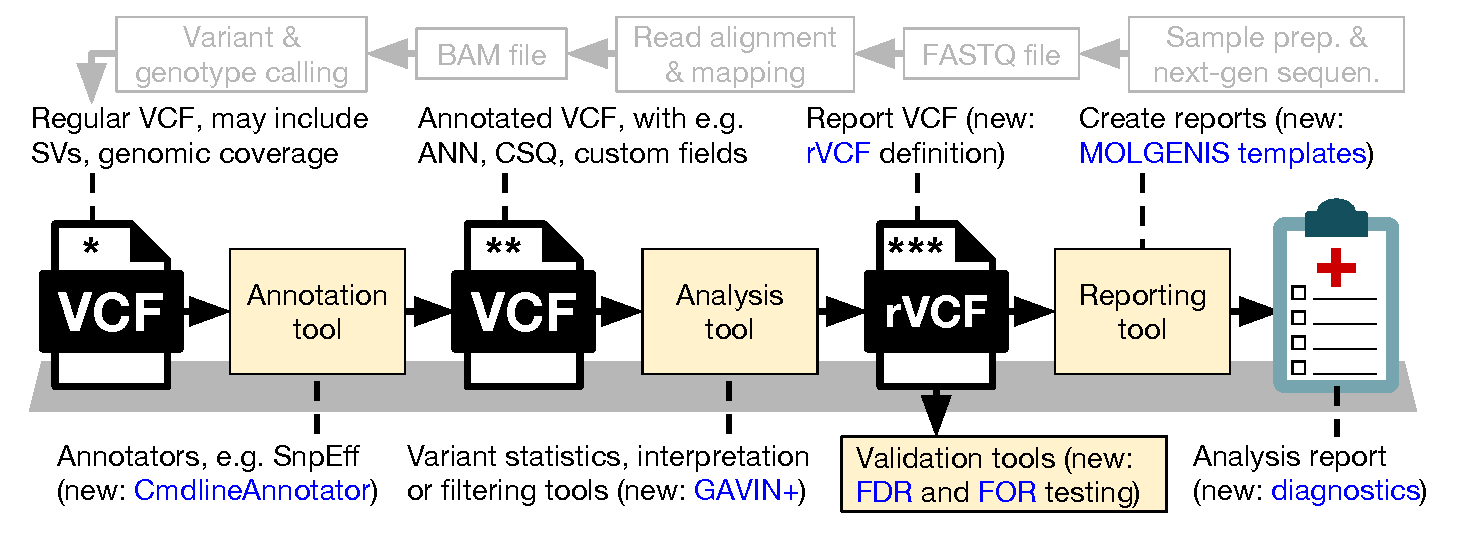
\includegraphics[width=1.0\linewidth]{img/frameworkforgenomics_overview}
\caption[Overview of the framework for automation]{Overview of the framework for adaptable automation of downstream genome analysis. New tools and formats developed for the genome diagnostic implementation of the framework are highlighted in blue. Upstream pipeline steps that are not part of the framework are shown in grey.}
\label{fig:frameworkforgenomics_overview}
\end{sidewaysfigure*}

\noindent We define the following intermediate files and tool roles: \\

\noindent\textbf{Regular VCF} files capture SNVs and small indels with the option to also capture genomic coverage and structural variants using existing definitions.
The VCF 4.2 standard\footnote{\url{https://samtools.github.io/hts-specs/VCFv4.2.pdf}} can describe any type of variation.
For genomic coverage, the gVCF\footnote{\url{https://software.broadinstitute.org/gatk/guide/article?id=4017}} extension may be used.\\

\noindent\textbf{Annotation tools} such as SnpEff\cite{Cingolani_2012}, Ensembl VEP\cite{McLaren_2010}, Jannovar\cite{J_ger_2014}, VarioWatch\cite{Cheng_2012} and CmdlineAnnotator (presented below).
These tools accept VCF files as input and add more contextual information per variant. \\

\noindent\textbf{Annotated VCF} files contain the enrichment of variants with additional contextual information from population references, known disease genes/variants, in silico pathogenicity estimates, GWAS, pathways and more.
This is stored in a standardized way to ensure tool interoperability (i.e. steps can be changed without needing to rewrite the pipeline).
We reuse existing field definitions where possible, such as the SnpEff ANN field\footnote{\url{http://snpeff.sourceforge.net/VCFannotationformat_v1.0.pdf}} and Ensembl VEP CSQ field\footnote{\url{http://www.ensembl.org/info/docs/tools/vep/vep_formats.html}}.
In addition, we added fields such as CADD\_\-SCALED (for CADD scores) and EXAC\_\-AF (for ExAC allele frequencies) for more annotations.\\

\noindent\textbf{Analysis tools} such as GE\-MI\-NI\cite{Paila_2013}, In\-ter\-Var\cite{Li_2017}, VI\-KING\cite{Miller_2015}, KGG\-Seq\cite{Li_2012}, VAAST\cite{Kennedy_2014} and GA\-VIN+ (presented below).
These tools filter and query annotated VCFs to find candidate variants.
Ideally, these tools output their results in Report VCF which can be processed or visualized further by other tools. \\

\noindent\textbf{Report VCF} files store the outcome of a genome analysis, such as GWAS p-values or diagnostic interpretation.
This intermediate file format stores relevant findings in a computer-readable format to increase pipeline flexibility by disconnecting results from reporting (see Figure \ref{fig:frameworkforgenomics_rvcfapplications}).
We build upon the VCF format by defining a specific extension for results, abbreviated 'rVCF'.
This format is fully VCF-compliant but adds an extra INFO field named RLV (relevance) that ensures tool interoperability within this framework.
This field contains the explanation for why this variant was thought to be relevant for the question imposed on the original data.

The RLV field was developed with the following criteria in mind: it should (i) be broad enough to allow many types of uses (e.g. for diagnostics, genome research, population studies); (ii) be specific enough for the results captured to be informative, at least for our diagnostic use case; (iii) provide all necessary contextual information to explain why a variant is relevant for the question posed; (iv) be structured and simple enough to allow reports to be created in a straightforward way (e.g. by templating); and (v) not contain unnecessary fields that would bloat the specification beyond its intended purpose and make it harder to use.
See Table \ref{table:frameworkforgenomics_rvcffields} for a detailed breakdown of the fields in the rVCF specification and how they can be used for different use-cases.\\

\begin{figure*}
\centering
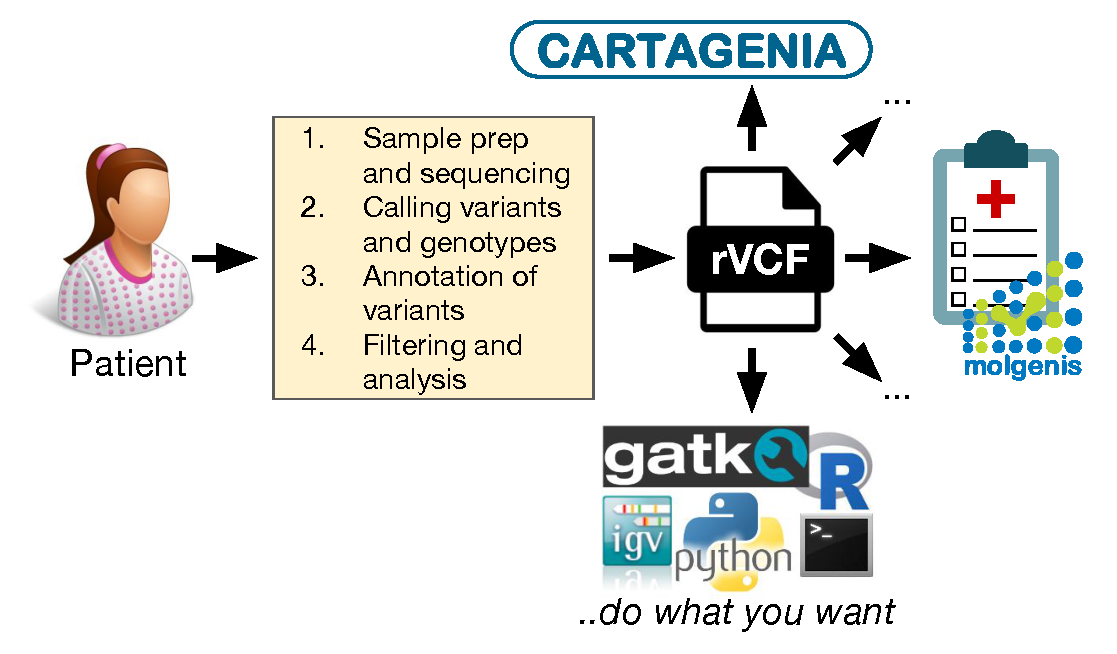
\includegraphics[width=1.0\linewidth]{img/frameworkforgenomics_rvcfapplications}
\caption[Applications of the rVCF format]{Creation and possible applications of the rVCF format. After the output has been generated by the analysis step, the results are stored in an rVCF file. This file can then be further analyzed or used to create a report. We have processed and visualized results in MOLGENIS\cite{Swertz_2010a} and Cartagenia Bench Lab\textsuperscript{TM} (Agilent Technologies), but any other tool or environment can be used including GATK\cite{Van_der_Auwera_2013}, Integrative Genomics Viewer\cite{Thorvaldsdottir_2012}, scripting languages and command line.}
\label{fig:frameworkforgenomics_rvcfapplications}
\end{figure*}

\begin{table*}
\scriptsize
\begin{tabulary}{\linewidth}{LL}
  \mbox{Field~~~~~~~~~~~~~~~~~~~~~~~~~~~~~~~~~~~~~~~~~~~~~~~~~~~~~~~~~~~~~~~~~~~~~~~~~~~~~~~~~~~~~~~~~~~} & Definition \\
  \hline
  \rule{0pt}{2.5ex}allele & The alternative allele in question, since VCF has multi-allelic sites \\
  \rule{0pt}{2.5ex}alleleFreq & Reference database minor allele frequencies, e.g. ExAC, GoNL or 1000G \\
  \rule{0pt}{2.5ex}gene & Gene name or identifier, e.g. HGNC symbol or MIM accession \\
  \rule{0pt}{2.5ex}FDR & Any pre-calculated FDR thresholds for this variant, gene or transcript \\
  \rule{0pt}{2.5ex}transcript & Transcript used, e.g. SnpEff canonical transcript \\
  \rule{0pt}{2.5ex}phenotype & Trait of disorder in question, e.g. trichotillomania, BMI or ethosuximide resistant \\
  \rule{0pt}{2.5ex}phenotypeInheritance & Mode of inheritance, e.g. dominant, recessive, additive \\
  \rule{0pt}{2.5ex}phenotypeOnset & Age of onset, e.g. pediatric, adult, L2-stage \\
  \rule{0pt}{2.5ex}phenotypeDetails & Extra phenotype info, e.g. treatment options or literature references \\
  \rule{0pt}{2.5ex}phenotypeGroup & Grouping of phenotypes, e.g. cardiovascular, neurological, oncological \\
  \rule{0pt}{2.5ex}$<many>$ sampleStatus & How this sample is potentially affected based on genotype and inheritance e.g. HOMZYG, AFFECTED, COMPOUND, DENOVO, CARRIER \\
  \rule{0pt}{2.5ex}$<many>$ samplePhenotype & The actual sample phenotype, taken from VCF 'SAMPLE' annotation field \\
  \rule{0pt}{2.5ex}$<many>$ sampleGenotype & Sample variant or marker genotypes with possibly quality or probability data \\
  \rule{0pt}{2.5ex}$<many>$ sampleGroup & Grouping of samples, e.g. case, control, EUR, AFR, infant, adult \\
  \rule{0pt}{2.5ex}variantSignificance & Type or value of variant significance, e.g. Reported pathogenic, Predicted pathogenic, pval 0.0035 \\
  \rule{0pt}{2.5ex}variantSignificanceSource & Tool or source used to discover this variant, e.g. your lab list, ClinVar, PolyPhen2, CADD, SIFT, GAVIN \\
  \rule{0pt}{2.5ex}variantSignificanceJustification & The reason why source thought this variant was interesting, or the criteria used by prediction tool \\
  \rule{0pt}{2.5ex}variantMultiGenic & Denote how this variant is potentially part of digenic or other complex forms of inheritance \\
  \rule{0pt}{2.5ex}variantGroup & Grouping of variants, e.g. suggestive, significant, iarc\_\-class\_\-5 \\
  \hline
\end{tabulary}
\caption[rVCF format specification]{rVCF format. Interoperability is ensured by standardizing interpretation information within the framework using a new 'RLV' field. Within this field, specific interpretation data can be described using the VCF standard INFO sub-field structure. Any sub-fields marked with $<many>$ may contain multiple values, each linked to specific sample identifiers. Multiple RLV values may be present to accommodate multi-allelic variants and overlapping gene annotations.}
\label{table:frameworkforgenomics_rvcffields}
\end{table*}

\noindent\textbf{Reporting tools} turn Report VCF into result overviews that can be read by human users and tailored to a specific audience.
A database system such as MOLGENIS, for example, can import, store, query and share genomic data and analysis results, then format it for diagnostics reporting from a diagnostics lab in a way that the clinical geneticist can use.
The system can be used to create analysis reports from the stored results.\\

\noindent\textbf{Analysis reports} are the final products of the downstream analysis.
They can be clinical patient reports for doctors or statistical genome-wide reports for researchers.
Multiple reports for different users and questions may be generated from an analysis, and within a report there is no limit on flexibility or interactivity, although use of single file documents with a simple and well-thought out graphical layout is encouraged.\\

\noindent\textbf{Validation tools} (automatically) test and evaluate pipeline results in a standardized way against a gold-standard data set.
Such validation is a precondition for diagnostics implementation.
Examples of possible validation tests include a false omission test to count how many expected hits were actually observed in the Report VCF output, a false discovery test to see how many unexpected hits were found, or a combination of the two.
These tests can be executed on individual level, on gene level, or across the whole genomes of many individuals simultaneously.
Validations of the pipeline are (automatically) performed whenever software versions or data sources have been updated.

\subsection{Implementation for genome diagnostics}

We used this framework to implement an automated downstream analysis and reporting pipeline for genome diagnostics.
Below we describe examples of annotation, analysis and reporting tools that are connected by using the standardized interpretation data format.

\subsubsection{Annotation tool: CmdlineAnnotator}

We implemented a high-performance tool that performs annotation tasks that enable variant enrichment.
It wraps common genomic annotation sources, such as ExAC\cite{Lek_2016}, 1000 Ge\-nomes\cite{Auton_2015}, Ge\-nome of the Ne\-ther\-lands\cite{Francioli_2014}, Clin\-Var\cite{Landrum_2015} and CADD\cite{Kircher_2014} in a standardized way. 
This enables us to quickly add and combine different annotation steps, which was one of our goals with this framework.
The tool, MOLGENIS CmdlineAnnotator, can be run on command line making it easy to script into typical bioinformatic pipelines, but we have also implemented a web interface for interactive use.
The tool requires no installation other than downloading an executable, and its use is straightforward.
MOLGENIS CmdlineAnnotator supports any valid VCF file, handles multi-allelic variants and can match equivalent variants even when their notation is different (see Methods and Materials).

\subsubsection{Analysis tool: GAVIN+}

We also created a new analysis tool to replace the analysis protocol we had used before.
GAVIN+ is a diagnostic interpretation tool that prioritizes DNA variants of potential clinical relevance in the genome.
It achieves this by using GAVIN\cite{van_der_Velde_2017}, a sensitive tool to predict pathogenic variants based on gene-specific CADD scores calibrated on ExAC, ClinVar and SnpEff.
In addition, GAVIN+ matches against candidates against known pathogenic variants in ClinVar but removes potential false positives with a GoNL/ExAC $>$5\% MAF.
The tool then queries the Clinical Genomics Database\cite{Solomon_2013} to find affected and carrier individuals depending on sample genotype and mode of inheritance.
For uncharacterized genes, the default heterozygous, compound heterozygous and homozygous states are assigned.
Depending on the input VCF, additional knowledge is automatically used.
This includes trio-aware sample filtering and genotype phasing to check validity of compound heterozygous hits, or reassigning status from, e.g., ‘homozygous by compound mutation’ back to ‘multiple hits on the same allele’.
Hemizygous genotypes for chromosome X and Y are also taken into consideration.
The tool even works on mitochondrial genotypes, albeit with limited references.
We run GAVIN+ as a command line runnable standalone tool that takes an annotated VCF file and returns a Report VCF file.

\subsubsection{Report VCF: novel format}

The Report VCF (rVCF) format is used to mark variants that may be of clinical interest.
The field that captures the clinical relevance, which is similar to SnpEff's ANN field, consists of a single string with multiple sub-fields separated by pipe symbols.
The values are described in the VCF header and include the alternative allele in question, gene, and transcript (just as in ANN), but rVCF also includes associated phenotype, inheritance mode, onset, genotype and affected/carrier status of samples, reason why this variant was relevant and according to whom.

There are currently 19 values within the RLV field, but in practice the notation is quite compact because unused sub-fields add only one character to the notation.
See Table \ref{table:frameworkforgenomics_rvcfdata} for examples of comparable VCF INFO field extensions for the same variant, including an example of the RLV field.

\begin{table*}
\begin{tabulary}{\linewidth}{LL}
  VCF INFO field & Data example \\
  \hline
  Consequence annotations from Ensembl VEP & CSQ=T $|$ 5\_\-prime\_\-UTR\_\-variant $|$ MODIFIER $|$ UROS $|$ ENSG00000188690 $|$ Transcript $|$ ENST00000368797 $|$ protein\_\-coding $|$ 1/10 $| | | |$ 7 $| | | | | | |$ -1 $| |$ HGNC $|$ 12592; \\
  ~ & ~ \\
  Functional annotations from SnpEff & ANN=T $|$ 5\_\-prime\_\-UTR\_\-variant $|$ MODIFIER $|$ UROS $|$ UROS $|$ transcript $|$ NM\_\-000375.2 $|$ Coding $|$ 1/10 $|$ c.-219C$>$A $| | | | |$ 6722 $|$; \\
  ~ & ~ \\
  Relevance annotations from GAVIN+ & RLV=T $|$ 0.0 $|$ UROS $|$ 0.0 0.011980830670926517 $|$ NM\_\-000375.2 $|$ Porphyria congenital erythropoietic $|$ RECESSIVE $|$ Pediatric $| | |$ DNA7654321:CARRIER $| |$ DNA7654321:0s1 $| |$ Reported pathogenic $|$ ClinVar $|$ NM\_\-000375.2(UROS):c.-219C$>$A UROS Pathogenic $| |$; \\
  \hline
\end{tabulary}
\caption[Examples of VCF INFO field definitions]{Examples of VCF INFO field definitions. The VEP consequence and SnpEff annotation fields describe the functional effects of a variant on genes and transcripts at its locus. The relevance field denotes why this particular variant and effect was included in the analysis result, such as screening for candidates that may explain a clinical phenotype.}
\label{table:frameworkforgenomics_rvcfdata}
\end{table*}

Because all applicable sample genotypes in question are now stored in the RLV field,  information on the genotype used is left out of the rVCF file.
The data reduction achieved by selecting only variants of potential relevance is substantial, and turns out very relevant for usage in a health care setting.
For example, on a data set of samples from 69 patients that were sequenced for panel of 96 dystonia genes, we reduce 2,154 variants (6.3 megabyte, MB) to 63 variants (90 kilobyte, kB).
A patient exome of 108,004 variants (77 MB) was reduced to 449 variants (625 kB), and a combined VCF with 282 exomes of 790,297 variants (7.3 GB) was reduced to 19,572 variants (17 MB).
In research one might still want to retain all data, therefore we developed a helper tool to merge the rVCF files back into the full list of variants and genotypes in the original VCF file, which provides more flexibility for how the format can be used.
Another helper tool can split the compound RLV field into many separate info fields for ease of import and filtering in other tools.

\subsubsection{Reporting tool: patient report for genome diagnostics}

We have implemented a report generator to visualize the information contained within rVCF using the MOLGENIS web database, although interested readers can easily write their own.
The rVCF files can be uploaded and stored in the database just like any other VCF file.
After importing, the genomic data can be browsed, queried, visualized and filtered using standard MOLGENIS UI components in the Data Explorer.
In addition, users can generate reports based on a simple template language (FreeMarker) and use R, Python or JavaScript and web services to make very interactive reports.
These templates can be uploaded, customized, changed, and reused within the database itself.

We have defined a patient report template that transforms the data into an overview showing the main findings of potential clinical relevance.
This report ranks the variants by importance for medical interpretation based on the evidence from the data and how well genes and variants are clinically characterized\cite{McLaughlin_2014}.
Users can apply a number of post-filters within the report if needed.
For instance, they may wish to exclude or include certain genes, e.g. those for late-onset disorders in the case of a young patient, or adjust the variant MAF inclusion threshold.
See Figure \ref{fig:frameworkforgenomics_patientreport} for an example of this report.

\begin{sidewaysfigure*}
\centering
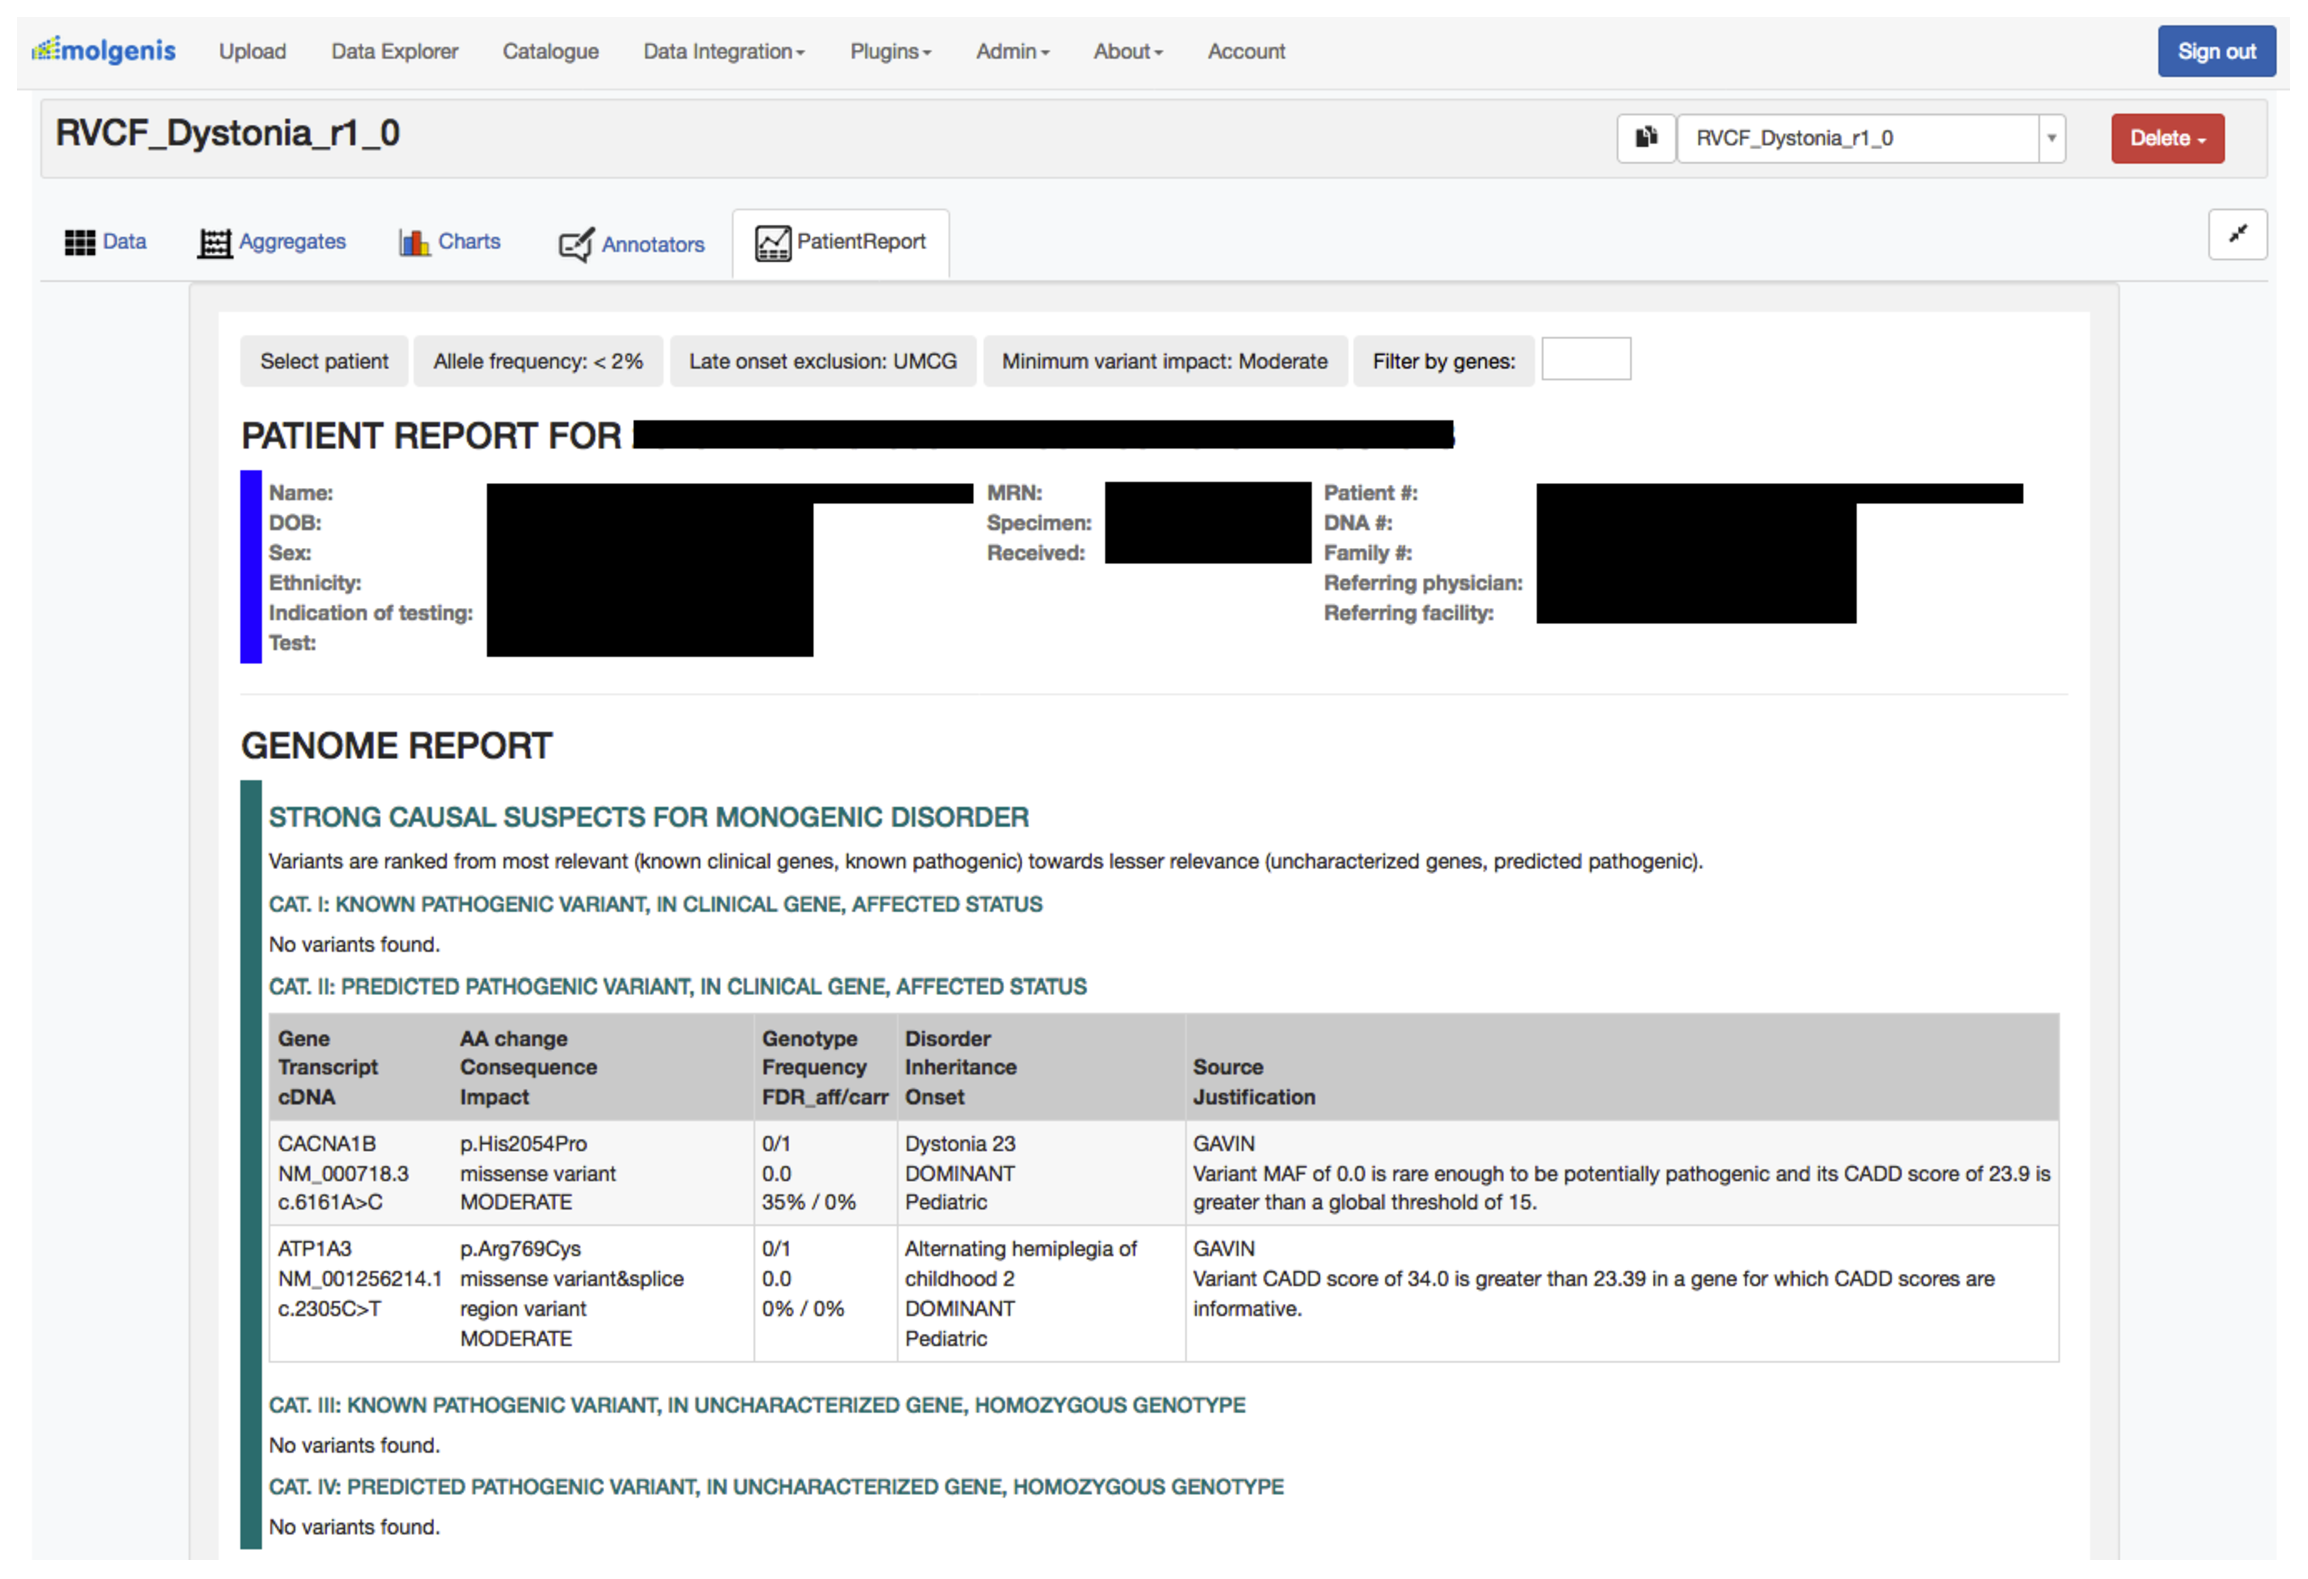
\includegraphics[width=1.0\linewidth]{img/frameworkforgenomics_patientreport}
\caption[Example screenshot of a patient report]{Example screenshot of a patient report generated in MOLGENIS. Sensitive information has been blacked out. Reports are created fully automatically using a template engine on an imported rVCF data set. The buttons at the top offers post-render customization options.}
\label{fig:frameworkforgenomics_patientreport}
\end{sidewaysfigure*}

\subsection{Validation tool: evaluation for diagnostics}

Establishing a molecular diagnosis is only possible when enough data is filtered out to allow human interpretation of the remainder while maintaining reasonably confidence that computational pre-filtering did not remove the causal variant.
To estimate the number of variants that were not detected (false negatives or missed), and the number of variants incorrectly implicated (false positives) in our pipeline implementation for genome diagnostics, we set up an automated validation procedure.
These validations can be quickly run as many times as needed to check performance and expected output of pipelines whenever they undergo any change or update.
This allows efficient testing and uptake of new methods for clinical use, which should increase diagnostic yield.

\subsubsection{Estimation of false omission}

First we investigate how many of the pathogenic variants that we want to find are actually detected.
A missed detection, or false omission, is the most worrisome type of error for molecular geneticists and other experts because a diagnosis cannot be established.\\

\noindent\textbf{Public benchmark data}\\
We performed a false omission rate (FOR) analysis on the GAVIN+ interpretation tool (version 1.0) using known pathogenic variants.
First, we calculated gene-specific FOR on the GAVIN\cite{van_der_Velde_2017} benchmark set, a comprehensive gold-standard consisting of 8,087 unique pathogenic variants from various sources (VariBench, ClinVar, MutationTaster and UMCG clinic), in 1,113 genes.
In total we detected 7,598 of the 8,087 (94\%) pathogenic variants. For 889 (out of 1,113) genes we recovered all their variants, meaning these genes have a FOR of 0\%.\\

\noindent\textbf{In-house patient variant list}\\
As an additional analysis, we exported the most recent controlled in-house list of interpreted variants from our current clinical diagnostic interpretation software.
In this list there were 980 unique variants classified as Pathogenic or Likely pathogenic.
We recall 936 of these 980 variants, or 95.5\%, consistent with the previous result.
See Figure \ref{fig:frameworkforgenomics_for} for an overview of false omission counts per gene.\\

\begin{sidewaysfigure*}
\centering
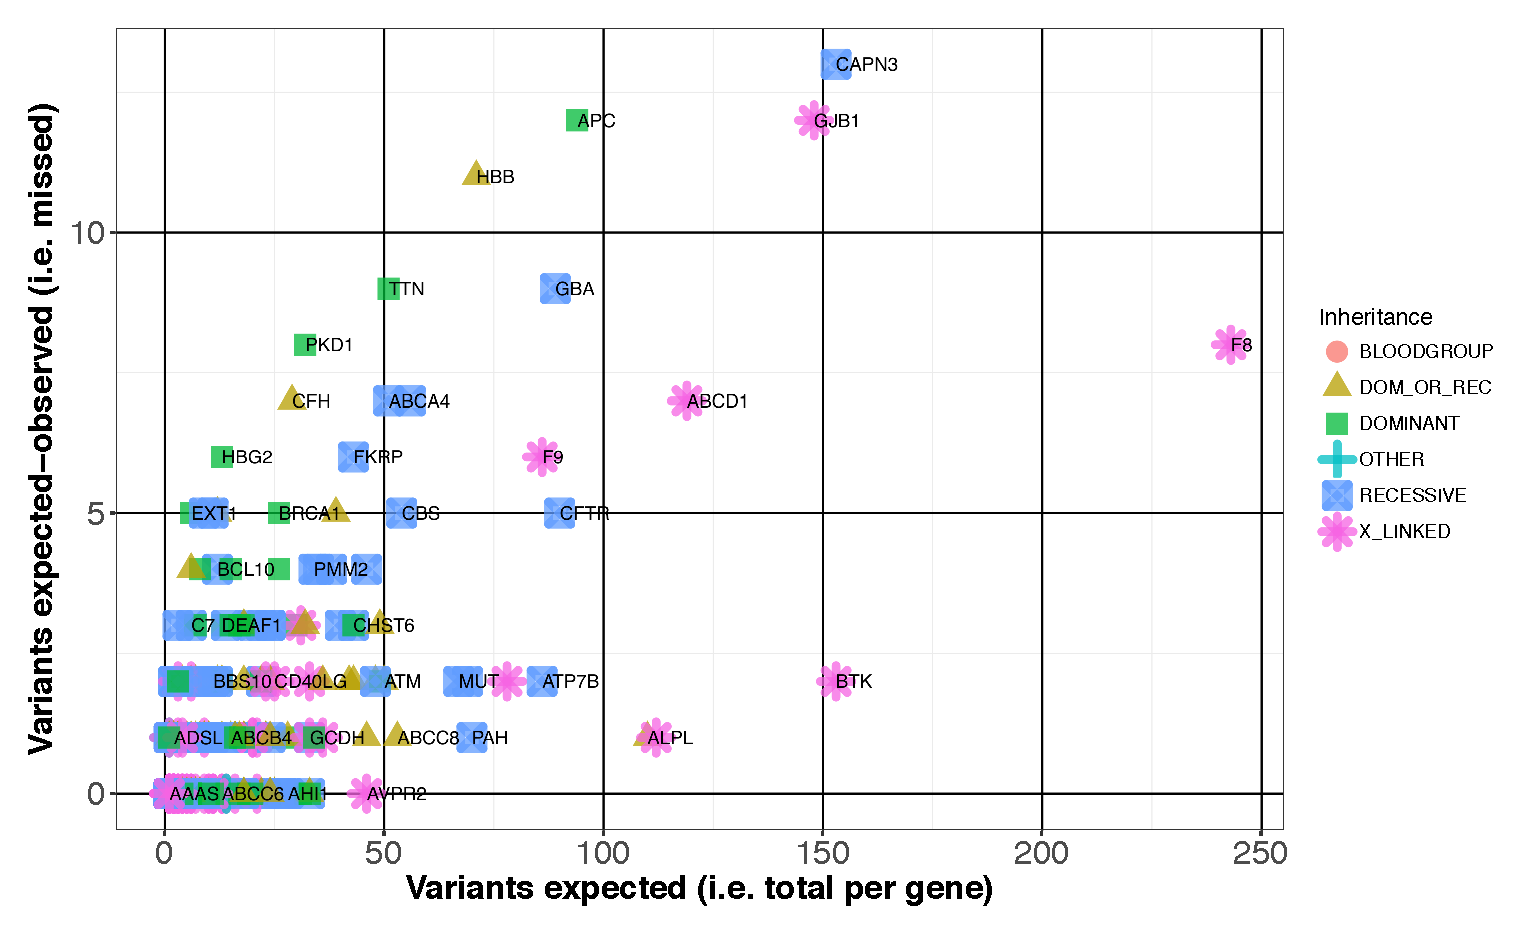
\includegraphics[width=1.0\linewidth]{img/frameworkforgenomics_for}
\caption[GAVIN+ false omission on pathogenic variants]{Counts of GAVIN+ false omission on known pathogenic benchmark variants. Shown are 1,048 (out of 1,113) genes with known inheritance modes from the Clinical Genomics Database.}
\label{fig:frameworkforgenomics_for}
\end{sidewaysfigure*}

\noindent\textbf{In-house patient cases}\\
Lastly, we gathered diagnostic results of 31 patients for whom whole genome or whole exome sequencing was performed to find the molecular cause of their diseases.
These include 21 adults from our clinic (2x pulmonary arterial hypertension, 2x familial cancer, 1x familial hypercholesterolemia, 2x epilepsy, 2x dystonia, 2x epidermolysis bullosa, 10x cardiomyopathy) and 10 critically ill newborns and infants from our rapid genome sequencing program\cite{van_Diemen_2017}.
Executing our diagnostic implementation of the framework resulted in a small number of hits that was checked by molecular geneticists.
In the adult patients, we retrieved the causal pathogenic variant in 18 of 21 cases.
For the 10 newborns, we found the correct mutation in all 10 cases.
In total, we recalled 28 out of 31 variants, or 90\%.
The variants that were missed can be found in Table \ref{table:frameworkforgenomics_missedpatientvariants}.

\begin{sidewaystable}
\begin{tabulary}{\linewidth}{LLLLLL}
  \mbox{Gene~~~~~~~~~} & \mbox{Variant~~~~~~~~~~~} & \mbox{Expert opinion~~~~~~~~~~~~~~~~~~~~~~~~~} & Reason missed & Gene FOR benchmark \\
  \hline
  \rule{0pt}{2.5ex}TTN & c.68225-1G$>$C (splice acceptor-site variant) & Likely pathogenic & Variant CADD score of 24.3 is less than 26.93 in a gene for which CADD scores are informative & 51 / 43 / 15.7\% \\
  \rule{0pt}{2.5ex}NPC1 & c.3011C$>$T (protein change p.Ser1004Leu) & Pathogenic & Variant MAF of 9.39E-4 is greater than 4.36E-4 & 3 / 3 / 0.0\% \\
  \rule{0pt}{2.5ex}LDLR & c.-135C$>$G (5' UTR promoter variant) & Pathogenic & Variant CADD score of 12.88 is less than 16.13 in a gene for which CADD scores are informative & 43 / 41 / 4.7\% \\
  \hline
\end{tabulary}
\caption[Variants that were missed by the GAVIN+]{Variants that were missed by the GAVIN+ interpretation tool. In two instances, CADD scores were in the benign range and in one case the MAF was just too high to be considered pathogenic. The gene FOR benchmark column shows the false omission test results for the corresponding gene as number of variants expected, number recalled and percentage missed (E / R / M\%).}
\label{table:frameworkforgenomics_missedpatientvariants}
\end{sidewaystable}

\subsubsection{Estimation of false discovery}

To gain confidence in our method to predict a variant to be pathogenic for a patient, we estimated how often it would return false hits in genomes of healthy individuals.
A hit here means a potentially pathogenic variant under an acting genotype, e.g. heterozygous for a dominant disorder or homozygous for a recessive disorder.
A very low or even zero number of positive hits in healthy individuals would increase the chance that a hit found in a patient is indeed causal for disease.\\

\noindent\textbf{Public reference genomes}\\
To estimate the gene-specific false discovery rate (FDR) of the interpretation pipeline, we used 2,504 healthy individuals who were whole-genome sequenced in the 1000 Genomes Project\cite{Auton_2015}.
In total, we used 38,097,906 non-intergenic variants observed across chromosomes 1-22, X, Y, and MT.
Per gene, we counted how many unique samples would have one or more variants detected as potentially pathogenic.
This may happen in affected status, meaning that the genotype matches the known inheritance mode of a clinical gene, or if the sample has a homozygous genotype.
For carrier status, the sample is heterozygous, which cannot occur for dominant acting genes.
When applied to the GAVIN+ interpretation tool (version 1.0) described above, we find a mean affected fraction of 0.26\% with a median of 0\%, and a mean carrier fraction is 1.85\% with a median of 0.72\%.
For an overview of gene-specific false discovery rates, see Figure \ref{fig:frameworkforgenomics_fdr}.\\

\begin{sidewaysfigure*}
\centering
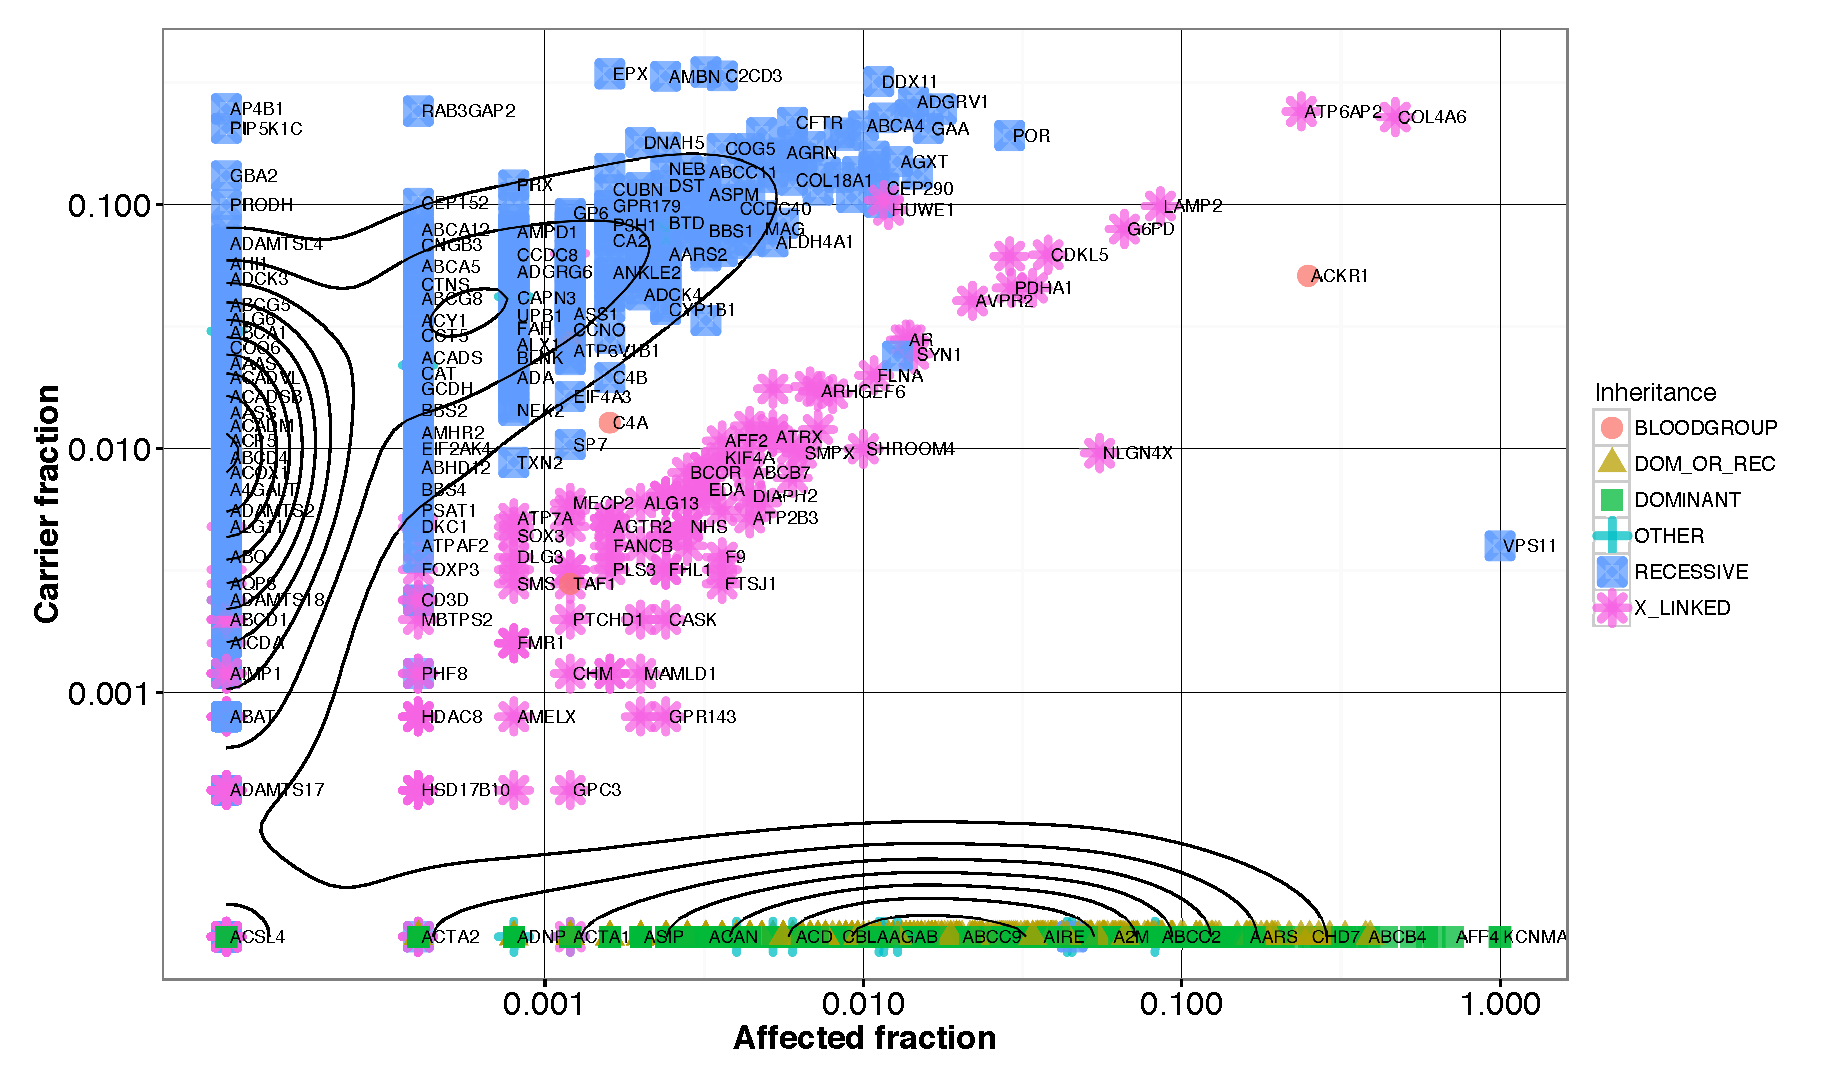
\includegraphics[width=1.0\linewidth]{img/frameworkforgenomics_fdr}
\caption[Estimations of GAVIN+ false discovery rate]{Estimations of GAVIN+ false discovery rate using data from the 1000 Genomes Project. Each point represents the fraction of affected vs. carrier samples, i.e. the number of samples for which a potentially pathogenic genotype was detected under that inheritance mode within a specific gene, divided by the total number of samples. Only genes with known inheritance modes in the Clinical Genomics Database are shown.}
\label{fig:frameworkforgenomics_fdr}
\end{sidewaysfigure*}

\noindent\textbf{In-house patient variant list}\\
We also performed an additional assessment on an in-house list of variants classified by experts (for details, see Methods and Materials).
These variants were rare enough for careful assessment by clinical geneticists as candidates for potential disease-causing effects but were found to be plausibly harmless.
Of the 9,145 variants classified as benign or likely benign, the tool reports 336 hits, resulting in a false positive rate of 3.7\%.


\section{Discussion}

We have reported our development a conceptual framework for structured, automated interpretation of variants with interchangeable components loosely connected by the VCF format.
In addition, we created a first implementation of the framework building on the existing open source MOLGENIS software.
We integrated existing commandline tools as well as a number of new software tools for annotation, analysis and filtering into an executable pipeline for genome diagnostics.
The newly proposed rVCF extension provides an interoperability backbone and, importantly, adds the previously missing link by including information that explains why variants were part of the analysis results.
Furthermore, all rVCF files can be loaded into a web database that generates a report for researchers that provides an overview of clinically relevant findings for medical use.
The content of the reports can be adjusted using option menus, or fully customized by programmers using a template system.
By default, the reports rank variants from most relevant to least relevant.

We have proven our approach with a functional result, but both the framework and its implementation have sparked many ideas for further improvement.
Below we discuss the framework itself, evaluate the implementation results and finally provide direction for future work.

\subsection{Framework considerations}

\subsubsection{Tool interoperability}
The framework defines how tools and data fulfill specific roles within the context of genome interpretation.
However, it does not specify if and how the output of one tool can be connected to the expected inputs of another.
While some output fields are standardized to a degree, such as SnpEff’s 'ANN' field, others are custom or even ambiguous.
For example, an 'AF' field probably refers to allele frequency, but does not make explicit from which population reference this frequency is taken.
An internationally recognized and maintained list of annotation fields might solve this ambiguity, but this agreement needs support from the entire community and requires software changes in most existing tools.
A subtler but easier to achieve strategy would be to use an ontology of genomic annotations to which user can map their software output fields.
To use a familiar reference point, Sequence Ontology\cite{Eilbeck_2005} could be extended with genomic annotations, organized in categories such as 'computational predictions' and 'population allele frequencies'.
In this way, different output annotations could point towards a common reference and software implementations could migrate over time without breaking backwards compatibility.

\subsubsection{Report VCF format}
rVCF specification was defined to capture the relation of any phenotype to any variant including the context in which this association was established.
The information included in rVCF was based on clinically relevant information such as disease phenotype and inheritance, affected individuals, their genotypes, and the reason why this variant was selected.
The data captured in this format can be used to generate genomic reports.
We believe the specification can be easily adopted by other genomic use-cases such as genome-wide association studies (GWAS), quantitative trait loci (QTL) studies, linkage studies or epigenetic studies.
Examples of values for domains other than genome diagnostics, such as model organisms or statistical associations, are shown in Table \ref{table:frameworkforgenomics_rvcffields}.
While the format should be able to accommodate all these applications, additional fields may need to be incorporated to capture important information.
We are curious to find out what these extra requirements are, and we cordially invite the community to adopt, standardize, provide feedback about and improve upon the format.

\subsection{Implementation enhancements}

\subsubsection{Detailed validation output}
The validation tools presented produce false positives and false negatives percentages either overall or per gene.
However, this does not provide insight into the exact differences between the old and a new pipeline or the types of errors made.
To gain more insight, such tools should create a report of their own that compares the errors of the previous pipeline version with the current version.
Information such as 'there is a 14\% increase in false negative splice variants but a 20\% decrease in false positive missense variants' can be very helpful for further improvements or a second tier test to mitigate a particular flaw.

\subsubsection{False discovery analysis}

The GAVIN+ tool was also applied to 2,504 healthy genomes to estimate the rate of false discovery, i.e. to give an indication of how many falsely accused variants can be expected for each gene (see Figure \ref{fig:frameworkforgenomics_fdr}). 
However, since the 1000 Genomes data is based on low-coverage sequencing, it is unclear whether the false positives we found are caused by flaws in our method or by false genotypes present in the data.
Thus, the resulting plot might reflect sequencing bias or genotype calling errors instead of the actual limitations of our method.
To make these estimates more comparable and representative of the data used in a diagnostic sequencing, we need high-coverage whole-genome data from many thousands of  healthy individuals from all ethnic backgrounds.
With the current data, causal variants might be dismissed because of undeservedly high false discovery estimates of the genes they are in.
Another approach that could be used is to use population genomes as a background from which we may calculate diagnostic significance \textsl{P} values for individual patient genomes\cite{Wilfert_2016}.

\subsubsection{Phenotype-matched reports}
The framework implementation we have presented uses only genomic information to generate a patient or research report.
Of course, the clinical features of the sample offer vital clues as to which gene is likely responsible for the disease.
It would therefore make sense to include phenotype-based gene filtering or prioritization to the report.
To make this possible, associations of Human Phenotype Ontology (HPO) terms\cite{Robinson_2010} to their known disease genes could be integrated into the system.
Users can enter HPO terms that match the phenotypes observed in a patient to shorten their list of candidate genes.

\subsection{Increasing diagnostic yield}

\subsubsection{Reducing false positives}
False positives in the context of genome diagnostics are harmless variants that are mistaken for pathogenic.
Predicting many variants as pathogenic translates to a high workload for human experts, who must manually investigate variants before communicating the results to the patient.
To decrease the number of false positives, we can also use specific populations like those provided within ExAC and 1000 Genomes instead of population-wide allele frequency thresholds.
Variants that may be relatively common in one sub-population but not present in others could be filtered out, having low overall MAFs but would logically be considered harmless.
However, with fewer individuals used to ascertain the frequency of a variant within a specific population, the potential bias introduced by randomly including non-representative samples also increases.
This can be addressed by calculating confidence intervals for allele frequencies, and using those in practice instead of the direct allele frequency values.

In addition,  population reference databases such as ExAC offer not only allele counts but also counts of observed homozygous and heterozygous genotypes.
For recessive disease genes, the number of observed homozygous genotypes may be more informative than allele frequency, as the variant may be carried within the population without pathogenic effect.

Lastly, another improvement that could reduce the number of false positives is checking for variants or sequencing artifacts previously classified as benign in ClinVar or other sources such as in-house variant lists.

\subsubsection{Reducing false negatives}
False negatives in the context of genome diagnostics are pathogenic variants that are not detected, a type of error that must be strongly avoided.
The number of false negatives could be reduced by built-in consideration of pathogenic founder mutations.
These can be common enough for a MAF cutoff filter to accidentally remove them before interpretation.
Reporting these variants in international or local databases for use as an interpretation safety net, which is already an optional input for the GAVIN+ interpretation tool, would resolve this issue to a degree.
UMCG genome diagnostics uses an in-house list to identify such variants, but an internationally shared and curated list would be an improvement.

While it is unfortunate that some variants can be missed, estimating miss rates does provide an \textsl{a priori} measure of the difficulty of finding pathogenic variants in their respective genes.
Variants in genes with high estimated miss rates can be double checked when patient symptoms point toward these genes as likely candidates.
This knowledge turns \textsl{unknown unknowns} into \textsl{known unknowns}, empowering the interpretation process and shedding light on potential uncertainties.

\subsubsection{Using structural variation}
This study was focused on processing single-nucleotide variants (SNVs) and small indels, but the structural variation (SV) output of tools such as Manta\cite{Chen_2015} and Delly\cite{Rausch_2012} would also be an important addition to automated interpretation framework.
The regions indicated to be deletions, insertions, duplications, inversions or translocations may be complemented with any SNVs and small indels called by conventional variant callers to increase overall diagnostic yield or to obtain a more complete genomic picture for research projects.

\section{Conclusion}

We have developed and evaluated a framework for structured, stepwise downstream variant analysis.
The aim was a structure that links the different tools and data in this process to enable exchange, reuse and improvement of components of equal scope across institutes.
The novel rVCF intermediate format allows standardized representation of analysis results, and these can be used to quickly create patient or research reports.
We expect that this modular structure will also make it easier to integrate the additional omics technologies that will soon support next-generation sequencing, such as allele specific expression and splicing effects from RNA-sequencing expression, epigenetic markers and metabolomics.

Geneticists have already adopted and learned to rely on best-practice pipelines for NGS variant- and genotype-calling, partly because these tools have matured by the efforts and support of the community but primarily because there is too much raw data to assess by hand.
Given the ever-growing numbers of whole-genome patient sequences we must extend this mentality further downstream towards analysis and interpretation.
To deal with false positives and negatives more effectively, our approach includes automated validation and error estimation tools applied to large benchmark sets to assess the quality and pitfalls of such a pipeline.
We have shown that our diagnostic framework implementation combines and automates the latest knowledge, tools and practices to reduce the time and effort spent on easily resolvable patient cases, a  times savings that will provide human experts with the time they need to solve puzzling cases that will further extend our knowledge of human genetics.


\section{Methods and Materials}

\subsection{MOLGENIS annotation tool}
We developed MOLGENIS CmdlineAnnotator as an extensible annotation framework that works seamlessly in both web and commandline environments.
It has some smart features to maximize the match of input variants (patient) to resource data (context) such as population references.
As an example we can consider the case where the annotation resource has a variant $AGG>A,ATGG$ to denote both the deletion of $GG$ and the insertion of $T$ and our input VCF file has a $A>AT$ variant at the same location.
Though this variant is present in the resource, it would likely be missed because the notation is different.
The CmdlineAnnotator matches this variant by removing but remembering $GG$ from $AGG$ to match the input $A$.
The input alternative allele $AT$ would subsequently be postfixed with $GG$ to form $ATGG$, which matches against the resource successfully.
These slight but relevant differences can be responsible for misinterpretation during analysis.
CmdlineAnnotator version 1.21.1 source code and release are available at \url{https://github.com/molgenis/molgenis/releases/tag/v1.21.1}.

\subsection{Population reference for false discovery analysis}
We downloaded the 1000 Genomes Project phase 3\cite{Auton_2015} release data from \url{ftp://ftp.1000genomes.ebi.ac.uk/vol1/ftp/release/20130502/}.
We annotated genes using SnpEff version 4.2 with these settings: hg19 -noStats -noLog -lof -canon -no-intergenic -ud 0.
Allele frequencies of Genome of the Netherlands\cite{Francioli_2014} release 5 and ExAC\cite{Lek_2016} release 0.3, and CADD scores\cite{Kircher_2014} version 1.3 were annotated using MOLGENIS CmdlineAnnotator v1.21.1.
All VCF FORMAT fields except genotype (GT) were removed from chromosome X and Y to harmonize the data with chromosomes 1-22.
Also, the genotyped samples for chromosomes Y and MT are different from those in chromosomes 1-22.
We wrote a simple tool (SampleFixFor1000GchrYandMT.java) to harmonize the samples for Y and MT, available at \url{https://github.com/molgenis/gavin-plus}.
These fixes now allow all data to be merged by stripping the headers and concatenating the files in the order 1-22, X, Y and MT.
The header from chromosome 1 was added to the merged file with a few INFO lines added that were specific for other chromosomes: LEN, TYPE and OLD\_\-VARIANT from chromosome X, and VT from chromosome MT.
The resulting file was compressed to 8.4G with bgzip and indexed using tabix -p vcf.
It contains 38,097,906 non-intergenic variants and 95,397,156,624 genotypes.
The file is available at \url{http://molgenis.org/downloads/gavin/}.

\subsection{Pathogenic variants for false omission analysis}
We used the GAVIN\cite{van_der_Velde_2017} variant classification benchmark set available at \url{https://github.com/molgenis/gavin}.
This set comprises 25,995 variants from which we select 8,087 pathogenic variants after filtering duplicate genomic positions.
We annotated these variants with SnpEff 4.2, ExAC r0.3, CADD 1.3 and GoNL r5 using MOLGENIS 1.21.1 CmdlineAnnotator.
A heterozygous genotype was added to each variant to enable running of the GAVIN+ automated interpretation tool.
This dataset is available for download at \url{http://molgenis.org/downloads/gavin/}.

We also used a list of variants interpreted by molecular and clinical geneticists at the University Medical Center Groningen according to Dutch medical center guidelines\cite{ACGN}.
More details on the interpretation criteria are provided in Van der Velde \textsl{et al.}\cite{van_der_Velde_2017}.
This list contained 980 likely pathogenic or pathogenic variants and 9,145 benign or likely benign variants after filtering for duplicate genomic positions.
These variants were annotated and processed as above, and access to these data can be requested.

\subsection{GAVIN+ interpretation tool}
We developed the GAVIN+ tool to automate sample genome interpretation.
In a stepwise process, interesting variants are selected (based on hits from GAVIN\cite{van_der_Velde_2017}, ClinVar\cite{Landrum_2015}, or a user-supplied list of variants), followed by a MAF filter, match of genotype to gene inheritance mode, checks for compound heterozygosity and the use of trio or duo sample genotype phasing and de novo variant finding.
GAVIN+ supports multiple alleles per variant that may be present in multiple overlapping gene annotations.
It is implemented in Java 1.8 (\url{https://www.java.com}) as free open source software at \url{https://github.com/molgenis/gavin-plus}.
A comprehensive TestNG (\url{http://testng.org}) test suite ensures correctness and allows further development with a limited chance of introducing bugs.
Dependencies are managed by Apache Maven (\url{https://maven.apache.org/}).
A precompiled, command line runnable version of the tool can be downloaded at \url{http://molgenis.org/downloads/gavin/}.
A demo and manual are available, as are the bundled resources needed to run the tool: ClinVar (any variant matching 'pathogenic' from combined TSV and VCF representations of 11 oct. 2016, 1.5 MB), CGD (version 11 oct. 2016, 380 kB), FDR (version 1.0, 946 kB) and GAVIN calibrations (r0.3, 331 kB).
The implementation insures high performance by using a streaming architecture with as little in-memory buffering as necessary and as much output as possible immediately written to disk.
This results in speeds of millions of genotypes per second.
 GAVIN+ can analyze 300 whole exomes in ~2 minutes or the full 1000G FDR analysis (95,397,156,624 genotypes) in ~2 hours on commodity hardware.

\subsection{Running false omission analysis}
We ran the GAVIN+ tool in a first pass (using -m CREATEFILEFORCADD) to get a list of 34 indel variants that are not yet scored by CADD.
These variants were then scored by a local CADD 1.3 which was installed offline following the instructions at \url{http://cadd.gs.washington.edu/download}.
After scoring, GAVIN+ was run for a second and final pass using arguments: -i GAVIN\_\-FOR\_\-benchmark\_\-goldstandard\_\-nodup\_\-gonl.vcf -g bundle\_\-r1.0/GAVIN\_\-calibrations\_\-r0.3.tsv -c bundle\_\-r1.0/clinvar.patho.fix.11oct2016.vcf.gz -d bundle\_\-r1.0/CGD\_\-11\-oct\-2016\-.txt\-.gz -a fromCadd.tsv -f bundle\_\-r1.0/FDR\_\-allGenes\_\-r1.0.tsv -m ANALYSIS -o RVCF\_\-GAVIN\_\-FOR\_\-benchmark\_\-goldstandard\_\-nodup\_\-gonl\_\-r1.0\-.vcf.
This was followed by a simple tool (FOR.java, available at \url{https://github.com/molgenis/gavin-plus}) to report the false omission rate using original VCF and the rVCF file produced by the GAVIN+ tool.
For each gene, we counted the number of pathogenic variants in the original VCF that we expect to recover.
We divide this number by the observed number of variants in the rVCF as a missed fraction for each gene to estimate how well GAVIN+ detection works for that gene.
All files and results are available at \url{http://molgenis.org/downloads/gavin/}.

\subsection{Running false discovery analysis}
We ran the GAVIN+ tool in a first pass on the 1000G population reference set and got 1,136,050 variants that were not yet scored by CADD.
The local CADD 1.3 tool scored 1,110,509 (97.75\%) of these, meaning that 25,541 of 38,097,906 total variants (0.067\%) remained un-scored.
This allowed GAVIN+ to be run in a second and final pass (using -m ANALYSIS) of the data, resulting in an rVCF file with 381,482 selected variants.
To obtain false discovery rate estimates, we wrote FDR.java, a simple tool that assumes that the hits in the rVCF file are false.
These hits are counted per gene as the number of samples that would have at least one matching genotype under one of two inheritance modes.
A sample is counted as affected when the match is homozygous or compound heterozygous or heterozygous in a known dominant disease causing gene, and counted as carrier when heterozygous in either a recessive disease causing gene or an unknown gene.
A check on phasing may revert compound heterozygotes back to carrier heterozygous multihit status.
The FDR tool outputs a list of 19,230 genes, each with four columns: affected count, carrier count, affected fraction (aff.count/2504) and carrier fraction (carr.count/2504).
Among these 19,230 genes, we find 8,399 with one or more affected samples, 17,878 with one or more carriers, and an overlap of 7,047 genes (17878+(8399-7047)=19230).
This list is further processed to include all 26,023 SnpEff gene names present in the original VCF for which no affected or carrier status was detected.
This was done by first extracting all gene names using GetAllGeneNamesFromVCF.java, followed by using CombineFDRwithAllGenes.java to get the final FDR result file with 26,044 genes.
Note that 21 mitochondrial genes were present in the rVCF file due to ClinVar hits, but these were not annotated by SnpEff in the original VCF file, hence the final result includes slightly more genes.
All result files and intermediates are available at \url{http://molgenis.org/downloads/gavin/}.

\subsection{Visualizing FOR and FDR analysis results}
We wrote a small R script (FDR\_\-plot.R) that uses the FDR result file with 26,044 genes as well as gene annotations from Clinical Genomics Database\cite{Solomon_2013} (file date: August 31, 2016) to plot the observed affected versus carrier fractions.
After merging with CGD we could plot 3,232 of these genes with known inheritance modes.
The color and shape of the points is dependent on the inheritance mode, scales are base 10 logarithmic.
Zero values were replaced with 1e-4 to allow logarithmic scale.
Some genes appear in unexpected plot locations, but can be logically explained.
For instance, CSF2RA appears in the recessive band while being on chromosome X but it is located in the X-PAR1 region.
Conversely, TENM1 appears in the X\_\-LINKED band with a blue icon because it has a mistakenly RECESSIVE annotation.
For only the plotted CGD genes, we find a mean affected fraction of 1.51\% with a median of 0.08\% and a mean carrier fraction of 1.43\% with a median of 0.20\%.
Another R script (FOR\_\-plot.R) visualizes the FOR result file with 1,113 genes.
After merging with CGD we can plot 1,048 of these genes with known inheritance modes.
Again the color and shape of the points is dependent on the inheritance mode.
All scripts and required files are available at \url{https://github.com/molgenis/gavin-plus}.

\subsection{MOLGENIS reporting tool}
To store and visualize the rVCF files produced, we used a modified version of MOLGENIS 1.21.2\cite{Swertz_2010a}.
Users can simply import rVCF files via the standard Data Importer, which can then be viewed in the Data Explorer.
To create the custom reports, we used the Free\-Marker template engine (\url{http://freemarker.org}).
The templates should be placed in the mol\-gen\-is/mol\-gen\-is-app/\-src/\-main/\-resources/\-templates/ folder, and adhere to this naming scheme: view\-[report\-name]\-entities\-report.ftl.
For instance, a Patient\-Report should be named view\-Patient\-Report\-entities\-report.ftl.
The templates are then added as an additional tab for a dataset by clicking the Configure button, and in the Reports box define this link using [report\-name]:[data\-set\-name].
For instance, we connect the Patient\-Report to an rVCF named Cardio using Cardio:\-Patient\-Report.
Multiple links can be separated using commas, e.g. My\-Research\-Exomes:\-Gene\-Report,\-Dystonia:Patient\-Report,\-Cardio:\-Patient\-Report.
The used MOLGENIS and created templates are available at \url{http://github.com/joerivandervelde/molgenis}.

\section*{Acknowledgements}
We thank Kate McIntyre for editing.

\section*{Funding}
We thank BBMRI-NL for sponsoring the above software development via a voucher.
BBMRI-NL is a research infrastructure financed by the Netherlands Organization for Scientific Research (NWO), grant number 184.033.111.
We also thank NWO VIDI grant number 016.156.455.
We acknowledge the support from the Netherlands CardioVascular Research Initiative: "the Dutch Heart Foundation, Dutch Federation of University Medical Centres, the Netherlands Organisation for Health Research and Development and the Royal Netherlands Academy of Sciences" for the GENIUS project "Generating the best evidence-based pharmaceutical targets for atherosclerosis" (CVON2011-19).

\subsection*{Authors' contributions}
KJV, MS designed the conceptual framework.
KJV, BC, DH and FK developed the software and processed the data.
MMV, CCvD, KMA and BSR performed patient DNA variant interpretation and diagnostic validation.
KJV drafted the manuscript with input from LFJ, EC, DH, FvD, FK, KMA, BSR, RJS and MAS.
All authors contributed to the development of the framework and evaluated one or more components.
All authors read and approved the final manuscript.

\section*{Competing interests}
The authors declare that they have no competing interests.

\chapter{Discussion and Perspectives}
\label{chap:discussion}

{ \Large \leftwatermark{
\put(-67,-66.5){ 1 }
\put(-67,-91.5){ 2 }
\put(-67,-116.5){ 3 }
\put(-67,-141.5){ 4 }
\put(-67,-166.5){ 5 }
\put(-67,-191.5){ 6 }
\put(-67,-216.5){ 7 }
\put(-76.5,-250){\includegraphics[scale=0.8]{img/thumbindex.eps}} \put(-67,-241.5){ {\color{white} 8 }}
} \rightwatermark{
\put(350.5,-66.5){ 1 }
\put(350.5,-91.5){ 2 }
\put(350.5,-116.5){ 3 }
\put(350.5,-141.5){ 4 }
\put(350.5,-166.5){ 5 }
\put(350.5,-191.5){ 6 }
\put(350.5,-216.5){ 7 }
\put(346.5,-250){\includegraphics[scale=0.8]{img/thumbindex.eps}} \put(350.5,-241.5){ {\color{white} 8 }}
}}

\newpage

\subsubsection*{Abstract}

The enormous wealth of data generated in the life sciences presents us with incredible opportunities to improve medical genetics, but also with an equally big bioinformatics challenge to fulfill this promise.
The scope and complexity of this challenge is exacerbated by the increasing speed at which new methods, tools and data sets become available across a wide range of disciplines ranging from statistics to computer science and from model organisms to clinical validation.
In this thesis, I contributed a number of bioinformatics models, methods, and integrated systems thereof as infrastructure to enable rapid translation of these new resources into medical applications.

\subsubsection*{Introduction}

In this thesis I first developed new data management and processing models in chapter \ref{chap:xgap} and implemented these to store, integrate and visualize model organism data in chapter \ref{chap:xqtl}.
By connecting human disease phenotypes to model organisms, I showed that this approach can be used to discover new disease leads in chapter \ref{chap:wormqtl}.

I then investigated how existing methods for computational estimation of variant deleteriousness can be used to predict pathogenicity classification with high precision and recall in chapter \ref{chap:caddmmr}.
In chapter \ref{chap:gavin} I generalized this method to thousands of genes, and molecular geneticists can now use an integrated online system to classify patient DNA variants in the context of large reference data.

While new methods and data become available at ever increasing speeds, their implementation in clinical practice lags behind because of the time needed to validate and implement them into clinical practice.
To implement and validate new analysis protocols rapidly and efficiently in research and clinical practice, we need a streamlined automated pipeline for data processing, decision making, and reporting of results.
I therefore developed a software system for structured variant interpretation, currently adopted in routine diagnostics, that combines new methods and models with existing tools and knowledge databases in chapter \ref{chap:frameworkforgenomics}.

In this chapter I will consider the meaning and implications of the work presented in this thesis and look to the future potential and oncoming challenges of the field.
I first discuss in section \ref{modelsection} the successes and challenges of flexible models to capture, integrate (\ref{modelsection_integration}), share and reuse life science data (\ref{modelsection_reusable}).
I address how more people could benefit from these innovations (\ref{modelsection_spreadsheet}), and if perhaps smarter technologies are needed to get more value from complex data (\ref{modelsection_future}).

Second, I consider the challenges of method development, in which data plays a critical role in section \ref{methodsection}.
The importance of data quantity and quality is exemplified (\ref{methodsection_data}), as well as pitfalls in method benchmarking (\ref{methodsection_benchmarking}).
I highlight future ways to overcome difficulties in finding (\ref{methodsection_finding}) and running appropriate methods (\ref{methodsection_running}).

Finally, I examine how to better implement complex systems for application to medical genetics in section \ref{systemsection}.
Crucial aspects such as sharing of workflows (\ref{systemsection_reusable}) and community expertise (\ref{systemsection_community}) are discussed, and I suggest future work on multi-omics analysis (\ref{systemsection_multi}) and semantic protocols (\ref{systemsection_semantic}).
For each of the sections I will summarize key question and key points.


\sectionmark{Flexible models for life science omics data} % extra to get the top mark okay..
\section{Flexible models for life science omics data} \label{modelsection}
\sectionmark{Flexible models for life science omics data}

Life science data can be stored, managed and queried in a multitude of different ways, each with their own advantages and drawbacks.
In this section, I discuss various models and aspects involved in confronting the life science data challenge.

\subsubsection*{Key question and points of this section}

\textsl{How should data models be designed to integrate, reuse and share data from life science experiments in order to extract knowledge that benefits medical genetics?}

\begin{tcolorbox}[width=\textwidth,colframe=deeporange,colback={white},title={Key points},colbacktitle=deeporange,coltitle=black,enhanced]
  \begin{itemize}
    \item We have researched and evaluated different data integration models that make genotype-phenotype analyses more contextual and insightful (\ref{modelsection_integration}).
    \item Some applications demand greater data model flexibility, but the loss of predefined data classes presents new issues (\ref{modelsection_reusable}).
    \item Ontologies can be used to give explicit meaning back to the data, allowing methods and tools to again perform cross-set analyses (\ref{modelsection_reusable}).
    \item Managing growing quantities of life science data in spreadsheets and flat files is problematic, therefore more should be done to increase uptake of better alternatives (\ref{modelsection_spreadsheet}).
    \item Data is being shared, but without smart storage algorithms it remains difficult and time consuming to ask even basic questions (\ref{modelsection_future}).
  \end{itemize}
\end{tcolorbox}

\subsection{Integration of heterogeneous omics data} \label{modelsection_integration}

Methodological (re)use of all available life science data is difficult.
Making data suitable for reuse requires structured storage with sufficient metadata to allow retrieval and interpretation, which is troublesome and time consuming to achieve.
In addition, various storage paradigms are needed to complement traditional databases because data volumes are large and database structures often complex and highly heterogeneous\cite{Swertz_2007}, which limits interoperability and integrateability of these data.
Data covers a wide variety of phenotypic measurements including age, gender and height; answers given in questionnaires; detailed clinical observations; and large-scale molecular measurements such as DNA sequencing, gene expression, metabolomics and proteomics.
Moreover, these data may be collected from many subjects, at different timepoints, from multiple tissues, using a various wet and dry laboratory protocols.
Finally, rapid development of new profiling techniques and analysis methods requires data infrastructure to rapidly change to accommodate.

\subsubsection*{The eXtensible Genotype and Phenotype model}

We investigated how data models and supporting software systems should be (re)designed to accommodate this heterogeneity and to be effective in handling these data.
The first result was the XGAP data model developed to capture a variety of life science data that is described in chapter \ref{chap:xgap} and summarized in Box 1.

\begin{tcolorbox}[width=\textwidth,colframe=deeporange,colback={white},title={Box 1: Brief explanation of the XGAP data model},colbacktitle=white,coltitle=black,enhanced]
The innovative XGAP model facilitates integration of a wide range of data sources into one conceptual framework by enabling researchers to define observations as any combination of subjects (the thing being observed) and trait (the measurable quality).
As a result, data can be flexibly stored, eliminating the need to define the exact storage requirements for experimental data, which is impossible beforehand and moot after project completion.
For example, definitions of concepts such as 'Gene', 'Marker', 'Individual' or 'Metabolite' remain constant, but they can be used to create any dataset while the application is running.
Then gene expression data can be defined as 'Gene' $\times$ 'Individual' with a numeric value at each combination and a genotype map as 'Marker' $\times$ 'Individual' with categorical values, e.g. 'AA', 'CC', 'AC'.
After QTL analysis, the result then can be defined as 'Gene' $\times$ 'Marker' where each value indicates the statistical strength of the association between gene expression and genotype.
\end{tcolorbox}

XGAP’s flexibility is a sharp contrast to traditional applications built on relational databases that need to be taken offline for redesign when a new data modality comes in.
A life science database can now be created when a research project starts and experimental measurements plus contextual data from external providers, e.g. gene annotations or pathway definitions, added naturally as the project progresses.

We implemented XGAP into the MOLGENIS\cite{Swertz_2010a} software toolkit that generates database software infrastructure from data model and user interface specifications.
By combining the MOLGENIS software and XGAP datamodel as a foundation, we now can implement generic life science databases that can handle almost any omics/QTL data.
We published this system as xQTL workbench in chapter \ref{chap:xqtl}.
This system can handle any genotype-to-phenotype experiments and can be used as a template to create data portals for specific research areas.
We demonstrated the added value of xQTL first in \textsl{C. elegans} research\cite{Snoek_2012}, then added a translation from model organism to human disease genetics.
The resulting WormQTL\textsuperscript{HD} database\cite{van_der_Velde_2013a} is described in chapter \ref{chap:wormqtl}.
Its built-in visualization tools can be used to find clues for the molecular workings of human disease in almost 100 online-accessible datasets.

\subsubsection*{When even more flexibility is needed}

The XGAP model’s power comes from its fifty-fifty balance between static data structure (the underlying structure does not change when new data is loaded) and dynamic modeling (the structure can be easily extended and adapted and depends on the genes and phenotypes in the experimental data).
The static structure acts as a stable template that enables development of new software tools that then will work on all data loaded because the tools know what data structure to expect.
At the same time new data modalities can be rapidly accommodated using the flexible structure.

However, there are drawbacks to using (partially) static data structures.
It requires users to familiarize themselves with a data model, and limits the attributes that can be used to express information while simultaneously burdening the user with often unnecessary attributes.
An attribute is a property of the object type being described.
An object of the type 'car', for instance, can have the attributes 'brand', 'model', 'color', and 'year of construction'.
Pre-defining the attributes for data in life sciences can be very convenient for some uses, for instance if they want to automatically connecting genomic data to a genome browser.

Nevertheless, we found that more flexibility is better in some other cases.
Therefore, when we developed MOLGENIS 2.0, we created the even more flexible EMX (entity model extensible) storage model.
In MOLGENIS 2.0, the user uploading the data has full control over all aspects of the data model, meaning that tabular data can be defined at column and data type level, as well as cross-linked in any way.
This allows use of XGAP or other data models if desired.

Together with collaborators, we evaluated the models in many other online databases for various domains within life sciences\cite{Adamusiak_2012}.
Figure \ref{fig:discussion_molgenisfamily} shows the two main paths in evolution (XGAP and EMX data modeling) and a selection of currently active software applications.
These applications are powered by the MOLGENIS platform which allows flexible generation and configuration of database application.

\begin{figure*}
\centering
\includegraphics[scale=0.7]{img/discussion_molgenisfamily}
\caption[The MOLGENIS family of software]{The MOLGENIS family of software, data models and applications. The core software and models (top left corner) form the basis for a variety of applications, with those in green boxes directly built from the XGAP data model. The types of applications are indicated with an $\boldsymbol{\alpha}$ for research portals, $\boldsymbol{\beta}$ for patient registries, $\boldsymbol{\gamma}$ for diagnostics support, and $\boldsymbol{\delta}$ for biobank catalogues. Blue text indicates a peer-reviewed published article.}
\label{fig:discussion_molgenisfamily}
\end{figure*}

\subsection{Making omics data reusable across systems} \label{modelsection_reusable}

The most recent versions of MOLGENIS allow the user to define and import any data structure.
This is highly appreciated by users as it provides complete freedom to upload whatever data they like.
MOLGENIS uses a simple tabular format that contains both the data itself and its meta-data describing the flexible attributes with strongly-typed values.
After import, data set columns can be added, deleted or redefined if needed.
Data values can cross-reference to other datasets or rows within datasets to create a complex ad hoc data model.
Users can thus create a database perfectly tailored to their storage needs that can be re-tailored whenever those needs change.
The learning threshold of creating and managing such a database is low, and it encourages people to upload and connect any data they find relevant.
However, because the semantics of the data are now no longer explicit, this presents a new challenge.

\subsubsection*{Need standard model building blocks}

While it is now much easier to bring data together into one MOLGENIS system, the cost of this freedom is the loss the explicit meaning of the data, as compared to XGAP.
This greatly limits data re-use because data cannot be easily integrated with other datasets and analysis tools cannot be used.
In other words, for data to be reusable its semantics must be clear so humans as well as software can understand and know what to do with it. 
Users A and B may both upload a set named 'Genes', but the system does understand whether these actually refer to the same concept.
The same problem applies to any attributes within these data sets.
Perhaps they both have a 'Position' column, but one may be measured in centimorgan and the other in base pairs.
Even if the units are the same there may be crucial contextual differences, for example base pair positions that are derived from different genome builds.
This uncertainty makes it impossible to reuse tools and methods because certain necessary attributes cannot be automatically connected.

To deal with this issue, the latest MOLGENIS versions use small data models to enable implementation of standard analysis protocols without limiting the flexibility of the system.
Some data has a very predictable and often reoccurring structure. A good example is the 'genomic location’ tied to variants and other features of the DNA.
The attributes of these genomic locations are usually chromosome, position, genome build, reference and alternative base, which are automatically mapped to a micro-model and understood by the system so that tools such as the genome browser can immediately visualize the data.

\subsubsection*{Use of ontologies}

The micro-model solution is an efficient way to deal with highly predictable data.
However, most flexible data will still not be understood by the system and therefore not easily connected, integrated and analyzed.
Note that the difference between a data model and an ontology is subtle but significant, and therefore we clarify this in Box 2.

\begin{tcolorbox}[width=\textwidth,colframe=deeporange,colback={white},title={Box 2: Difference between data model and ontology},colbacktitle=white,coltitle=black,enhanced]
Ontologies can be thought of as dictionaries that define terms, with the special addition that terms can be related to each other.
Data models can be thought of as floor plans that offer explicit structure, while the definitions of the concepts used are implicit.
For example, a floor plan could specify how a living room is connected to the other rooms and show the arrangement of the furniture, whereas an ontology would define the concepts of a living room and elaborate on known types of furniture.
People who used different building plans to construct their house can use the ontology to refer to their now shared understanding of a living room, and find out if they both have a couch in it.
\end{tcolorbox}

To overcome this problem, we enable users to annotate or 'tag' their free-form data with additional meta-information that explains what the data means.
The database must contain concepts such as 'Position' measured as 'Integers' on reference build 'GRCh37' for 'Homo sapiens'.
These concepts can then be mapped on the sets, rows and columns of data sets imported.
Tools use these tags to understand the meaning of the data, which ensures that queries and tools can be reused between heterogeneous datasets.

The meta-data used to annotate data with meaning are called \textsl{ontologies}, which are common dictionaries of agreed-upon, well-defined terms and their relationships.
Building an ontology through input from an international community of domain experts ensures a shared point of reference for the clear communication of meaning.
Annotating data with ontologies offers many advantages in terms of connectivity and reasoning, but requires a significant investment of expert’s time.
To drastically lower this burden, we have developed strategies for automated matching of terms to ontologies\cite{Pang_2014} and for smart matching values to coding systems\cite{Pang_2015}.
The resulting systems allow users to harmonize data items and values in a fraction of the time it would normally cost, thereby enabling pooled data analysis for higher statistical significance.
The MOLGENIS online data platform can assist users to quickly interconnect their data via semantic annotation\cite{Pang_2015}.

\subsubsection*{Ontologies for medical genetics}

Structured ontologies also provide computational advantages.
Ontologies may be expressed as graphs of connected terms, typically a tree-shaped hierarchies where a broad root term branches out into more specific terms.
Famous ontologies used in medical genetics include ICD\footnote{http://www.who.int/classifications/icd/en} and SNOMED-CT\footnote{http://www.snomed.org} for diseases, and Gene Ontology\cite{Ashburner_2000} to describe genes.

The Human Phenotype Ontology\cite{Robinson_2010} (HPO), shown in Figure \ref{fig:discussion_hpograph}, is an ontology of particular usefulness.
HPO terms are becoming an integral component of clinical work in many medical centers, including the UMCG\cite{van_Diemen_2017}, where they are used to convey patient symptoms to the decision support software.
Symptoms can be expressed in HPO terms that may be broad or specific.
Likewise, diseases may be expressed as collections of multiple HPO terms.
Computer algorithms can accept HPO terms as inputs and take advantage of the underlying graph structure, for example, to find a known disease that best matches a set of input symptoms.
The paths between the terms are used as a distance measure, and advanced methods can even calculate semantic distance between collections of terms weighted by information content\cite{Resnik:1995:UIC:1625855.1625914}.
This clears the way for advanced tools\cite{Girdea_2013} that can guide or support a genomic diagnosis with a robust phenotypic match of patient symptoms to a known disorder for which the causal gene is known.

\begin{figure*}
\centering
\includegraphics[scale=1.0]{img/discussion_hpograph}
\caption[Graph of the Human Phenotype Ontology]{Graph of the Human Phenotype Ontology colored by eccentricity, i.e. the distance to root node, from 0 (green) to 13 (red). The blue box shows a zoomed-in view so that labels can be read and the hierarchical structure becomes apparent. This graph has 11,044 vertices and was visualized using CytoScape (\url{http://www.cytoscape.org}) on the OBO file of HPO downloaded June 2015.}
\label{fig:discussion_hpograph}
\end{figure*}

\subsection{Spreadsheets in the era of big complex data} \label{modelsection_spreadsheet}

Many researchers, clinicians and other specialists use unsophisticated data storage methods such as spreadsheet documents.
While spreadsheets are a useful means for interacting with tabular data, they are not intended to be used as local databases for serious long-term data management.
As datasets in spreadsheets grow in size and complexity, many problems arise regarding data consistency\cite{Ziemann_2016}, corruption (e.g. the 'autocorrection' of gene names that look like dates\cite{Zeeberg_2004}), availability, versioning, performance, backups, multi-tenancy and security - nor do local spreadsheets support FAIR principles\cite{Wilkinson_2016,Wilkinson_2017} that encourage data to be Findable, Accessible, Interoperable and Reusable.

\subsubsection*{Making relational database technology accessible}

Relational database technology has developed over the many decades since its invention\cite{Codd_1970} to specialize in highly structured and consistent management of high-dimensional tabular data.
Frameworks such as MOLGENIS enable the creation of front-end web interfaces that allow relational databases to be operated in a more visual and user-friendly way.
Many software applications that were developed with the MOLGENIS framework, shown in Figure \ref{fig:discussion_molgenisfamily}, prove that this approach brings the advantages of relational databases to a variety of life science data applications that might otherwise remain hidden and vulnerable in local spreadsheets.

\subsubsection*{The challenge of big data}

Relational databases are not always an appropriate storage solution.
Huge files are currently being produced by automated data processing tools by high-throughput technologies such as whole-genome DNA sequencing.
With costs dropping and thousands of samples sequenced daily, the data is rapidly growing from terabytes to petabytes and beyond.
It would therefore be highly impractical to store each atomic value from these data in a relational structure because there is no need for this data to be query-able and a significant amount of additional disk space would be needed to index the data.

However, when thousands of individuals are profiled over many years and their data analyzed by many researchers in different projects, it is inevitable that data is lost track of.
Retrieving specific samples in that situation would involve a costly exercise in 'forensic bioinformatics'.
Projects that want make use of the data, for example a combined re-analysis of undiagnosed patients with a cardiomyopathy indication, would have to spend a significant amount of time to simply retrieve the right samples.

\subsubsection*{How to find and access large files}

A catalogue system powered by a relational database can be used to store sample metadata and file locations, along with detailed provenance of how the sample was processed and analyzed, and of the results.
Using information such as patient phenotype, tissue sampled, sequencing platform and processing software used, data of interest can be quickly found and used for analysis.

A publicly available example of such a big data catalogue is the European Genome-phenome Archive \cite{Lappalainen_2015}, which currently contains everything from raw sequencing files to genotypes called to phenotypes.
The data is organized in studies and data sets, and enriched with the provenance of samples and the technology used for analysis, e.g. "Affymetrix 500K" or "Illumina HiSeq 2000".
This allows researchers to find data appropriate for their (meta-)analysis amongst the petabytes of deposited files based on biological-, laboratory- and digital provenance.

\subsubsection*{Hybrid solutions for large data queries}

Combining relational and file-based storage can also be an effective solution.
The applications developed based on the XGAP data model, such as WormQTL\textsuperscript{HD}, employ a hybrid file-relation storage strategy.
The rows and columns link to entries in a relational database, such as Markers and Genes, which can be queried as usual, while the large data in matrix form are stored as a two-dimensionally indexed binary file.
Using the query results, data selections from the matrix based on rows and columns can be made very quickly.

The result of this hybrid design is great performance with minimal overhead and disk space requirements, but its drawback is that sorting and filtering operations on non-indexed matrix values are slow.
These queries are however not important for the main use-cases of this database, so the overall solution worked out very well.
This shows that no solution is perfect, but the success of a system does depend on the storage strategy chosen.

\subsubsection*{Basic data management training for all life science researchers}

We have shown many different models, methods and tools to manage life science data, from relational databases with static and dynamic models to relational-file hybrids and file-catalogue systems.
There is no single “best” solution: each of these approaches represents a valid solution for different storage and query requirements, which just underscores the need for flexible systems that can adapt to future data structure needs and switch to storage backends that scale to bigger data volumes when required.

However, the average researcher has little interest in the technical background of these solutions and simply wants a system that capable of serious data management that is still as comfortable to use as a spreadsheet program.
Making the transition requires an investment of time and energy that is sometimes not well understood and/or seen as too burdensome.
Parties that offer data management solutions may have a responsibility to underscore the importance of helping people to use better data management.
We suggest number of actions to facilitate the uptake of better data management tools in Box 3.

\begin{tcolorbox}[width=\textwidth,colframe=deeporange,colback={white},title={Box 3: Actions towards uptake of better data management tools},colbacktitle=white,coltitle=black,enhanced]
\begin{enumerate}
  \item Raising awareness of the dangers and limitations of using spreadsheets and other inappropriate solutions for data management. This is also the mission of the European Spreadsheet Risks Interest Group\footnote{\url{www.eusprig.org}}.
  \item Increasing the visibility of alternatives by shifting the focus of publications, workshops and presentations from specific applications back towards the importance of underlying technologies such as the MOLGENIS platform.
  \item Making demonstrations publicly usable in an unrestricted but private way to those who are interested. Subsequently, non-technical users should be able to immediately create secure instances in the cloud suitable for sensitive data. For technical users, it should be simply to run the software on their own servers.
  \item To keep initial interest alive, the thresholds of starting to use these applications must be as low as possible. Data management should be user-friendly overall, but it is critical that systems be fault-tolerant so aspiring users are not punished by having to fix many small mistakes when importing their data. Data should also be importable in the simplest of formats and even via direct entry, i.e. similar to using spreadsheet software.
  \item Those exploring the system more deeply must experience clear benefits and advantages. For instance, a user-friendly data explorer should offer powerful options to find, filter, sort and plot the data, as well as guarantee consistency, security and easy sharing with colleagues.
\end{enumerate}
\end{tcolorbox}

\subsection{Future perspectives of sharing life science data} \label{modelsection_future}

The life science and molecular medicine community is gathering, using and sharing tremendous amounts of data. 
Popular published data resources include the Genome of the Netherlands\cite{Francioli_2014}, Ar\-ray\-Ex\-press\cite{Rustici_2012}, 1000 Ge\-no\-mes Pro\-ject\cite{Auton_2015}, Va\-ri\-Bench\cite{Nair_2012}, Blood eQTL brow\-ser\cite{Westra_2013}, database of Geno\-types and Pheno\-types\cite{Mailman_2007}, Clin\-Var\cite{Landrum_2013}, Exome Aggregation Consortium\cite{Lek_2016}, genome Aggregation Database\footnote{\url{http://gnomad.broadinstitute.org/}}, RNA-seq ASE brow\-ser\cite{Deelen_2015}, Eu\-ro\-pe\-an Nu\-cleo\-tide Ar\-chive\cite{Leinonen_2010} and Ge\-no\-type-Tis\-sue Ex\-pres\-sion\cite{Lonsdale_2013}.
Making these data open and freely available generates a higher number of citations and increases their overall prestige, which should clearly outweigh any benefits of 'keeping data to yourself'.
Further, an increasing number of (often high-impact) scientific journals and public funding bodies require any data in publications to be openly accessible (the ideal) or at least available on request.
In fact, it is now possible to publish data as standalone resources, for example in journals such as \textsl{Scientific Data} or initiatives such as \textsl{DataCite}.
The field of genetics is indeed a frontrunner "whose sharing of data markedly accelerated progress"\cite{Rosenbaum_2017} compared to fields such as clinical trials.

Indeed, we ourselves opened up dozens of research datasets and results in the WormQTL\textsuperscript{HD} database, free to download without restrictions for anyone interested .
Conversely, the methods presented in chapter \ref{chap:caddmmr}, the CADD scores for MMR genes, and GAVIN in chapter \ref{chap:gavin}, could not have been developed without free and publicly available datasets.

\subsubsection*{New query options are needed for humans and computers}

While incredible datasets are currently being generated, the development of software tools to interact with these data seems to be lagging behind.
Even relatively simple questions such as "How many variants at exon 10 of the TTN gene are exclusive for individuals of Asian descent?" cannot easily be asked because
(i) most resources do not have an adequate query interface,
(ii) query interfaces do not understand or support the question, and
(iii) there is no cross-database "Google-like" interface to query all potential sources at once.
We could fulfill the promise of systems biology research to create understanding of life in a bigger context by being able to routinely run deep complex queries across our complete knowledge of organisms, phenotypes, populations, tissues, metabolites, genetics, drugs, and so on.

\subsubsection*{Ontologies, semantics and FAIR solutions}

This situation can be improved by increased usage of ontologies.
Data may be expressed as \textsl{nanopublications}, i.e. predicated relationships between two ontological concepts with provenance attached.
For example, we can express knowledge into formal terms as follows:
the CENPJ gene (\url{http://bio2rdf.org/geneid:55835}) has a statistical association (\url{http://semanticscience.org/resource/SIO_000765.rdf}) to Seckel Syndrome (\url{http://bio2rdf.org/omim:210600}) of 0.00006562\footnote{Example taken from: \url{http://nanopub.org/wordpress/?page_id=57}.}.
Data can be freely reasoned upon once expressed in a formal and semantic way, as demonstrated in case studies\cite{Mina2015}.
The underlying RDF\cite{RDF-PRIMER} (Resource Description Framework, a way to semantically describe data) and SPARQL\cite{Prudhommeaux08} (Simple Protocol And RDF Query Language, a way to question semantic data) technologies are supported by the Linked Data initiative\footnote{\url{http://linkeddata.org}}, which aims to connect structured data on the internet, essentially turning it into a giant database.
It has also been shown that semantic queries can indeed be used for both generating and evaluating hypotheses\cite{Mina2015,Callahan_2011}, and assist in genomic variant prioritization\cite{Boudellioua_2017}.

Although some large organizations offer proper RDF access\cite{Jupp_2014} and third-party tools are written for others\cite{Anguita_2013}, this technology is hardly a cornerstone of modern life science databases.
It can be quite labor-intensive to completely ontologize a database for RDF support and setting up an active SPARQL endpoint.
The FAIR principles\cite{Wilkinson_2016,Wilkinson_2017} offer an alternative with much lower barriers.
FAIR is essentially a checklist to guide technical solutions and their practical applications to make data more Findable, Accessible, Interoperable and Reusable.
When fully realized, every aspect of data would be annotated with semantic metadata for complete and seamless reusability.
The MOLGENIS/XGAP work presented in this thesis are in that sense FAIR systems, created before that term was coined.

Given the challenges of building and using datamodel based storage systems this is not always attainable.
However, the guidelines can be followed to make data discoverable and searchable in simpler ways, which is always better than not at all.
An example of an easy and lightweight solution to make resources better findable by search engines is to add Bioschemas\footnote{http://bioschemas.org} semantic markup.
Other databases, platforms and initiatives such as Dataverse\cite{Crosas_2016}, FAIRDOM\cite{Wolstencroft_2016}, ISA\cite{Sansone_2012} and Open PHACTS\cite{Harland_2012} showcase other implementations and applications that are based on FAIR principles.

\subsubsection*{Federated queries require an attitude shift}

In addition to new data models and tools, I think we also need to change our attitude towards sharing and integration of query results.
Data sizes are rapidly increasing and much data is privacy sensitive, factors that make it unlikely that all data relevant to a given study will always be available in one place.
New data analysis paradigms are being developed to address this, of which so-called 'federated analysis', is a prominent example\cite{Gaye_2014,Jochems_2016}.
A federated query is executed on multiple independent locations, after which the partial results are combined into the final answer.
The nature of federated queries on multiple external sources is that the answer of today may be different from the answer of tomorrow.
This can be seen as a limitation, but can also be considered an opportunity where researchers and even clinicians always have access to the latest and greatest knowledge.
Instead of statically versioning complete data sources as a reference point, we must consider making our data dynamic and compensate for perceived uncertainties by storing the questions together with detailed data and source provenance used to compile the answer.

\subsubsection*{Legal aspects of data sharing}

Until here I have discussed life science data sharing from a mostly technical point of view.
It is however important to realize that even the most brilliant solution is pointless if the law precludes sharing and reuse of data.

Currently, data and privacy laws are being revised in light of social media and the other 'tech giants' who are gathering massive amounts of sensitive user data.
While citizens will benefit from better privacy protection, the same rules impede cohort-based biomedical research by requiring participant re-consent every time the data is used\cite{natedit_2015}.

While scientific representatives are gaining concessions on behalf of research, their legal struggle is not yet over.
Establishing fitting international legislation with many stakeholders across cultural barriers is difficult, as is the practical implementation of new rules by the science community\cite{Litton_2017}.

Perhaps by overcoming these legal growing pains, current hindrances for sharing and reusing biomedical data across the international community can be lifted, benefitting researchers and ultimately patients.


\sectionmark{Developing comput. methods for med. genetics} % extra to get the top mark okay..
\section{Developing computational methods for medical genetics} \label{methodsection}
\sectionmark{Developing comput. methods for med. genetics}

So far I have investigated models to store, access, share and query data measured and calculated in life science experiments to gain new insights.
In this section, I discuss challenges and solutions in the development and, more importantly, validation of new methods and algorithms to make most use of all these new data.

\subsubsection*{Key question and points of this section}

\textsl{How can we develop, characterize, find, share and reuse high-quality computational methods as part of new analysis protocols for medical genetics?}

\begin{tcolorbox}[width=\textwidth,colframe=deeporange,colback={white},title={Key points},colbacktitle=deeporange,coltitle=black,enhanced]
  \begin{itemize}
    \item The performance of newly developed methods depends on both the quality and quantity of available data. We must therefore cherish and share gold standard data (\ref{methodsection_data}).
    \item Reporting the strengths and weaknesses of a method in greater detail next to the overall performance is crucial for choosing the right analysis method to obtain better research or diagnostic results (\ref{methodsection_benchmarking}).
    \item We need detailed catalogs where researchers and clinicians can seamlessly find these assessments (\ref{methodsection_finding}) and run the right tool for their data and hypothesis (\ref{methodsection_running}).
  \end{itemize}
\end{tcolorbox}

\subsection{Method dependance on high quality data} \label{methodsection_data}

The genome of an average person contains around 5,000 unique mu\-ta\-tions\cite{Walter_2015}.
To establish a molecular diagnosis in an individual with a suspected genetic problem, we need to quickly reduce the number of candidate variants from thousands to just a few.
Computer algorithms can predict how harmful mutations are, but the strength of these predictions depends on the availability and quality of reference data.
These gold standard reference data are used to develop new algorithms, which are then validated on a similar but independent data set.

In this section we show that both quality and quantity of data have an effect on the predictive power of new methods.
Sharing data is therefore crucial for developing the best possible tools, resulting in more accurate prioritization and less time spent on manual assessment.
We therefore must engage in active international collaboration to set up systems for joint interpretation and open sharing of variants.
To accomplish this goal we need to overcome technical and legal barriers, but it is also a social challenge, as labs can be distrustful of other labs that operate under different guidelines or less stringent quality standards.

\subsubsection*{CADD and GAVIN}

CADD scores\cite{Kircher_2014} are a promising method to estimate pathogenicity of any mutation in the genome.
We calibrated CADD in silico pathogenicity estimates to help classification of mismatch repair gene variants in chapter \ref{chap:caddmmr}.
We used variants assessed by an international committee of domain experts to establish the relationship between CADD scores and classification outcome.
This was very successful, and this success was helped by the outstanding quality of the reference data set we used.
Re-application of this model to the original data showed only a few discrepancies, and they could all be explained in favor of the original human expert classification.

This work was followed up in chapter \ref{chap:gavin} where we present the GAVIN variant classification tool for $>$3,000 clinical genes.
Interestingly, we found that CADD-based predictions work better for some genes than for others.
This may be explained by currently unknown biological differences that are not captured in the in silico pathogenicity estimates we used, however a simpler explanation is that the expert variant classifications were of lower quality for certain genes, and those mistakes distorted the calibration. 
We have already shown that for genes with enough training data we get better classification accuracy than we do for genes for which scarce data is available, but here we can investigate the relationship of both quantity and quality of gold-standard data with calibration success in more detail.

\subsubsection*{Association of p-value with variant quantity and quality}

The GAVIN gene calibrations include a Mann-Whitney U test p-value for the tested significance of the CADD score difference between pathogenic and matching benign variants.
The lower a p-value for a gene, the more reliable and useful the gene calibration becomes for automated variant classification.
These gene calibration p-values can be plotted against the number of expert-assessed pathogenic variants available per gene.
For this we used the ClinVar variant\_summary.txt file of 1/12/2016, downloaded from \url{ftp://ftp.ncbi.nlm.nih.gov/pub/clinvar}).
The result can be seen in Figure \ref{fig:discussion_nrofvariantsvspvalue}.
Indeed, a simple log-linear model shows a trend in which gene p-values become more significant as the quantity of available variant classifications increases.

\begin{figure*}
\centering
\includegraphics[scale=0.8]{img/discussion_nrofvariantsvspvalue}
\caption[Relation between calibration and number variants]{Relation between calibration success and the number of pathogenic variants available for that gene. Log\textsubscript{10} linear regression (shown in red) resulted in \textsl{R\textsuperscript{2}} = 0.11 and \textsl{p}-value = 7.28e-57.}
\label{fig:discussion_nrofvariantsvspvalue}
\end{figure*}

To measure variant interpretation quality, we can use the review status of ClinVar variants.
The review status shows the amount of supporting evidence for the clinical significance (i.e. classification) of a variant.
The text values also correspond to a 'star' rating from 0 to 4 (see Table \ref{table:reviewstatustostars} on how the terms are mapped), which can be used quantitatively.
We can take the mean of this rating per gene as a measure for interpretation quality.
When plotted against the gene calibration p-values (Figure \ref{fig:discussion_reviewstatusvspvalue}), there is a trend in which gene p-values become more significant as the quality of variant classifications increases.

\begin{table}
\begin{tabulary}{\linewidth}{LL}
  ClinVar review status & 'Star' rating \\
  \hline
  No assertion provided & 0 \\
  No assertion criteria provided & 0 \\
  No assertion for the individual variant & 0 \\
  Criteria provided, single submitter & 1 \\
  Criteria provided, conflicting interpretations & 1 \\
  Criteria provided, multiple submitters, no conflicts & 2 \\
  Reviewed by expert panel & 3 \\
  Practice guideline & 4 \\
  \hline
\end{tabulary}
\caption[ClinVar review status and star rating]{ClinVar review status and how this translates to a numeric range, i.e. the corresponding review status 'star' rating. See \url{https://www.ncbi.nlm.nih.gov/clinvar/docs/variation_report}}
\label{table:reviewstatustostars}
\end{table}

Both trends seem to indicate that both quality and quantity of data are important when developing new methods based on previous observations to help us interpret unprecedented amounts of new data.
Therefore, we need to treasure the results of expert interpretation and analysis that has been made freely available, but at the same time put more effort into integration and 'FAIR-ification' of the many sources to achieve the best and most complete reference set possible\cite{Brookes_2015} for human health and disease.
This need will become more pressing as the amount of data grows quickly, and the upcoming demand for powerful methods that can deal with new diagnostic data modalities such as non-coding DNA, RNA-sequencing, metabolomics and epigenomics.

\begin{figure*}
\centering
\includegraphics[scale=0.8]{img/discussion_reviewstatusvspvalue}
\caption[Relation between calibration and review quality]{Relation between calibration success and the average review quality for that gene. Log\textsubscript{10} linear regression (shown in red) resulted in \textsl{R\textsuperscript{2}} = 0.03 and \textsl{p}-value = 5.95e-16.}
\label{fig:discussion_reviewstatusvspvalue}
\end{figure*}

\subsection{Benchmarking and characterization of methods} \label{methodsection_benchmarking}

While overall performance is a good metric to judge a method's ability to screen a large set non-specific data, for specific data we should characterize a method in more detail.
In order for methods to become trusted and accepted by users such as clinical geneticists, they must know how well a method behaves and if it succeeds in situations they are familiar with.

A good example is our analysis of CADD scores for MMR genes in chapter \ref{chap:caddmmr}, where we delved into the strengths and limitations of this method when applied to four specific genes.
Developing a new method as a black box, with just an overall reported accuracy (e.g. "93\% AUC") may lead to some skepticism from those using the methods in practice, especially since most methods claim to be the best.
Instead we should characterize and report the strengths and limitations of a method, and communicate clearly that method performance may depend on the context it is used in.

The GAVIN gene calibrations in chapter \ref{chap:gavin} are reported in categories where 'C1' indicates a high degree of separation between pathogenic and benign variants and 'C4' indicates a poor separation.
These indications show that classifications in certain genes are better than in others, even though the overall performance is high.
Reporting the performance on a gene-level helps researchers or clinicians to select the best method for their specific question.

It must be noted that GAVIN reports no formal information beyond the gene level, and that there are indeed instances where more sophisticated definitions are beneficial.
We will now show three examples of genes where in-depth characterization is indeed relevant and how this may lead to tailored or optimized usage.

\subsubsection*{Examples of in-depth gene characterization}

The gene SCN5A, which encodes sodium channel type V and is associated to dominant atrial fibrillation/long QT syndrome, is an example where there is a high degree of separation and an overall great calibration.
However, notice the cluster of pathogenic variants around location 38655000 that dips below the calibration line in Figure \ref{fig:discussion_scn5a}.
This gene-specific model may be improved by local correction of the threshold for this effect.

\begin{sidewaysfigure*}
\centering
\includegraphics[scale=0.8]{img/discussion_scn5a}
\caption{GAVIN (r0.3) calibration plot for SCN5A.}
\label{fig:discussion_scn5a}
\end{sidewaysfigure*}

In the gene TTN, which encodes the protein titin and is associated to dominant cardiomyopathy, this effect is far more pronounced with a massive cluster of extremely high score pathogenic variants in the first 30\% of the gene.
See Figure \ref{fig:discussion_ttn}.
The remaining pathogenic variants appear to be distributed amongst the benign variants, making a potential two-part model perhaps complicated, but much more powerful.

\begin{sidewaysfigure*}
\centering
\includegraphics[scale=0.8]{img/discussion_ttn}
\caption{GAVIN (r0.3) calibration plot for TTN.}
\label{fig:discussion_ttn}
\end{sidewaysfigure*}

An example where the method offers little predictive value is the gene F11, which is associated to blood coagulation factor XI deficiency and is often recessive.
The benign variants that remain after the filtering stage of GAVIN calibration are distributed uniformly across the pathogenic variants as can be seen in Figure \ref{fig:discussion_f11}.
A simple explanation of this might be that this is a relatively mild and recessive disorder under apparently little selective pressure, which is consistent with it being relatively common among Ashkenazi Jews\cite{Seligsohn1223}.
What this example shows is that some pathogenic variants seem to be quite tolerated in the general population, blurring the line between 'benign' and 'pathogenic', therefore deleteriousness may be hard to estimate computationally.

\begin{sidewaysfigure*}
\centering
\includegraphics[scale=0.8]{img/discussion_f11}
\caption{GAVIN (r0.3) calibration plot for F11.}
\label{fig:discussion_f11}
\end{sidewaysfigure*}

\subsubsection*{Implications of method characterization}

These examples illustrate the advantages and limitations of a gene-based variant classification method.
This characterization will also apply to other data modalities including gene expression and metabolites and across different conditions such as tissue type, cell types, age, and ethnicity.
If we want to develop methods that bring these new types of information to the clinic, we must have transparent and widely accepted validation procedures and be clear on what methods can and cannot do, to prevent disappointed users.
The context for which the tool has been developed, as well as its strengths and weaknesses, should be made clear even on a gene-specific level because this knowledge may be more important than the overall performance of the method.
I think it may be worthwhile to create a truly standardized benchmark to assess and compare the methods currently available as well as those that will be developed in the future.

\subsection{Finding appropriate methods in repositories} \label{methodsection_finding}

The sequencing of thousands of patients and healthy individuals worldwide, combined with the sequenced genomes from thousands of different organisms, has spurred the development of countless methods that predict variant pathogenicity, mostly based on estimated protein conservation.
Examples of various scope and quality include: SIFT\cite{Kumar_2009}, Po\-ly\-Phen2\cite{Adzhubei_2010}, PRO\-VEAN\cite{Choi_2012}, PON-P2\cite{Niroula_2015}, Mu\-ta\-tion\-As\-ses\-sor\cite{Reva_2011}, FATH\-MM-MKL\cite{Shihab_2015}, Con\-del\cite{Gonz_lez_P_rez_2011}, Phy\-lo\-P\cite{Pollard_2009}, UMD\--Pre\-dic\-tor\cite{Fr_d_ric_2009}, Gran\-tham\cite{Grantham_1974}, ENT\-PRISE\cite{Zhou_2016}, PHAST\cite{Zhou_2011}, Fit\-Cons\cite{Gulko_2015}, Mut-\\Pred\cite{Li_2009}, EI\-GEN\cite{Ionita_Laza_2016}, GERP++\cite{Davydov_2010}, VAAST\cite{Kennedy_2014}, Align\-GV\-GD\cite{Tavtigian_2005}, MAPP\cite{Tavtigian_2008}, Mu\-ta\-tion\-Tas\-ter\cite{Schwarz_2014}, VI\-PUR\cite{Baugh_2015}, RE\-VEL\cite{Ioannidis_2016}, CADD\cite{Kircher_2014}, LIN\-SIGHT\cite{Huang_2017}, FATHMM-XF\cite{Rogers_2017} and GA\-VIN\cite{van_der_Velde_2017}.
These tools are being improved and invented in a fast competitive cycle as more benchmark data becomes available every day due to the interpretation help of the previous tool generation.

Similarly, thousands of methods for all kinds of applications, analyses and data types have been created across all branches of life sciences.
However, for a researcher at the beginning of a project, the question remains: How do I find the best methods for my analysis question? 

Search engines to find methods such as OmicsTools\footnote{\url{https://omictools.com}, currently hosting $>$17,000 entries} have emerged to let users find methods of interest.
In OmicsTools, users can browse methods via search box or by drilling down in categories.
Users can also post reviews and rating to let others know how well they liked the tool.
OmicsTools does not, however, allow more fine-grained searches that can:
\begin{itemize}
  \item Find tools that are applicable to your data, e.g. quickly finding which analyses can be run on your data.
  \item Find tools that produce a specific type of output, e.g. if you are interested in a specific type of output such as gene annotations and want to list any tools that can provide this.
  \item Find tools that perform a specific role, e.g. when you want to benchmark your method to any tool that performs the same function regardless of input or output.
\end{itemize}

The Elixir Tools and Data Services Registry\cite{Ison_2015}\footnote{\url{https://bio.tools}} tries to solve this issue by attaching EDAM\cite{Ison_2013} ontology terms to the function, topic, inputs and outputs of each method.
Tags, documentation, publication, links and contact information are also provided, together forming a comprehensive and highly structured collection of bioinformatics software.

These solutions are a step in the right direction, but they do not address two major needs: (i) providing a standardized and detailed benchmark of tool performance (as discussed earlier) and (ii) helping the user to install and run the tool of interest.
Therefore, there is still a duty for the bioinformatics community to create a central repository of documented, tested and runnable bioinformatics tools, in the same spirit as e.g. the CRAN repository for R packages.

\subsection{Integrating and running methods for evaluation} \label{methodsection_running}

Evaluating new tools in practice requires a quick process of installation and running.
This is difficult for methods that can not be offered as web services due to transfer limitations or patient confidentiality, and must therefore be compiled or installed locally and subsequently integrated into an analysis protocol.
BioContainers\cite{da_Veiga_Leprevost_2017} solve some of these issues by wrapping individual tools in container engines (Docker and rkt).
The tools retain their identity while being easier to run cross-platform.

The fast uptake of methods is much easier and quicker when they are wrapped or created for an existing workflow engine.
MOLGENIS Compute protocols\footnote{https://github.com/molgenis/NGS\_DNA/tree/master/protocols} and Galaxy tools\footnote{https://toolshed.g2.bx.psu.edu/} are method libraries for their respective workflow engines that come with descriptions and technical definitions for their inputs and outputs.
Taverna\cite{Wolstencroft_2013} workflows can be constructed and shared on My\-Ex\-pe\-ri\-ment\cite{Goble_2010}\footnote{\url{https://www.myexperiment.org}} using components\footnote{http://www.taverna.org.uk/documentation/taverna-2-x/components/} that can be linked to ontological terms for their input, output and activity.

However, there does not seem to be much emphasis on semantic description of workflow engine components in general.
Taverna components can only be published within the definitions of conventional workflows, making them difficult to find.
Methods wrapped for Compute and Galaxy do not explicitly link to ontologies at all.

These limitations were recognized and addressed by the BioMOBY method and its successor SADI\cite{Wilkinson_2010,Withers_2010}.
SADI is a method to set up discoverable semantic web services from regular databases, and has a Taverna plugin to access these services.
Unfortunately this project has been silent since 2014 and the plugin is only available for the outdated Taverna versions 2.1.2 and 2.2 (current version is 2.5).

Taken together, we find many great initiatives that collect, describe and offer methods focused on different aspects.
Unfortunately there is currently no standardized complete solution that allows a user to seamlessly discover, run and integrate methods into their analysis workflows.

There is a growing focus on the FAIR principles to make data reusable, but the exact same principles should also apply to tools.
I think we should treat tools as 'runnable data', meaning that they must be as easy to find, understand and use as data itself.
In practice, the most popular tools are simply those that are easily runnable, and these are not necessarily the best at what they do.
By applying FAIR principles to remove some of the barriers to use, we could exchange and adopt more appropriate tools to the tasks at hand.


\sectionmark{Towards better systems for (gen)omic medicine} % extra to get the top mark okay..
\section{Towards better systems for (gen)omic medicine} \label{systemsection}
\sectionmark{Towards better systems for (gen)omic medicine}

Thus far I have discussed models to store, manage, share and query life science data in smarter and better ways.
I then looked at the challenges of developing, characterizing and discovering new methods.
In this section I focus on challenges and solutions in translating new data and methods to health research and patient care.
Note that the terminology used in this section can be confusing and is therefore explained in Box 4.

\begin{tcolorbox}[width=\textwidth,colframe=deeporange,colback={white},title={Box 4: Clarification of terminology},colbacktitle=white,coltitle=black,enhanced]
In a typical data processing scenario, multiple tools or methods are connected in a workflow, also called a pipeline, which is a sequence of events through which data is processed to reach a final state.
A workflow that has been formalized into an official procedure that is agreed upon and usually versioned is what we call a protocol.
The steps within a protocol can be implemented using different tools for each step, where tools are implementations of methods.
Lastly, a system is a piece of software that executes workflows or protocols and manages their inputs, tools, outputs, provenance and other related data.
Some of these terms are used interchangeably when context allows it, for instance, workflow and protocol are in often in practice not that different.
\end{tcolorbox}

\subsubsection*{Key question and points of this section}

\textsl{How can we bring data and methods together in flexible and scalable multi-omics analysis protocols and software systems for future patient care?}

\begin{tcolorbox}[width=\textwidth,colframe=deeporange,colback={white},title={Key points},colbacktitle=deeporange,coltitle=black,enhanced]
  \begin{itemize}
    \item There is a plethora of academic and commercial software for DNA analysis, but their protocols and data sources are quite static (\ref{systemsection_reusable}).
    \item Workflow engines offer greater flexibility for data processing and are far more future-proof, but the use of a common language must be encouraged (\ref{systemsection_reusable}).
    \item Protocol implementations of best practice guidelines should be a community effort including common automated benchmarking and validation (\ref{systemsection_community}).
    \item As multi-omics analysis starts to complement routine DNA diagnostics, experts from the disciplines involved will need to contribute their best practices in a combined approach (\ref{systemsection_multi}).
    \item To keep multi-omics diagnostic protocols up-to-date, we should consider using smart workflows with abstract step definitions that automatically select the best or most appropriate tools for the job (\ref{systemsection_semantic}).
  \end{itemize}
\end{tcolorbox}

\subsection{Reusable and flexible DNA analysis workflows} \label{systemsection_reusable}

Since DNA sequencing has become popular, plenty of integrated systems have been developed that cover complete genome analysis workflows.
Commercial examples include products such as Alamut\footnote{\url{http://www.interactive-biosoftware.com}}, SeqPilot\footnote{\url{http://www.jsi-medisys.de}}, Omicia\footnote{\url{https://www.omicia.com}}, Sophia\footnote{\url{http://www.sophiagenetics.com}}, NextBio\footnote{\url{https://www.nextbio.com}}, Cartagenia\footnote{\url{http://www.agilent.com}}, MedGenome\footnote{\url{https://www.medgenome.com}}, VariantStudio\footnote{\url{http://variantstudio.software.illumina.com}}, GoldenHelix\footnote{\url{http://goldenhelix.com/}}, Ingenuity\footnote{\url{https://www.qiagenbioinformatics.com}}, Bina\footnote{\url{http://www.bina.com}}, Enlis\footnote{\url{https://www.enlis.com}} and Genomatix\footnote{\url{https://www.genomatix.de}}.
Alternatives developed in academia, often free to use, include SpeedSeq\cite{Chiang_2015}, GE\-MI\-NI\cite{Paila_2013}, In\-ter\-Var\cite{Li_2017}, Ge\-no\-mi\-ser\cite{Smedley_2016}, eXtasy\cite{Sifrim_2013}, VAAST\cite{Kennedy_2014}, SG-AD\-VI\-SER\cite{Pham_2015}, IM\-PACT, Seq\-Mule\cite{Guo_2015}, TAPER™\\\cite{Glanzmann_2016}, Clin\-Lab\-Ge\-ne\-ti\-cist\cite{Wang_2015}, WGSA\cite{Liu_2015} and wAN\-NO\-VAR\cite{Chang_2012}.
These systems are quite specific for the types of data and questions they can handle.
Either they offer a built-in analysis or they allow the user to select which of the preconfigured data and filters should be used.
While these products may perform their function well, the lack of freedom can be a serious restriction.
The GAVIN+ tool presented in chapter \ref{chap:frameworkforgenomics} is guilty of the same, although it is part of a bigger genome interpretation framework with options for customization and tool replacement.

With many new sources of data, knowledge and tools are quickly becoming available, typical genomics analysis software cannot keep up with the demand for the latest and greatest developments, let alone support integrating completely new data modalities such as RNA-seq, metabolomics and epigenetics.
Switching to different software or adopting multiple tools to use the best features of each is time consuming and expensive, while using an incomplete solution means missing out on the best research results or diagnostic answers.

\subsubsection*{Workflow engines, a better way?}

Workflow engines offer part of the solution to these issues.
They are a type of software not tied to specific data types or analysis protocols, but instead offering the flexibility of letting users define and share their own analyses.
Examples include Ga\-la\-xy\cite{Goecks_2010}, Ta\-ver\-na\cite{Wolstencroft_2013}, An\-du\-ril\cite{Ovaska_2010}, UGENE\cite{Okonechnikov_2012}, Gene\-Pat\-tern\cite{Reich_2006}, Vis\-Trails\cite{Bavoil_2005}, Ar\-va\-dos\footnote{\url{https://arvados.org}}, AWE, Toil, Ra\-bix and MOL\-GEN\-IS Compute\cite{Byelas_2013}.
In these software the user has full control and freedom over analysis steps such as choosing which tool and data dependencies are used. 
A user can, for instance, choose GATK\cite{Van_der_Auwera_2013} for genotype calling then subsequently choose PLI\-NK\cite{Purcell_2007} for association analysis.
The flexibility originates from using simple tool input/output structures that are typically file based.
This agnostic approach to handling data makes it easy to hook up new tools and file formats.
Due of their adaptability these solutions are more future-proof than software shipped with built-in analyses.
However, the graphical user interfaces of workflow engines, if present at all, are not optimized towards a domain-specific task, and this may deter users who are used to hand-designed interfaces.
These generic workflow engines are often quite technical to use and have therefore not caught on in mainstream molecular diagnostics.

Another issue is that workflows are usually created for a specific workflow engine, making cross-platform reuse harder or impossible.
This leads to reimplementation of workflows for different engines, which costs time that could have been spent improving the already existing workflow.
Some relief is on the horizon in efforts such as the Common Workflow Language\cite{Amstutz2016} (CWL) that encourage the use of a cross-engine language to define workflows, and CWL is currently supported by 9 different workflow engines.
I believe that uptake of one standard by the community would enable sharing and collaborative improvements of workflows.
In addition, easier and more customizable user interfaces could make them more popular with non-technical users in clinical application.
Whether the standard exchange format should become CWL or something else is up for debate, but any standard here would surely further boost this field to innovate and collaborate around it, which is what we have seen happen with the VCF format that has been an incredible catalyst for variant data exchange and common usage across tools.

\subsection{Community sharing of protocols and expertise} \label{systemsection_community}

Medical centers that perform molecular diagnostics use national or international guidelines to implement their protocols for the interpretation of DNA variants.
Examples include guidelines established by clinical genetics associations in the Netherlands\cite{ACGN}, United Kingdom\cite{Wallis_2013} and United States\cite{Richards_2015}.
The guidelines are implemented by configuring existing software, for instance by running an automated MAF filter followed by manual interpretation that may assign 'likely pathogenic' status to a private stopgain variant with PolyPhen verdict 'damaging'.
While these guidelines are established and agreed upon by experts, their implementation and validation is typically not shared amongst centers.
This is a pity because sharing of expertise with an international community would reduce redundant work and increase quality of results.
We should therefore unlock the knowledge that is now kept in the protocols of local configurations or precompiled software.

Luckily, many of these protocols consist of objective interpretation criteria that can be turned into automated workflows, and these are easier to share.
The recently published InterVar\cite{Li_2017} tool, for example, has implemented the ACMG 2015 guideline in a Python script.
Automated analysis workflows created by experts can also be shared via initiatives that support communities such as MyExperiment\cite{Goble_2010}.
By using a common language to describe these workflows we can try work towards an interactive online catalog of best practice workflows maintained by the international genetics community.
In open collaborative development these protocols can be updated, amended, expanded or merged as our insight and resources increase, leading to higher quality guidelines and best practices.
This will increase sharing of specific expertise and lessons learned, in addition to preventing duplicate implementation and validation efforts.

The genomics platform in chapter \ref{chap:frameworkforgenomics} proposes implementation of an automated interpretation protocol based on a template connected by existing and sharable formats that allows modularity and reuse of individual components.
It features built-in methods and gold standard data for automated validation, and benchmarking that can be applied in any new implementation of the protocol to verify that the performance is still the same, or has changed.
The automated re-validation of interpretation workflows also drives innovations as added value of enhancements can be objectively proven and mistakes avoided with very little effort, and I think this is a subject where much can be gained that will allow genome diagnostics to scale up for future needs.
The concept of sharing tools, templates and validation strategies gives centers many options to exchange best practices and benchmarking tools that can be reused fully or in part.

\subsection{Towards integrated multi-omics analyses} \label{systemsection_multi}

Life science research and healthcare is starting to complement the sequencing of genes with new data modalities such as non-coding DNA and RNA expression.
A number of efforts have shown great potential for moving past 'DNA only' analyses, as demonstrated by studies that integrate multiple omics layers to better understand human health\cite{Price_2017}.
Following these experiments, new computational methods such as REMM scores\cite{Smedley_2016} for estimating variant pathogenicity in non-coding DNA are being developed to leverage wet laboratory advances into new high-throughput tools.
An brief overview of the current state and diagnostic potential use of various omics data types can be found in Table \ref{table:omicsfordiag}.

Using all these omics data modalities in an integral way requires flexible databases and tool systems.
But, more importantly, it also requires best-practice data processing protocols to be shared by experts.
An inspiring example of multi-omics bioinformatics that turned fundamental research into clinical practice is the discovery of the PCSK9 gene.
In this case a combination of identification of protective alleles, classical family studies, discovery of cellular pathways using model organisms, metabolic measurements and gene sequencing led to discovery of a drug target\cite{Abifadel_2014} that is now successfully used in clinics\cite{Everett_2015}.

\begin{table}
\begin{tabulary}{\linewidth}{LL}
  Molecular assessment & Application as diagnostic technique \\
  \hline
  \rule{0pt}{2.5ex}Coding DNA sequencing & Commonly used technique with a yield that varies from 30\% for difficult cases\cite{van_Diemen_2017} to 60\% as a first line tool\cite{Miller_2015}. \\
  \rule{0pt}{2.5ex}Non-coding DNA sequencing & Methods are currently emerging\cite{Smedley_2016,Gussow_2017} based on known non-coding pathogenic variants located in promotors, enhancers, 5'UTR, 3'UTR, RNA genes and topological domains\cite{Dixon_2012}. \\
  \rule{0pt}{2.5ex}RNA sequencing & Powerful complement to DNA sequencing that can to detect aberrant expression levels, gene fusion, allele specific expression, expressed lncRNA and viral DNA\cite{Deelen_2015,Byron_2016,Soemedi_2017,Kremer_2017,Cummings_2017}. \\
  \rule{0pt}{2.5ex}Epigenetics profiling & Methylation profiling is now limited to cancer but may soon be applied to neurological and autoimmune disorders\cite{Heyn_2012}. Histone modification is assessed in colorectal cancer\cite{Gargalionis_2012}. \\
  \rule{0pt}{2.5ex}Microbiome metagenomic sequencing & May soon be used in diagnosis and treatment of bowel related disorders\cite{Raes_2016} in combination with host genome\cite{Bonder_2016}. \\
  \rule{0pt}{2.5ex}Metabolomics & A reliable technique\cite{Heiner_Fokkema_2016} to screen for 900 compounds\cite{Miller_2015b} but is currently limited to 80 inborn errors of metabolism and other metabolic disorders\cite{Gowda_2008}. \\
  \rule{0pt}{2.5ex}Proteomics & Though mass spectrometry provides high-throughput potential\cite{Hanash_2003} and there are proteomic cancer biomarkers\cite{F_z_ry_2013}, uncertainties and difficulties need to be resolved for diagnostic use\cite{Gstaiger_2009}. \\
  \hline
\end{tabulary}
\caption[Brief review of omics data types]{Brief review of different omics data types and how they are currently used, or could be used, for diagnostic applications.}
\label{table:omicsfordiag}
\end{table}

Studies that are focused on a particular molecular mechanism can afford to manually integrate relevant data and run additional experiments to complete the puzzle\cite{Peters_2017}.
For routine use of multi-omics, such as in diagnostics offered to thousands of patients, we need a more systematic and automated approach.

While better databases for multi-omics data are emerging, our omics data integration methods lag behind.
The usual strategy in data integration for DNA analysis is using software that glues data together, where all the complex logic to the join data resides within the software and the data itself is agnostic.
For example, we have implemented 'annotators', which enrich genomic variants with information such as allele frequencies, pathogenicity scores and transcript annotations\cite{van_der_Velde_2017}.
There are many such annotation tools\cite{Feng_2014}, integration platforms\cite{Pedersen_2016} and precompiled annotation sources\cite{Liu_2011}, all of these can have notable differences\cite{McCarthy_2014} but all generally work reasonably well for this purpose.

\subsubsection*{Moving the 'smartness' from tools to the data}

The problem is that for every new application of the data, or new data source that needs to be integrated, the community needs to develop and maintain new software.
This means that the programming logic for integrating specific sources is re-implemented many times, with problems and limitations in each separate implementation.
This will become a serious issue when moving from DNA alone to 10+ omics data layers in the future.
Developing the ultimate tool that can handle all omics data perfectly is a pipe dream, but there is an alternative.

I believe we should make the data itself 'smarter', i.e. more self-aware of what it is, through semantic (meta)data enrichment - while the software can be made 'dumber', only knowing how to process standardized definitions and rules, unaware of arbitrary details of the underlying data sources.
By keeping the meaning of the data contained within itself, it would be much simpler to connect datasets to each other without the need for complicated software.
Generic software to facilitate data integration is better suited for community-driven development, shared usage, higher code quality and future updates. 
It also saves the time that would otherwise be spent building and maintaining multiple implementations that do the same work.

\subsection{Future work on semantic analysis systems} \label{systemsection_semantic}

So far I have discussed ways to standardize workflows, to share protocols and validation tools, and to use semantics to better integrate data within complex analyses.
The challenge of data integration also applies to organizing tools, protocols and systems created thereof.
It therefore makes sense to extend the use of semantics to these factors as well.
We propose a protocol template in chapter \ref{chap:frameworkforgenomics} but, while it has been implemented, the template itself is not formally defined.
If we would do this, a logical choice would be to express the protocol as a series of semantic concepts such as "annotating", "reporting", "validation", and so on.
This would allow these components to be swapped out for tools with the same definition, assuming there are no further compatibility issues.
In effect, we would have parameterized the choice of method for each step and could offer the user a selection of matching tools that can fulfill that step.
A validation procedure for that step can be implemented, automated and shared, enabling fast and objective comparisons between variations.

Similarly, the complete protocols may be semantically annotated to perform a role that complements another protocol.
For example, a "variant calling" protocol may be seamlessly connected to a "diagnostic interpretation" protocol.
Other protocols that use "variant calling" as input may be downloaded and executed on the fly for maximum flexibility.
How all these components could now interact is illustrated in Figure \ref{fig:discussion_futurevision}.

\begin{figure*}
\centering
\includegraphics[scale=0.9]{img/discussion_futurevision}
\caption[Interplay between data, tools and protocols]{Overview of potential interplay between data, tools and protocols, all mediated by semantic definitions. The resources are self-descriptive and can be used in different scenarios by multiple disciplines in a synergistic knowledge feedback loop.}
\label{fig:discussion_futurevision}
\end{figure*}

Disconnecting tools and data from the protocols allows for designing and sharing of protocols without simultaneously dealing with implementation details, and prevents new protocols from having to be defined when a better tool that performs the same role is introduced.
When we extend this concept to tools that retrieve their own source data via semantic connection, the result is a moldable, future-proof workflow that ships with built-in validation and benchmarking.

The results created by tools or workflows may be automatically annotated with the appropriate semantics and can be fed back into knowledge repositories.
For example, after running a chain of tools that leads to variant classifications, an expert should be able to easily upload these results and share them with the community.
Such an approach helps us get the most value out of human experts, as their knowledge and decisions flow back into the system, catalyzing development of new and improved tools.

An immediate challenge to implement this concept is finding a place to keep the necessary tools, data and their metadata.
There are central repositories to help make patient mutations or sequencing reads meet FAIR principles, but there is no such place for the results of computational analyses.
While the model organism data in chapter \ref{chap:wormqtl} can be found through the major community hub \url{http://www.wormbase.org}, the data in chapter \ref{chap:gavin} is not so FAIR.
Both the article and data are free and open to the world, but the existence of the data set is not explicitly advertised or registered on a community hub, limiting its Findability.
Bioinformaticians and computational biologists must put more effort into placing their work in context with the original data, and we need take responsibility as a community to create new means of enabling this integration if there are no suitable solutions available.


\section{Conclusion}

Each topic in this thesis is part of the same mission: to let patients with genetic disorders benefit more from rapidly increasing biological data production and new knowledge.
More specifically, we want to obtain predictors and biomarkers from research and patient data that can quickly establish the best and earliest diagnosis or prognosis.
To achieve this goal, we integrated and make available big reference data in chapters \ref{chap:xgap} and \ref{chap:xqtl}, bridged model organism to human data in chapter \ref{chap:wormqtl}, translated generic methods into clinical applications in chapters \ref{chap:caddmmr} and \ref{chap:gavin}, and developed a platform to bring innovations into practice in chapter \ref{chap:frameworkforgenomics}.

The resources currently available are already plentiful, and both the amount and types of molecular life science data is growing at a tremendous pace.
This present us with incredible opportunities to develop new and exciting methods that are more powerful and better tailored to patients than ever before, but simultaneously introduces the huge challenge of integrating and understanding these data.
To keep up, we must work smarter by investing in development and implementation of techniques that bring data together and stimulate collaboration such as FAIR principles, sharing platforms and semantic web.
Our research, development and hands-on experience of MOLGENIS flexible databases with ontology annotation tools are ready to play a significant role here.

New molecular data modalities such as non-coding DNA, RNA expression and metabolic profiles are emerging, and corresponding tools for clinical application will continuously improve as the quantity and quality of gold standard data increases over time.
To keep complex multi-omics data pipelines manageable in practice, we need modular best practice workflows that have self-managing and self-validating properties.
With many methods available, and their strengths and limitations characterized, the most appropriate tools could be automatically selected to diagnose a patient with an individualized multi-biomarker approach.
The genomics platform that we are developing in combination with the MOLGENIS Compute engine is being used in a diagnostic setting already and should provide the flexibility to scale up and expand to future technologies.

In the future, I envision a seamless international collaboration of experts in an online community-based decision support system where research data, gold standards, tools, workflows, benchmarks and best practices may be shared freely and openly.
This will increase the effectiveness of clinical molecular diagnostics at a maximum speed and unlock the potential of all measurable omics data types.
We can further integrate these results with findings that may currently be difficult to interpret such as risk factors from genome wide association studies, effects in quantitative trait loci or allele-specific expression, changes in the microbiome, epigenetic marks, or multigenic inheritance.
Automatically generated reports will then present prioritized findings and other relevant insights along with any known limitations and uncertainties, so researchers and doctors have clear and honest understanding of the results.
Taken together, we will be able to translate the knowledge gained from research data, expert communities and computational methods into medical practice for fast, accurate and personalized patient care.


\bibliographystyle{plain}

\cleardoublepage
\leftwatermark{}\rightwatermark{} % stop printing the thumb indexes
\phantomsection\bibliography{references}{}
\cleardoublepage\phantomsection\listoftables
\cleardoublepage\phantomsection\listoffigures

\begin{appendices}

\chapter{Summary}
All organisms have a genome made of DNA (deoxyribonucleic acid).
The genome can be found in nearly every cell and is the blueprint for the growth, development, maintenance and repair of the body.
It performs these functions by transcribing small pieces of DNA, the genes, from the genome and translating them to proteins.
These proteins are the tiny workhorses of the body that break down food, give bones their strength, make muscles move, let brains think, and so on.
There are many thousands of different genes and proteins with each their own task.

The genome is copied from cell to cell, and is inherited from generation to generation.
The copying process is incredibly precise, but always makes a few little mistakes.
These so-called mutations cause small differences between individuals, so that natural selection and thus evolution can take place.
Unfortunately, mutations can also cause detrimental effects, such as genetic disorders.
When the function of a gene is disrupted by a mutation, a specific disorder can arise.
For a lot of genes it is known which disorder they can cause, but for most genes we do not know what happens when they are disrupted.

In this thesis we research and develop various bioinformatics models, methods en systems to elucidate which genes and DNA differences can make people ill.
To support the research into genes, we develop a database in chapter \ref{chap:xgap}.
This database is useful for collecting all kinds of biological data.
Chapter \ref{chap:xqtl} presents software to analyze these data as an extension to this database.
This software can determine which region of the genome is responsible for diseases and other physical traits.

Organisms such as rat, worm or zebrafish allow us to perform research that would be impractical or unethical on humans.
These studies deliver valuable biological insights, but it is often remains unclear how those insights can help us to understand human disorders.
In Chapter \ref{chap:wormqtl} we report the development of an interactive database that connects research into worms to the genetics of human disease.
Despite the fact that worms do not look much like humans, they have thousands of genes that work exactly the same way as in humans.
By looking at disorders, physical traits and genes in both organisms we discover new ways to use worms for research into human diseases.

Next to understanding the genes lies the challenge to determine the harmfulness (pathogenicity) of new mutations.
Each individual carries many unique mutations no one else has.
This makes it challenging to find the causal mutation for a patient with a genetic disorder.
We can use our knowledge of the genome and evolution to predict how pathogenic new mutations are.
In chapter \ref{chap:caddmmr} we report a smart new method which predict which mutations are harmless and which cause hereditary colon cancer.
This works rather well and we make recommendations for the guideline that establishes diagnoses.

Encouraged by these results we expanded our scope from just a few to thousands of disease genes in chapter \ref{chap:gavin}.
For this, we use DNA from individuals that have no connection to severe disorders.
We compared that to disease causing mutations that were found in patients.
By crunching the numbers for every gene, it is determined when a mutation is probably disease causing.
The final result is a public website where the DNA of patients can be scanned quickly and accurately for probable pathogenic mutations.

Finally, chapter \ref{chap:frameworkforgenomics} describes how we developed a system for automated DNA analysis, including a protocol specific for genome diagnostics.
This protocol uses our new method but also the latest knowledge on mutations and genes.
Pathogenic mutations are not always responsible for the disease of a patient.
That is why the DNA of family members is used to determine if the genetic pieces of the patient truly fit.
The output is a new file format in which medically relevant information is formally expressed.
This file can be converted to a clear report in which the most important information is found at the top.

One of the advantages is that we can apply this analysis without manual work to the genomes of thousands of healthy people.
The results act as a control that tells us how often the software returns an accidental hit in each gene.
By stating this information in the final report, medical experts can focus their attention on genes with the fewest accidental hits.
This increases the speed and confidence at which a genetic diagnosis is established for the patient.

\chapter{Samenvatting}
Alle organismen hebben een genoom dat is opgebouwd uit DNA (desoxyribonucleïnezuur).
Het genoom zit in bijna elke cel en is de blauwdruk voor de groei, ontwikkeling, onderhoud en herstel van het lichaam.
Het vervult deze functies door kleine stukjes DNA, de genen, van het genoom af te schrijven en deze te vertalen naar eiwitten.
Deze eiwitten zijn de werkpaardjes van het lichaam die voedsel afbreken, botten hun sterkte geven, spieren laten bewegen, hersenen laten denken, enzovoort.
Er zijn vele duizenden verschillende genen en eiwitten met allemaal hun eigen taak.

Het genoom wordt gekopieerd van cel naar cel, en wordt overgeërfd van generatie op generatie.
Het kopieerproces is ongelofelijk precies, maar maakt altijd wel een paar foutjes.
Deze zogeheten mutaties zorgen voor kleine verschillen tussen individuen, waardoor natuurlijke selectie en dus evolutie kan plaatsvinden.
Helaas kunnen mutaties ook nadelige effecten veroorzaken, zoals erfelijke ziektes.
Wanneer de werking van een gen verstoord wordt door een mutatie kan een bepaalde ziekte optreden.
Van een hoop genen is bekend welke ziekte ze kunnen veroorzaken, maar van de meeste genen weten we niet wat er gebeurt wanneer ze verstoord worden.

In dit proefschrift onderzoeken en ontwikkelen we verscheidene bioinformatica modellen, methoden en systemen om op te helderen welke genen en DNA verschillen mensen ziek kunnen maken.
Om het onderzoek naar genen te ondersteunen, ontwikkelen we een database in hoofdstuk \ref{chap:xgap}.
Deze database is handig voor het verzamelen van allerlei biologische gegevens.
Als uitbreiding op deze database presenteert hoofdstuk \ref{chap:xqtl} software voor de analyse van deze gegevens.
Deze software kan bepalen welk gebied van het genoom verantwoordelijk is voor ziektes en andere uiterlijke kenmerken.

Dieren zoals rat, worm en zebravis stellen ons in staat om onderzoek te doen die onpraktisch of onethisch zou zijn op mensen.
Deze onderzoeken leveren waardevolle biologische inzichten op, maar het blijft vaak onduidelijk hoe die inzichten ons kunnen helpen om ziektes in de mens te begrijpen.
In hoofdstuk \ref{chap:wormqtl} rapporteren we de ontwikkeling van een interactieve database die het onderzoek naar wormen verbindt aan de genetica van menselijke ziektes.
Ondanks het feit dat wormen niet echt op mensen lijken, hebben zij duizenden genen die precies hetzelfde werken als bij mensen.
Door te kijken naar ziektes, uiterlijke kenmerken en genen in beide organismen ontdekken we nieuwe manieren om wormen te gebruiken voor onderzoek naar menselijke ziektes.

Naast het begrijpen van de genen ligt de uitdaging om de schadelijkheid (pathogeniciteit) van nieuwe mutaties te bepalen.
Ieder individu draagt vele unieke mutaties die niemand anders heeft.
Dit maakt het een uitdaging om de schuldige mutatie te vinden bij een patient met een genetische ziekte.
We kunnen onze kennis van het genoom en de evolutie inzetten om te voorspellen hoe pathogeen nieuwe mutaties zijn.
In hoofdstuk \ref{chap:caddmmr} rapporteren we een slimme nieuwe methode die voorspelt welke mutaties ongevaarlijk zijn en welke erfelijke darmkanker veroorzaken.
Dit blijkt vrij goed te kunnen en we doen aanbevelingen voor de richtlijn die diagnoses stelt.

Aangemoedigd door deze resultaten zijn we onze speelruimte gaan uitbreiden van slechts een paar tot wel duizenden ziektegenen in hoofdstuk \ref{chap:gavin}.
Hiervoor gebruiken we DNA van mensen die geen verband hebben met ernstige ziektes.
Dat vergelijken we met ziekteverwekkende mutaties die bij patienten gevonden zijn.
Met het nodige rekenwerk voor ieder gen wordt bepaald wanneer een mutatie waarschijnlijk ziekteverwekkend is.
Het resultaat is een openbare website waar het DNA van patienten snel en accuraat gescand kan worden op mogelijk pathogene mutaties.

Tenslotte beschrijft hoofdstuk \ref{chap:frameworkforgenomics} hoe we een systeem voor geautomatiseerde DNA analyse ontwikkeld hebben, inclusief een protocol specifiek voor genoom diagnostiek.
Dit protocol gebruikt onze nieuwe methode maar ook de laatste kennis over mutaties en genen.
Pathogene mutaties zijn niet altijd verantwoordelijk voor de ziekte van een patient.
Daarom wordt het DNA van familieleden gebruikt om te bepalen of het genetische plaatje bij de patient ook echt klopt.
De uitvoer is een nieuw bestandsformaat waarin medisch relevante informatie formeel wordt uitgedrukt.
Dit bestand kan worden omgezet naar een overzichtelijk rapport waarin de meest belangrijke informatie bovenaan staat.

Eén van de voordelen is dat we deze analyse zonder handwerk kunnen toepassen op de genomen van duizenden gezonde mensen.
De uitkomst hiervan dient als controle die ons verteld hoe vaak de software een toevalstreffer heeft in elk gen.
Door deze informatie in het uiteindelijke rapport te vermelden kunnen medisch experts hun aandacht richten op genen met de minste toevalstreffers.
Hiermee wordt de snelheid en zekerheid waarmee een genetische diagnose bij de patient wordt vastgesteld, verhoogd.

\chapter{Acknowledgements}

\newpage
~\\~\\~\\~\\~\\

\begin{alltt}
\ssmall
LOCUS       ACKNWLDGMNTS            1380 bp    DNA    linear    KJV 15-NOV-2017
DEFINITION  Dear friends: living beings are the result of a complex network of
            thousands of interacting genes. Likewise, a PhD thesis is the
            result of the support and collaboration of many interacting
            individuals - you! Truly, you may consider yourself the DNA of this
            thesis. I would like to sincerely thank each and every one of you
            for your kindness, brilliance and great times that allowed me to
            complete this book. Dank jullie wel!
ACCESSION   DNKWRD2017
VERSION     DNKWRD2017.1
KEYWORDS    Thanks; bedankt; gracias; merci; danke.
SOURCE      Homo sapiens (human)
  ORGANISM  Homo sapiens
            Eukaryota; Metazoa; Chordata; Craniata; Vertebrata; Euteleostomi;
            Mammalia; Eutheria; Euarchontoglires; Primates; Haplorrhini;
            Catarrhini; Hominidae; Homo.
REFERENCE   1  (bases 1 to 1380)
  AUTHORS   Van der Velde,K.J.
  TITLE     Acknowledgements
  JOURNAL   Translational software infrastructure for medical genetics
COMMENT     Special thanks goes out to my promotor Prof. Morris Swertz, for
            providing me with many interesting projects, fruitful
            collaborations, and opportunities to try out all kinds of ideas.
            Dear Morris, your energy, ambition and always positive "can do"
            attitude has been a real driver and great inspiration. Cheers!
            I would also like to express my gratitude to my other promotores,
            Prof. Richard Sinke and Assistant Prof. Yang Li, as well as Prof.
            Cisca Wijmenga and Prof. Ritsert Jansen. Your clever insights,
            constructive feedback and incredible commitment has taken my work
            to the next level. Furthermore, Prof. Rolf Sijmons and Prof. Lude
            Franke have been important sources of inspiration and wild ideas
            for which I owe them my thanks. I am also grateful for the help
            from our editors Kate and Jackie. You turn what looks like English,
            into English. Last but not least, I want to thank my paranymphs
            Freerk and Bart, and everyone who contributed in their own way
            including friends, past and present colleagues, students and
            family. I hope I managed to include all your names in the 'DNA
            code' below. Lieve papa, mama, Lianne en Misha, dank voor jullie
            steun en interesse in mijn werk. Lieve Annelies, dank voor je
            verhelderende blik, creativiteit en het aanhoren van oefenpraatjes.
FEATURES             Location/Qualifiers
     source          1..1380
                     /organism="Homo sapiens"
                     /mol_type="acknowledgemental DNA"
                     /db_xref="taxon:9606"
     mRNA            join(1..1380)
                     /gene="YOU"
                     /product="THESIS"
ORIGIN
        1 g\textbf{richard}at cc\textbf{mieke}tcc at\textbf{paul}atac a\textbf{herman}acg g\textbf{lionel}tat ct\textbf{ate}ccacc
       61 \textbf{rosalie}tca ggt\textbf{aarne}tt aga\textbf{japke}tc t\textbf{erwin}caac aacg\textbf{douwe}g aac\textbf{gertjan}
      121 cat\textbf{kate}tgc \textbf{john}cgacat gag\textbf{helene}a cag\textbf{gerben}t tag\textbf{jonne}gt atc\textbf{martijn}
      181 \textbf{luuk}gtcgag agttac\textbf{jan}a agct\textbf{birgit} aaa\textbf{sebo}acg ag\textbf{rene}cagt a\textbf{henriette}
      241 gtcag\textbf{juha}c tctgc\textbf{linni} \textbf{machiel}atc t\textbf{lennart}ga agcc\textbf{sander} gctg\textbf{lude}aa
      301 g\textbf{trijnie}tt ctac\textbf{ellen}t aagggt\textbf{jos}g gataa\textbf{tessa} cat\textbf{susanne} \textbf{janneke}cat
      361 c\textbf{menno}cgtg c\textbf{henk}aagac caag\textbf{connor} aacc\textbf{floris} g\textbf{annique}cc aata\textbf{salome}
      421 gac\textbf{chao}aac at\textbf{carin}atg t\textbf{edgar}aaca tatt\textbf{peer}ta g\textbf{patrick}ga ta\textbf{annelies}
      481 ta\textbf{nicolien} cctcg\textbf{cleo}a \textbf{xander}aaat aat\textbf{roan}aaa cc\textbf{mentje}gc c\textbf{opaenoma}a
      541 \textbf{jacques}cac t\textbf{jonathan}g \textbf{laurent}tca tta\textbf{harmen}t tataat\textbf{ger}c ag\textbf{robin}aaa
      601 \textbf{arjen}cagaa cg\textbf{michiel}c a\textbf{niek}aaaat t\textbf{basten}atc c\textbf{cisca}acta t\textbf{pieter}ata
      661 attc\textbf{george} a\textbf{marten}aag \textbf{klazien}acg c\textbf{ruggero}ga a\textbf{charlie}aa a\textbf{marielle}a
      721 \textbf{jingyuan}aa a\textbf{david}gaac a\textbf{robert}acg cgt\textbf{mariska} cat\textbf{sophie}a gaactt\textbf{leon}
      781 t\textbf{sipko}tggc aa\textbf{despoina} t\textbf{mario}tcgc g\textbf{tommy}tcac \textbf{marcjan}aaa taaatt\textbf{daan}
      841 \textbf{joke}ttggca actta\textbf{fleur} t\textbf{tom}gtttcc tcttc\textbf{joris} \textbf{matthieu}ga gc\textbf{eddy}agta
      901 ctc\textbf{pjotr}ga \textbf{jackie}gccc \textbf{alain}tgtct ca\textbf{andrew}ag a\textbf{peter}atgt a\textbf{sven}ataat
      961 a\textbf{miente}ccc \textbf{marieke}atc gt\textbf{sido}aggt atgg\textbf{wesley} ttaaa\textbf{yang}g \textbf{kristin}ata
     1021 gc\textbf{wim}atctc c\textbf{ingrid}aca acctca\textbf{bart} a\textbf{danny}agct \textbf{johanneke}c cttg\textbf{morris}
     1081 ccg\textbf{martin}a gagtcg\textbf{bote} \textbf{jip}ccctcct ttgtc\textbf{thom}g a\textbf{freerk}gta \textbf{marloes}att
     1141 ttcact\textbf{kim}t t\textbf{dennis}tca \textbf{mark}tatgag aact\textbf{rob}tat t\textbf{adriaan}tt ctta\textbf{edith}t
     1201 t\textbf{ritsert}ct t\textbf{alex}tactc tcac\textbf{erik}at c\textbf{rolf}ctgta gt\textbf{frank}gat tgacac\textbf{hans}
     1261 tgcaa\textbf{edwin} cagcc\textbf{misha} a\textbf{wietze}cca t\textbf{lianne}cac \textbf{rudi}tagaag \textbf{konrad}aaca
     1321 gaaca\textbf{joel}a t\textbf{martine}ta ct\textbf{jakob}taa tagaa\textbf{elisa} aaat\textbf{koen}ta \textbf{jelko}tatct
//
\end{alltt}



\chapter{About the author}

\begin{wrapfigure}{r}{0.33\textwidth}
  \begin{center}
    \includegraphics[width=0.33\textwidth]{img/joeri2}
  \end{center}
\end{wrapfigure}
Kasper Joeri van der Velde was born on May 24th 1986 in Drachten (municipality of Smallingerland), The Netherlands.
He completed his bachelors Bioinformatics in 2008, graduating on pathway visualizations of kinase activity at the Groningen Bioinformatics Centre in collaboration with the UMC Groningen dept. of Cell Biology.
He continued to work on MOLGENIS software infrastructure for multi-omics research in Arabidopsis, mice and C. elegans at the Groningen Bioinformatics Centre.
In 2012 he started as a PhD student at the UMC Groningen dept. of Genetics, working on new methods for downstream clinical analysis of next-generation sequencing data in the group of Morris Swertz.
Amongst a unique crowd of clinicians, software developers, geneticists, parallel computing experts, wet-lab technicians and statisticians, he aims to discover new ways to revolutionarize the speed, yield and applications of genome interpretation for medical genetics, powered by a wealth of untapped resources available in the public domain.

\chapter{List of publications}

\begin{enumerate}
\item Global genetic robustness of the alternative splicing machinery in Caenorhabditis elegans. Li Y, Breitling R, Snoek LB, \textbf{van der Velde KJ}, Swertz MA, Riksen J, Jansen RC, Kammenga JE. Genetics. 2010 Sep;186(1):405-10. doi: 10.1534/genetics.110.119677. Epub 2010 Jul 6.
\item OntoCAT – a simpler way to access ontology resources. Adamusiak T, Burdett T, \textbf{van der Velde KJ}, Abeygunawardena N, Antonakaki D, Parkinson H, and Swertz M. OntoCAT – a simpler way to access ontology resources. Nature Precedings. 2010. doi: 10.1038/npre.2010.4666.1
\item The MOLGENIS toolkit: rapid prototyping of biosoftware at the push of a button. Swertz MA, Dijkstra M, Adamusiak T, \textbf{van der Velde JK}, Kanterakis A, Roos ET, Lops J, Thorisson GA, Arends D, Byelas G, Muilu J, Brookes AJ, de Brock EO, Jansen RC, Parkinson H. BMC Bioinformatics. 2010 Dec 21;11 Suppl 12:S12. doi: 10.1186/1471-2105-11-S12-S12.
\item XGAP: a uniform and extensible data model and software platform for genotype and phenotype experiments. Swertz MA,  \textbf{Velde KJ}, Tesson BM, Scheltema RA, Arends D, Vera G, Alberts R, Dijkstra M, Schofield P, Schughart K, Hancock JM, Smedley D, Wolstencroft K, Goble C, de Brock EO, Jones AR, Parkinson HE; Coordination of Mouse Informatics Resources (CASIMIR); Genotype-To-Phenotype (GEN2PHEN) Consortiums, Jansen RC. Genome Biol. 2010;11(3):R27. doi: 10.1186/gb-2010-11-3-r27. Epub 2010 Mar 9.
\item OntoCAT--simple ontology search and integration in Java, R and REST/JavaScript. Adamusiak T, Burdett T, Kurbatova N, \textbf{Joeri van der Velde K}, Abeygunawardena N, Antonakaki D, Kapushesky M, Parkinson H, Swertz MA. BMC Bioinformatics. 2011 May 29;12:218. doi: 10.1186/1471-2105-12-218.
\item Bioinformatics tools and database resources for systems genetics analysis in mice – a short review and an evaluation of future needs. Durrant C, Swertz MA, Alberts R, Arends D, Möller S, Mott R, Prins P, \textbf{van der Velde KJ}, Jansen RC, Schughart K. Brief Bioinform. 2012 Mar;13(2):135-42. doi: 10.1093/bib/bbr026. Epub 2011 Jul 8.
\item Modifiers of mutant huntingtin aggregation - functional conservation of C. elegans-modifiers of polyglutamine aggregation. Teuling E, Bourgonje A, Veenje S, Thijssen K, de Boer J, \textbf{van der Velde J}, Swertz M, Nollen E. PLoS Curr. 2011 Aug 12;3:RRN1255. doi: 10.1371/currents.RRN1255.
\item Observ-OM and Observ-TAB: Universal Syntax Solutions for the Integration, Search and Exchange of Phenotype And Genotype Information. Adamusiak T, Parkinson H, Muilu J, Roos E, \textbf{van der Velde KJ}, Thorisson GA, Byrne M, Pang C, Gollapudi S, Ferretti V, Hillege H, Brookes AJ, Swertz MA. Hum Mutat. 2012 May;33(5):867-73. doi: 10.1002/humu.22070. Epub 2012 Apr 4.
\item xQTL workbench: a scalable web environment for multi-level QTL analysis. Arends D, \textbf{van der Velde KJ}, Prins P, Broman KW, Möller S, Jansen RC, Swertz MA. Bioinformatics. 2012 Apr 1;28(7):1042-4. doi: 10.1093/bioinformatics/bts049. Epub 2012 Feb 3.
\item WormQTL--public archive and analysis web portal for natural variation data in Caenorhabditis spp. Snoek LB, \textbf{Van der Velde KJ}, Arends D, Li Y, Beyer A, Elvin M, Fisher J, Hajnal A, Hengartner MO, Poulin GB, Rodriguez M, Schmid T, Schrimpf S, Xue F, Jansen RC, Kammenga JE, Swertz MA. Nucleic Acids Res. 2013 Jan;41(Database issue):D738-43. doi: 10.1093/nar/gks1124. Epub 2012 Nov 24.
\item An overview and online registry of microvillus inclusion disease patients and their MYO5B mutations. \textbf{van der Velde KJ}, Dhekne HS, Swertz MA, Sirigu S, Ropars V, Vinke PC, Rengaw T, van den Akker PC, Rings EH, Houdusse A, van Ijzendoorn SC. Hum Mutat. 2013 Dec;34(12):1597-605. doi: 10.1002/humu.22440. Epub 2013 Oct 16.
\item Worm variation made accessible: Take your shopping cart to store, link, and investigate! Snoek LB, \textbf{Joeri van der Velde K}, Li Y, Jansen RC, Swertz MA, Kammenga JE. Worm. 2014 Jan 1;3(1):e28357. doi: 10.4161/worm.28357. Epub 2014 Mar 6.
\item Whole-genome sequence variation, population structure and demographic history of the Dutch population. Genome of the Netherlands Consortium (Laurent C Francioli, Androniki Menelaou, Sara L Pulit, Freerk van Dijk, ..more.., \textbf{K Joeri van der Velde}, ..more.., Paul I W de Bakker, Morris A Swertz and Cisca Wijmenga). Nat Genet. 2014 Aug;46(8):818-25. doi: 10.1038/ng.3021. Epub 2014 Jun 29.
\item Genotype harmonizer: automatic strand alignment and format conversion for genotype data integration. Deelen P, Bonder MJ, \textbf{van der Velde KJ}, Westra HJ, Winder E, Hendriksen D, Franke L, Swertz MA. BMC Res Notes. 2014 Dec 11;7:901. doi: 10.1186\-/1756-0500-7-901.
\item WormQTL\textsuperscript{HD}--a web database for linking human disease to natural variation data in C. elegans. \textbf{van der Velde KJ}, de Haan M, Zych K, Arends D, Snoek LB, Kammenga JE, Jansen RC, Swertz MA, Li Y. Nucleic Acids Res. 2014 Jan;42(Database issue):D794-801. doi: 10.1093/nar/gkt1044. Epub 2013 Nov 11.
\item BiobankConnect: software to rapidly connect data elements for pooled analysis across biobanks using ontological and lexical indexing. Pang C, Hendriksen D, Dijkstra M, \textbf{van der Velde KJ}, Kuiper J, Hillege HL, Swertz MA. J Am Med Inform Assoc. 2015 Jan;22(1):65-75. doi: 10.1136/amiajnl-2013-002577. Epub 2014 Oct 31.
\item Calling genotypes from public RNA-sequencing data enables identification of genetic variants that affect gene-expression levels. Deelen P, Zhernakova DV, de Haan M, van der Sijde M, Bonder MJ, Karjalainen J, \textbf{van der Velde KJ}, Abbott KM, Fu J, Wijmenga C, Sinke RJ, Swertz MA, Franke L. Genome Med. 2015 Mar 27;7(1):30. doi: 10.1186/s13073-015-0152-4. eCollection 2015.
\item Pheno2Geno - High-throughput generation of genetic markers and maps from molecular phenotypes for crosses between inbred strains. Zych K, Li Y, \textbf{van der Velde KJ}, Joosen RV, Ligterink W, Jansen RC, Arends D. BMC Bioinformatics. 2015 Feb 19;16:51. doi: 10.1186/s12859-015-0475-6.
\item Evaluation of CADD Scores in Curated Mismatch Repair Gene Variants Yields a Model for Clinical Validation and Prioritization. \textbf{van der Velde KJ}, Kuiper J, Thompson BA, Plazzer JP, van Valkenhoef G, de Haan M, Jongbloed JD, Wijmenga C, de Koning TJ, Abbott KM, Sinke R, Spurdle AB, Macrae F, Genuardi M, Sijmons RH, Swertz MA, InSiGHT Group. Hum Mutat. 2015 Jul;36(7):712-9. doi: 10.1002/humu.22798. Epub 2015 May 20.
\item MOLGENIS/OMX for multi-omics and personalized medicine. Morris Swertz and \textbf{K. Joeri van der Velde}. Clin Bioinforma. 2015; 5(Suppl 1): S5. Published online 2015 May 22. doi: 10.1186/2043-9113-5-S1-S5
\item SORTA: a system for ontology-based re-coding and technical annotation of biomedical phenotype data. Chao Pang, Annet Sollie, Anna Sijtsma, Dennis Hendriksen, Bart Charbon, Mark de Haan, Tommy de Boer, Fleur Kelpin, Jonathan Jetten, \textbf{Joeri K. van der Velde}, Nynke Smidt, Rolf Sijmons, Hans Hillege, and Morris A. Swertz. Database (Oxford). 2015; 2015: bav089. Published online 2015 Sep 17. doi: 10.1093/database/bav089
\item MOLGENIS/connect: a system for semi-automatic integration of heterogeneous phenotype data with applications in biobanks. Pang C, van Enckevort D, de Haan M, Kelpin F, Jetten J, Hendriksen D, de Boer T, Charbon B, Winder E, \textbf{van der Velde KJ}, Doiron D, Fortier I, Hillege H, Swertz MA. Bioinformatics. 2016 Jul 15;32(14):2176-83. doi: 10.1093/bioinformatics/btw155. Epub 2016 Mar 21.
\item GAVIN - Gene-Aware Variant INterpretation for medical sequencing. \textbf{K. Joeri van der Velde}, Eddy N. de Boer, Cleo C. van Diemen, Birgit Sikkema-Raddatz, Kristin M. Abbott, Alain Knopperts, Lude Franke, Rolf H. Sijmons, Tom J. de Koning, Cisca Wijmenga, Richard J. Sinke and Morris A. Swertz. Genome Biology. 2017, 18(1). doi:10.1186/s13059-016-1141-7
\item reGenotyper: detecting mislabeled samples in genetic data. Konrad Zych, L. Basten Snoek, Mark Elvin, Miriam Rodriguez, \textbf{K. Joeri van der Velde}, Danny Arends, Harm-Jan Westra, Morris A. Swertz, Gino Poulin, Jan E. Kammenga, Rainer Breitling, Ritsert C. Jansen and Yang Li. PLOS ONE. 2017, e0171324(2) doi:10.1371/journal.pone.0171324
\item Rapid Targeted Genomics in Critically Ill Newborns. Cleo C. van Diemen, Wilhelmina S. Kerstjens-Frederikse, Klasien A. Bergman, Tom J. de Koning, Birgit Sikkema-Raddatz, \textbf{K. Joeri van der Velde}, Kristin M. Abbott, Johanna C. Herkert, Katharina Löhner, Patrick Rump, Martine T. Meems-Veldhuis, Pieter B.T. Neerincx, Jan D.H. Jongbloed, Conny M. van Ravenswaaij-Arts, Morris A. Swertz, Richard J. Sinke, Irene M. van Langen and Cisca Wijmenga. Pediatrics 2017. Published Online September 22, 2017. doi: 10.1542/peds.2016-2854
\end{enumerate}

\chapter{Other academic activities}

\begin{table}
\footnotesize
\begin{tabulary}{\linewidth}{LL}
  Date & Activity \\
  \hline
  \rule{0pt}{2.5ex}\mbox{01-09-2012} & Participated in the GSMS Project Management course \\
  \rule{0pt}{2.5ex}\mbox{06-09-2012} & Attended the 20th Annual GBB Symposium \\
  \rule{0pt}{2.5ex}\mbox{12-09-2012} & Attended the BioSHaRE Annual Meeting, Paris \\
  \rule{0pt}{2.5ex}\mbox{27-09-2012} & Gave an oral presentation at the LFN Symposium, Wageningen \\
  \rule{0pt}{2.5ex}\mbox{08-11-2012} & Participated in the PhD Introduction Event, Ezinge \\
  \rule{0pt}{2.5ex}\mbox{19-11-2012} & Attended the Connecting Biobanks Meeting, Utrecht \\
  \rule{0pt}{2.5ex}\mbox{28-11-2012} & Participated in the course 'Introduction to HL7/DCM' \\
  \rule{0pt}{2.5ex}\mbox{03-12-2012} & Participated in the Nordic BBMRI Meeting, Tartu \\
  \rule{0pt}{2.5ex}\mbox{07-01-2013} & Talked at the ENCODE Journal Club about machine learning\\
  \rule{0pt}{2.5ex}\mbox{13-03-2013} & Visited dermatology clinic at Instytut Matki i Dziecka, Warsaw \\
  \rule{0pt}{2.5ex}\mbox{19-03-2013} & Attended the CTMM TraIT Symposium, Utrecht \\
  \rule{0pt}{2.5ex}\mbox{03-04-2013} & Gave an oral presentation at the TarGet Conference \\
  \rule{0pt}{2.5ex}\mbox{16-04-2013} & Presented a poster at the NBIC Conference, Lunteren \\
  \rule{0pt}{2.5ex}\mbox{16-04-2013} & Reviewed a paper for J. of the Am. Medical Informatics Assoc.  \\
  \rule{0pt}{2.5ex}\mbox{14-05-2013} & Received the BOSC 2013 Student Travel Award \\
  \rule{0pt}{2.5ex}\mbox{17-06-2013} & Participated in the SYSGENET MC Meeting, Prague \\
  \rule{0pt}{2.5ex}\mbox{18-06-2013} & Gave an oral presentation at the BOSC Conference, Berlin \\
  \rule{0pt}{2.5ex}\mbox{25-06-2013} & Visited the dept. of Genetics at the University of Leicester \\
  \rule{0pt}{2.5ex}\mbox{01-07-2013} & Supervised internship student Mark de Haan \\
  \rule{0pt}{2.5ex}\mbox{11-07-2013} & Reviewed a paper for Journal of Web Semantics \\
  \rule{0pt}{2.5ex}\mbox{26-08-2013} & Participated in the GOPHER/RUG PhD Day \\
  \rule{0pt}{2.5ex}\mbox{11-09-2013} & Gave an oral presentation at the BMB Meeting, Dusseldorf \\
  \rule{0pt}{2.5ex}\mbox{12-09-2013} & Presented a poster at the CTMM Annual Meeting, Utrecht \\
  \rule{0pt}{2.5ex}\mbox{04-11-2013} & Gave an oral presentation at the BioShare AM, Barcelona \\
  \rule{0pt}{2.5ex}\mbox{21-11-2013} & Attended the HandsOn Biobanks Conference, The Hague\\
  \rule{0pt}{2.5ex}\mbox{12-12-2013} & Visited several research groups at the EBI, Hinxton \\
  \rule{0pt}{2.5ex}\mbox{01-01-2014} & Supervised graduation student Pieter Dopheide \\
  \rule{0pt}{2.5ex}\mbox{01-01-2014} & Supervised graduation student Mark de Haan \\
  \rule{0pt}{2.5ex}\mbox{28-01-2014} & Talked at ADCB Journal Club about Deng \textsl{et al.} (Science) \\
  \rule{0pt}{2.5ex}\mbox{23-02-2014} & Attended the Joint RD-Connect Meeting, Heidelberg \\
  \rule{0pt}{2.5ex}\mbox{20-05-2014} & Gave an oral presentation at the HVP5 Conference, Paris \\
  \rule{0pt}{2.5ex}\mbox{31-05-2014} & Presented a poster and satellite talk at ESHG Conference, Milan \\
  \rule{0pt}{2.5ex}\mbox{01-07-2014} & Supervised graduation student Tommy de Boer \\
  \rule{0pt}{2.5ex}\mbox{20-08-2014} & Taught a course segment at UMCG Biobanking Summer School \\
  \hline
\end{tabulary}
\caption[Other academic activities, pt. 1/2]{Other academic activities, pt. 1/2.}
\label{table:appendix_activities_1}
\end{table}

\begin{table}
\footnotesize
\begin{tabulary}{\linewidth}{LL}
  Date & Activity \\
  \hline
  \rule{0pt}{2.5ex}\mbox{12-09-2014} & Written a Jan Kornelis de Cock grant proposal \\
  \rule{0pt}{2.5ex}\mbox{20-09-2014} & Participated in the GOPHER/RUG PhD Day \\
  \rule{0pt}{2.5ex}\mbox{28-10-2014} & Taught course segment at VKGL/VKGN NGS diagn., Rotterdam \\
  \rule{0pt}{2.5ex}\mbox{28-11-2014} & Presented a poster at Connecting Biobanks Conference, Leiden \\
  \rule{0pt}{2.5ex}\mbox{01-01-2015} & Supervised internship student Marieke Bijlsma \\
  \rule{0pt}{2.5ex}\mbox{19-01-2015} & Talked at ADCB Journal Club about Leiserson \textsl{et al.} (Nat. Gen.) \\
  \rule{0pt}{2.5ex}\mbox{02-02-2015} & Reviewed a paper submission for ISMB/ECCB \\
  \rule{0pt}{2.5ex}\mbox{31-03-2015} & Participated in the course 'Introd. to Genetic Epidem. Research' \\
  \rule{0pt}{2.5ex}\mbox{06-06-2015} & Presented a poster at the ESHG Conference, Glasgow \\
  \rule{0pt}{2.5ex}\mbox{11-06-2015} & Attended the GSMS PhD Development Conference \\
  \rule{0pt}{2.5ex}\mbox{25-06-2015} & Talked at the Epigenome Journal Club about DIY analysis in R \\
  \rule{0pt}{2.5ex}\mbox{01-07-2015} & Supervised graduation student Marieke Bijlsma \\
  \rule{0pt}{2.5ex}\mbox{10-07-2015} & Presented a poster at the BOSC Conference, Dublin \\
  \rule{0pt}{2.5ex}\mbox{22-09-2015} & Taught course segment at VKGL/VKGN NGS diagn., Rotterdam \\
  \rule{0pt}{2.5ex}\mbox{05-11-2015} & Talked at ADCB Journal Club about Itan \textsl{et al.} (PNAS) \\
  \rule{0pt}{2.5ex}\mbox{01-01-2016} & Supervised graduation student Mariska Slofstra \\
  \rule{0pt}{2.5ex}\mbox{01-01-2016} & Supervised graduation student Thom Steenhuis \\
  \rule{0pt}{2.5ex}\mbox{18-02-2016} & Participated in the ProjectFactory course by TOC consultants \\
  \rule{0pt}{2.5ex}\mbox{04-03-2016} & Written a BBMRI voucher on variant data sharing\\
  \rule{0pt}{2.5ex}\mbox{21-03-2016} & Participated in the course 'Publishing in English gr.c' \\
  \rule{0pt}{2.5ex}\mbox{14-04-2016} & Talked at ADCB Journal Club about Zhu \textsl{et al.} (Nat. Gen.) \\
  \rule{0pt}{2.5ex}\mbox{21-05-2016} & Presented a poster and a satellite talk at ESHG, Barcelona \\
  \rule{0pt}{2.5ex}\mbox{01-06-2016} & Reviewed a paper for The American Journal of Human Genetics \\
  \rule{0pt}{2.5ex}\mbox{03-09-2016} & Gave an oral presentation at the ECCB Conference, The Hague \\
  \rule{0pt}{2.5ex}\mbox{20-09-2016} & Taught course segment at VKGL/VKGN NGS diagn., Rotterdam \\
  \rule{0pt}{2.5ex}\mbox{11-10-2016} & Taught a course segment at MPDI TopMaster course I \\
  \rule{0pt}{2.5ex}\mbox{03-11-2016} & Talked at ADCB Journal Club about Turpin \textsl{et al.} (Nat. Gen.) \\
  \rule{0pt}{2.5ex}\mbox{19-12-2016} & Reviewed a paper for Genome Biology \\
  \rule{0pt}{2.5ex}\mbox{03-07-2017} & Visited the SciLifeLab Clinical Genomics facility, Stockholm \\
  \rule{0pt}{2.5ex}\mbox{07-09-2017} & Started to supervise graduation student Sander van den Hoek\\
  \rule{0pt}{2.5ex}\mbox{11-09-2017} & Taught course segment at VKGL/VKGN NGS diagn., Rotterdam \\
  \rule{0pt}{2.5ex}\mbox{02-10-2017} & Participated in Bioschemas Adoption Meeting at EBI, Hinxton \\
  \rule{0pt}{2.5ex}\mbox{09-10-2017} & Started to supervise internship student Peer Ketelaars\\
  \rule{0pt}{2.5ex}\mbox{16-11-2017} & Gave an oral presentation at the NASPM Conference, Høvik \\
  \hline
\end{tabulary}
\caption[Other academic activities, pt. 2/2]{Other academic activities, pt. 2/2.}
\label{table:appendix_activities_2}
\end{table}

\end{appendices}

\clearpage
\pagestyle{empty}

\noindent
\textbf{Back cover image explained}\\
The back cover shows an altered version of the Arecibo message, send out on 16 November 1974 from the Arecibo Observatory in Puerto Rico. Key numbers were updated, the antenna dish graphic left out, and it was extended for medical genetics / bioinformatics. The original transmission was broadcasted with a power of 1,000 kW towards globular star cluster M13, which it will reach in roughly 25,000 years.

\includegraphics[scale=0.546]{img/cover_expl}


~\clearpage
\linespread{0.90} % slight squeeze to get the text nicely aligned
\newgeometry{left=-0.50cm,right=-0.50cm,top=0cm,bottom=0cm,centering}
\begin{overpic}[width=\textwidth,height=0.99999\textheight,keepaspectratio]{img/backcover} %,grid,tics=10
\textcolor[RGB]{255,255,255}{{\Large
\put(25.1,43.25){
  \mbox{\parbox{15.85em}{
  Deep inside the core of our cells resides the deoxyribonucleic acid (DNA) molecule known as the genome.
  DNA encodes the information that allows life to grow, survive, diversify and evolve.
  Unfortunately, the same mechanisms that let us adapt to a changing environment can also cause genetic disorders.
  While we are able to diagnose a number of these disorders using modern technological advancements, much remains to be discovered and understood.
  This thesis presents software infrastructure for investigating the molecular etiology of genetic disease using data from model organisms, demonstrates how to translate findings from fundamental research into new software tools for genome diagnostics, and introduces a downstream genome analysis framework that assists the automation and validation of the latest tools for applied patient care.
  }}
  }
  \put(25.1,7.35){
  ISBN: 978-94-034-0351-9
  }
}}
\end{overpic}
\restoregeometry
\linespread{1.05} % and back to normal


\end{document}
